\documentclass[a4paper]{book}

%\includeonly{../generaldiscussion/generaldiscussion}
% NOTE
% THIS ALLOWS THE DOCUMENT TO BE COMPILED WITH
% ONLY THE SPECIFIED CHAPTERS - VERY USEFUL

%misc fixes
\usepackage{fixltx2e}

%allow aligning table cells on decimal place
\usepackage{siunitx}

%allow \inputting of figures and tables without extra space
\newcommand{\inputy}[1]{\input{#1}\unskip}

%support code listings
\usepackage{listings}

%support coloured text
\usepackage{color}

%support appendices
\usepackage[titletoc]{appendix}

%for sideways tables
\usepackage{rotating}

%Ornaments
\usepackage{adforn}

%Shortcuts for common tricky words
\newcommand{\naive}{na\"ive}

%Attractive box for "previously published..." disclaimers
\newcommand\previouslypublished[1]{\textsf{#1}}

%support biological names
%for regular species
\newcommand*{\speciesformat}[1]{\textit{#1}}
\makeatletter
\newcommand{\newspecies}[2]{%
  \expandafter\newcommand\csname species@#1\endcsname{%
    \expandafter\speciesMakeShort\csname species@#1\endcsname#2 \@nil{#2}%
    #2%
  }%
}
\makeatletter
% Assumption: the first word consists of more than one letter.
\def\speciesMakeShort#1#2 #3\@nil#4{%
  \begingroup
    \def\x{#3}%
    \ifx\x\@empty
      % one word, no spaces
      \gdef#1{#4}%
    \else
      \species@MakeShort#1#2 #3\@nil
    \fi
  \endgroup
}
\def\species@MakeShort#1#2#3 #4 \@nil{%
  \textit{\gdef#1{#2.~#4}}%
}
\newcommand*{\species}[1]{\textit{\@ifundefined{species@#1}{\newspecies{#1}{#1}}
\speciesformat{\@ifundefined{species@#1}{\latex@error{Species `#1' is undefined}\@ehc [#1]}{\csname species@#1\endcsname}}}}
\makeatother

%for candidatus species
\newcommand*{\candidatusspeciesformat}[1]{#1}
\makeatletter
\newcommand{\newcandidatusspecies}[2]{%
  \expandafter\newcommand\csname species@#1\endcsname{%
    \expandafter\candidatusSpeciesMakeShort\csname species@#1\endcsname#2 \@nil{#2}%
    #2%
  }%
}
\makeatletter
% Assumption: the first word consists of more than one letter.
\def\candidatusSpeciesMakeShort#1#2 #3\@nil#4{%
  \begingroup
    \def\x{#3}%
    \ifx\x\@empty
      % one word, no spaces
      \gdef#1{#4}%
    \else
      \textit{Candidatus} \candidatusspecies@MakeShort#1#2 #3\@nil
    \fi
  \endgroup
}
\def\candidatusspecies@MakeShort#1#2#3 #4 \@nil{%
  \gdef#1{\textit{Ca.} #2.~#4}%
}
\newcommand*{\candidatus}[1]{%
  \@ifundefined{species@#1}{\newcandidatusspecies{#1}{#1}}
  \candidatusspeciesformat{%
    \@ifundefined{species@#1}{%
      \latex@error{Species `#1' is undefined}\@ehc
      [#1]%
    }{%
      ``\csname species@#1\endcsname''}%
  }%
}
\makeatother
%\newspecies{Escherichia coli}{Escherichia coli}
%\newcandidatusspecies{Pelagibacter ubique}{Pelagibacter ubique}


%support subsubsubsections
\newcommand{\subsubsubsection}[1]{\paragraph{#1}}
\setcounter{tocdepth}{5}

%allow captions to spill over to next page
\usepackage{afterpage}
\usepackage{capt-of}

%minimise overruns into the margins
%TODO on final compile, this should be removed and
%overfull hboxs manually fixed
\sloppy

%good chemical formulae with \ce
\usepackage{mhchem}

%nice 'approx' tilde
\newcommand{\textapprox}{\ensuremath{\sim}}

%nice less-than-or-equal
\newcommand{\textlessthanorequal}{\ensuremath{\leq}}

%nice prime marks
\newcommand*{\textprime}{\ensuremath{\prime}}

%allow nice greek characters with e.g. \textmu{}
\usepackage{textcomp}
\usepackage{textgreek}

%allow landscape orientation
\usepackage{pdflscape}

%declarative formatting for software names
\newcommand{\softwarename}[1]{\textnormal{\textsc{\textsf{#1}}}}

%declarative formatting for supplementary materials
\newcommand{\suppfile}[1]{(\textnormal{\texttt{#1}})}

%for multipage tables
\usepackage{longtable}

%for nice author-year citations
\usepackage[round,authoryear]{natbib}
\renewcommand{\cite}{\citep} %citep is default (Author et al., Year)

%make arrows work nicely outside math mode
\renewcommand{\textrightarrow}{\ensuremath{\rightarrow}}

%easy to type micrometres and microlitres
\newcommand{\micron}{\textmu{}m}
\newcommand{\microlitre}{\textmu{}L}

%call the bibliography "References"
\renewcommand{\bibname}{References}

%allow full references in text (tag is \bibentry{citekey})
\usepackage{bibentry}
\nobibliography*

%for line spacing
\usepackage{setspace}

%set font to Palatino
%\usepackage[sc]{mathpazo}
\usepackage[T1]{fontenc}

%for smaller margins
%\usepackage{fullpage}
\usepackage[bindingoffset=2cm,hmargin=2.5cm,vmargin=3cm]{geometry}

%don't number sections
\setcounter{secnumdepth}{0}

%allow figures
\usepackage{graphicx}

%support customised captions and subfigures
\usepackage{subfig}
\captionsetup{font=sf,labelfont=bf}

%for nucleotide sequences
\newcommand{\nsequence}[1]{\mbox{#1}}

%for nice fractions with \nicefrac{}{}
\usepackage{units}

%support acronyms
\usepackage[acronym,nonumberlist]{glossaries}
\makeglossaries
\renewcommand*{\acronymname}{List of Acronyms}
%define a new command, adef, for easy acronym definition
\newcommand{\adef}[2]{\newacronym{#1}{#1}{#2}}

%redefine acronym calls for ease
\newcommand{\ac}[1]{\gls{#1}}
\newcommand{\acp}[1]{\glspl{#1}}

%the actual list of acronyms
\adef{BW}{Bottom Water}
\adef{AAIW}{Antarctic Intermediate Water}
\adef{SB}{Southern Boundary of the Antarctic Circumpolar Current}
\adef{AABW}{Antarctic Bottom Water}
\adef{RCA}{Roseobacter Clade Affiliated}
\adef{THC}{Thermohaline Circulation}
\adef{IPY}{International Polar Year}
\adef{GOS}{Global Ocean Sampling}
\adef{SACCF}{Southern Antarctic Circumpolar Current Front}
\adef{AC}{Antarctic Convergence}
\adef{CDW}{Circumpolar Deep Water}
\adef{NADW}{North Atlantic Deep Water}
\adef{SSU}{Small SubUnit}
\adef{FISH}{Fluorescence \emph{In Situ} Hybridization}
\adef{LWM}{Low Molecular Weight}
\adef{AP}{Antarctic Peninsula}
\adef{AOB}{Ammonia-Oxidizing Bacteria}
\adef{OMG}{Oligotrophic Marine Gammaproteobacteria}
\adef{KEOPS}{Kerguelen Ocean and Plateau Compared Study}
\adef{DGGE}{Denaturing Gradient Gel Electrophoresis}
\adef{SAF}{Subantarctic Front}
\adef{MMPA}{methylmercaptopropionate}
\adef{DFAA}{Dissolved Free Amino Acids}
\adef{MGI}{Marine Group I Crenarchaeota}
\adef{AAP}{Aerobic Anoxygenic Phototrophic}
\adef{DOM}{Dissolved Organic Matter}
\adef{POM}{Particulate Organic Matter}
\adef{HMW}{High Molecular Weight}
\adef{ACC}{Antarctic Circumpolar Current}
\adef{DOC}{Dissolved Organic Carbon}
\adef{DMSP}{dimethylsulfoniopropionate}
\adef{HNLC}{High Nutrient, Low Chlorophyll}
\adef{SO}{Southern Ocean}
\adef{STF}{Subtropical Front}
\adef{SAZ}{Subantarctic Zone}
\adef{AOA}{Ammonia Oxidizing Archaea}
\adef{ORF}{Open Reading Frame}
\adef{nMDS}{non-metric MultiDimensional Scaling}
\adef{CTD}{Conductivity, Temperature and Depth}
\adef{PFZ}{Polar Frontal Zone}
\adef{PF}{Polar Front}
\adef{CEAMARC}{Collaborative East Antarctic Marine Census}
\adef{CASO}{Climate of Antarctica and the Southern Ocean}
\adef{NZ}{North Zone}
\adef{SZ}{South Zone}
\adef{DZ}{Deep Zone}
\adef{AZ}{Antarctic Zone}
\adef{OTU}{Operational Taxonomic Unit}
\adef{ANOSIM}{Analysis of SIMilarities}
\adef{SIMPER}{SIMilarity PERcentages}
\adef{KEGG}{Kyoto Encyclopedia of Genes and Genomes}
\adef{CFB}{Cytophaga-Flavobacterium-Bacteroides}


%for professional tables
\usepackage{booktabs}

%for tables that wrap nicely to size
\usepackage{tabularx}

%to wrap long urls
\usepackage{hyperref}
\usepackage[vertfit]{breakurl}

%clever references for figures and tables
\usepackage[capitalise]{cleveref}
\newcommand{\figref}[1]{(\cref{#1})}
\newcommand{\figreft}[1]{\cref{#1}}
\newcommand{\tabref}[1]{(\cref{#1})}
\newcommand{\tabreft}[1]{\cref{#1}}
\newcommand{\secref}[1]{(\cref{#1})}
\newcommand{\secreft}[1]{\cref{#1}}

\begin{document}

\date{}
\title{
  \bigskip
  \Huge{Microbial Ecology and Biogeography}\\ \medskip \vspace{1 mm} \smallskip \smallskip \Large{\textsc{--- of the ---}}\\ \medskip \Huge{Southern Ocean}\\
  \bigskip
  \bigskip
  \bigskip
  \bigskip
  \bigskip
  \bigskip
  \bigskip
  \bigskip
  \huge{\textit{David Wilkins}}
  \vfill
  \small{
    \large{\adfdoubleflourishright}\\
    \smallskip
    \textit{Submitted in fulfillment of the requirements for the Degree of Doctor of Philosophy.}\\
    \medskip
    \textsc{School of Biotechnology and Biomolecular Sciences\\
    University of New South Wales, Sydney}\\
    \medskip
    \large{\textbf{April 2013}}\\
    \smallskip
    \large{\adfdoubleflourishright}\\
  }
  \medskip
}

\maketitle

\pagenumbering{roman}

\begin{center}
\begin{minipage}{0.75\textwidth}
\vspace{4cm}
  \textit{
    \textbf{Originality Statement}\\
    ``I hereby declare that this submission is my own work and to the best of my knowledge it contains no materials previously published or written by another person, or substantial proportions of material which have been accepted for the award of any other degree or diploma at \textsc{unsw} or any other educational institution, except where due acknowledgement is made in the thesis.
    Any contribution made to the research by others, with whom I have worked at \textsc{unsw} or elsewhere, is explicitly acknowledged in the thesis.
    I also declare that the intellectual content of this thesis is the product of my own work, except to the extent that assistance from others in the project's design and conception or in style, presentation and linguistic expression is acknowledged.''
  }
  \vspace{3cm}\\
  \hspace*{1cm}\today
  \vspace{1cm}\\
  Parts of this thesis that have been previously published are clearly marked with a statement in a sans-serif typeface preceding the relevant section.
  Where experimental work has been performed by a person or people other than the author, this is indicated in a footnote.
\end{minipage}
\end{center}


%NOTE: FEMS Microbiol Rev, EM and Nat Comm all give permission. If advection paper goes somewhere other than Nat Comm will have to recheck.
\begin{center}
\begin{minipage}{0.75\textwidth}
  \vspace{4cm}
  \textit{
    \textbf{Copyright Statement}\\
    ``I hereby grant the University of New South Wales or its agents the right to archive and to make available my thesis or dissertation in whole or part in the University libraries in all forms of media, now or here after known, subject to the provisions of the Copyright Act 1968. I retain all proprietary rights, such as patent rights. I also retain the right to use in future works (such as articles or books) all or part of this thesis or dissertation.
    I also authorise University Microfilms to use the 350 word abstract of my thesis in Dissertation Abstract International (this is applicable to doctoral theses only).
  I have either used no substantial portions of copyright material in my thesis or I have obtained permission to use copyright material; where permission has not been granted I have applied/will apply for a partial restriction of the digital copy of my thesis or dissertation.''\\
  }
  \vspace{1.5cm}\\
  \textit{
    \textbf{Authenticity Statement}\\
    ``I certify that the Library deposit digital copy is a direct equivalent of the final officially approved version of my thesis. No emendation of content has occurred and if there are any minor variations in formatting, they are the result of the conversion to digital format.''
  }
  \vspace{3.5cm}\\
  \hspace*{1cm}\today
\end{minipage}
\end{center}


\chapter{Abstract}


\tableofcontents

\listoffigures
\addcontentsline{toc}{chapter}{List of Figures}

\listoftables
\addcontentsline{toc}{chapter}{List of Tables}

\singlespacing
\printglossary[type=\acronymtype]
\addcontentsline{toc}{chapter}{List of Acronyms}
\onehalfspacing

\chapter*{Acknowledgements}
\addcontentsline{toc}{chapter}{Acknowledgements}

\clearpage
\pagenumbering{arabic}

%reset acronyms
\glsresetall
\chapter{Introduction} 
\label{ch:intro}

\previouslypublished{Sections of this chapter have been previously published in \bibentry{Wilkins:2012ii}.}

\section{Physical oceanography of the Southern Ocean}

The \ac{SO} is large (\textapprox{}36,000,000 km\textsuperscript{2}), oceanographically complex and an important part of the world's hydro- and biospheres.
It drives global \ac{THC}: \ac{AABW} formed off the Antarctic Coast is the major source of the World Ocean's \ac{BW} \cite{Jacobs:2004hv}, the sinking of which is one of two major engines for the \ac{THC} ``global conveyor belt'' (the other being \ac{BW} formation in the North Atlantic).
The \ac{SO} also supports a large fraction of global marine primary production: the upwelling of \ac{CDW} south of the \ac{PF} returns nutrients transported to the deep ocean by sinking particulate matter \cite{Rath:1998wm} to the surface, and \ac{SO} phytoplankton may perform as much as 15\% of global carbon fixation \cite{Huntley:1991tg}.

These important functions are closely linked to the \ac{SO}'s unique oceanography.
Like the Arctic Ocean, the \ac{SO} is circumpolar, entailing physical features such as low surface water temperatures, strong seasonal cycles in temperature and solar irradiation, the seasonal formation of sea ice and exposure to surface sheer forces from strong high-latitude winds.
Unlike the Arctic Ocean, however, the \ac{SO} has broad interfaces with the tropical oceans and circumpolar circulation uninterrupted by any major land mass, and in Antarctic coastal waters experiences powerful katabatic winds off the Antarctic ice cap.
These properties shape the \ac{SO}'s unique physical oceanography.

\subsection{Fronts and zones}

\begin{figure}
  \centering
  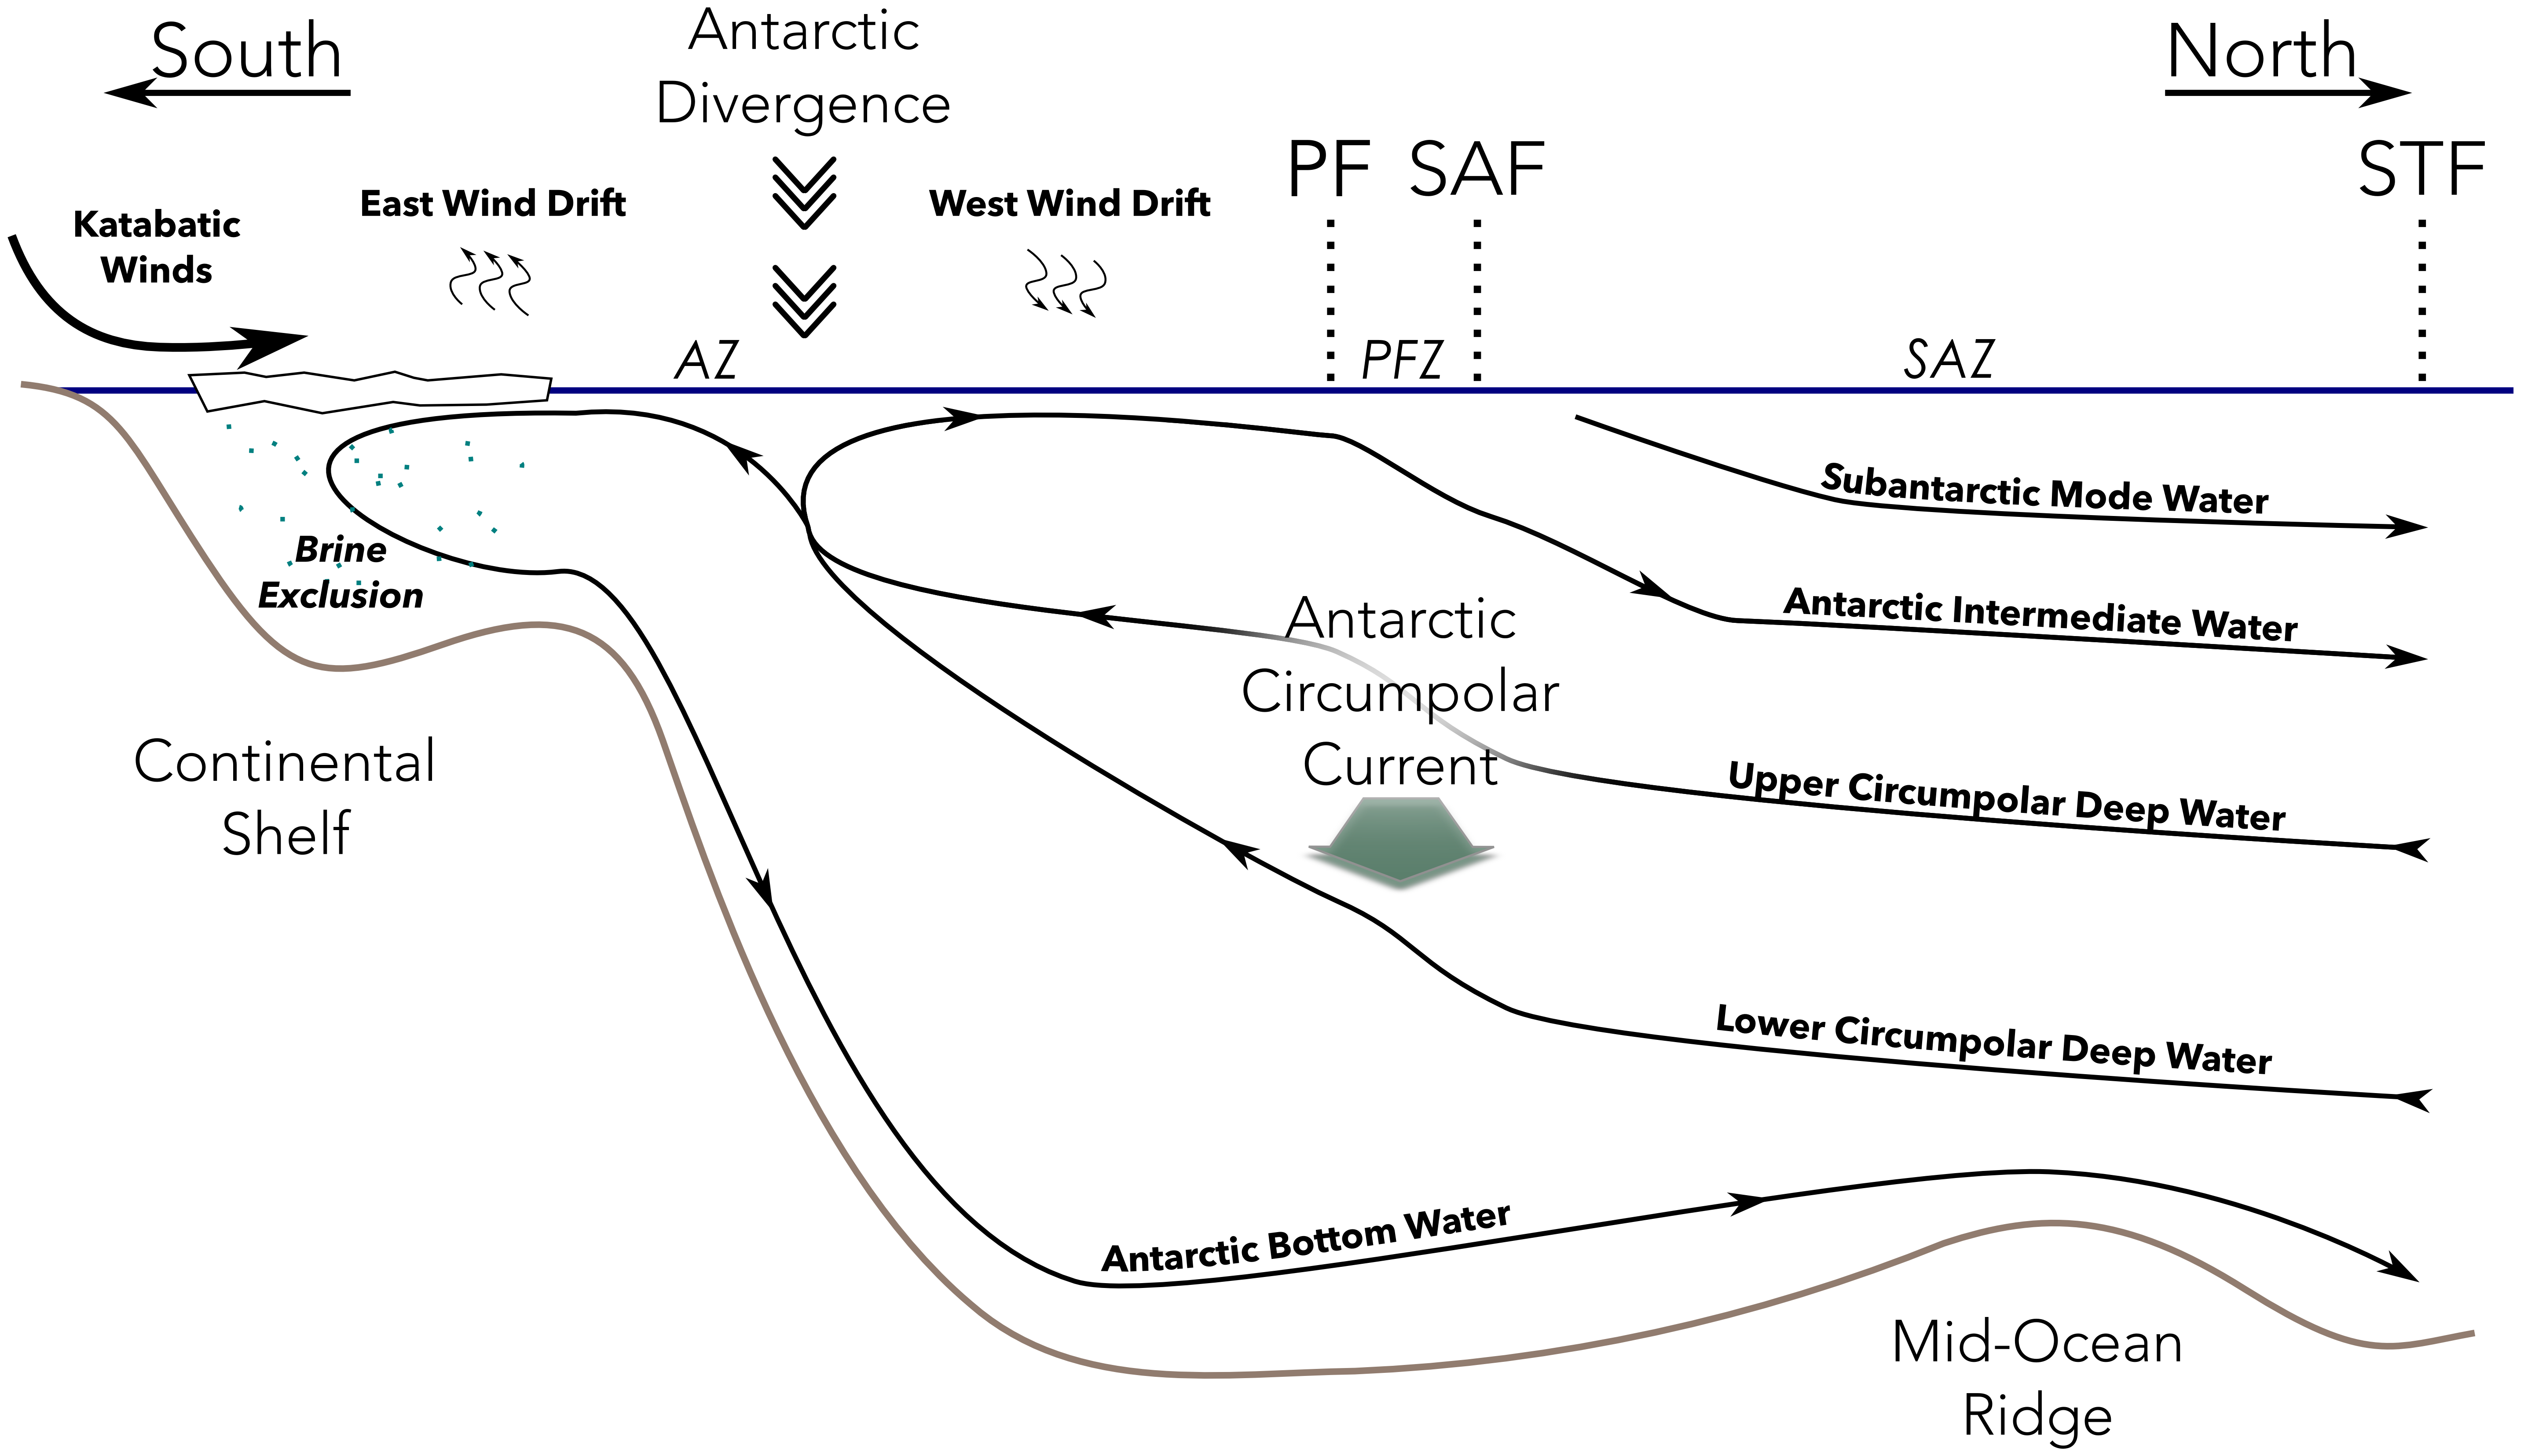
\includegraphics[width=\textwidth]{../introduction/oceanographymap.png}
  \caption[Major fronts and water masses of the Southern Ocean]{North--South cross-section of the Southern Ocean, showing major fronts and water masses.
  This map is schematic only and not to scale.
  Acronyms are as follows: Subtropical Front (STF); Subantarctic Zone (SAF); Subantarctic Front (SAF); Polar Frontal Zone (PFZ); Polar Front (PF); Antarctic Zone (AZ).}
  \label{fig:oceanographymap}
\end{figure}


Definitions of the \ac{SO}'s extent vary.
Features commonly used to define its northern boundary include the 60\textsuperscript{th} parallel south and the \ac{AC}, while most Australian cartographic and governmental bodies consider the \ac{SO} to begin at Australia's southern coastline, or approximately the 45\textsuperscript{th} parallel south.
As these distinctions have no biological relevance, for simplicity the Australian definition will be used in this thesis.

The surface of the \ac{SO} is composed of several distinct zones, separated by circumpolar fronts \figref{fig:oceanographymap}.
Step transitions in the temperature and density of surface waters define the locations and extent of these fronts \cite{Sokolov:2002tc,Orsi:1995va}.
The northernmost front is the \ac{STF}, which lies at \textapprox{}40--45\textdegree{} S, separating the \ac{SAZ} from the warmer and saltier tropical oceans to its north \cite{Sokolov:2002tc}.
Across the \ac{STF}, potential temperature at 150 m depth decreases from \textgreater{} 12 to \textless{} 10 \textdegree{}C.

Moving southwards, the southern extent of the \ac{SAZ} is defined by the \ac{SAF}.
The \ac{SAF} is the northernmost and primary current core of the multiply-branched \ac{ACC} \cite{Sokolov:2009wp}, and its position is thus defined by that of the \ac{ACC} which varies considerably with longitude \cite{Moore:1999to}.
As with the \ac{STF}, there is a drop in potential temperature of 2--4 \textdegree{}C across the front \cite{Sokolov:2002tc}.
The \ac{SAF} also marks the northern boundary of the \ac{PFZ}, where the \ac{SAZ} and colder \ac{AZ} waters meet and mix.
Although both the \ac{SAF} and \ac{PF} represent large step changes in surface characteristics, the \ac{PFZ} itself is relatively constant \cite{WhitworthIII:1987ky}.
This zone, and particularly its bounding fronts, are regions of high primary productivity \citep[e.g.][]{Laubscher:1993hu,Abell:2005ji}.

The southern boundary of the \ac{PFZ} is the \ac{PF}, also a current core of the \ac{ACC}, and associated with a potential temperature drop of \textapprox{}1--1.5 \textdegree{}C \cite{Moore:1999to}.
The waters south of the \ac{PF} constitute the \ac{AZ}, the southernmost and coldest (\textless{} 2 \textdegree{}C, \citet{Sokolov:2002tc}) major zone.
The \ac{AZ} can be further subdivided by several minor features, including the \ac{SACCF} and \ac{SB}, both weaker southern branches of the \ac{ACC}.
However, these do not represent significant step transitions in physical properties.

\subsection{Water masses and circulation}

In addition to these surface features, the \ac{SO} comprises several distinct water masses \figref{fig:oceanographymap}, the circulation of which forms a major component of global \ac{THC}.
The most extensive of these is \ac{CDW}, which consists of two layers.
The \ac{UCDW}, characterised by a nutrient maximum and oxygen minimum, originates in the western Indian and south-eastern Pacific oceans \cite{Orsi:1995va}.
The \ac{LCDW}, characterised by a salinity maximum, originates as sinking \ac{NADW} \cite{WhitworthIII:1987ky}.
Both layers of \ac{CDW} shoal southwards across the \ac{ACC}.

South of the \ac{PF} is the Antarctic Divergence, a region of transition between dominant easterly and westerly winds.
As a consequence of Ekman (i.e. wind-forced) flow, surface currents are divergent, with those to the north driven further northwards by the westerlies (the West Wind Drift) while those to the south are forced southwards by the easterlies (the East Wind Drift) \cite{Foldvik:1988gp}.
This generates a region of upwelling, where the \ac{UCDW} meet and interact with the upper ocean layers and atmosphere.

Between the divergence and the \ac{PF}, the surface layer (\textapprox{}100--300 m depth) consists of \ac{ASW}, which is colder, less saline and better ventilated (i.e.\ more oxygenated) than the \ac{CDW}.
Driven by Ekman transport in the West Wind Drift, the \ac{ASW} moves northwards towards the \ac{PF}, with isopycnals (surfaces of constant potential density) sloping gently downwards towards the north.
At the \ac{PF}, the \ac{ASW} sinks rapidly to form the \ac{AAIW} (\textapprox{}500--1500 m depth), a layer of low-salinity water which underlies \ac{SAZ} and, moving northwards, contributes to the intermediate water of the subtropical oceans \cite{Foldvik:1988gp}.
(Note that both the \ac{SAF} and \ac{PF} can be defined as the locations where the temperature minimum associated with \ac{AAIW} rapidly decreases in depth \cite{WhitworthIII:1987ky}.)
Overlying the \ac{AAIW} in the \ac{SAZ} is the \ac{SAMW}, which forms the surface layer north of the \ac{SAF} \cite{Speer:2000th}.
Although the \ac{SAF} is nominally the southern boundary of the \ac{SAMW}, the surface discontinuity may sometimes occur several degrees to the south of the sub-surface front \citep[e.g.][]{Deacon:1982ce,Orsi:1995va}

Surface and \ac{CDW} waters south of the Antarctic Divergence do not move northwards to form \ac{AAIW}, but instead are driven southwards by the East Wind Drift.
The region between the Antarctic Divergence and the coast is the site of dense, cold \ac{AABW} formation.
Katabatic winds from the Antarctic continent form polynyas and cool the surface waters, while brine exclusion during sea ice formation increases the waters' density.
This newly formed cold and dense \ac{AABW} sinks rapidly and flows down the continental shelf and margin to form an abyssal layer beneath the entire \ac{SO} \cite{Orsi:1999hz,Foldvik:1988gp}.
\ac{AABW} formation does not occur along the entire continental margin; rather, it is concentrated in the Weddell and Ross seas, and to a lesser extent the D'Urville sea off the Ad\'{e}lie Land coast.
\ac{AABW} is a major source of abyssal water to the World Ocean, and its formation drives global \ac{THC}.
Because \ac{AABW} is ventilated in the \ac{SO} before sinking rapidly, \ac{AABW} is relatively enriched in oxygen compared to other deep layers of the World Ocean, which are oxygen-depleted due to the heterotrophic oxidation of sinking organic matter.

\subsection{Effect of climate change}

Anthropogenic climate change is having a significant effect on the \ac{ACC} and the water masses it defines.
Changes in the \ac{SAM}, a regular pattern of Southern Hemisphere atmospheric circulation characteristics, are leading to an intensification of the westerly winds \cite{Thompson:2002ic} which drive the \ac{ACC}.
As a consequence of this and other climate change-related effects, the mean annual path of the \ac{ACC} and its associated fronts and isopycnals has moved \textapprox{}50 km southwards since the 1950s \cite{Gille:2002fr}.
Waters on the poleward side of the \ac{ACC} have become warmer and more saline, while those to the north cooler and fresher \cite{Boning:2008il}.
The \ac{ACC} itself is warming and freshening \cite{Boning:2008il}, from the surface to 900 m depth \cite{Aoki:2003fo}.

\citet{Fyfe:2005vp}, using a wind-driven model of the southward shift of the \ac{ACC}, predicted that with conservative assumptions about future anthropogenic greenhouse gas emissions (\ac{IPCC} A2 and B2 scenarios), the \ac{ACC} can be expected to move \textapprox{}1.4\textdegree{} southwards by the year 2100.
They note that this is equivalent to reducing the volume of the \ac{SO} south of the \ac{ACC} by about $16 \times{} 10^{6}$ \ce{km^{3}}, or approximately the volume of the Arctic Ocean.

Aside from the oceanographic effects, these changes can be expected to effect the biology of the \ac{SO}.
In particular, even neglecting the changes in temperature and salinity of the water masses defined by the \ac{ACC}, the southward migration of the \ac{ACC} and concomitant change in the relative volumes (and surface areas) of the water masses it defines are a significant change in the size of the microbial habitats these masses represent.
Predicting the effects this will have on \ac{SO} ecosystems and ecosystem functions requires an understanding of the microbial ecology of the \ac{SO}, and its biogeography relative to the \ac{ACC} and its associate fronts and water masses.
The following section gives an overview of the current state of knowledge.

\section{Microbial ecology of the Southern Ocean}

As in all the World Ocean, microorganisms perform key ecosystem functions in the \ac{SO}, driving carbon, nitrogen, sulfur and other major cycles.
There is evidence that the \ac{PF} and other \ac{SO} fronts are biogeographic boundaries between distinct bacterioplankton communities \citep[e.g.][]{Selje:2004ka,Abell:2005ji,Giebel:2009hr,Weber:2010fi}.
This section reviews the current state of knowledge on the abundance, biogeography and ecosystem functions of microorganisms in the \ac{SO}, with a focus on molecular studies.

Eukaryotic phytoplankton and protists are a major component of the \ac{SO} microbial ecosystem.
In particular, they perform a large proportion of primary production in coastal and continental shelf \ac{AZ} waters \citep[e.g.][]{ElSayed:2005jq}.
Additionally, the production and deposition of biogenic silica by \ac{SO} diatoms composes a large fraction of the global silica flux \cite{Treguer:1995kz}.
However, as the work described in this thesis focuses on bacteria and archaea, eukaryotic plankton will not be considered except where relevant to bacteria, archaea or viruses (e.g.\ grazing).

\subsection{Bacteria}

\subsubsection{Alphaproteobacteria}

\subsubsubsection{Roseobacter clade}

The Roseobacter clade is an abundant and ecologically significant group of marine bacteria, found at high (> 15\%) abundance in most marine surface environments \citep[][and references therein]{Buchan:2005hd}.
Unlike some other major proteobacterial groups that are strongly associated with a particular ecological niche (e.g.\ the SAR11 clade), roseobacters have diverse metabolic abilities, with members capable of (for example) aerobic anoxygenic phototrophy \cite{Biebl:2005fp,Beja:2002gt}, degradation of \ac{DMSP} by at least two pathways \cite{Miller:2004jz,Moran:2003cwa}, carbon monoxide oxidation \cite{King:2003kc} and heterotrophic utilisation of a broad range of substrates \citep[reviewed in][]{Brinkhoff:2008do}.
Roseobacters are found in the planktonic fraction as well as in commensal association with phytoplankton and metazoans \citep[reviewed in][]{Buchan:2005hd}.

Several 16S rDNA-based studies have identified the \ac{RCA} subgroup as ubiquitous and abundant in \ac{SO} surface waters and to a depth of at least 2200 m, composing \textapprox{}10--30\% of surface bacteria (and the majority of roseobacters) in the Subantarctic and Antarctic zones \cite{Giebel:2009hr,Murray:2007db,Ghiglione:2011ee} and a major fraction of the population in coastal waters \cite{Murray:2007db,Koh:2011ij}.
Two major \ac{RCA} phylotypes appear to be present in the \ac{SO} and form the majority of the Roseobacter population.
The phylotypes are strictly segregated by the \ac{PF}, coexisting only within the \ac{PFZ} \cite{Selje:2004ka,Giebel:2009hr} where they may outnumber even the SAR11 clade.
There is some evidence that the \ac{AZ} \ac{RCA} phylotype originates from the North Atlantic; \citet{Giebel:2009hr} noted \ac{CDW} at 2200 m in the \ac{SZ} had an identical temperature-salinity signature to \ac{NADW}.
\ac{NADW} is formed by the sinking of dense, saline waters from the surface north Atlantic, and is transported to the \ac{SO} via global thermohaline circulation to become \ac{CDW} \cite{Callahan:1972tk}.
Consistent with the upwelling of \ac{CDW} in the \ac{AZ} south of the \ac{PF}, \citep{Selje:2004ka} reported in a global study of \ac{RCA} 16S rDNA gene fragments that the surface phylotype south of the \ac{PF} was identical to one found in the Arctic Ocean, while differing by 3 bp from that north of the \ac{PF}.

Little is known about the functional capabilities of \ac{RCA} as only two isolated representatives have been described to date.
\citep{Giebel:2010bsa} isolated \candidatus{Planktomarina temperata} from the North Sea, where it was the dominant phylotype.
The authors' identification of the pufM gene encoding a bacteriochlorophyll a subunit suggests at least this member of the \ac{RCA} is capable of performing aerobic anoxygenic photosynthesis, a function of potentially large ecological significance.
\citet{Mayali:2008eb} isolated an apparently heterotrophic \ac{RCA} member from subtropical waters, and found \emph{in vitro} evidence that they colonised and increased mortality in blooming dinoflagellates, but did not investigate photosynthetic potential.

Roseobacters, and particularly the \ac{RCA}, have been strongly associated with phytoplankton blooms in the \ac{SO}.
Two separate 16S rDNA-based studies of a naturally fertilised bloom in the Kerguelen islands region \cite{West:2008kc,Obernosterer:2011df} found that \ac{RCA} and the Roseobacter NAC11-7 and NAC11-6 clusters were dominant bacterial \acp{OTU} in the bloom patch, suggesting they play a role in heterotrophic degradation of bloom products.
Unlike the other clusters, however, \ac{RCA} representatives were also relatively abundant and metabolically active outside of the patch.
Both \citet{Giebel:2009hr} and \citet{Obernosterer:2011df} found that in \ac{SO} vertical profiles \ac{RCA} abundances often peaked at the \ac{DCM}, again suggesting an association with phytoplankton.

\ac{RCA} abundance may follow a seasonal cycle in the \ac{SO}.
\citet{Giebel:2009hr} found that \ac{RCA} phylotypes composed at most 8\% of all bacterial 16S rDNA genes during winter but up to 36\% in the coastal current and Weddell sea during autumn, while \citet{Ghiglione:2011ee} found the proportion to peak in January in coastal waters off the Antarctic Peninsula and in February off the Kerguelen islands. 

A metagenomic study of \ac{SO} waters off West Antarctica found that Roseobacter clade \ac{SSU} rRNA sequences were much more abundant in summer than in winter, with \genus{Sulfitobacter} sequences the most abundant within this clade \cite{Grzymski:2012ej}.
This is consistent with the association of roseobacters with phytoplankton \cite{Moran:2003cwa}.
Nevertheless, Roseobacter clade representatives in these polar waters are metabolically active in both seasons, expressing high-affinity uptake systems (ABC, TRAP) for capturing labile nutrients such as sugars, polyamines, amino acids, and oligopeptides \cite{Williams:2012bs}.

\subsubsubsection{SAR11}

The SAR11 clade of Alphaproteobacteria is probably the most abundant class of marine microorganisms worldwide \cite{Morris:2002bn}.
\candidatus{Pelagibacter ubique} strain HTCC1062, the first and most intensively studied SAR11 isolate, has one of the smallest genomes and gene complements of any known free-living cell as well as a very small cell volume \cite{Giovannoni:2005ib}.
The small volume, streamlined genome and high proportion of ABC nutrient-uptake transporter genes are all consistent with an oligotrophic lifestyle, scavenging a wide range of substrates using high-affinity, broad-specificity transporters \cite{Giovannoni:2005ib,Lauro:2009gx,Sowell:2008ks}.
SAR11 cells probably preferentially consume low over high molecular weight \ac{DOM} \cite{Malmstrom:2005el} and their relative contribution to uptake of \ac{DOM} may decrease as substrate concentration increases \cite{Alonso:2006dj}.
A consequence of this oligotrophic strategy is that SAR11 members are probably unable to take advantage of sudden nutrient influxes, such as during phytoplankton blooms, to rapidly increase cell density \cite{Tripp:2008dd}.

SAR11 has been consistently detected at high abundances in molecular surveys of the \ac{SO}, in all open ocean regions as well as at depth and in coastal waters, and is usually the dominant alpha-proteobacterial, if not bacterial, group \cite{Giebel:2009hr,Murray:2007db,LopezGarcia:2001vp,Straza:2010io,Jamieson:2012up,GarciaMartinez:2000fu,Ghiglione:2011ee,Murray:2011ib,Piquet:2011fj}.
It is probably more abundant in the epipelagic than at depth \cite{Giebel:2009hr}.

SAR11 seems to exhibit biogeographic partitioning in the \ac{SO}, and is probably represented by two major ecotypes with a temperature-driven boundary in the region of the \ac{PF} \cite{Brown:2012gna}.
It is probably more abundant in the \ac{SAZ} and \ac{PFZ} zones than in the \ac{AZ} \cite{Giebel:2009hr,Ghiglione:2011ee}.
This may be related to a competitive advantage of the oligotrophic SAR11 in the \ac{HNLC} \ac{SAZ} relative to the \ac{AZ}, where blooming phytoplankton lead to increased concentrations of \ac{HMW} \ac{DOM} and \ac{POM}.
\citet{Straza:2010io} found SAR11 accounted for the largest fraction of leucine uptake among all bacterial groups in continental shelf waters off the West Antarctic Peninsula, but a comparatively small fraction of protein uptake, consistent with a role as a \ac{LWM} \ac{DOM} specialist.
\citet{West:2008kc}, examining 16S rDNA profiles in and out of a natural phytoplankton bloom on the Kerguelen Plateau (\ac{SAZ}), found SAR11 to be a dominant group in \ac{HNLC} waters outside the bloom patch but relatively less abundant in it.
A separate study of the same bloom found SAR11 had a markedly smaller relative contribution to bulk leucine incorporation in the patch than out, suggesting it was not a major contributor to \ac{DOM} degradation \cite{Obernosterer:2011df}.
Interestingly, SAR11 did dominate in abundance and leucine incorporation at an additional site where a recent and transient phytoplankton bloom had taken place, implying a time lag in the succession between the baseline \ac{HNLC} and bloom populations.
The authors additionally noted that SAR11 abundances at the bloom station began to climb towards non-bloom levels once the bloom had peaked and begun declining.
An Antarctic Peninsula SAR11 metaproteome was dominated by ABC transport proteins for the capture and uptake of labile substrates, especially taurine, polyamines and amino acids, and also included \ac{DMSP} demethylase \cite{Williams:2012bs}.
Finally, despite an apparently negative correlation between SAR11 and blooming phytoplankton, \citet{Ghiglione:2011ee} found only small seasonal changes in abundance during an annual cycle at the \ac{AP} and Kerguelen Island.
These studies are all consistent with the view of SAR11 as a typically non-opportunistic oligotroph specialising in \ac{LWM} \ac{DOC}.

One of the most interesting physiological features of SAR11 representatives is their expression of the retinal-binding pigment proteorhodopsin, which has been shown to act as a proton pump when exposed to light \cite{Anonymous:2012ck} and has therefore been implicated in photoheterotrophy.
Surprisingly, given very low light levels in Antarctic waters during austral winter, SAR11 proteorhodopsin is present throughout the annual cycle \cite{Williams:2012bs}.
This may be consistent with the observation that many marine proteorhodopsins do not appear tuned to maximise energy conversion from available light, which has led \citet{Fuhrman:2008he} to propose at least some proteorhodopsins may perform non-energetic functions such as photoregulatory sensing.
Alternatively, constitutive expression of proteorhodopsin for light harvesting in SAR11 may facilitate the ability to immediately respond to cellular energy deficits caused by carbon starvation \cite{Steindler:2011hk}.

\subsubsubsection{SAR116}

The SAR116 clade of Alphaproteobacteria has been detected throughout the world ocean, including in molecular studies of the \ac{SO} \cite{West:2008kc,Topping:2006ul}.
 \citet{Topping:2006ul} using \ac{FISH} estimated it composed 13.1\% $\pm 8.6$ to 31.9\% $\pm13.7$ of bacterioplankton in the West and East regions of the Scotia Sea respectively.

The only isolated and fully sequenced SAR116 representative, \candidatus{Puniceispirillum marinum}, has been reported to have a versatile repertoire of genes for aerobic CO fixation, C1 metabolism and dimethylsulfoniopropionate degradation, suggesting it may occupy a ``marine generalist'' niche similar to that of SAR11 and some roseobacters \cite{Oh:2010di}.
Proteins for ABC and TRAP transport and C1 metabolism with high matches to SAR116 bacteria were detected in both the summer and winter metaproteomes of coastal waters of the Antarctic Peninsula, consistent with a preference for labile compounds and C1 substrates \cite{Williams:2012bs}.

\subsubsection{Betaproteobacteria}

The Betaproteobacteria are a large and cosmopolitan class with a range of ecological roles in the World Ocean \citep[reviewed in][]{Kirchman:2008wz}.
\citet{Hollibaugh:2002em} detected \genus{Nitrosospira}-like 16S rRNA sequences in Ross Sea and Antarctic Peninsula surface waters, and noted that the ribotype appeared similar to one found in the Arctic.
While not found at high abundance \cite{Gentile:2006ef,Ghiglione:2011ee,Jamieson:2012up}, there is evidence that Betaproteobacteria perform significant ecological functions.
Most known \ac{AOB} belong to the Betaproteobacteria \cite{Head:1993vt,Teske:1994wt}.
Metagenomic and metaproteomic analyses of surface coastal waters off the Antarctic Peninsula show evidence of Calvin cycle carbon fixation and ammonia oxidation in winter by Betaproteobacteria \cite{Grzymski:2012ej,Williams:2012bs}.

The OM43 clade of Betaproteobacteria has been associated with coastal phytoplankton blooms \cite{Morris:2006hma} and shown to be an obligate methylotroph capable of using methanol and formaldehyde as carbon and energy sources \cite{Giovannoni:2008kw}.
As it has the smallest reported genome for a free-living cell, OM43 seems to be highly specialized for this unusual niche (the ``genome streamlining'' hypothesis, \citet{Mira:2001ti}).
OM43 has been detected in a 16S rDNA library in a naturally fertilised bloom in the \ac{SAZ} \cite{West:2008kc}, where it was the only betaproteobacterial representative, and in a metaproteomic survey of coastal waters on the \ac{AP}, where methanol dehydrogenase from OM43 was detected \cite{Williams:2012bs}.
Although the source of methanol in the marine environment is not yet clear, it may be a byproduct of phytoplankton growth \cite{Heikes:2002ee}, which would be consistent with OM43's observed association with coastal blooms.
This possibility suggests OM43, and perhaps other C1 specialists, play an underexplored role in the marine microbial loop.
Alternative methanol sources are atmospheric deposition \cite{Sinha:2007uu} or photochemical degradation of organic material \cite{Dixon:2011er}.
The latter is of particular interest in Antarctic waters, given the high levels of solar irradiation during the austral summer.

\subsubsection{Gammaproteobacteria}

\subsubsubsection{SAR86}

The gammaproteobacterial SAR86 clade is an abundant group in the surface ocean, being e.g.\ the most abundant genome of an uncultured organism in the \ac{GOS} dataset \cite{Dupont:2011fk}.
While it has been detected in the Southern Ocean \cite{Abell:2005ji,Topping:2006ul,West:2008kc,Obernosterer:2011df}, little is known of its distribution or ecological role.
\cite{Topping:2006ul} estimated on the basis of \ac{FISH} activity that SAR86 cells composed 7.8\% $\pm8.2$ and 18.3\% $\pm17.0$ of total bacterioplankton in the western and eastern Scotia Sea respectively, suggesting that at least in the SAZ it is a major component of the surface community.
Genomic analysis of partial SAR86 genomes assembled from metagenomes found the clade have streamlined genomes and are specialized for utilizing lipids and carbohydrates, suggesting minimal competition between SAR86 and SAR11 for \ac{DOC} \cite{Dupont:2011fk}.
This may be reflected by the simultaneous high abundance and activity of SAR11 and SAR86 in the \ac{HNLC} waters of the \ac{SAZ} \cite{Obernosterer:2011df}

\subsubsubsection{OMG group}

The term \ac{OMG} was named for a group of physiologically diverse heterotrophs that belong to previously detected environmental rRNA clades (OM60, BD1-7, KI89A, OM182, SAR92) \cite{Cho:2004gm}.
Cultured \ac{OMG} isolates have been shown to be obligately oligotrophic \cite{Cho:2004gm}.
Nevertheless, SAR92 is associated with nutrient-rich waters with high phytoplankton abundances \cite{Stingl:2007ja,Pinhassi:2004is}.
Reports of SAR92 in the \ac{SO} corroborate this ecology: both \citet{West:2008kc} and \citet{Obernosterer:2011df} found SAR92-affiliated \acp{OTU} to be far more abundant inside the \ac{KEOPS} phytoplankton bloom patch than in typically \ac{HNLC} \ac{SAZ} waters outside of it, with abundance declining as the bloom aged.
This, combined with the observation that SAR92 growth is highly carbon-limited \cite{Stingl:2007ja}, suggests the clade plays an important role in degradation of organic carbon produced by phytoplankton blooms.
It has also been detected in coastal \ac{AP} and Kerguelen Islands waters \cite{Ghiglione:2011ee}.
Metaproteomic and metagenomic surveys of coastal waters at Palmer station found \ac{OMG} to be more abundant in the summer than winter \cite{Williams:2012bs}.
TonB-dependent receptor systems from \ac{OMG} were highly abundant in the metaproteome, indicating that this is the preferred uptake system of ambient substrates \cite{Williams:2012bs}.
Certain \ac{OMG} strains encode proteorhodopsin (HTCC2207, \citet{Stingl:2007ja}; HTCC2143, \citet{Oh:2010di}), also indicated in the metaproteomic study in both seasons \cite{Williams:2012bs}.

\subsubsubsection{Ant4D3}

In a study of six fosmids from nearshore waters at Palmer station, \citet{Grzymski:2006ds} identified a uncultured gammaproteobacterium, Ant4D3.
It has since been reported as one of the dominant proteobacterial groups in the \ac{SO}.
In waters off the western Antarctic Peninsula, Ant4D3 was reported to compose 10\% of the total community and half the gammaproteobacterial community, and 68\% of cells incorporating amino acids \cite{Straza:2010io}.
The authors also reported that the clade appears to have low diversity, based on detected rDNA sequences.
Like SAR86, Ant4D3 cells were more active in \ac{HNLC} than bloom conditions on the Kerguelen Plateau \cite{West:2008kc}.
However, \citet{Ghiglione:2011ee} reported that 16.5\% of tag-pyrosequenced 16S \ac{DGGE} bands from summer \ac{AP} waters were affiliated to Ant4D3, dominating the Gammaproteobacteria and outnumbering winter and Kerguelen Island waters.
\citet{Murray:2011ib} similarly found Ant4D3 clones to be highly abundant in a 16S library from waters in the vicinity of Antarctic icebergs.
Little is known about the group's function or ecological position, although it has been detected in Arctic waters where it appeared to occupy a \ac{DOM} utilisation niche different from that of other major heterotrophs e.g.\ SAR11 \cite{Nikrad:2012fa}.

\subsubsubsection{GSO-EOSA-1}

The GSO-EOSA-1 cluster of sulfur-oxidizing Gammaproteobacteria, which includes the uncultivated ARCTIC96BD-19 and SUP05 lineages as well as cultivated chemoautotrophic clam symbionts, has been reported in global mesopelagic waters \cite{Swan:2011hb} and oxygen minimum zones \cite{Walsh:2009fja,Canfield:2010ib}.
Three studies have recently identified GSO-EOSA-1 representatives at high abundance in coastal and \ac{AZ} waters.
A metagenomic survey of coastal waters at Palmer station found GSO-EOSA-1 winter bacterioplankton were dominated by Gammaproteobacteria (19.7\% of the winter library compared to 2.7\% of the summer library) falling into five closely-related (0.03 distance) bins that were affiliated with the GSO-EOSA-1 complex.
\citet{Grzymski:2012ej}, in a metaproteomic survey of coastal waters at Palmer station, found GSO-EOSA-1 proteins composed a large fraction of all gammaproteobacterial proteins detected and were significantly more abundant in winter than summer (20\% vs 3\%).
In a companion metaproteomic analysis of the same sites, \citet{Williams:2012bs} confirmed this high abundance and seasonal pattern, although GSO-EOSA-1 appeared to be metabolically active at the surface in both summer and winter.

Genomic and metaproteomic analyses of GSO-EOSA-1 representatives, particularly SUP05, have revealed the potential for carbon fixation via the Calvin cycle and sulfur oxidation, even in well-oxygenated waters \cite{Walsh:2009fja,Swan:2011hb,Grzymski:2012ej}.
\citet{Grzymski:2012ej} estimated from rRNA abundances that 18--37\% of the winter bacterioplankton community comprises \acp{OTU} with the potential for chemolithoautotrophy, including GSO-EOSA-1, suggesting winter chemolithoautotrophy may contribute significantly to \ac{SO} carbon fixation.

\subsubsection{Deltaproteobacteria}

Deltaproteobacteria are rarely detected at abundance in global surface waters \citep[see e.g.][]{Venter:2004hg}, and this pattern appears to hold in the Southern Ocean \cite{Murray:2007db,West:2008kc,Ghiglione:2011ee,Murray:2011ib,Ducklow:2011jl,Jamieson:2012up}.
However, they may increase in abundance in mesopelagic waters \cite{Wright:1997vg,Pham:2008bba}.
At a 3000 m deep site at the \ac{PF} in the Drake Passage, \citet{LopezGarcia:2001vp} detected several deltaproteobacterial 16S rDNA sequences, all of which clustered with the marine deltaproteobacterial clade SAR324 previously identified in the mesopelagic Sargasso Sea \cite{Wright:1997vg}.
Whole-genome analysis of SAR324 indicates an ecology that includes carbon fixation via the Calvin cycle and sulfur oxidation, as well as oxidation of methylated compounds \cite{Swan:2011hb}.
SAR324 may therefore be significant contributors to chemoautotrophy in the dark ocean \cite{Swan:2011hb}.

\subsubsection{CFB}

Bacteria of the group \ac{CFB} are cosmopolitan and abundant in the world ocean \cite{Glockner:1999vm}.
While the \ac{CFB} often form a major fraction of planktonic taxa \cite{Fandino:2001uw}, they are particularly prevalent in particle-attached communities \cite{DeLong:1993uu} and are associated with blooming phytoplankton \cite{Pinhassi:2004is}.
Isolated \ac{CFB} representatives have a well-described aptitude for the degradation of \ac{HMW} \ac{DOM}, particularly biopolymers which may be recalcitrant to utilisation by other bacterial heterotrophs \citep[reviewed in][]{Kirchman:2002ub}, suggesting they play an important role in remineralisation of primary production products.
Of the \ac{CFB}, the class Flavobacteria seem to be in the majority worldwide in both freshwater and marine environments \cite{OSullivan:2006km,Cottrell:2005bo} including the Southern Ocean \cite{Abell:2005ji}.

\ac{CFB} in the \ac{SO} are strongly biogeographically partitioned.
\citet{Abell:2005ji}, using \ac{DGGE} and 16S sequencing with Flavobacteria-specific primers, found significantly higher abundance and diversity of particle-attached Flavobacteria in the nutrient- and phytoplankton-rich waters south of the \ac{PF} relative to the \ac{HNLC} waters of the Subantarctic.
This difference in abundance may be largely attributable to the low iron availability in the Subantarctic, which probably limits primary production \cite{Boyd:2007ij}.
Both natural and artificial iron fertilization events in the Subantarctic have resulted in high abundances of bacterial heterotrophs \cite{Christaki:2008el,Oliver:2004ty}; \citet{West:2008kc} identified the \ac{CFB} as a major component of the bacterial response to blooms induced by natural iron input on the Kerguelen plateau.
The higher abundance of \ac{CFB} in the \ac{AZ} may also relate to their prevalence in sea ice \cite{Brinkmeyer:2003iq,Brown:2001hh}, from which they would be released into \ac{AZ} waters during seasonal melting.
Two groups, the uncultured agg58 cluster and the genus \genus{Polaribacter}, appear to dominate \ac{CFB} populations and activity in the \ac{SO} \cite{Murray:2007db,Abell:2005dh,Abell:2005ji,Obernosterer:2011df,West:2008kc,Ghiglione:2011ee,Ducklow:2011jl,Straza:2010io}.

There is some evidence that planktonic and particle-attached \ac{CFB}, rather than being an integrated population with cells opportunistically shifting between phases, may comprise at least partially distinct groups of phylotypes.
In a mesocosm experiment examining colonisation of diatom detritus in \ac{SO} seawater, 16S \ac{DGGE} and sequencing analysis showed a large proportion of flavobacterial phylotypes present in the planktonic phase failed to colonise detrital particles during the course of the experiment \cite{Abell:2005dh}.
The authors suggest these phylotypes may be slower-growing, perhaps comprising a secondary group of colonisers which only come to dominate when the more accessible detrital nutrients have been exhausted and the primary colonisers have secreted useful secondary metabolites.
Alternatively, some flavobacterial groups may not use particle attachment as a primary strategy.

\citet{Kirchman:2002ub} suggests 16S clone libraries may systematically underestimate the abundance of \ac{CFB} in environmental samples, noting that in two studies where both \ac{FISH} and 16S analysis were employed at the same site there were common discrepancies in \ac{CFB} abundance estimates between the two methods \cite{Cottrell:2000iq,Eilers:2000in}.
Additionally, both \ac{FISH} and PCR based methods may underestimate \ac{CFB} abundance relative to metagenomic surveys, due to probe specificity biased against Bacteroidetes 16S rDNA \cite{Cottrell:2005bo,OSullivan:2006km}.

\genus{Polaribacter} is a gas-vacuolated, proteorhodopsin-expressing flavobacterial genus prevalent in Arctic and Antarctic seawater.
Its genome indicates a preference for polymers obtained from algal detritus rather than labile exudates (e.g.\ taurine, polyamines) \cite{Gonzalez:2008tn}.
An Antarctic Peninsula coastal metagenome found \genus{Polaribacter}-related sequences to be dominant in summer, consistent with an association with phytoplankton blooms and/or input from melting sea-ice \cite{Grzymski:2012ej}.
Flavobacterial proteins (including those with the best matches to \genus{Polaribacter} spp.) were similarly much more abundant in the summer than winter metaproteome from the same sites, with components of TonB-dependent receptor systems predominating \cite{Williams:2012bs}. 

\subsubsection{Cyanobacteria}

Cyanobacteria, dominated by the genera \genus{Prochlorococcus} and \genus{Synechococcus}, are the most abundant photosynthetic organisms on Earth \citep[][and references therein]{Scanlan:2009cw}, but little molecular research has been performed on their role in \ac{SO} ecosystems.
This may be because it has been generally accepted that there are no cyanobacteria in \ac{AZ} waters \cite{Ghiglione:2011ee,Zubkov:1998uf,Evans:2011ih}, although recent and metaproteomic results \cite{Williams:2012bs} challenge this assumption.
It is not infeasible that cyanobacteria survive at Antarctic temperatures, as (apparently psychrophilic or psychrotolerant) \genus{Synechococcus} and \genus{Prochlorococcus} strains have been identified in several marine-derived Antarctic lakes, including at sub-zero water temperatures \cite{Bowman:2000ef,Powell:2005uh,Lauro:2010jna}.
Regardless, it is clear that cyanobacteria, if present in the \ac{AZ}, are at very low abundance \cite{Marchant:1987wv} and probably of little ecological significance.
Cyanobacteria also appear to be at low abundance in the \ac{SAZ} \cite{Abell:2005ji,Topping:2006ul}.  

\subsubsection{Verrucomicrobia}

Verrucomicrobia is a recently described phylum, members of which are ubiquitous in the marine environment, and which appears to be composed of several physiologically distinct lineages \cite{Freitas:2012jz}.
A small number of Verrucomicrobia representatives have been detected in the \ac{SO} \cite{Murray:2011ib,West:2008kc,Gentile:2006ef,Murray:2007db}, and \citet{Ghiglione:2011ee} reported a higher abundance of 16S rDNA clones affiliating with the Verrucomicrobia at a Kerguelen Island site relative to a site near Palmer Station on the Antarctic Peninsula.
Little else is known regarding their abundance, diversity or ecological role in the \ac{SO}.

\subsubsection{Other bacteria}

Other bacterial groups have been reported at low abundance in \ac{SO} waters, including Actinobacteria \cite{Bowman:2003fa,Brinkmeyer:2003iq,Abell:2005ji,Gentile:2006ef,Murray:2007db,Murray:2011ib,Ghiglione:2011ee,Piquet:2011fj,Jamieson:2012up}, Epsilonproteobacteria \cite{Gentile:2006ef,Murray:2007db}, and Firmicutes \cite{Murray:2007db,Anonymous:2011bw,Murray:2011ib}.
Little is known about their respective ecological roles, although Actinobacteria have been associated with marine aggregates \cite{Grossart:2006ez}; interestingly, their terrestrial counterparts have diverse \ac{HMW} substrate degradation capabilities \citep[reviewed in][]{Kirchman:2008wz}.
A strong negative correlation has been reported between actinobacterial abundance and latitude in a global survey of 16S rDNA clone libraries \cite{Pommier:2007vz}, with higher abundances in tropical and subtropical waters, as for Cyanobacteria.

Bacteria of the phylum Planctomycetes have been detected at low abundance in \ac{SO} molecular surveys \cite{Gentile:2006ef,LopezGarcia:2001vp,Jamieson:2012up,Murray:2011ib,Abell:2005ji}.
The Planctomycetes are emerging as organisms of interest in marine microbial ecology, for example as performers of \ac{anammox} \cite{Strous:1999wj}.
They have been identified in a metaproteome from West Antarctic coastal waters \cite{Williams:2012bs}, where they and members of the phylum Nitrospirae were implicated in nitrification using nitrite generated by \ac{AOA} and \ac{AOB}.

\subsection{Archaea}

\citet{DeLong:1994id} first reported the high abundance (up to 34\%) of archaea in Antarctic coastal surface waters, a surprising discovery at a time when the Archaea were generally considered a rare group of strict extremophiles.
The majority of rDNA clones they identified were affiliated with the \ac{MGI}, while the remainder represented the \ac{MGII}.
Subsequent rRNA-based studies are likewise in agreement that \ac{MGI} are the dominant group of archaea in surface waters of coastal Antarctica, followed by \ac{MGII} (Gerlache Strait, \citet{Massana:1998tn}; near Anvers Island, \citet{Murray:1998wy}).
Further rRNA-based analysis showed the widespread distribution of Antarctic marine archaea \cite{Murray:1999tx,Topping:2006ul,Jamieson:2012up}, and identified a significant \ac{MGI} community in benthic sediments on the Antarctic coast \cite{Bowman:2003fa}.

For \ac{MGI}, ammonia-oxidizing chemolithoautotrophy is likely the dominant metabolic lifestyle \cite{Ingalls:2006kv,Berg:2007fj}, suggesting they play major roles in nitrification and carbon fixation in the \ac{SO}.
In a winter coastal Antarctic metaproteome, \ac{MGI} proteins made up 30\% of all identified proteins from bacteria or archaea; no \ac{MGI} proteins were detected in the summer metaproteome \cite{Williams:2012bs}.
The winter metaproteome included \ac{MGI} proteins from the 3-hydroxypropionate/4-hydroxybutyrate cycle, the pathway used by ammonia-oxidizing \ac{MGI} for carbon fixation, and for ammonium transport and oxidation, supporting a nitrification role for Southern Ocean \ac{MGI} \cite{Williams:2012bs}.
The complementary metagenomic analysis of \citet{Grzymski:2012ej} proposed chemolithoautotrophy carried out by ammonia-oxidizing \ac{MGI} and sulfur-oxidizing Gammaproteobacteria (see GSO-EOSA-1, above) to be the major drivers of winter carbon fixation in \ac{AZ} waters.
In summer autotrophic carbon assimilation is driven by algal-driven oxygenic photoautotrophy, consistent with high light availability and intensity, whereas in the polar winter ``dark'' chemoautotrophy by archaea and bacteria plays a major role in carbon fixation.

\citet{Murray:1998wy} found that total archaeal rRNA levels decreased during summer, and noted a negative correlation between archaeal rRNA levels and chlorophyll \emph{a} concentration.
\citet{Massana:1998tn} also observed a decline in archaeal rRNA levels during spring.
\citet{Church:2003vt} found a significantly higher (44\% increase) abundance of \ac{MGI} in surface waters in winter than summer.
Ammonia-oxidizing \ac{MGI} have been shown to be especially sensitive to photoinhibition \cite{Merbt:2011bl}, which might account for their decline during periods of extended illumination.
It has also been speculated that the decline of archaea during spring/summer represents competition with non-archaeal microbes during phytoplankton blooms \cite{Massana:1998tn}, or that the majority of \ac{MGI} were chemoautotrophic and therefore more competitive than heterotrophs during carbon-scarce winter conditions \cite{Murray:1998wy}.
Genomic evidence suggests \ac{MGII} are motile, proteorhodopsin-expressing photoheterotrophs that specialize in protein and lipid degradation \cite{Iverson:2012kc}.
This is consistent with evidence that this group, in contrast to \ac{MGI}, was more relatively abundant at the surface than at depth \cite{Massana:1998tn}.
\citet{Murray:1998wy} noted an increase in \ac{MGII} in autumn in waters off Anvers Island; but otherwise the seasonal distribution of this group in Antarctic waters is not well understood.

The numerical dominance of \ac{MGI} over other archaeal groups in surface and photic zone waters has also become well established \citep[e.g.][]{DeLong:1994id,Massana:2000bg}, although not in aphotic waters; \citet{LopezGarcia:2001vp} detected only euryarchaeaotal sequences in a sample from 3000 m depth at the \ac{PF} in the Drake Passage, including marine groups II and III and a novel marine group IV.
However, these studies also illustrated a potential hazard of probe-dependant methods, namely the high variability of abundance estimates depending on probe design.
For example, \cite{Simon:1999ux} did not detect any DAPI-positive archaeal cells in a summer transect between the polar front and ice edge using the archaea-specific probes ARCH334 and ARCH915, in contrast to the results of several other studies reviewed herein.
\citet{LopezGarcia:2001vp} detected only one archaeal phylotype (an euryarchaeon) in their initial clone library constructed with one archaeal primer pair.
This prompted the authors to design an additional five primer pairs, resulting in both a higher number and greater diversity of clones.
Such results illustrate both the importance of primer selection and the value of whole genome shotgun (i.e. primer-independent) approaches to community analysis.

\subsection{Virioplankton}

The ``viral shunt'', by which nutrients are released via lysis from marine microorganisms and returned to the dissolved and particulate pools, may mediate the flux of a quarter of all organic matter in the microbial loop \cite{Wilhelm:1999ds} and the viral release of iron from bacterioplankton may be crucial for phytoplanktonic growth \cite{Poorvin:2004vo}.
Viral production, and by inference the viral shunt, has been shown to be highly active in \ac{HNLC} Subantarctic \cite{Evans:2009ex}, iron-fertilized Subantarctic \cite{Weinbauer:2009tl} and coastal waters, where viral-mediated carbon flux may account for 50--100\% of all heterotrophic production \cite{GuixaBoixereu:2002vh}.
Despite this crucial ecosystem role, molecular analysis of the diversity and function of \ac{SO} virioplankton has been sparse.
Two studies \cite{Short:2002kk,Short:2005df} used probes with specificity to algal virus and cyanophage marker genes respectively, and succeeded in detecting both in \ac{SO} waters.
\citet{Williams:2012bs} and \citet{Grzymski:2012ej}, in complementary metaproteomic and metagenomic studies of sites near Palmer station on the Antarctic Peninsula, also detected cyanophage (cyanobacterial virus) genes and proteins as well as a single major capsid protein from \species{Phaeocystis pouchetii} virus PpV01.
While these studies are only preliminary, they suggest that the more abundant viruses are phytoplanktonic predators.

\section{Project aims}

\subsection{The Polar Front}

\subsubsection{Biogeographic role}
\label{sec:aim1}

The \ac{PF} is a major current core of the \ac{ACC}, and represents the surface transition between \ac{CDW} which dominates the \ac{AZ} and \ac{SAMW} which dominates the \ac{SAF} and northwards.
Previous studies \citep[e.g.][]{Abell:2005ji,Giebel:2009hr,Selje:2004ka} have suggested the \ac{PF} is a biogeographic barrier for certain microbial taxa, but this had not yet been established on the community level, a necessary prerequisite for a comparative study of the two zones.
This project aimed to determine whether the microbial communities to the north and south of the \ac{PF} are significantly different.

\subsubsection{Differences in community composition}
\label{sec:aim2}

In order to predict the effects of climate change-driven changes in the location and properties of the \ac{ACC} on the \ac{SO}'s microbial ecosystems, this project aimed to characterise the microbial communities to the north and south of the \ac{PF}.

\subsubsection{Differences in functional potential}
\label{sec:aim3}

Picoplankton in the \ac{SO} perform numerous important ecosystem functions, for example primary production and heterotrophic utilisation of recalcitrant organic compounds.
This project aimed to characterise those ecosystem functions, and in particular the ways in which those functions differ north and south of the \ac{PF}.

\subsection{The role of advection in microbial biogeography}

Findings flowing from the three previous aims (\secreft{sec:aim1,sec:aim2,sec:aim3}) will be useful in predicting the effects of climate change-driven changes in the physical oceanography of the \ac{SO}.
However, an underlying assumption has been that the distribution and abundance of microorganisms is determined solely by the physical properties of an environment; in other words, that ``\emph{everything is everywhere}, but, \emph{the environment selects}'' (quotation from \citet{Becking:1934um}; English translation from \citet{deWit:2006de}).
Recently, evidence has accumulated that physical transport (advection) may play a role in shaping marine microbial biogeography, but this hypothesis has yet to be directly tested.
This project aimed to do so.


%reset acronyms
\glsresetall
\chapter[\softwarename{minspec}]{\softwarename{minspec}, a bioinformatic tool for metagenomics}
\label{ch:minspec}

\previouslypublished{Sections of this chapter have been previously published in \bibentry{Wilkins:2012wg}.}

\section{Summary}

TODO write this

\section{Introduction}

\subsection{Metagenomic analysis of microbial assemblages}

The identification of the species or \acp{OTU} that compose a microbial community is a primary aim of metagenomics.
Typically this is achieved using one of two methods.

The first method is the identification, using a search and alignment algorithm such as \softwarename{blast}, of specific marker genes or other sequences which are diagnostic for a particular \ac{OTU}.
Common targets in microbial ecology are the 16S or other ribosomal subunit rDNA sequences, and the \ac{ITS} regions between 16S--23S rDNA sequences \citep[e.g.][]{Brown:2012gna}.
This method provides several advantages.
The selected regions are usually highly conserved, and through cultivation and full-genome sequencing have been reliably associated with a particular \ac{OTU}, allowing very accurate identification and analysis of diversity down to the ecotype level \citep[e.g.][]{Brown:2012gna}.
If the copy number of the gene or region is well known, this method also allows for accurate estimations of cell abundance from metagenomes.
However, a disadvantage of this method is that the large majority of metagenomic reads will not cover the region of interest, and will contribute nothing to the analysis.
Low-abundance \acp{OTU} will therefore be missed, as the region of interest is unlikely to have been sequenced.

The second method is to compare assembled or unassembled metagenomic reads to a reference database, using an algorithm such as \softwarename{blast}, then use probabilistic methods to assign identifications and abundances with varying degrees of confidence.
Most commonly, the reads are compared to a database of full genomes \citep[e.g.][]{Lauro:2010jna,Qin:2010fl}.
This method makes more efficient use of metagenomic data compared to the first, as any read can potentially yield a \softwarename{blast} match and thus contribute to the identification of an \ac{OTU}.
However, interpretation of the results, and particularly calculation of abundances, is more complex.
For example, the software tool \ac{GAAS} makes use of \softwarename{blast} match quality, number of matches and estimated genome size to estimate the relative abundances of \acp{OTU} in a sample \cite{Angly:2009ip}.

Such relative abundance estimates are confounded by the presence of multiple \acp{OTU} which can generate high-quality \softwarename{blast} matches (``hits'') to a given read.
Multiple high-quality hits to a single read are the norm, rather than the exception, in metagenomic studies for several reasons.
A microbial assemblage will often include a number of closely-related \acp{OTU} (e.g.\ congeners) which share large sections of highly similar or identical genomic sequence.
If several such \acp{OTU} are present in the reference database, a metagenomic read from one will yield high-quality \softwarename{blast} hits to them all.
Further, even distantly related \acp{OTU} are likely to share large regions of identity, and the selection of hit quality thresholds to discriminate between them (for example, a minimum bit score or maximum expectation value) is effectively arbitrary.
Thus, while metagenomic studies using whole-genome comparisons almost always use such thresholds as the sole discriminators between \acp{OTU}, this method (hereafter the ``\naive'' method, after \citet{Ye:2009bl}) will almost inevitably result in the identification of \acp{OTU} which are not present in the assemblage, skewing the relative abundance estimates of those which are truly present.

\begin{table}
\small
\caption[Examples of spurious species identifications]{Selected examples of species identified in a marine metagenome using \naive identification.
These species were identified in a single sample from the \ac{SO} (sample 346; see \ref{chp:polarfront}).
The sample was compared to the RefSeq database of full genomes using \softwarename{tblastx} with an E-value maximum of $1.0\times{}10^{-3}$, i.e.\ only high-quality hits were included.
Relative abundances were calculated using \softwarename{GAAS} \cite{Angly:2009ip}.
}
\label{tab:unlikelyotus}
\smallskip
\begin{tabularx}{\textwidth}{XlX}
\toprule
\textbf{Species} & \textbf{Relative} & \textbf{Notes}\\
& \textbf{Abundance (\%)}&\\
\midrule
Encephalomyocarditis virus & 1.98 & Human pathogen.\\
Marek's disease virus type 1 & 1.49 & Chicken pathogen.\\
Marek's disease virus type 2	& 0.85 & Chicken pathogen.\\
\speciesfull{Francisella philomiragia}& 0.041 & Human and animal pathogen.\\
\speciesfull{Agrobacterium vitis} & 0.040 & Plant and opportunistic human pathogen.\\
\speciesfull{Brucella suis} & 0.011 & Human and swine pathogen (causes brucellosis).\\
\genus{Enterobacter} sp. 638	& 0.0085 & Animal commensal/pathogen.\\
\speciesfull{Bordetella parapertussis} & 0.0075 & Mammalian pathogen (causes mild form of whooping cough).\\
\speciesfull{Neisseria meningitidis} & 0.0074 & Human pathogen.\\
\speciesfull{Yersinia pestis} & 0.0060 & Human/animal pathogen (causes bubonic plague).\\
\bottomrule
\end{tabularx}
\end{table}


This problem is compounded by a systematic overrepresentation within full genome databases of of taxa of particular interest to humans, such as human and agricultural pathogens.
Environmental \acp{OTU} are comparatively underrepresented.
For example, \tabreft{tab:unlikelyotus} gives examples of terrestrial plant and animal pathogens, \textit{a priori} unlikely to be truly present, which were identified in an open ocean metagenome with the \naive{} method.

One commonly used software tool to address this problem, \ac{MEGAN}, aggregates reads with hits to many \acp{OTU} to the most recent common ancestor of those \acp{OTU}, represented by a higher taxonomic rank e.g.\ family \cite{Huson:2007jl}.
This approach increases the fidelity of the results, but comes at the cost of reduced taxonomic resolution.
Particularly in marine assemblages where even fine genomic differences can represent distinct ecological functions \citep[e.g.][]{Brown:2012gna}, a tool which reduces spurious identifications without compromising taxonomic resolution would clearly be valuable. 

\subsection{The maximum parsimony approach}

\citet{Ye:2009bl} identified an analogous problem in the annotation of biochemical pathways in genomes and metagenomes.
They noted that a common method is to annotate a pathway as present if a single protein within that pathway attracts at least one high-quality \softwarename{blast} hit.
However, because many proteins are shared by multiple pathways, and databases of orthologous genes are often incomplete, this method has resulted in many clearly spurious annotations, such as an ascorbic acid synthesis pathway in the human genome (humans require dietary vitamin C) and a mitochondrial pathway in \species{Escherichia coli} (annotated in the \ac{KEGG} PATHWAY database).

The authors developed a software tool, \softwarename{MinPath}, to combat this problem and increase the accuracy and fidelity of pathway annotations.
\softwarename{MinPath} computes the smallest possible set of pathways (``maximum parsimony'') sufficient to explain a set of annotated proteins.
As a simple example, if a genome is annotated with all the proteins that belong to pathway A, and one of those proteins also happens to belong to pathway B --- that is, it is shared by both pathways --- the \naive{} approach would annotate both pathways as present.
However, the most parsimonious explanation is that pathway A is present, and B is not.

\softwarename{MinPath} was implemented by framing the construction of a maximum parsimony pathway set as an \ac{IP} problem.
\ac{IP} is a subset of algorithms for solving \ac{LP} problems, which seek to maximise the value of a linear function (the objective function) within a set of constraints.
In this case, the objective function was maximised by decreasing the number of annotated biochemical pathways, while the constraint was that every high-quality protein annotation had to be represented at least once in the annotated pathways.
Validation and testing of \softwarename{MinPath} showed it was successful in eliminating spuriously annotated pathways while retaining those genuinely present.

It was noted that this as this problem is isomorphic with that of spurious annotations in microbial metagenomes, the ``maximum parsimony'' method would also be likely to work in the latter domain.
The aim of the project described in this chapter was thus to develop and test a software tool, \softwarename{minspec}, which would find the most parsimonious set of \acp{OTU} necessary to explain a set of observed \softwarename{blast} hits generated by a metagenome, using the approach of \cite{Ye:2009bl} as a model.

\section{Methods}

\subsection{Implementation of \softwarename{minspec}}

A computational method to minimise false \ac{OTU} identifications and increase the accuracy of \ac{OTU} abundance estimates (\softwarename{minspec}) was developed and implemented in \softwarename{perl}\footnote{\softwarename{minspec} and the associated metagenomic simulation and validation scripts are open source and available at \url{https://github.com/wilkox/minspec}.}.
Following the approach of \citet{Ye:2009bl} to the parsimonious reconstruction of biochemical pathways (\softwarename{MinPath}), \softwarename{minspec} computes the smallest set of \acp{OTU} sufficient to explain a set of observed high-quality hits against RefSeq (or any other sequence database).
The minimal set computation was framed as a \ac{IP} problem and solved with \softwarename{glpsol} (The GNU Linear Programming/MIP solver) (Free Software Foundation, Boston).

The objective function for the \ac{IP} problem was constructed as follows \citep[adapted from][]{Ye:2009bl}:
\begin{equation*}
\mathrm{min}\sum_{j=1}^{s}A_{j}
\end{equation*}
where \textit{s} is the number of \acp{OTU} in the assemblage, and $A_{j} = 1$ if \ac{OTU} \textit{j} is in the assemblage, 0 if not.
In other words, the objective function is satisfied by minimising the number of \acp{OTU} in the assemblage.
The constraint function was constructed as follows \citep[adapted from][]{Ye:2009bl}:
\begin{equation*}
\sum_{j=1}^{s}M_{ij}A_{j}\ge1 \; \; \; \forall i \in [1,n]
\end{equation*}
where $M_{ij} = 1$ if read \textit{i} has a mapping (i.e.\ a high-quality \softwarename{blast} hit) to \ac{OTU} \textit{j}, 0 if not, and $[1,n]$ is the set of all reads.
In other words, the constraint function fails if any read does not have at least one of its high-quality \softwarename{blast} hits represented in the assemblage.

This approach eliminates many of the spurious \ac{OTU} identifications which result from reads with strong identity to more than one \ac{OTU}.
The ``minimal \ac{OTU} set'' is liable to exclude some low-abundance \acp{OTU}, but gives more faithful abundance estimates and eliminates many false positives.

It was noted that in some special cases, it may be desirable to include an \ac{OTU} in the assemblage even if it is not part of the minimal set, if that \ac{OTU} generated a very large number of \softwarename{blast} hits.
An example of such a situation might be if the sample was known with certainty to contain a two very closely related \acp{OTU} at roughly equal abundance.
In such a case, it would be expected that almost all metagenomic reads generated by each of these \acp{OTU} would also attract \softwarename{blast} hits to the other, and \softwarename{minspec} would thus probably eliminate whichever happened to generate slightly fewer hits.
To allow for this, an option was added such that \softwarename{minspec} will not eliminate \acp{OTU} to which a specified threshold number of reads attract high-quality hits.

\subsection{Validation of \softwarename{minspec}}

To establish the usefulness of \softwarename{minspec}, a validation method was devised to experimentally determine its error rates and efficacy (i.e.\ number of spurious \acp{OTU} identified and removed).

A set of simulated microbial \acp{OTU} was generated.
To simulate genomic sequence identity between \acp{OTU}, each simulated \ac{OTU} went through up to fifty rounds in which another \ac{OTU} was selected at random and marked as having sequence identity with the first.
This process was terminated with a 10\% probability at each round, simulating an exponential curve of interrelatedness between \acp{OTU}.
A random subset of the simulated \acp{OTU} were then selected to form a simulated microbial assemblage.
Because of the previously established simulated sequence identity between \acp{OTU}, some \acp{OTU} in the assemblage would be marked as having identity to other \acp{OTU} both within the assemblage and outside of it.

A simulated metagenomic sampling was then performed.
In each round, an \ac{OTU} was selected at random.
To produce a natural rank-abundance curve of \ac{OTU} abundance within the assemblage, the probability that the selected \ac{OTU} yielded a read was
\begin{equation*}
\frac{1}{ln(x)+1}
\end{equation*}
where $x$ is the \ac{OTU}'s rank.
Simulated \softwarename{blast} matches to the \ac{OTU} were generated for the read.
These matches would include accurate high-quality ``genuine'' hits to the \ac{OTU} that produced the read, as well as to other randomly selected \acp{OTU} both within and out of the assemblage which had been previously marked as having sequence identity to the ``genuine'' \ac{OTU}.

To fully explore the limits and reliability of \softwarename{minspec}, the simulated metagenomic experiment described above was performed with all possible permutations of the following parameters: number of simulated \acp{OTU} [100; 1,000; 10,000; 50,000; 100,000]; size of simulated assemblage [1; 10; 100; 300; 500; 1,000; 10,000]; number of simulated metagenomic reads [10; 100; 1,000; 10,000; 100,000; 200,000; 500,000].
Each permutation was repeated five times, except for those where the size of the assemblage would exceed the number of \acp{OTU} simulated.

The resulting simulated \softwarename{blast} outputs were processed with \softwarename{minspec}, and the false positive (percentage of \acp{OTU} not in the assemblage which nevertheless survived \softwarename{minspec} filtering) and false negative (percentage of \acp{OTU} present in the assemblage which were not present after \softwarename{minspec} filtering) rates calculated.
Because a high false negative rate can arise from undersampling, a problem in metagenomic studies both real and simulated, an additional ``false negative (\softwarename{minspec})'' metric was calculated, which excluded \acp{OTU} which were present in the assemblage but through random chance did not generate any reads, the equivalent of ``unsampled rare taxa''.
This rate thus represented only false negatives attributable to \softwarename{minspec} itself.
Finally, as a measure of \softwarename{minspec}'s usefulness, the proportion of ``false \acp{OTU}'' --- \acp{OTU} that generated \softwarename{blast} matches but were not part of the assemblage --- successfully removed by \softwarename{minspec} was calculated.

\section{Results}

Repeated simulated metagenomic experiments with a wide range of permutations of parameters showed that \softwarename{minspec} was reliable and able to substantially reduce the rate of false positive \ac{OTU} identifications, although its effectiveness varied with the parameters of the assemblage and metagenomic experiment \figref{fig:minspecvalidation}.

\begin{figure}
\begin{tabular}{cc}
\subfloat[\sffamily{}False negative rate (\%) --- the percentage of \acp{OTU} in the assemblage that were absent from the \softwarename{blast} results following \softwarename{minspec} processing.\label{fig:minspecvalidationfalsenegative}]{
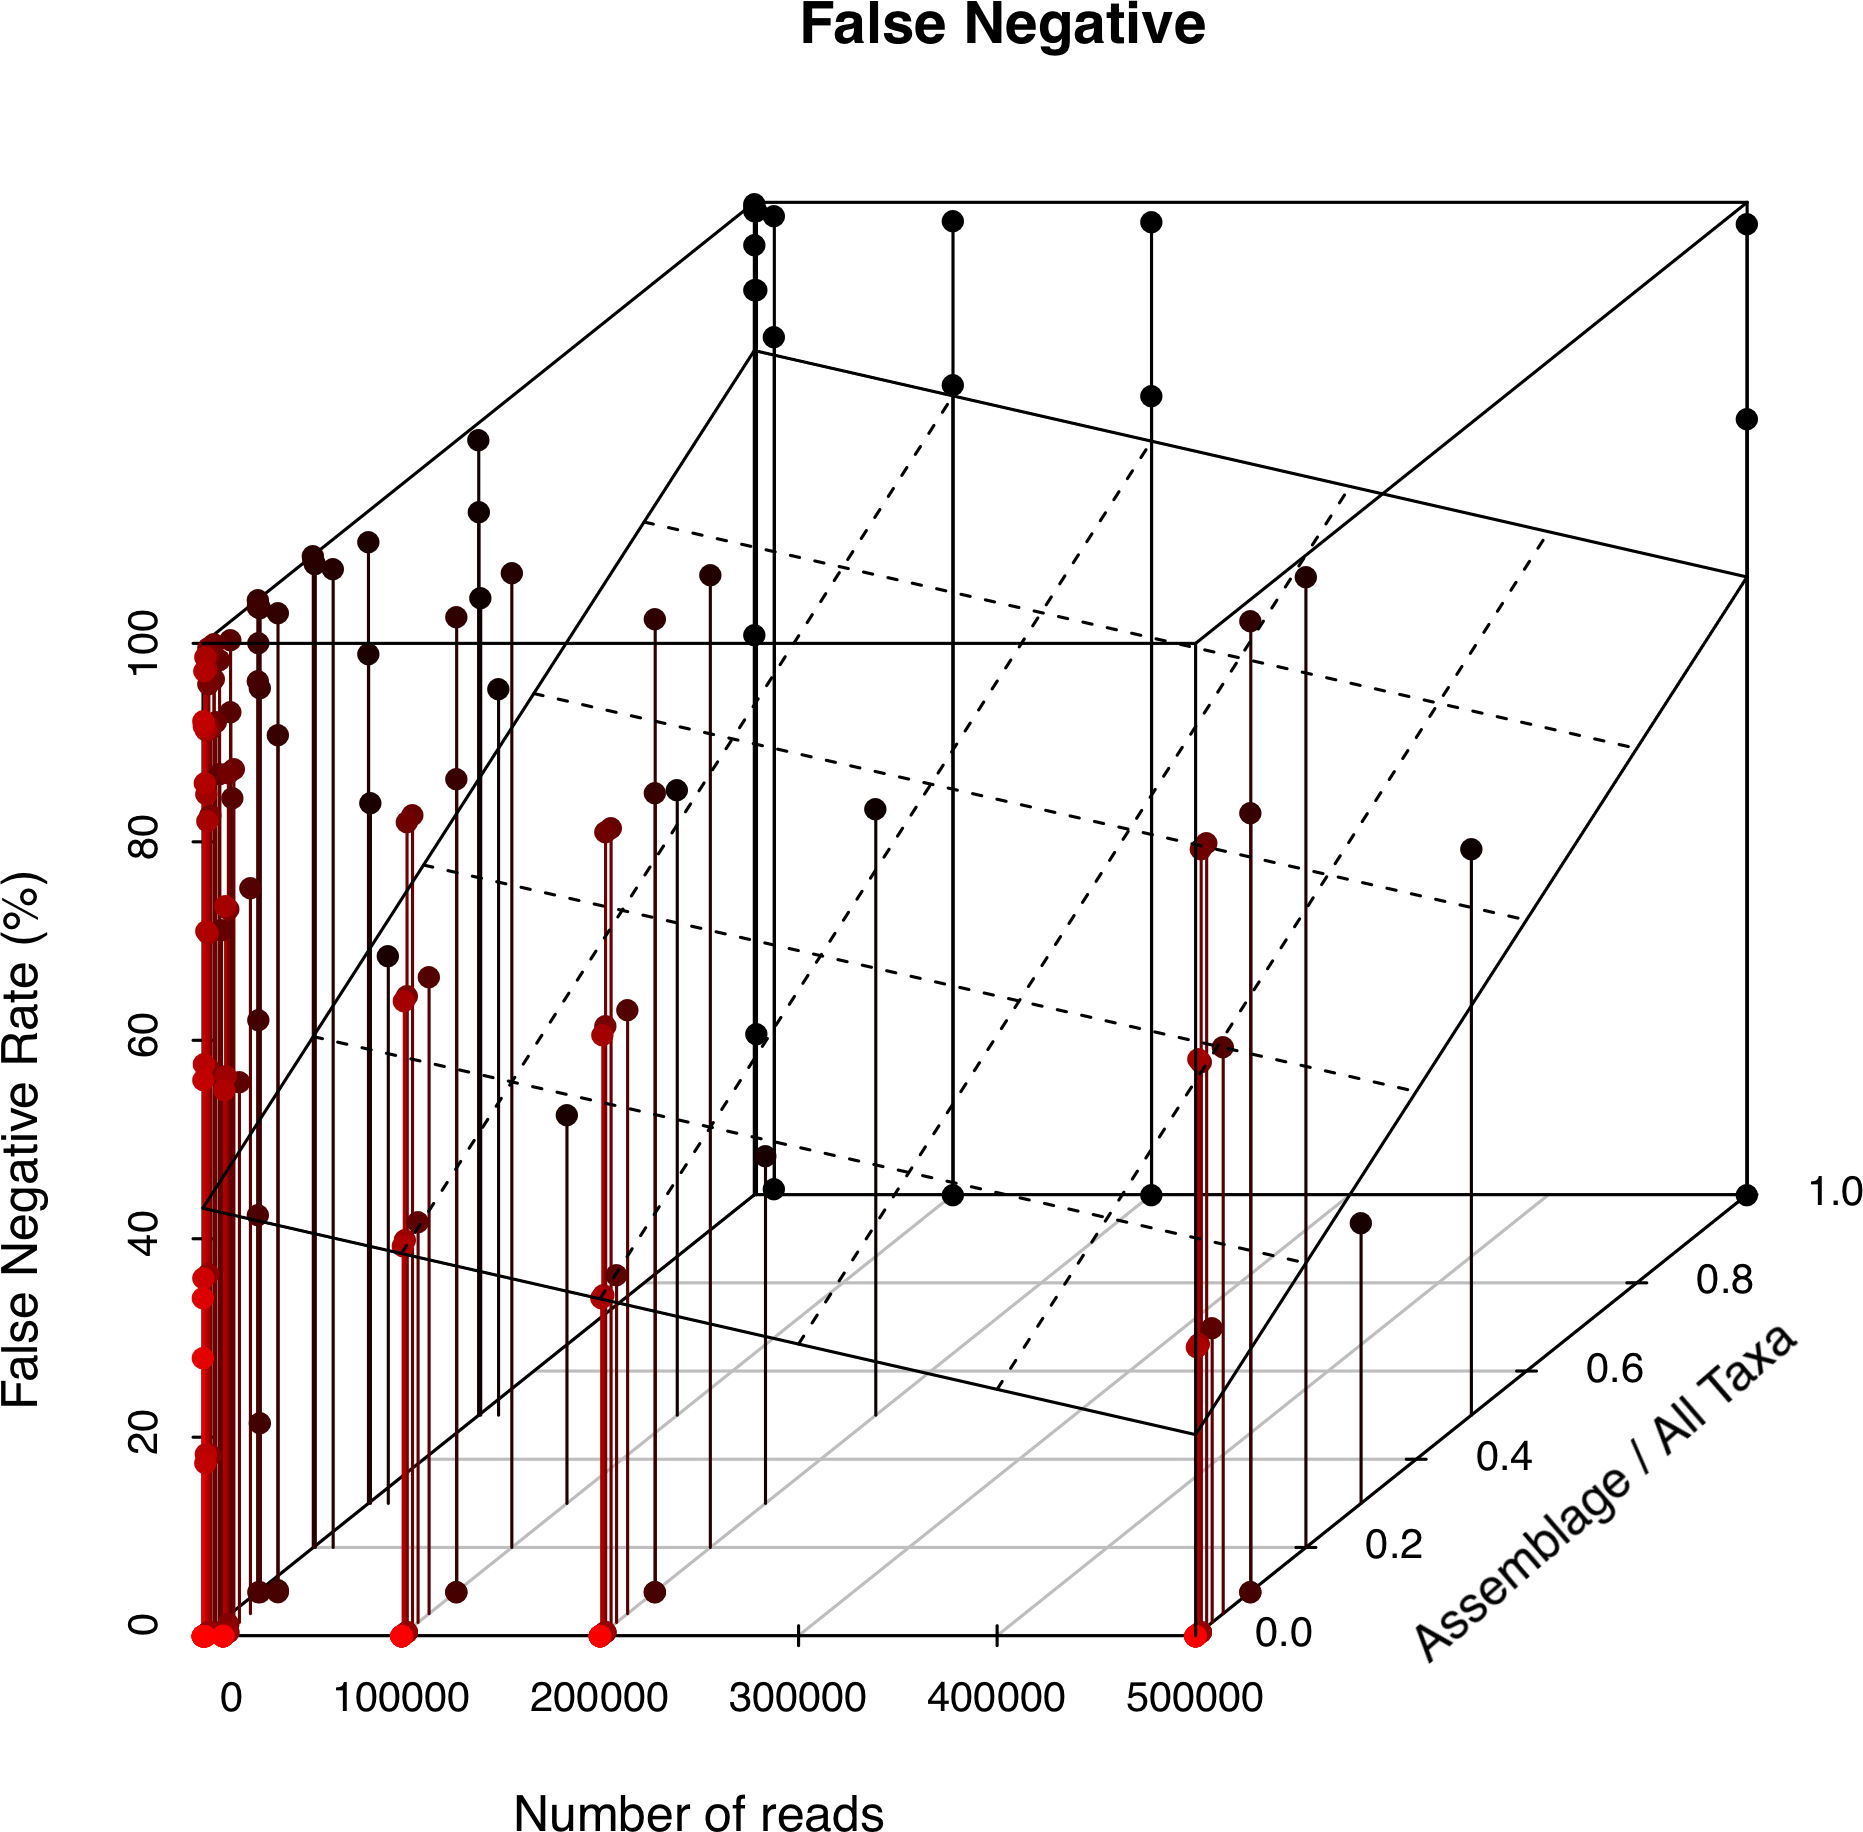
\includegraphics[width=0.45\textwidth]{../minspec/falsenegative.png}
}

&
%\quad %add desired spacing between images, e. g. ~, \quad, \qquad etc. 
%(or a blank line to force the subfigure onto a new line)

\subfloat[\sffamily{}\softwarename{minspec}-attributable false negative rate (\%) --- the percentage of \acp{OTU} not in the assemblage that generated \softwarename{blast} hits but were incorrectly removed by \softwarename{minspec}.\label{fig:minspecvalidationminspecfalsenegative}]{
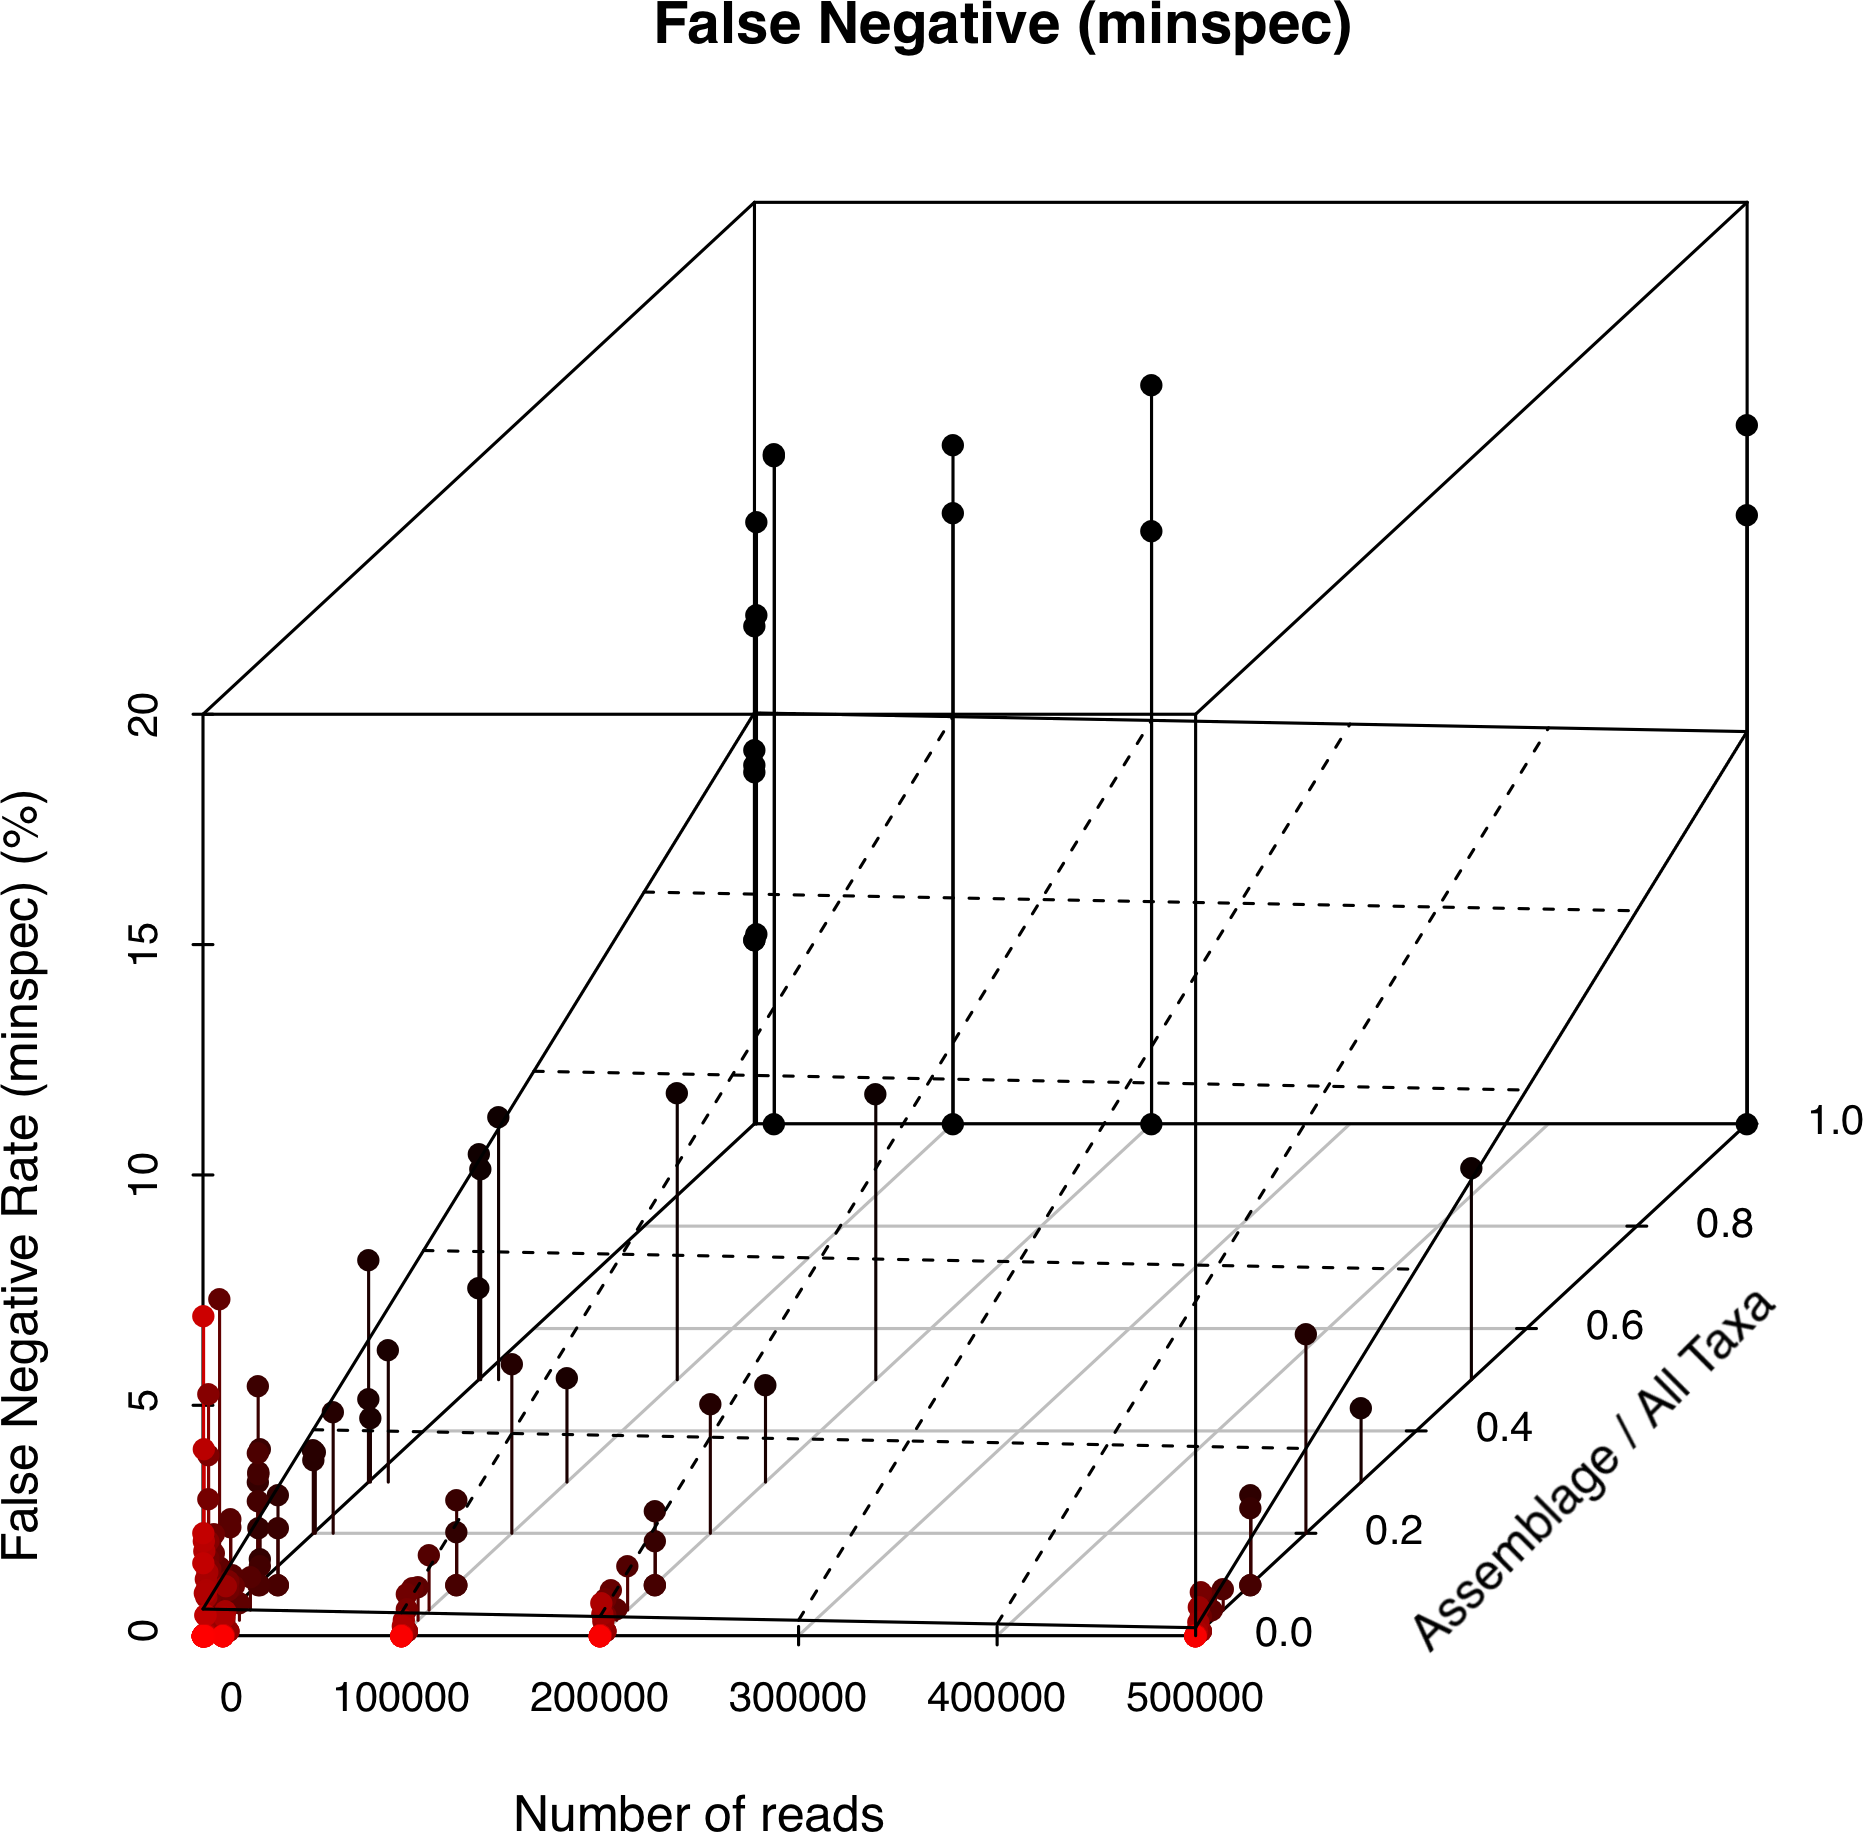
\includegraphics[width=0.45\textwidth]{../minspec/minspecfalsenegative.png}
}
\bigskip
\\
\bigskip
\\
%\quad %add desired spacing between images, e. g. ~, \quad, \qquad etc. 
%(or a blank line to force the subfigure onto a new line)

\subfloat[\sffamily{}False positive rate (\%) --- the percentage of \acp{OTU} not in the assemblage that were present in the \softwarename{blast} results following \softwarename{minspec} processing. \label{fig:minspecvalidationfalsepositive}]{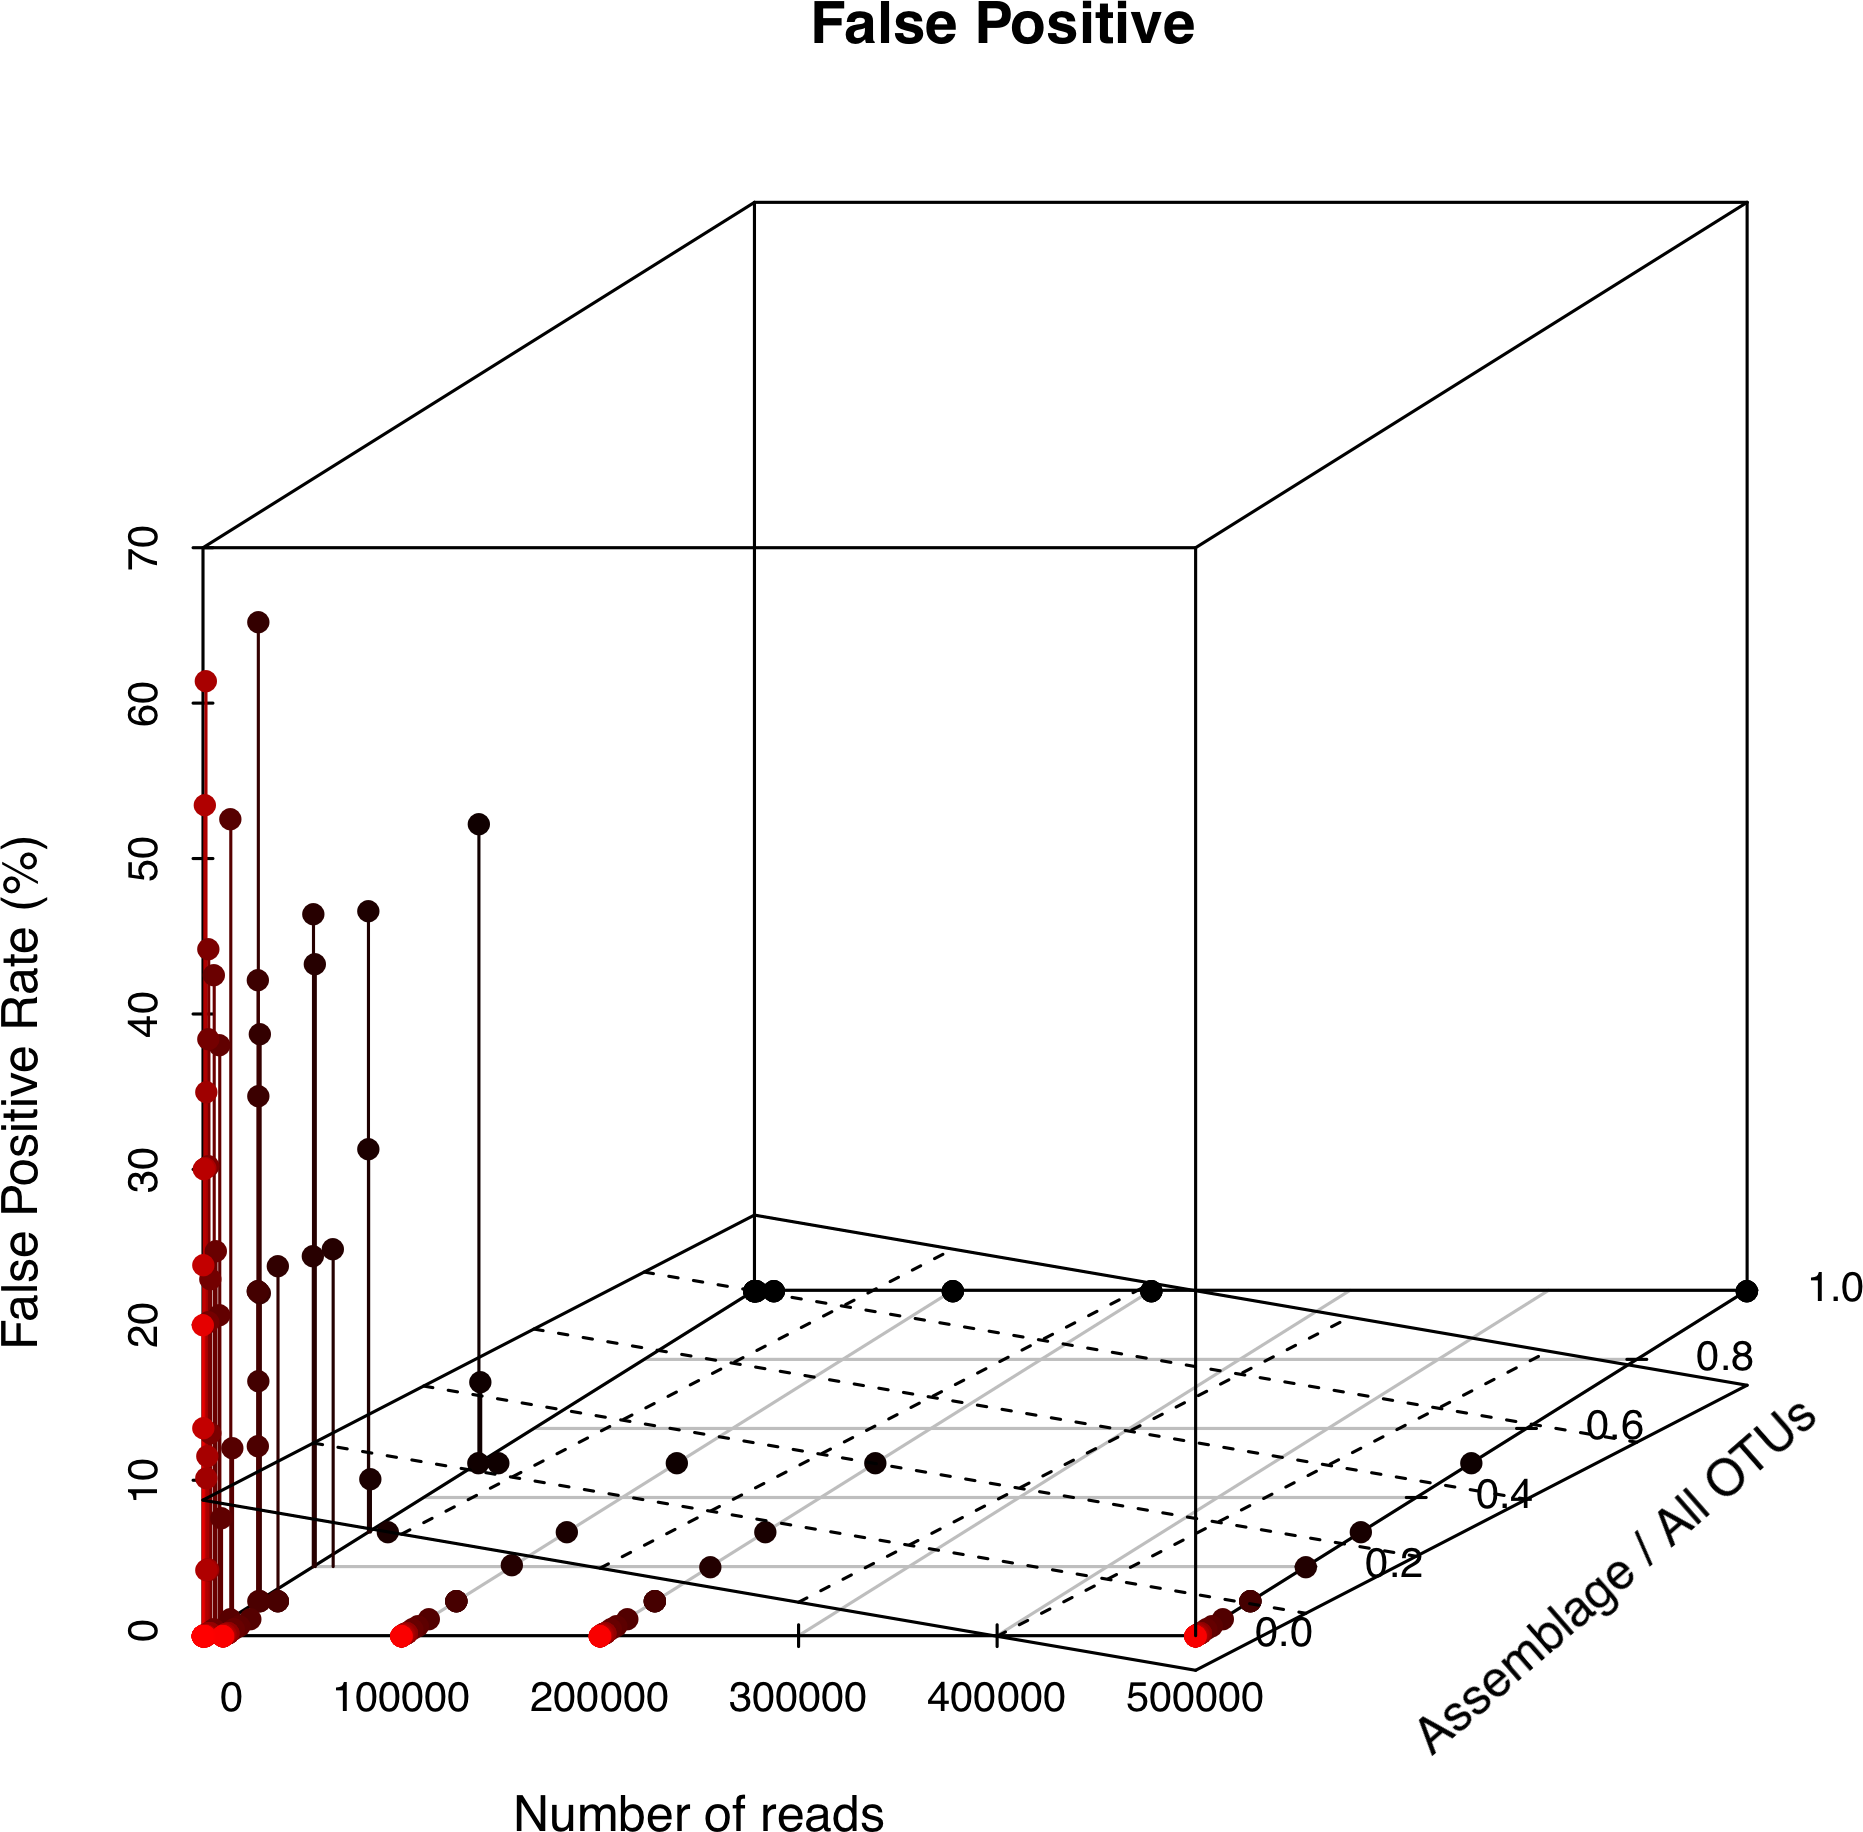
\includegraphics[width=0.45\textwidth]{../minspec/falsepositive.png}}

&
%\quad %add desired spacing between images, e. g. ~, \quad, \qquad etc. 
%(or a blank line to force the subfigure onto a new line)

\subfloat[\sffamily{}Proportion of false \acp{OTU} --- \acp{OTU} that were not part of the simulated assemblage but which generated hits due to simulated sequence identity --- that were correctly identified and removed by \softwarename{minspec}.\label{fig:minspecvalidationfalseotusaremoved}]{
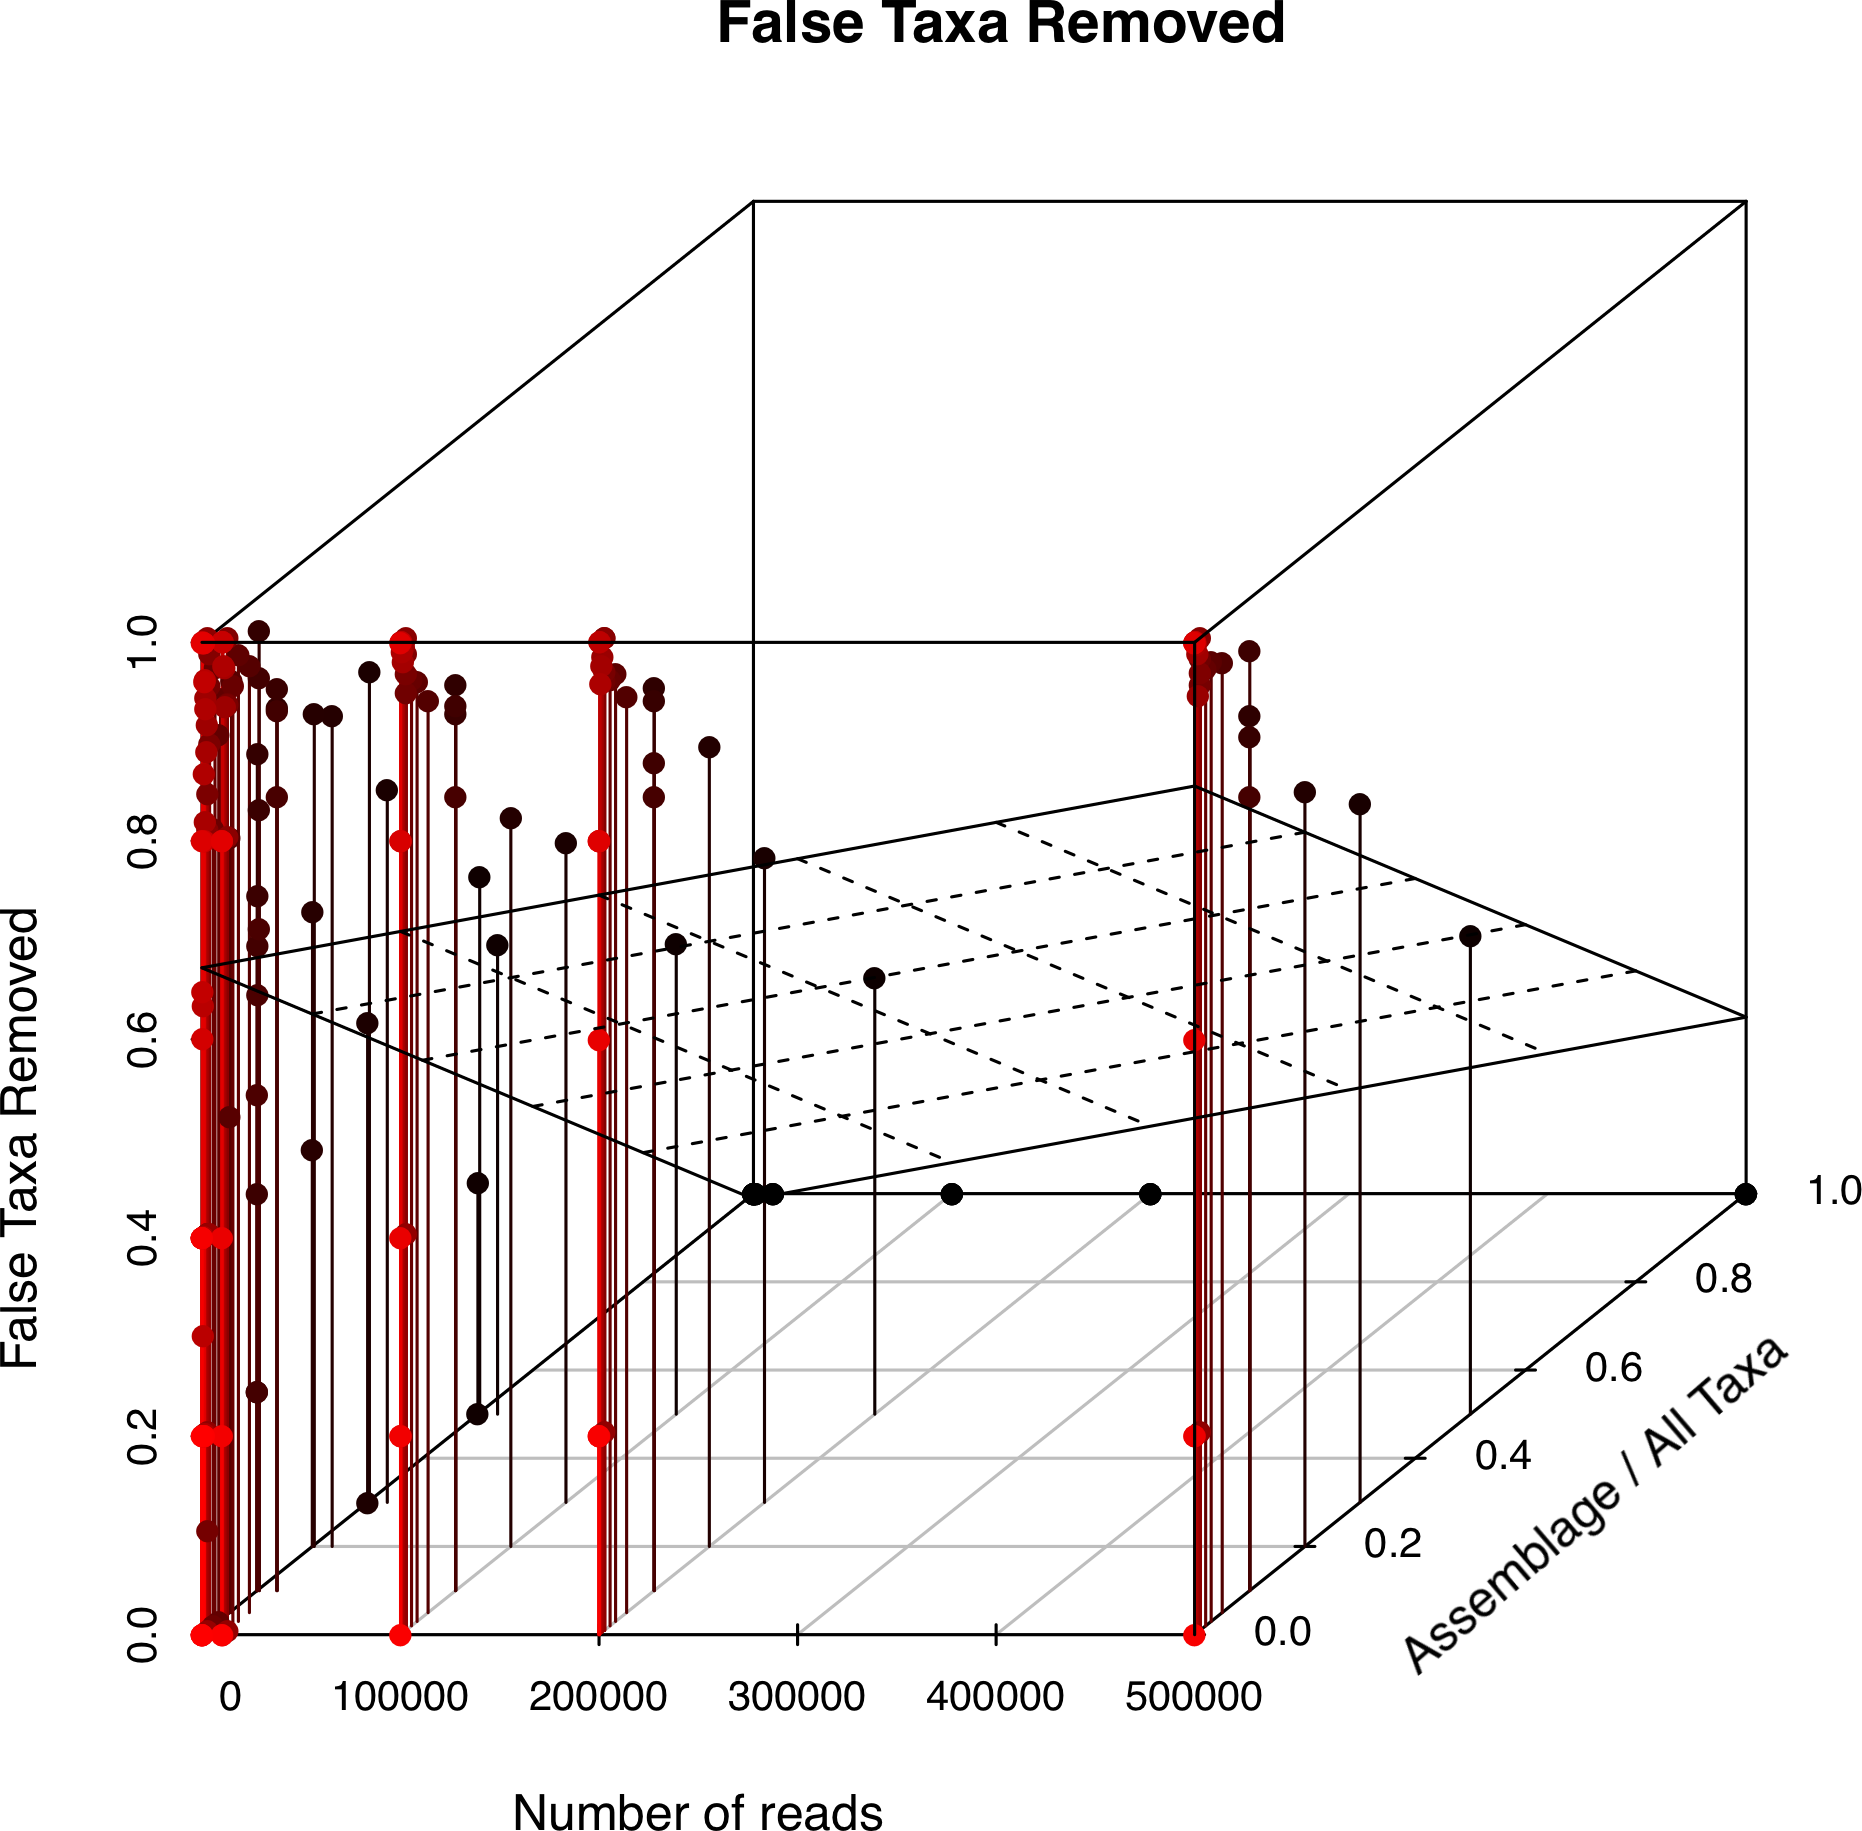
\includegraphics[width=0.45\textwidth]{../minspec/falseotusremoved.png}
}
\\

\end{tabular}

\caption[Results of \softwarename{minspec} validation]{Results of repeated trials of \softwarename{minspec} on simulated metagenomic studies with multiple permutations of parameters (number of reads, number of simulated \acp{OTU}, size of simulated assemblage).
The number of simulated \acp{OTU} and size of simulated assemblage are represented as a ratio on the z-axis (``assemblage / all \acp{OTU}'').
Each permutation was repeated five times.
A plane representing a linear regression has been overlaid on each plot to indicate the trend.
Points have been tinted to aid the perception of depth; colour is not otherwise meaningful.
}\label{fig:minspecvalidation}
\end{figure}


\section{Discussion}

The false negative rate, or percentage of \acp{OTU} in the simulated assemblage which were absent from the \softwarename{blast} results following \softwarename{minspec} processing, was generally high, ranging from \textapprox{}20\% under ideal conditions (a low assemblage / all \acp{OTU} ratio, and 500,000-read metagenomic sample) to \textapprox{}90\% in the worst case (a high assemblage / all \acp{OTU} ratio and a small metagenomic sample) \figref{fig:minspecvalidationfalsenegative}.
The assemblage / all \acp{OTU} ratio (hereafter referred to as ``assemblage ratio'') indicates the proportion of simulated \acp{OTU} (``all \acp{OTU}'') that were chosen to form the simulated assemblage.
A higher ratio means that any \ac{OTU} is more likely on average to be part of the assemblage, and thus that any individual failure to detect a \ac{OTU} is an error.
This problem is mitigated with increasing the number of reads, as this makes it less likely that a given \ac{OTU} would go unsampled.
The extreme false negative rates, in some cases 100\%, represent extreme simulated scenarios (e.g.\ an assemblage of 1 \ac{OTU} drawn from a pool of 100,000), and thus do not reflect real metagenomic studies.

Because the majority of false negatives are attributable to undersampling and failure of \acp{OTU} to generate \softwarename{blast} hits --- properties the simulated metagenomic experiments share with real ones --- a second metric, the false negative (\softwarename{minspec}) rate, was calculated \figref{fig:minspecvalidationminspecfalsenegative}.
This is the proportion of \acp{OTU} in the assemblage that generated \softwarename{blast} hits, but were incorrectly removed by \softwarename{minspec}.
This rate thus represents error attributable only to \softwarename{minspec}.
The false negative (\softwarename{minspec}) rate was generally low, ranging from \textapprox{}0--1\% for low assemblage ratios, to \textapprox{}15--20\% under high ratios.
Surprisingly, increasing the number of reads only slightly decreased the rate, at both low and high assemblage ratios.
This suggests \softwarename{minspec} is more affected by the degree of similarities between \acp{OTU} than by undersampling.

The false positive rate, or percentage of \acp{OTU} not in the assemblage which nevertheless generated high-quality \softwarename{blast} matches that were not identified and removed by \softwarename{minspec}, was generally \textapprox{}0--5\% except for extremely small read sets and low assemblage ratios, where it reached as high as 60\% \figref{fig:minspecvalidationfalsepositive}.
These results reinforce the value of larger read sets, and show that once a modest metagenome size is reached (\textapprox{}100,000 reads) very few false positives can be expected.

The proportion of false \acp{OTU} removed was calculated to measure \softwarename{minspec}'s efficacy in identifying and eliminating \ac{OTU} which are not part of the sampled assemblage yet generate high-quality \softwarename{blast} matches.
This rate varied from 0--1 depending on the parameters of the assemblage \figref{fig:minspecvalidationfalseotusremoved}.
For simulations with a low assemblage ratio, the proportion was generally high ($> 0.6$), although there were simulated experiments with a low ratio where the proportion was low or zero.
However, in all simulations with an assemblage ratio of 1, the proportion was 0, and the regression indicated a generally inverse relationship between the ratio and the proportion of false \acp{OTU} removed.
This is likely because in assemblages with a higher assemblage ratio, there are fewer false \acp{OTU} to remove; in assemblages with a ratio of 1, there are none.
The high proportion of false \acp{OTU} correctly identified in simulations with a low assemblage ratio is thus a good indication that \softwarename{minspec} is effective at identifying and removing false \acp{OTU}, especially as this proportion far exceeds the false positive and false negative (\softwarename{minspec}) rates for comparable experiments.
As expected, increasing the number of reads improved \softwarename{minspec}'s accuracy.

\section{Conclusions}

Overall, the simulated experiments validated both the accuracy and usefulness of \softwarename{minspec} as a tool for reducing error in metagenomic studies.
It is worth noting that the assemblage ratio is not an inherent property of an assemblage, although it is limited by the assemblage's \ac{OTU} richness.
Rather, it can be decreased, and thus the accuracy of the metagenomic experiment improved, by performing \softwarename{blast} searches against larger databases with finer taxonomic resolution.
These results thus reinforce the value of both large read sets and comprehensive reference databases in obtaining high-quality metagenomic results.

At the time of writing, \softwarename{minspec} has been used in two published projects: \citet{Wilkins:2012wg} and \citet{Williams:2012gsa}.


%reset acronyms
\glsresetall
\chapter[The Polar Front]{The Polar Front as a major biogeographic boundary in the Southern Ocean} 
\label{ch:polarfront}

\previouslypublished{Sections of this chapter have been previously published in \bibentry{Wilkins:2012wg}.}

\section{Abstract}

The \ac{PF} is a major oceanographic feature of the \ac{SO}, dividing surface water masses with distinct physicochemical characteristics.
To confirm and characterise the \ac{PF}'s role as a biogeographic barrier in the \ac{SO}, sixteen metagenomic samples were collected on a latitudinal transect from waters near Hobart, Australia (44\textdegree{} S) to near the Mertz Glacier, Antarctica (67\textdegree{} S).
The samples were shotgun sequenced, and the community composition and functional potential of the captured microorganisms were analysed.
The SAR11 and SAR116 clades and the cyanobacterial genera \genus{Prochlorococcus} and \genus{Synechococcus} were strongly overrepresented north of the \ac{PF}.
Conversely, the \ac{GSO-EOSA-1} complex, the phyla Bacteroidetes and Verrucomicrobia and order Rhodobacterales were overrepresented in waters south of the \ac{PF}. 
Functions enriched south of the \ac{PF} included a range of transporters, sulphur reduction and histidine degradation to glutamate, while branched-chain amino acid transport, nucleic acid biosynthesis and methionine salvage were overrepresented north of the \ac{PF}.
The taxonomic and functional characteristics suggested a shift of primary production from cyanobacteria in the north to eukaryotic phytoplankton in the south, and reflected the different trophic states of the two regions. 
Overall, this study supported the \ac{PF} as a defining biogeographic feature of the \ac{SO}.

%reset acronyms
\glsresetall

\section{Introduction}

The surface waters of the \ac{SO} consist of zones separated by circumpolar fronts, the locations of which vary with time and longitude \cite{Whitworth:1980wo,Orsi:1995va,Sokolov:2002tc}.
From north to south, the major fronts are the \ac{STF}, the \ac{SAF} and the \ac{PF} \figref{fig:oceanographymap}.
The \ac{SAF} and \ac{PF} are associated with the \ac{ACC}, the world's largest ocean current and a defining oceanographic feature of the \ac{SO}.
Anthropogenic climate change may be driving the warming and freshening of the \ac{ACC} \cite{Boning:2008il}.
It may also be shifting the \ac{ACC} and associated fronts poleward; the mean path of the current has moved \textapprox{}50 km south since the 1950s \cite{Gille:2002fr}.
If this migration continues, by 2100 it will have displaced a volume of water south of the \ac{ACC} approximately equivalent to the Arctic Ocean \cite{Fyfe:2005vp}.

Climate change may also be affecting the surface regions defined by these fronts.
The major surface zones of the \ac{SO} are the \ac{SAZ}, between the \ac{STF} and \ac{SAF}; the \ac{PFZ}, between the \ac{SAF} and the \ac{PF}; and the \ac{AZ}, between the \ac{PF} and the Antarctic continent \figref{fig:oceanographymap}.
These zones have different physicochemical properties, such as density, salinity, temperature and nutrient concentrations \cite{Sokolov:2002tc}, and the fronts represent stepwise transitions in these properties \cite{WhitworthIII:1987ky}.
However, as a consequence of climate change, waters on the poleward side of the \ac{ACC} have become warmer and more saline, while those to the north cooler and fresher \cite{Boning:2008il}.

The \ac{PF} has been suggested to be a major biogeographic boundary in the distribution and abundance of both zooplankton \cite{Chiba:2001un,Hunt:2001vp,Esper:2002ui,Ward:2003db} and bacterioplankton \cite{Selje:2004ka,Abell:2005ji,Giebel:2009hr,Weber:2010fi}.
The effects of climate change on the physical oceanography of the \ac{SO} may therefore have global ecological significance, particularly as the \ac{SO} is a major site for sequestration of anthropogenic \ce{CO_{2}} \cite{Sabine:2004fz,MikaloffFletcher:2006ct} through both physicochemical processes and the microbe-driven ``biological pump'' of \ce{CO_{2}} fixation \cite{Thomalla:2011hi}, potentially forming a feedback loop \cite{Cox:2000ko}.
However, the microbial assemblages that inhabit the \ac{SO} are generally poorly understood, and their diversity and functional capacity poorly characterised \citep[reviewed in][]{Murray:2007db}.
A community-level understanding is needed to predict the effects of a shifting \ac{ACC} on the distribution, abundance and ecosystem functions of microorganisms.

Large scale metagenome surveys have not previously been performed in the \ac{SO}.
Compared to traditional environmental microbiological methods such as culture-based or DGGE surveys, metagenomic studies are able to offer both deeper (capture of sequence from rare taxa) and broader (larger sample sizes with greater statistical significance) data on the taxonomic makeup and functional capacities of marine microbial communities \citep[e.g.][]{Rusch:2007ez,Angly:2006wf,Dinsdale:2008cd}.
Metagenome sampling is also better suited to large-scale biogeographic studies, as it allows large numbers of samples to be taken across broad spatial and temporal scales with uniform sampling, storage and processing, compared to e.g.\ culture-based methods where technical replicability is more difficult.

This project is part of a metagenomic survey of the \ac{SO} begun in the austral summer of 2006, based on the sampling design of the \ac{GOS} \cite{Rusch:2007ez}.
The \ac{GOS} sampling strategy involves size fractionation of plankton assemblages by passing seawater through a 20 \micron{} prefilter then capturing planktonic biomass on sequential 3.0 \micron{}, 0.8 \micron{} and 0.1 \micron{} filter membranes.
As well as allowing deeper sequencing of metagenomes and thus better representation of low-abundance taxa \cite{Rusch:2007ez}, this approach allows comparison to other samples collected using the \ac{GOS} methods \citep[e.g.][]{Brown:2012gna}.
This study will thus focus on the 0.1--20 \micron{} fraction of the sampled microbial assemblages.

\section{Methods}
\subsection{Sampling and metagenomic sequencing}

Sampling\footnote{Sampling was performed by Jeffrey M. Hoffman and Jeffrey B. McQuaid.} was conducted on board the RSV \emph{Aurora Australis} during \ac{AAD} cruise V3 \ac{CEAMARC} / \ac{CASO} from 13 December 2007--25 January 2008. 
This cruise occupied the SR3 latitudinal transect from waters near Hobart, Australia (\textapprox{}44\textdegree{} S) to the Mertz Glacier polynya, Antarctica (\textapprox{}67\textdegree{} S) within a longitudinal range of \textapprox{}140--150\textdegree{} E.
Sixteen samples were obtained within this range \figref{fig:samplemap}.

% the sample map
\begin{figure}[!ht]
  \centering
  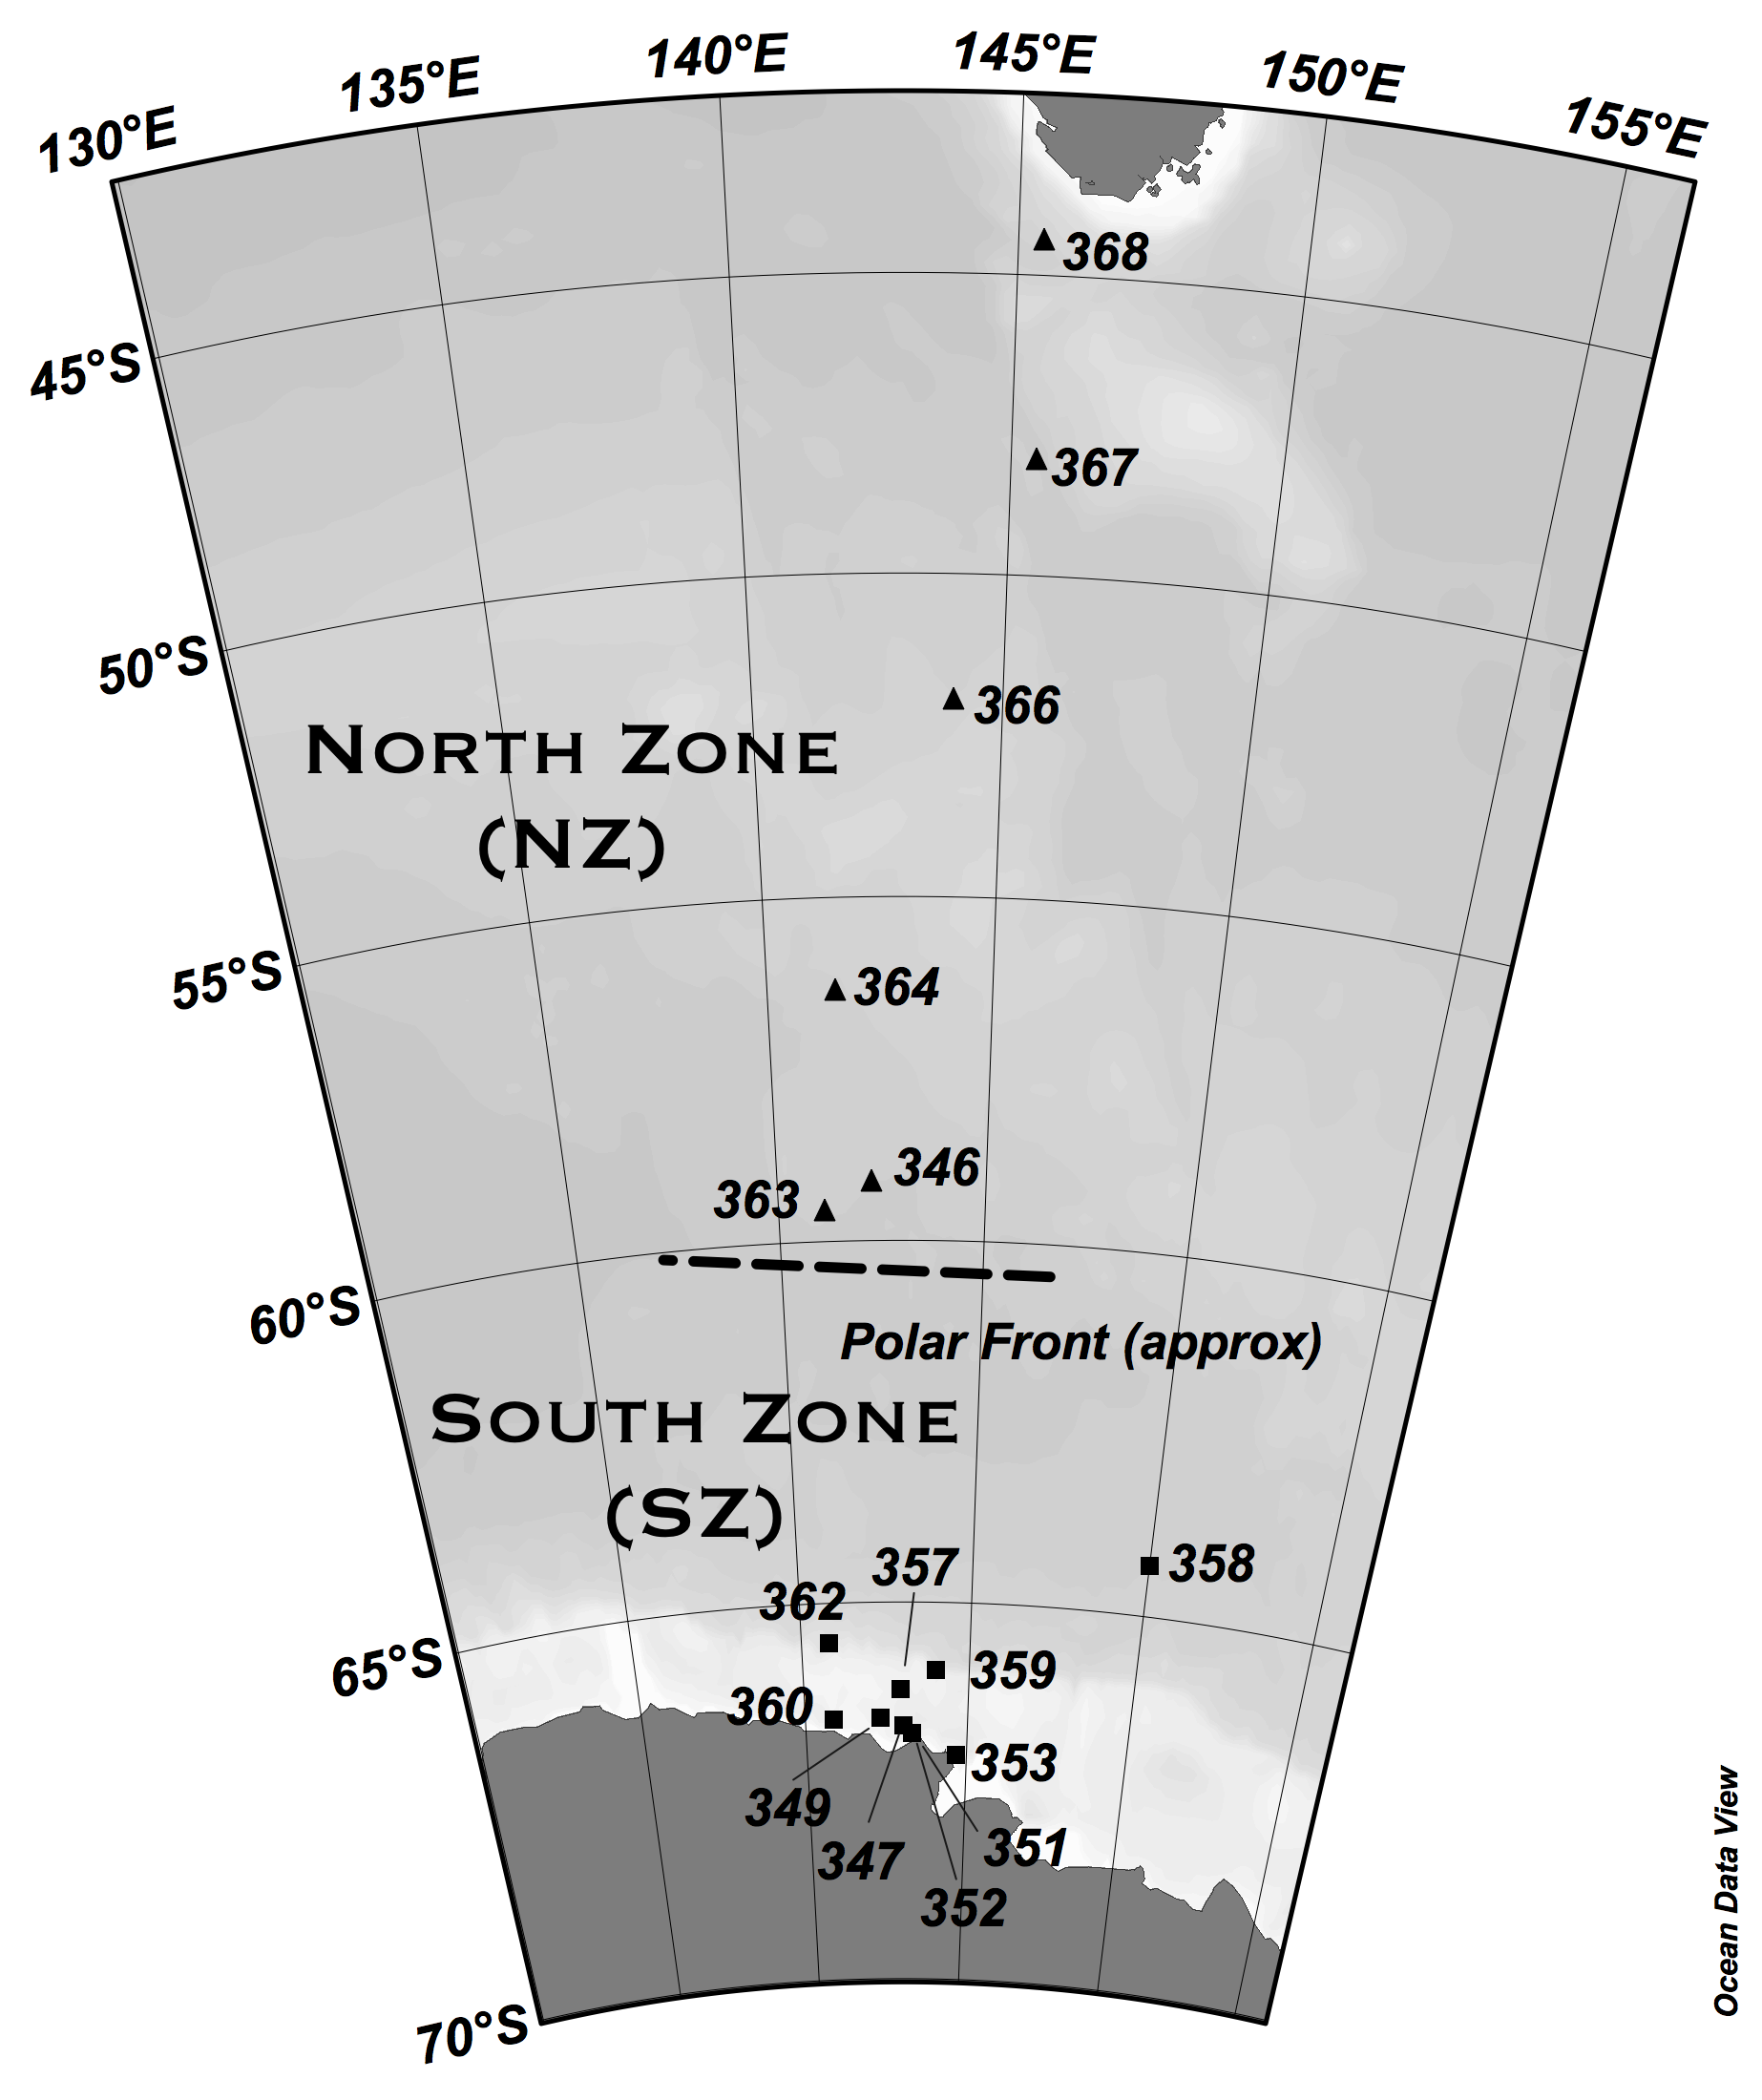
\includegraphics[width=\textwidth]{../polarfront/samplemap.png}
  \caption[Map showing sites of seawater samples used in the Polar Front study]{Sites of seawater samples used in this study. 
  Squares indicate surface samples from the North Zone; crosses samples from the South Zone. 
  The dashed line represents the Polar Front.}
  \label{fig:samplemap}
\end{figure}


A range of physicochemical data were recorded by integrated instruments on the RSV \emph{Aurora Australis} including water column depth, water temperature, salinity, fluorescence and meteorological conditions \tabref{tab:samplelist}.
These data were used to locate the \ac{PFZ} based on a surface temperature gradient of \textapprox{}1.35 \textdegree{}C across a distance of 45--65 km, placing the \ac{PF} at approximately 59.70\textdegree{} S, consistent with previous descriptions \cite{Moore:1999to,Sokolov:2002tc}.
Samples were accordingly grouped into ``North'' and ``South'' zones \tabref{tab:samplelist}.
The \ac{NZ} represents waters from the Subtropical, Subantarctic and \ac{PFZ} regions, while the \ac{SZ} represents the \ac{AZ}.

\begin{sidewaystable}
\sffamily
\caption[Details of samples used in Polar Front study]{\sffamily{}Sampling time, location and physicochemical properties of samples used in this study.
All data were retrieved from underway instruments aboard the RSV \textit{Aurora Australis}.}
\label{tab:samplelist}
\smallskip
\begin{tabularx}{\textheight}{lllXXXXXXXX}
\toprule
\textbf{Sample} & \textbf{Zone} & \textbf{Date} & \textbf{Latitude} & \textbf{Longitude} & \textbf{Water \linebreak Column \linebreak Depth (m)} & \textbf{Sample Depth (m)} & \textbf{Temperature (\textdegree{}C)} & \textbf{Salinity (PSU)} & \textbf{Fluorescence \linebreak (\textmu{}gL\textsuperscript{\textminus{}1})} & \textbf{Volume \linebreak filtered (L)}\\
\midrule

346 & North & 20/12/2007 & \textminus{}59.31 & 142.59 & 4294 & 2 & 2.9 & 33.75 & 0.3 & 500\\
347 & South & 23/12/2007 & \textminus{}66.02 & 142.74 & 450 & 2 & 0.6 & 34.20 & 4.0 & 250\\
349 & South & 27/12/2007 & \textminus{}66.57 & 142.32 & 370 & 1.5 & \textminus{}1.3 & 34.40 & 2.3 & 250\\
351 & South & 28/12/2007 & \textminus{}66.56 & 143.43 & 823 & 1.5 & \textminus{}0.6 & 34.30 & 1.3 & 500\\
352 & South & 29/12/2007 & \textminus{}66.77 & 143.32 & 164 & 2.5 & \textminus{}0.8 & 34.30 & 3.1 & 500\\
353 & South & 30/12/2007 & \textminus{}67.05 & 144.68 & 180 & 2 & \textminus{}1.8 & 34.40 & 0.3 & 500\\
357 & South & 05/01/2008 & \textminus{}66.17 & 143.02 & 580 & 2 & \textminus{}0.4 & 34.15 & 2.5 & 500\\
358 & South & 09/01/2008 & \textminus{}64.30 & 150.03 & 3550 & 2 & 0 & 33.55 & 0.5 & 500\\
359 & South & 12/01/2008 & \textminus{}66.19 & 143.53 & 540 & 2 & \textminus{}0.2 & 34.21 & 2.5 & 500\\
360 & South & 13/01/2008 & \textminus{}66.58 & 141.02 & 316 & 2 & \textminus{}0.7 & 34.04 & 6.2 & 500\\
362 & South & 19/01/2008 & \textminus{}65.54 & 140.83 & 1064 & 2 & 0.7 & 32.20 & 0.5 & 500\\
363 & North & 22/01/2008 & \textminus{}60.00 & 141.31 & 4473 & 2 & 3.3 & 33.77 & 0.1 & 500\\
364 & North & 23/01/2008 & \textminus{}56.70 & 141.88 & 3693 & 2 & 4 & 33.70 & 0.5 & 500\\
366 & North & 24/01/2008 & \textminus{}52.02 & 144.14 & 3180 & 2 & 7.6 & 33.84 & 0.3 & 500\\
367 & North & 25/01/2008 & \textminus{}48.25 & 145.90 & 3490 & 2 & 11 & 34.43 & 0.2 & 500\\
368 & North & 26/01/2008 & \textminus{}44.72 & 145.78 & 3201 & 2 & 14.8 & 34.96 & 1.3 & 560\\

\bottomrule
\end{tabularx}
\end{sidewaystable}


At each station, \textapprox{}250--560 L of seawater was pumped from \textapprox{}1.5--2.5 m below the sea surface into drums stored at ambient temperature on deck. 
Seawater samples were prefiltered through a 20 \micron{} plankton net, then biomass was captured on sequential 3.0 \micron{} 0.8 \micron{} and 0.1 \micron{} 293 mm polyethersulfone membrane filters (Pall, Port Washington, USA), and immediately stored at \textminus{}20 \textdegree{}C \cite{Rusch:2007ez,Ng:2010cd}.

DNA extraction\footnote{DNA extraction was performed by Cynthia Andrews-Pfannkoch and others at the J.\ Craig Venter Institute.} was performed at the J.\ Craig Venter Institute (Rockville, USA) using a modified phenol-chloroform method as described in \citet{Rusch:2007ez}.
Shotgun sequencing was performed on a GS20 FLX Titanium platform (Roche, Branford, USA) also at the J.\ Craig Venter Institute as described in \citet{Lauro:2010jna}.
Perfect duplicate reads were removed using sffToCa (Celera Corporation, Alameda, USA),  read ends were trimmed with \softwarename{Lucy} \cite{Chou:2001ck}, and the bottom 8\% and top 3\% of reads ordered by length were removed as described in \citet{Lauro:2010jna}\footnote{Read quality filtering was performed by Federico M.\ Lauro and Matthew Z.\ DeMaere.}.

\subsection{Phylogenetic analysis of metagenomic data}

\subsubsection{\softwarename{blast} comparison to RefSeq database}

A subset of the RefSeq microbial (bacterial and archaeal) genome database (release 41, retrieved 31 May 2010 from \url{ftp://ftp.ncbi.nih.gov/refseq/release/}) was prepared by excluding sequences with the words ``shotgun'', ``contig'', ``partial'', ``end'' or ``part'' in their headers.
This is necessary to ensure only full and complete genomes yielded matches, as the \ac{GAAS} software tool used for later processing uses this assumption to estimate environmental genome sizes \citep[following][]{Angly:2009ip}.

The metagenomic reads from each sample were compared against this database using \softwarename{tblastx}, with default parameters except for: E-value threshold $1.0\times{}10^{-3}$, cost to open gap 11, cost to extend gap 1, masking of query sequence by \softwarename{SEG} masking with lookup table only.
\acp{OTU} in this study are thus defined as the best species match in RefSeq by these parameters.
The outputs of all \softwarename{tblastx} searches against RefSeq were processed by \softwarename{minspec}, and hits not belonging to the minimal \ac{OTU} sets were removed.

\subsubsection{OTU abundances and variance between zones}

The relative \ac{OTU} abundances for each sample were determined using the \softwarename{perl} script \ac{GAAS} \cite{Angly:2009ip}.
\ac{GAAS} estimates the relative abundance of \acp{OTU} from the number and quality of \softwarename{blast} matches (``hits'') to each \ac{OTU}, taking into account differences in genome size. 
This approach takes advantage of all sequencing reads in a shotgun metagenome, in contrast with marker-gene bases approaches (e.g.\ 16S), and allows relative abundances to be estimated on a ``one genome per cell'' basis, increasing the accuracy of these estimates.
\ac{GAAS} was run with the default settings. 
To normalise for reads which did not yield acceptable hits, the relative abundances for each sample were scaled by that sample's effective \softwarename{blast} hit rate.

A difficulty with the size fractionation approach is that relative abundances cannot be summed across fractions.
This is because each fraction almost certainly represents a different absolute number of cells.
If the relative abundances are summed, the apparent abundance of some \acp{OTU} could be distorted (visually demonstrated in \figreft{fig:fractionabundances}).
Thus, an \ac{OTU} profile was generated for each sample by encoding the scaled relative abundance of each \ac{OTU} from each size fraction as a separate variable.
This allows samples to be compared on the basis of community composition without introducing systematic biases.

\begin{figure}
\centering
\subfloat[\sffamily\label{fig:fractionabundancescellcount}]{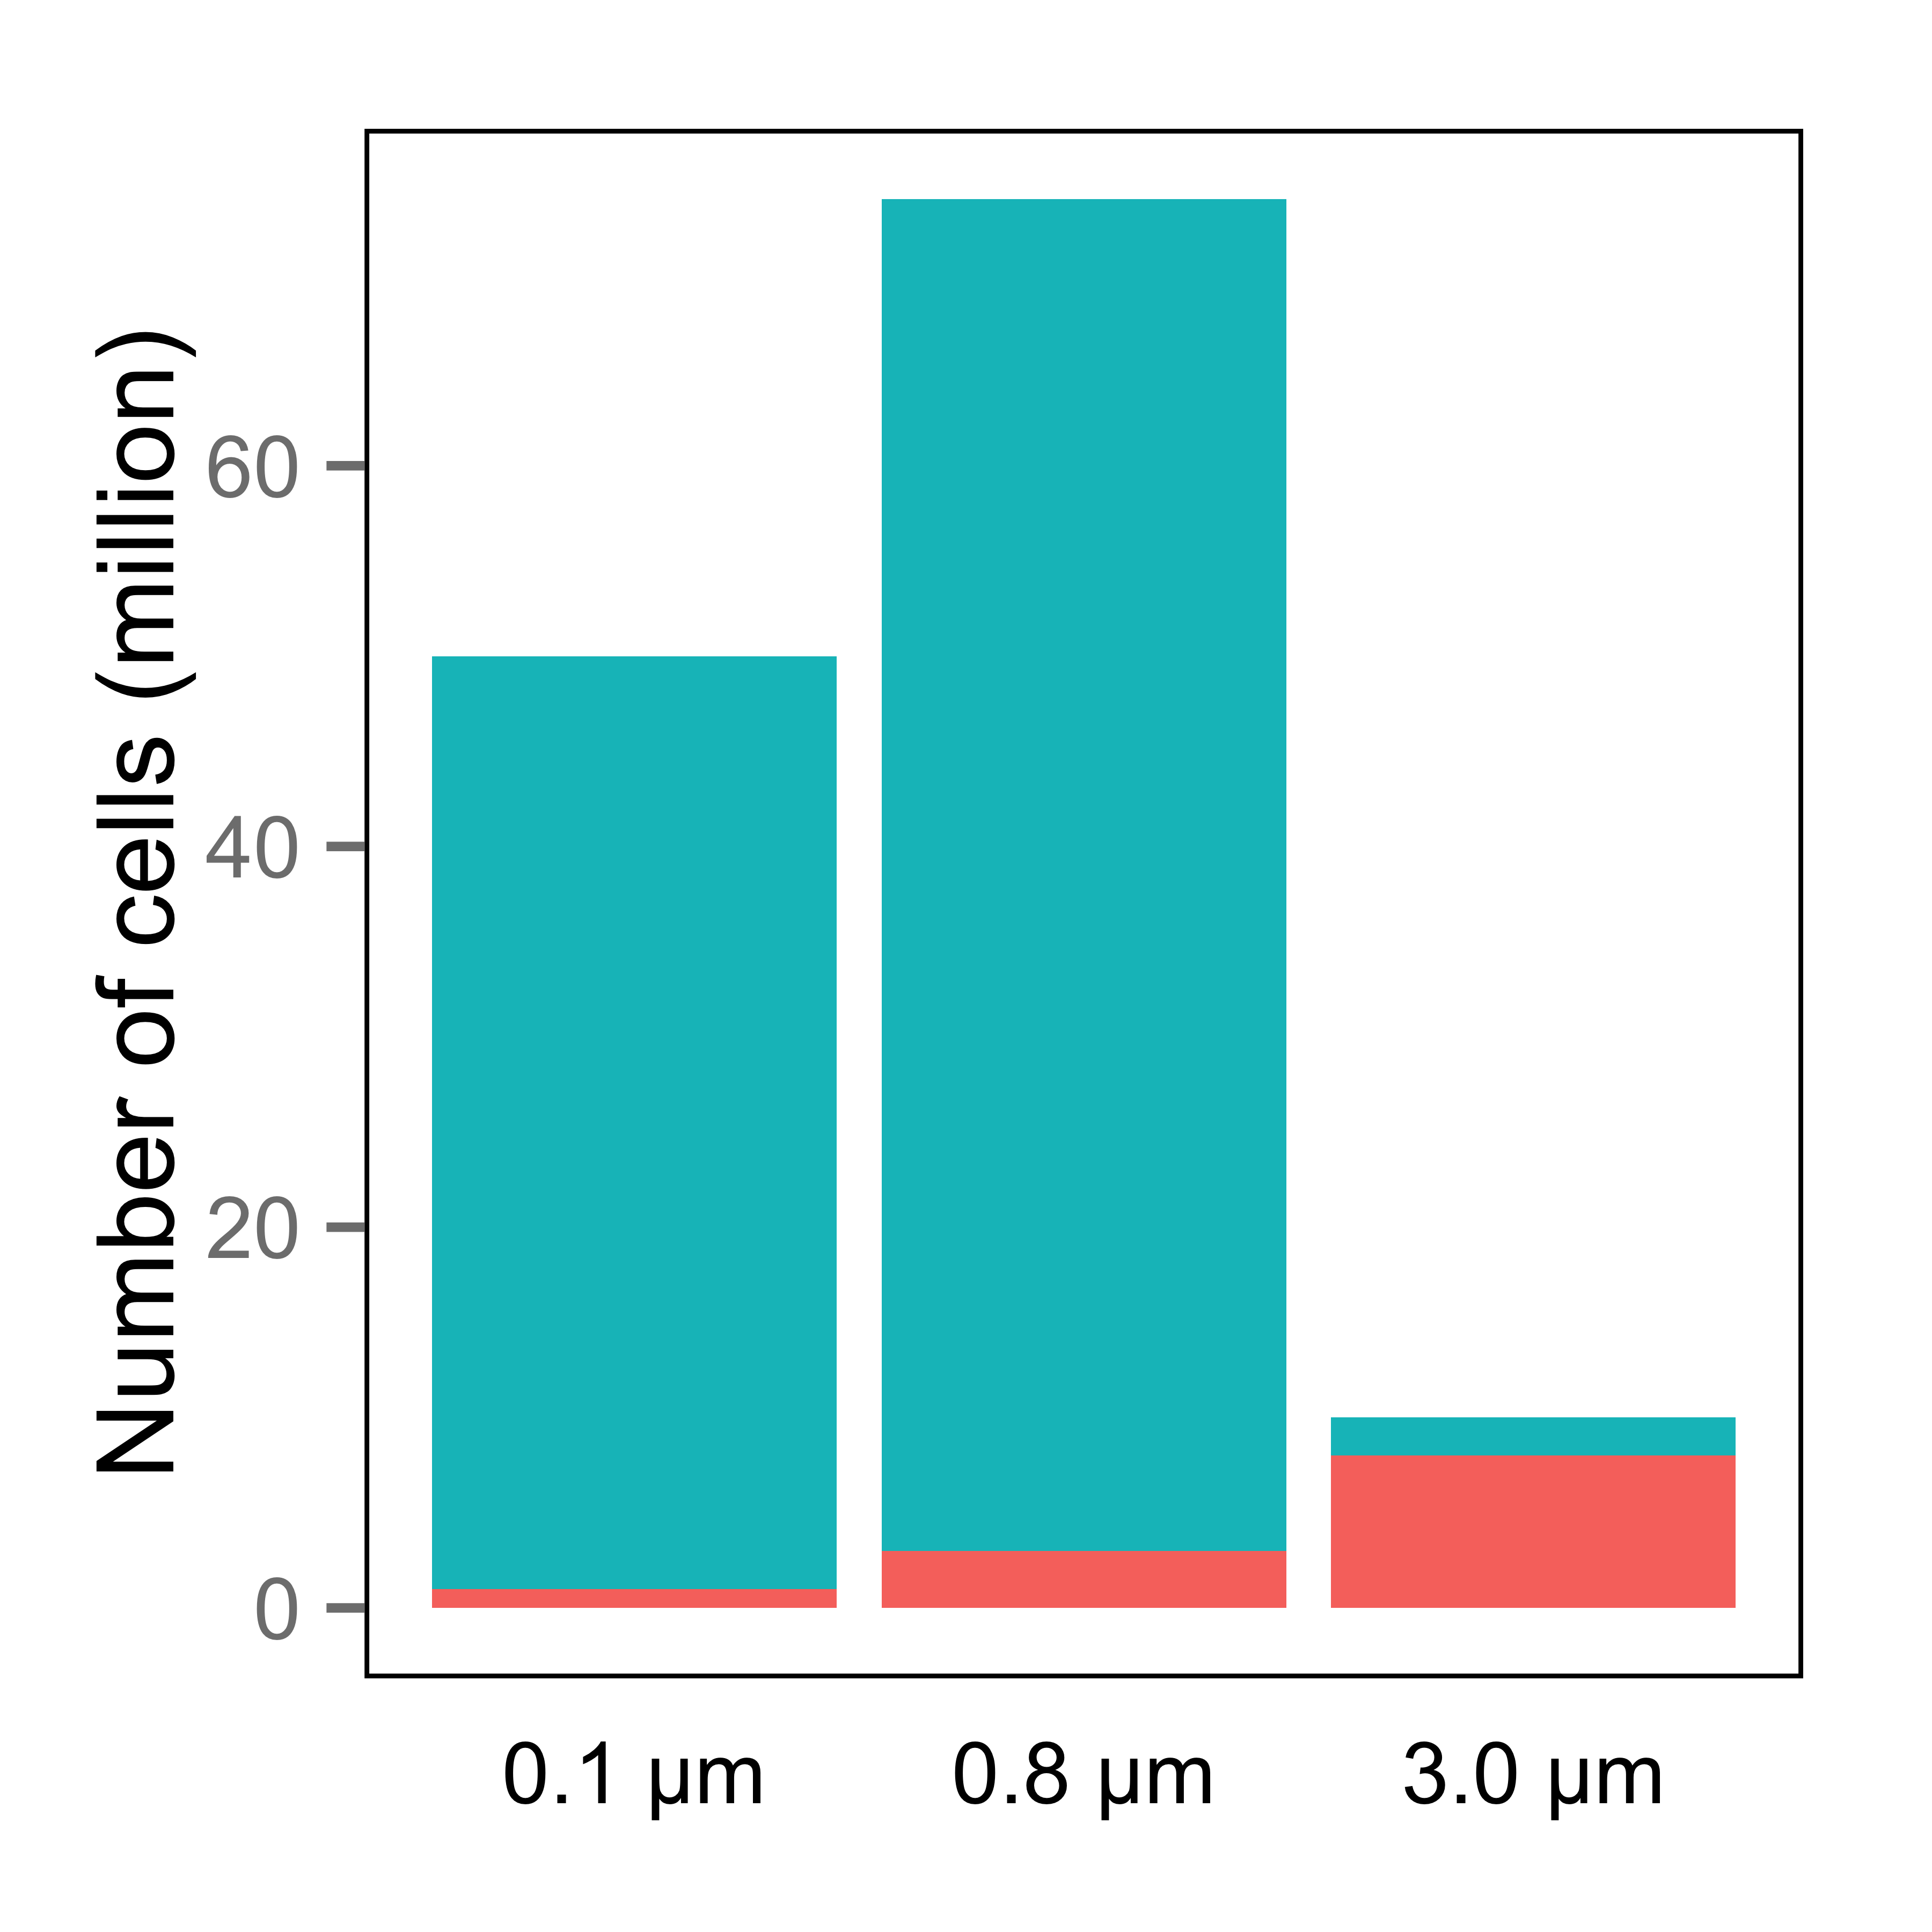
\includegraphics[scale=0.04]{../polarfront/fractionabundances1.png}}
\quad
\subfloat[\sffamily\label{fig:fractionabundancesrelative}]{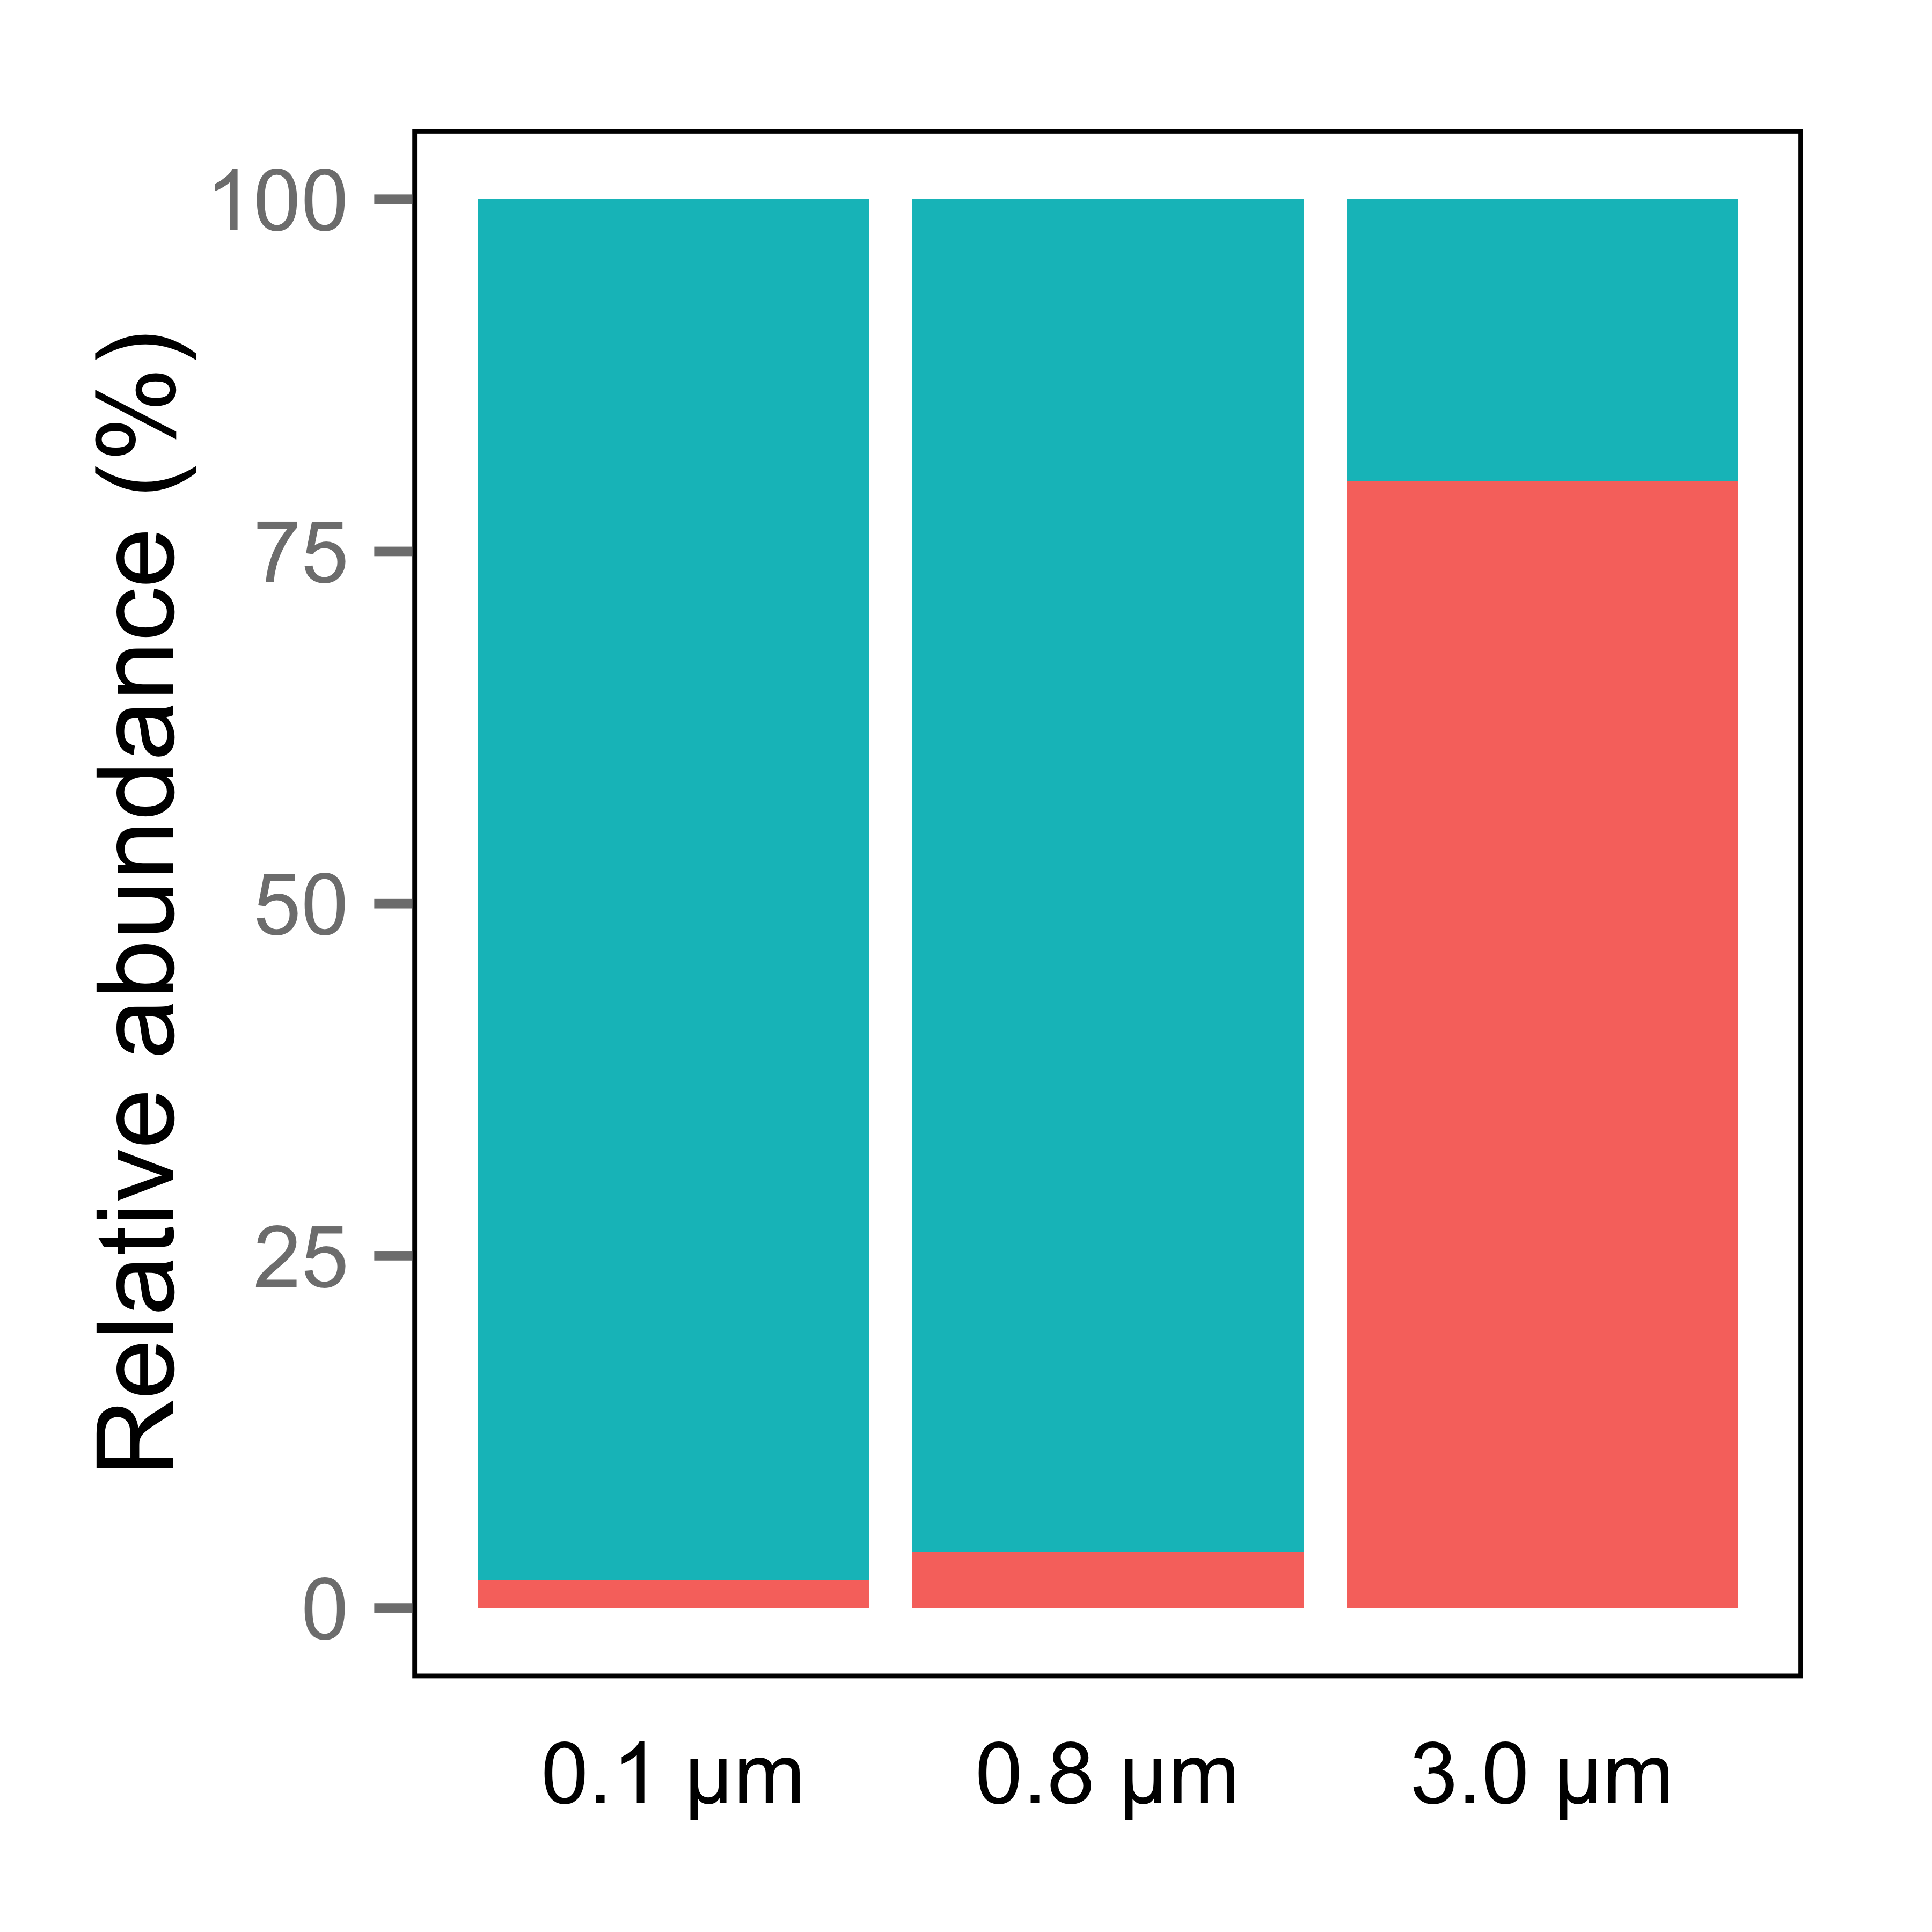
\includegraphics[scale=0.04]{../polarfront/fractionabundances2.png}}
\quad
\subfloat[\sffamily\label{fig:fractionabundancescombined}]{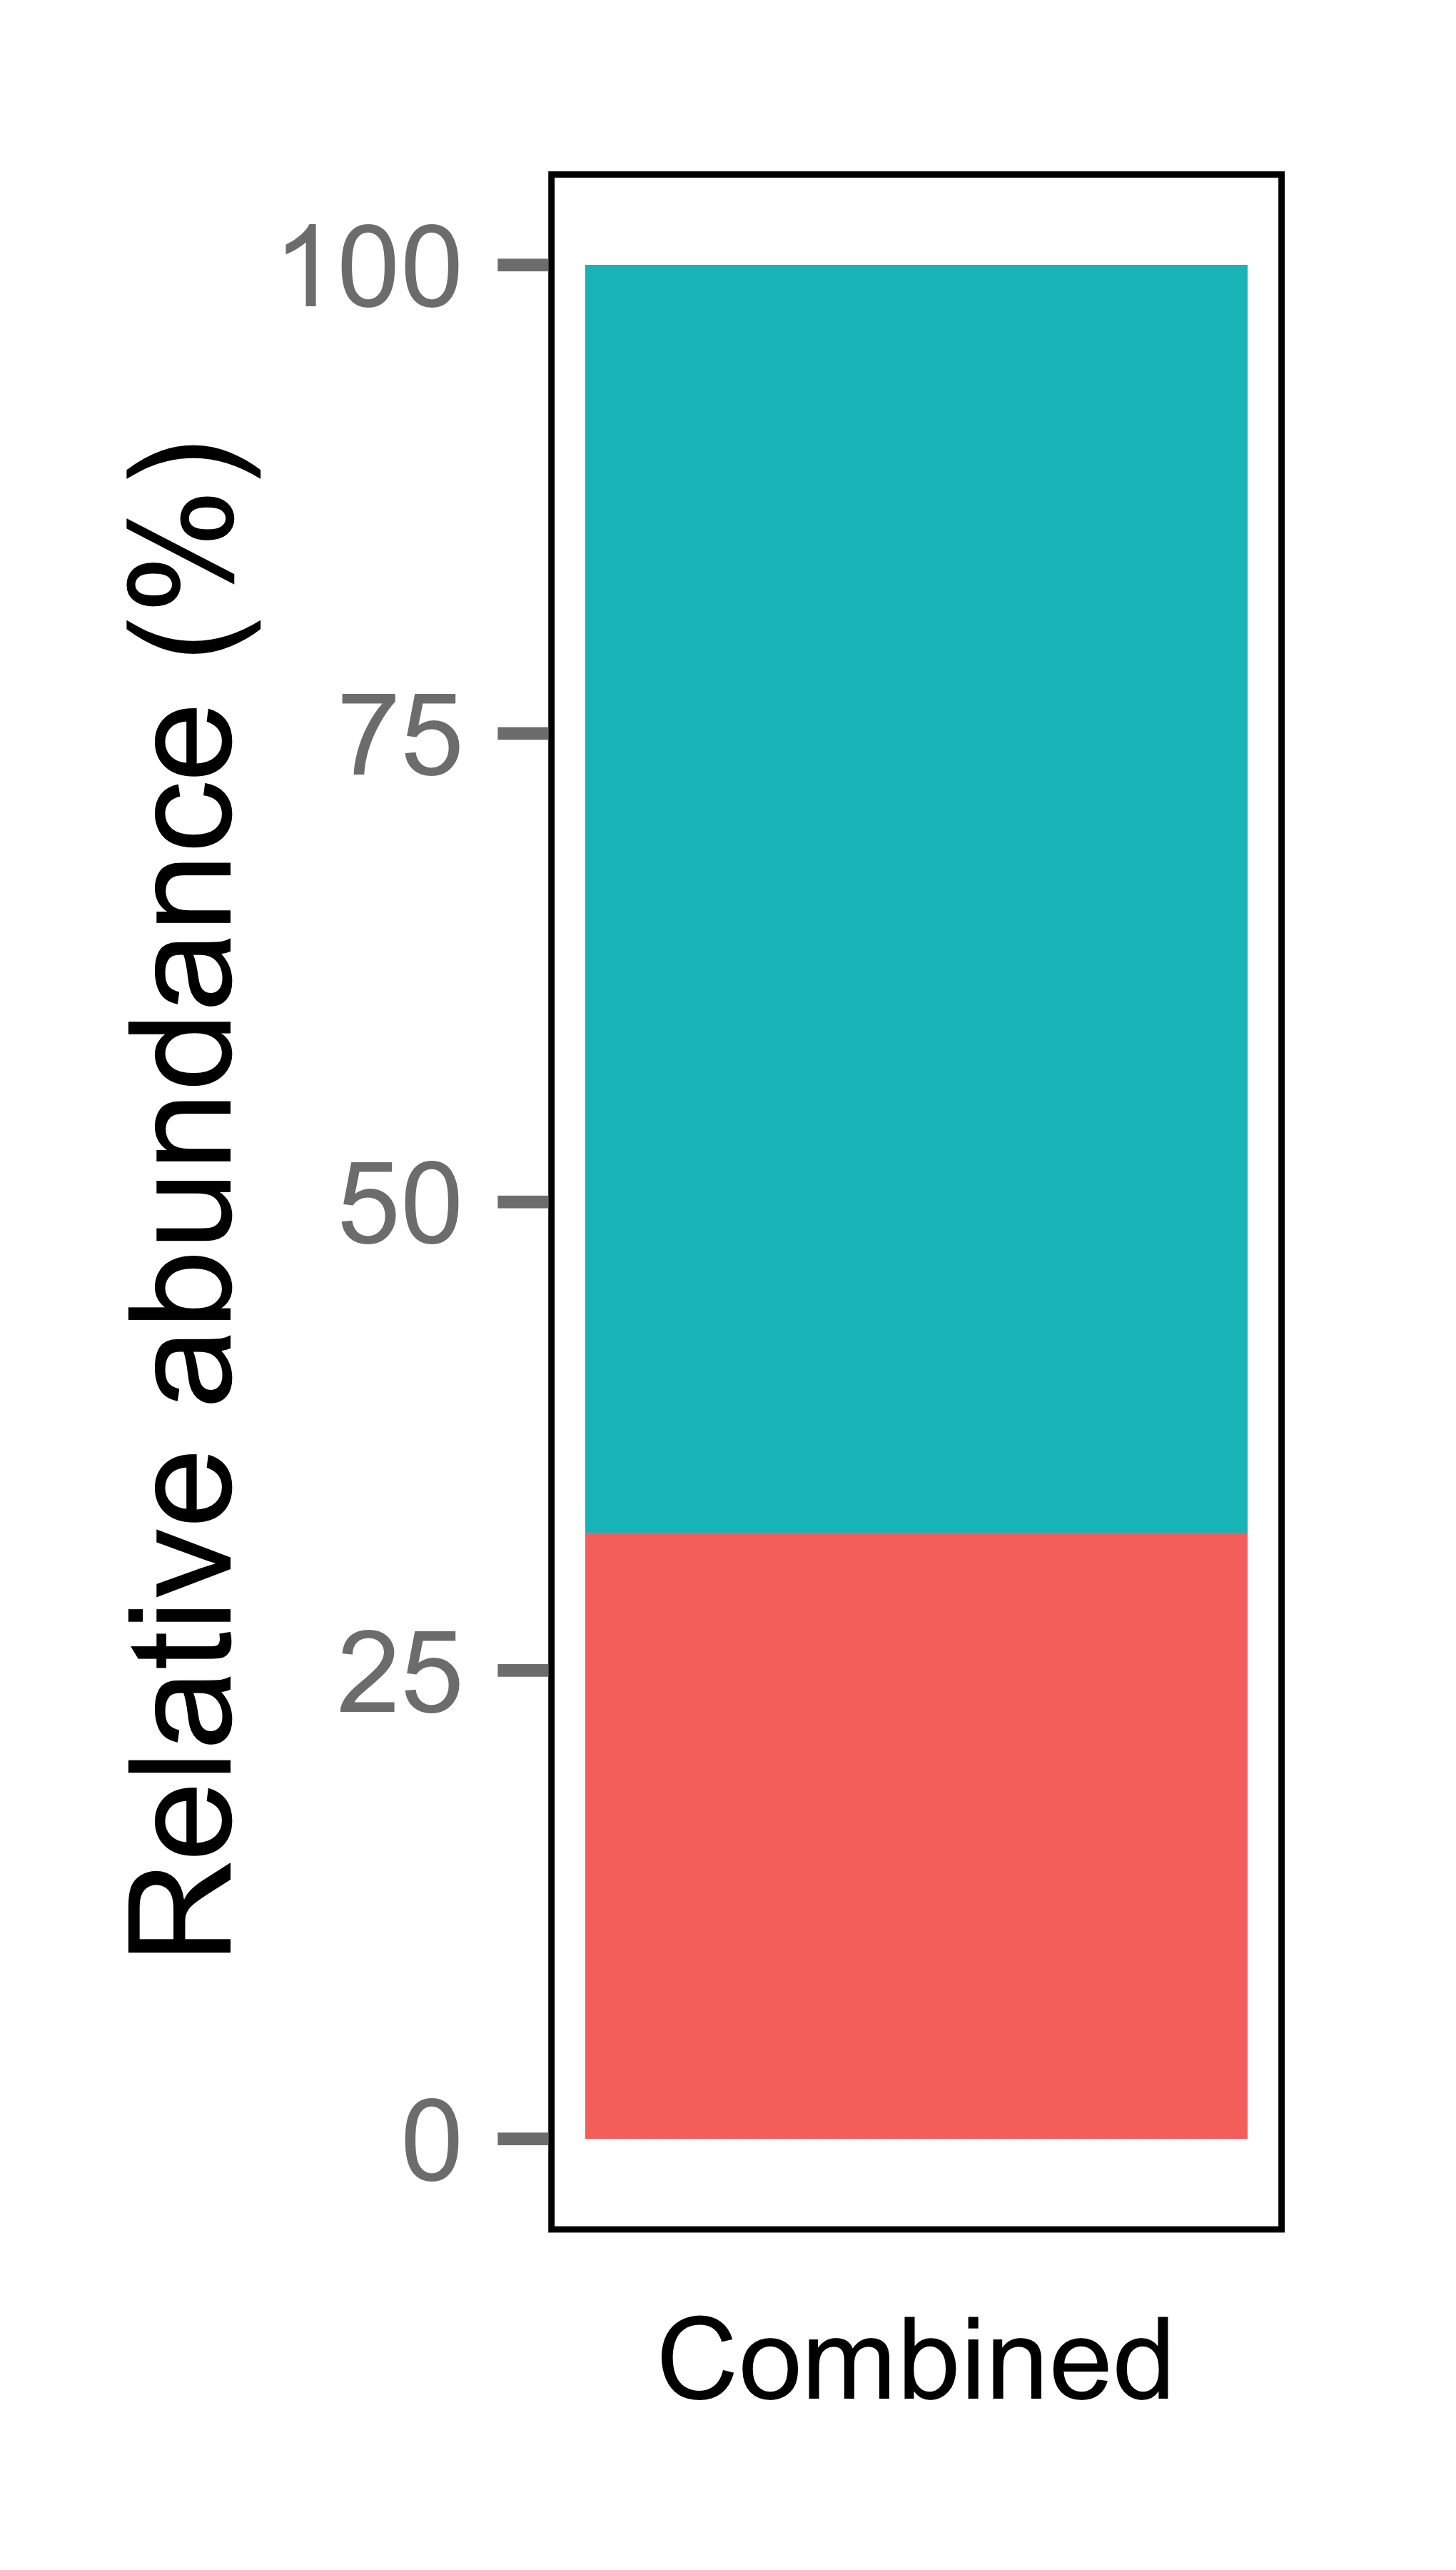
\includegraphics[scale=0.04]{../polarfront/fractionabundances3.png}}
\caption[Summing relative abundances across size fractions]{An example of distortion introduced by summing OTU relative abundances across size fractions. The red OTU composes only 15\% of the \emph{absolute} number of cells captured (a). However, it has a high \emph{relative} abundance (80\%) in the 3.0 \micron{} fraction (b). A metagenomic analysis without cell counts for each size fraction is only able to determine these relative abundances. If the relative abundances for each fraction are simply summed, the red OTU appears to compose 32\% of the community, more than twice the correct value (c). Without cell counts for each fraction, relative abundances cannot be summed between the fractions.}
\label{fig:fractionabundances}
\end{figure}


To test the hypothesis that the oceanic zones harbour significantly different communities, \ac{ANOSIM} with 999 permutations was performed on a standardised, log-transformed Bray-Curtis resemblance matrix of \ac{OTU} profiles.
\ac{SIMPER} analysis was performed to identify the contribution of individual \acp{OTU} to differences between the zones. 
All statistical procedures were performed in \softwarename{PRIMER 6} as described by \citet{Clarke:2001ut}.

\subsubsection{Fragment recruitment to verify \ac{OTU} identification}
Fragment recruitment to reference genomes was visualised as a precaution against unintended sequencing bias and to ensure the \ac{OTU} annotation pipeline was functioning as intended.
Plots of read recruitment depth on reference genomes were generated using a custom script in \softwarename{r} and \softwarename{perl}\footnote{This script, along with other accessory scripts used in this project, is open source and available at \url{https://github.com/wilkox/blast-tools}.}.
Samples from both the \ac{SZ} and \ac{NZ} were randomly selected and their 0.1 \micron{} fractions used as sources of recruited reads.
Three high-abundance and three low-abundance \acp{OTU} were randomly selected as the reference genomes.
As shotgun sequencing of a metagenome should be essentially random, it was predicted that these plots would show fairly even coverage of the reference genomes.
Genomes where all recruited reads were concentrated in a few small regions would be likely candidates for \acp{OTU} which were not present, but shared a small genomic region with an \ac{OTU} which was present, or possibly indicative of non-random priming during shotgun sequencing.

\subsubsection{Additional samples to test ``polynya hypothesis''}
Because many samples from the \ac{SZ} were taken in the region of the Mertz Glacier polynya, an alternative hypothesis for any difference observed between the \ac{SZ} and \ac{NZ} would be that the difference represented the effect of the polynya, rather than the \ac{PF}.
To test this, metagenomes from an additional set of samples collected\footnote{Collection was performed by Ricardo Cavicchioli, Federico M.\ Lauro and Mark V.\ Brown.} in a different project were obtained.
These samples were obtained in waters south of the \ac{PF} on different voyages and in a different longitudinal range \figref{fig:additionalsamples}, where the influence of the Mertz Glacier polynya could not account for any observed difference between the zones.
Sampling, DNA extraction and sequencing were\footnote{TODO who did this?} performed as described above, although only metagenomes from the 0.1--0.8 \micron{} size fraction were available.
The resulting metagenomic reads were compared to RefSeq and weighted relative abundances calculated with \ac{GAAS} as described above.

\begin{table}
\centering
\caption[Additional samples used to test polynya hypothesis]{Dates and locations of additional samples used to falsify the hypothesis that the Mertz Glacier polynya was responsible for the observed biogeographic partitioning.}
\label{tab:additionalsamples}
\begin{tabular}{lllll}
\toprule
\textbf{Sample} & \textbf{Date} & \textbf{\ac{AAD} Voyage Number} & \textbf{Latitude} & \textbf{Longitude}\\
\midrule
388 & 20/10/2008 & V1 2008--09 & $-63.8090$ & 115.1613\\
398 & 22/10/2008 & V1 2008--09 & $-64.8018$ & 112.3730\\
390 & 30/10/2008 & V1 2008--09 & $-64.8152$ & 80.7204\\
392 & 13/12/2008 & V2 2008--09 & $-64.1826$ & 76.4537\\
393 & 15/12/2008 & V2 2008--09 & $-55.2573$ & 74.2531\\
\bottomrule
\end{tabular}
\end{table}


Two \ac{ANOSIM} tests were performed on the standardised and log-transformed Bray-Curtis resemblance matrices of the samples' \ac{OTU} abundance profiles and similarly prepared matrices representing only the 0.1 \micron{} fractions of the \ac{SZ} and \ac{NZ} samples.
In the first \ac{ANOSIM} test (``polynya hypothesis''), all samples from the Mertz Glacier polynya region (i.e.\ all \ac{SZ} samples except 358) were grouped together, while the samples from the open ocean were placed in a separate group.
In the second test (``\ac{PF} hypothesis''), the samples were grouped by their location relative to the \ac{PF}.

\subsection{Functional analysis of metagenomic data}

\subsubsection{\softwarename{blast} comparison to KEGG database}

In order to identify functional differences between the zones, the set of metagenomic reads from each sample was compared against the \ac{KEGG} GENES database (retrieved 2 July 2010 from \url{ftp://ftp.genome.jp/pub/kegg/genes/fasta/genes.pep}) with \softwarename{blastx}, with default parameters except for: maximum number of database sequence alignments 10; E-value threshold $1.0\times10^{-3}$; gap opening penalty 11; gap extension penalty 1; masking of query sequence by \softwarename{SEG} masking for lookup table only.

\subsubsection{Analysis of functional potential}

Genes identified by \softwarename{blastx} were aggregated to \ac{KEGG} ortholog groups according to the \ac{KEGG} Orthology schema (\url{ftp://ftp.genome.jp/pub/kegg/genes/ko}, retrieved Mar 29 2011), and ortholog group abundances calculated for each sample. 
Following \citet{Coleman:2010jj}, a read was considered a hit to a given ortholog group if the top three hits for that read (or all hits if fewer than three total hits) were to genes from the same ortholog group, and had bit scores \textgreater{} 40. 
If the bit score difference between any two top hits was greater than 30, only the hits above this difference were considered.

Ortholog group counts were then used to calculate the abundance of KEGG modules.
Because many ortholog groups are members of more than one module, the abundance $a_m$ of each module $m$ was calculated as 
\[
a_{m}=\sum_{K=1}^{n}\frac{C_{K}}{M_K}
\]
where $n$ is the number of ortholog groups $K$ belonging to module $m$, $C_{K}$ is the number of hits to ortholog group $K$, and $M_{K}$ is the total number of modules to which $K$ belongs.
To account for differences in sequencing depth between samples, module abundances were scaled to 500,000 reads per sample.
To test the hypothesis that the \ac{NZ} and \ac{SZ} harbour significantly different functional potential, one-way \ac{ANOSIM} with 999 permutations was performed as above on a standardised, log-transformed Bray-Curtis distance resemblance matrices of the module and ortholog group profiles.
\ac{SIMPER} was performed as above to identify modules which contributed highly to the variation in functional potential between the two zones.

\subsubsection{Taxonomic decomposition}

To link modules with a high contribution to variance or otherwise of interest to specific \acp{OTU} (``taxonomic decomposition''), a script was written in \softwarename{perl} to decompose each module to its constituent ortholog groups, then each ortholog group to each representative gene sequence in the \ac{KEGG} GENES database.
Because each \ac{KEGG} GENES sequence is associated with a particular organism, this allowed the abundance of each module to be decomposed into the relative contribution from each of these organisms.
Functional contributions could then be putatively assigned to \acp{OTU}, including those which were not identified in the taxonomic analysis, as the database included gene sequences for organisms for which a full genome was not available.
To aid interpretation of these results, the taxonomic decompositions for some modules were aggregated to higher taxonomic ranks, such as class or family.

\section{Results}

\subsection{Metagenomic sequencing}
6.6 Gbp of sequence data representing microorganisms in the size range 0.1--3.0 \micron{} was obtained from 16 samples. 
After removing low-quality reads, 157,507--597,689 reads remained per sample (mean 354,399) with lengths ranging from 100 to 606 bp (mean 378 bp).

\subsection{Phylogenetic analysis of metagenomic data}

The proportion of reads in each sample that yielded hits to RefSeq ranged from 25--85\% (mean 62\%).
The most abundant \acp{OTU} in each sample are given in \tabreft{tab:topotus} and a full list of \ac{OTU} abundances in the supplementary material \suppfile{PF-all-OTUs.csv}.
All samples and size fractions exhibited very low \ac{OTU} evenness \figref{fig:rankabundance}.

\begin{sidewaystable}
\sffamily
\caption[Twenty most abundant \acp{OTU}]{\sffamily{}Relative abundances (as percentages) of the twenty most abundant \acp{OTU} identified in this study, in each zone and size fraction.}
\label{tab:topotus}
\smallskip
\begin{tabularx}{\textheight}{Xlllllllll}
\toprule
OTU & \multicolumn{3}{c}{North} & \multicolumn{3}{c}{South} & \multicolumn{3}{c}{Deep}\\
\cmidrule(r){2-4}
\cmidrule(r){5-7}
\cmidrule(r){8-10}
& 0.1 \micron & 0.8 \micron & 3.0 \micron & 0.1 \micron & 0.8 \micron & 3.0 \micron & 0.1 \micron & 0.8 \micron & 3.0 \micron\\
\midrule

\candidatusfull{Pelagibacter ubique} HTCC1062 & 61.76 & 25.00 & 23.87 & 58.85 & 22.40 & 17.61 & 37.05 & 24.56 & 17.66\\
\speciesfull{Nitrosopumilus maritimus} SCM1 & 0.01996 & 0.01438 & 0.009508 & 1.076 & 1.309 & 1.210 & 19.09 & 9.463 & 17.77\\
\candidatusfull{Ruthia magnifica} str. Cm (\speciesfull{Calyptogena magnifica}) & 0.6699 & 0.6458 & 0.5484 & 2.987 & 2.616 & 1.025 & 3.945 & 4.601 & 2.264\\
\genus{Roseobacter} sp. OCh114 & 0.3125 & 2.932 & 1.588 & 0.4477 & 3.994 & 2.657 & 0.1259 & 1.228 & 0.6792\\
\genus{Synechococcus} sp. CC9902 & 0.1081 & 9.837 & 4.973 & 0.0007484 & 0.004156 & 0.09733 & 0.002846 & 0.01502 & 0.01058\\
\speciesfull{Silicibacter pomeroyi} DSS-3 & 0.2578 & 2.286 & 1.154 & 0.3070 & 2.505 & 1.576 & 0.1224 & 0.9417 & 0.4988\\
\speciesfull{Gramella forsetii} strain KT0803 & 0.2412 & 1.210 & 1.755 & 0.4993 & 2.347 & 1.890 & 0.2078 & 0.6179 & 0.5173\\
\candidatusfull{Vesicomyosocius okutanii} strain HA & 0.4634 & 0.4642 & 0.2078 & 1.970 & 1.807 & 0.2174 & 2.480 & 2.662 & 1.167\\
\speciesfull{Robiginitalea biformata} strain HTCC2501 & 0.2751 & 1.099 & 1.297 & 0.4722 & 1.878 & 1.405 & 0.2265 & 0.6188 & 0.6946\\
\speciesfull{Flavobacterium psychrophilum} strain JIP02/86 & 0.1718 & 0.8409 & 1.224 & 0.4316 & 1.960 & 1.598 & 0.1599 & 0.4744 & 0.6001\\
\genus{Synechococcus} sp. CC9311 & 0.03014 & 4.624 & 4.409 & 0.0007221 & 0.002778 & 0.02764 & 0.001580 & 0.002863 & 0.009241\\
\candidatusfull{Puniceispirillum marinum} IMCC1322 & 0.6444 & 2.077 & 1.267 & 0.3586 & 1.377 & 0.7109 & 0.3425 & 1.062 & 0.5345\\
\genus{Silicibacter} sp. TM1040 & 0.2274 & 1.652 & 0.8738 & 0.2709 & 1.803 & 1.233 & 0.07665 & 0.5890 & 0.2957\\
\genus{Jannaschia} sp. DFL-12 & 0.1776 & 1.378 & 0.7350 & 0.2443 & 1.692 & 0.8009 & 0.07338 & 0.6515 & 0.3078\\
\speciesfull{Zunongwangia profunda} strain SM-A87 & 0.1522 & 0.7487 & 1.059 & 0.2968 & 1.410 & 1.204 & 0.1353 & 0.3478 & 0.4971\\
\genus{Colwellia} sp. 34H & 0.02345 & 0.3636 & 2.736 & 0.05207 & 0.5140 & 1.041 & 0.05137 & 0.4687 & 0.8013\\
\speciesfull{Coraliomargarita akajimensis} strain DSM 45221 & 0.03698 & 0.07573 & 0.1197 & 0.1154 & 1.543 & 1.680 & 0.02614 & 0.3040 & 0.2740\\
\genus{Jannaschia} sp. CCS1 & 0.1173 & 0.9344 & 0.4784 & 0.1711 & 1.230 & 0.8239 & 0.05865 & 0.4462 & 0.2118\\
\speciesfull{Pseudoalteromonas atlantica} strain T6c & 0.01251 & 0.4772 & 1.993 & 0.02270 & 0.4089 & 1.132 & 0.02634 & 0.2143 & 0.7459\\
\speciesfull{Saccharophagus degradans} strain 2-40 & 0.06532 & 0.4325 & 0.5429 & 0.1289 & 1.072 & 0.8663 & 0.07798 & 0.2844 & 0.3165\\
\speciesfull{Flavobacterium johnsoniae} strain UW101 & 0.08822 & 0.4220 & 0.6141 & 0.2034 & 0.9389 & 0.8578 & 0.07545 & 0.2255 & 0.3300\\
\speciesfull{Capnocytophaga ochracea} strain DSM 7271 & 0.1143 & 0.4830 & 0.5399 & 0.2314 & 0.8815 & 0.6814 & 0.08964 & 0.2840 & 0.5043\\
\genus{Marinomonas} sp. MWYL1 & 0.03777 & 0.2529 & 0.3026 & 0.1514 & 1.300 & 0.7006 & 0.07393 & 0.2439 & 0.2155\\
\speciesfull{Cellvibrio japonicus} strain Ueda107 & 0.05884 & 0.3080 & 0.3231 & 0.1155 & 0.9917 & 0.4713 & 0.06774 & 0.2981 & 0.2549\\
\speciesfull{Marinobacter hydrocarbonoclasticus} VT8 & 0.04093 & 0.2889 & 0.3883 & 0.08418 & 0.7195 & 0.3848 & 0.1250 & 0.6667 & 1.066\\
\speciesfull{Pseudoalteromonas haloplanktis} strain TAC125 & 0.01389 & 0.2505 & 0.8896 & 0.03427 & 0.3561 & 0.6530 & 0.1092 & 1.203 & 0.1503\\
\speciesfull{Teredinibacter turnerae} strain T7901 & 0.05665 & 0.3051 & 0.3081 & 0.1138 & 0.9174 & 0.5127 & 0.06558 & 0.2649 & 0.1885\\
\speciesfull{Acinetobacter baumannii} strain SDF & 0.004886 & 0.007187 & 0.4073 & 0.006260 & 0.04218 & 1.459 & 0.004285 & 0.01229 & 0.3155\\

\bottomrule
\end{tabularx}
\end{sidewaystable}

% the sample map
\begin{figure}
  \centering
  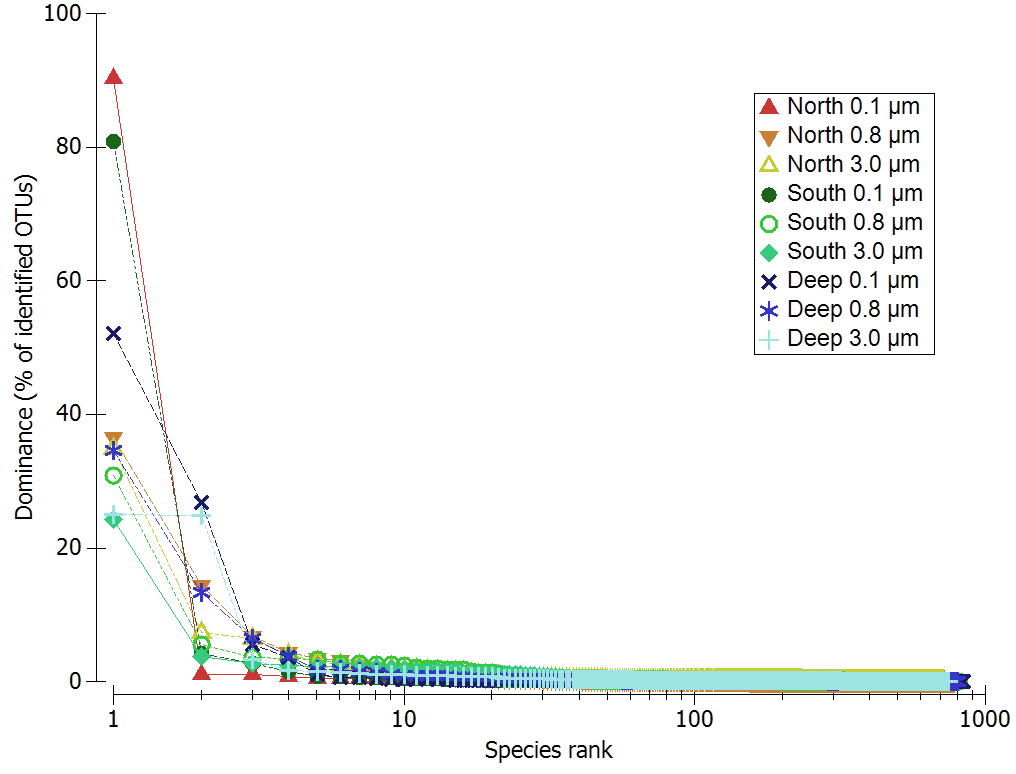
\includegraphics[width=\textwidth]{../polarfront/rankabundance.png}
  \caption[Rank-abundance curves for OTUs in each zone and size fraction]{Rank-abundance curves for OTUs identified in each zone and size fraction. The dominance of a given OTU is its relative abundance as a percentage of all identified OTUs. The x-axis is scaled logarithmically. Generated using \softwarename{PRIMER 6}.}
  \label{fig:rankabundance}
\end{figure}


\ac{ANOSIM} analysis showed that the zones harbor significantly different microbial communities (R = 0.45, p = 0.004). 
\ac{SIMPER} was performed in order to identify the contribution of individual \acp{OTU} to the difference between the \ac{NZ} and \ac{SZ}. 
The results for the highest contributors are provided in \tabreft{tab:otussimper}, and are graphically summarised for all \acp{OTU} in \figreft{fig:taxotreemap}.

\begin{sidewaystable}
\sffamily
\begin{center}
\caption[Highest-contributing \acp{OTU} to the difference between the North and South zones]{\sffamily{}
The thirty \acp{OTU} with the highest contributions to the difference between the \ac{NZ} and \ac{SZ}. 
  Abundances are zonal averages and have been standardised and log-transformed.
  As each \ac{OTU} on each size fraction was encoded as a separate variable in the \ac{SIMPER} analysis, the size fraction is given after each \ac{OTU} name.
  }
\label{tab:otussimper}
\begin{tabular}{llll}
\toprule
\textbf{OTU} & \textbf{Abundance} & \textbf{Abundance} & \textbf{Contribution to}\\
& \textbf{South} & \textbf{North} & \textbf{variance (\%)}\\

\midrule
\genus{Synechococcus} sp. CC9311 0.8 \micron & 0.00 & 1.08 & 2.88\\
\genus{Synechococcus} sp. CC9902 0.8 \micron & 0.00 & 1.04 & 2.81\\
\genus{Synechococcus} sp. CC9311 3.0 \micron & 0.01 & 0.98 & 2.59\\
\genus{Synechococcus} sp. CC9902 3.0 \micron & 0.04 & 0.76 & 2.03\\
\candidatusfull{Pelagibacter ubique} HTCC1062 3.0 \micron & 1.97 & 2.40 & 1.97\\
\candidatusfull{Ruthia magnifica} str. Cm (\speciesfull{Calyptogena magnifica}) 0.1 \micron & 0.82 & 0.25 & 1.57\\
\genus{Colwellia} sp. 34H 3.0 \micron & 0.34 & 0.66 & 1.32\\
\candidatusfull{Ruthia magnifica} str. Cm (\speciesfull{Calyptogena magnifica}) 0.8 \micron & 0.74 & 0.25 & 1.32\\
\candidatusfull{Pelagibacter ubique} HTCC1062 0.8 \micron & 2.32 & 2.48 & 1.32\\
\candidatusfull{Vesicomyosocius okutanii} strain HA 0.1 \micron & 0.62 & 0.18 & 1.20\\
\speciesfull{Coraliomargarita akajimensis} strain DSM 45221 0.8 \micron & 0.48 & 0.04 & 1.13\\
\speciesfull{Coraliomargarita akajimensis} strain DSM 45221 3.0 \micron & 0.49 & 0.06 & 1.10\\
\genus{Roseobacter} sp. OCh 114 0.8 \micron & 1.01 & 0.81 & 1.08\\
\speciesfull{Pseudoalteromonas atlantica} strain T6c 3.0 \micron & 0.38 & 0.54 & 1.08\\
\candidatusfull{Vesicomyosocius okutanii} strain HA 0.8 \micron & 0.57 & 0.19 & 1.04\\
\speciesfull{Acinetobacter baumannii} strain SDF 3.0 \micron & 0.45 & 0.18 & 0.95\\
\speciesfull{Gramella forsetii} strain KT0803 0.8 \micron & 0.72 & 0.43 & 0.94\\
\genus{Marinomonas} sp. MWYL1 0.8 \micron & 0.46 & 0.11 & 0.92\\
\genus{Roseobacter} sp. OCh 114 3.0 \micron & 0.76 & 0.54 & 0.91\\
\speciesfull{Flavobacterium psychrophilum} strain JIP02/86 0.8 \micron & 0.63 & 0.32 & 0.89\\
\speciesfull{Silicibacter pomeroyi} DSS-3 0.8 \micron & 0.75 & 0.69 & 0.86\\
\speciesfull{Brachyspira hyodysenteriae} strain WA1 3.0 \micron & 0.47 & 0.19 & 0.84\\
\candidatusfull{Ruthia magnifica} str. Cm (\speciesfull{Calyptogena magnifica}) 3.0 \micron & 0.34 & 0.21 & 0.82\\
\speciesfull{Pseudoalteromonas haloplanktis} strain TAC125 3.0 \micron & 0.22 & 0.33 & 0.77\\
\speciesfull{Robiginitalea biformata} strain HTCC2501 0.8 \micron & 0.61 & 0.40 & 0.74\\
\speciesfull{Nitrosopumilus maritimus} SCM1 0.1 \micron & 0.27 & 0.01 & 0.72\\
\speciesfull{Gramella forsetii} strain KT0803 3.0 \micron & 0.59 & 0.59 & 0.71\\
\speciesfull{Lysinibacillus sphaericus} strain C3-41 3.0 \micron & 0.29 & 0.02 & 0.71\\
\speciesfull{Nitrosopumilus maritimus} SCM1 0.8 \micron & 0.25 & 0.01 & 0.70\\
\speciesfull{Silicibacter} sp. TM1040 0.8 \micron & 0.59 & 0.55 & 0.69\\

\bottomrule
\end{tabular}
\end{center}
\end{sidewaystable}

\begin{figure}[!ht]
  \centering
  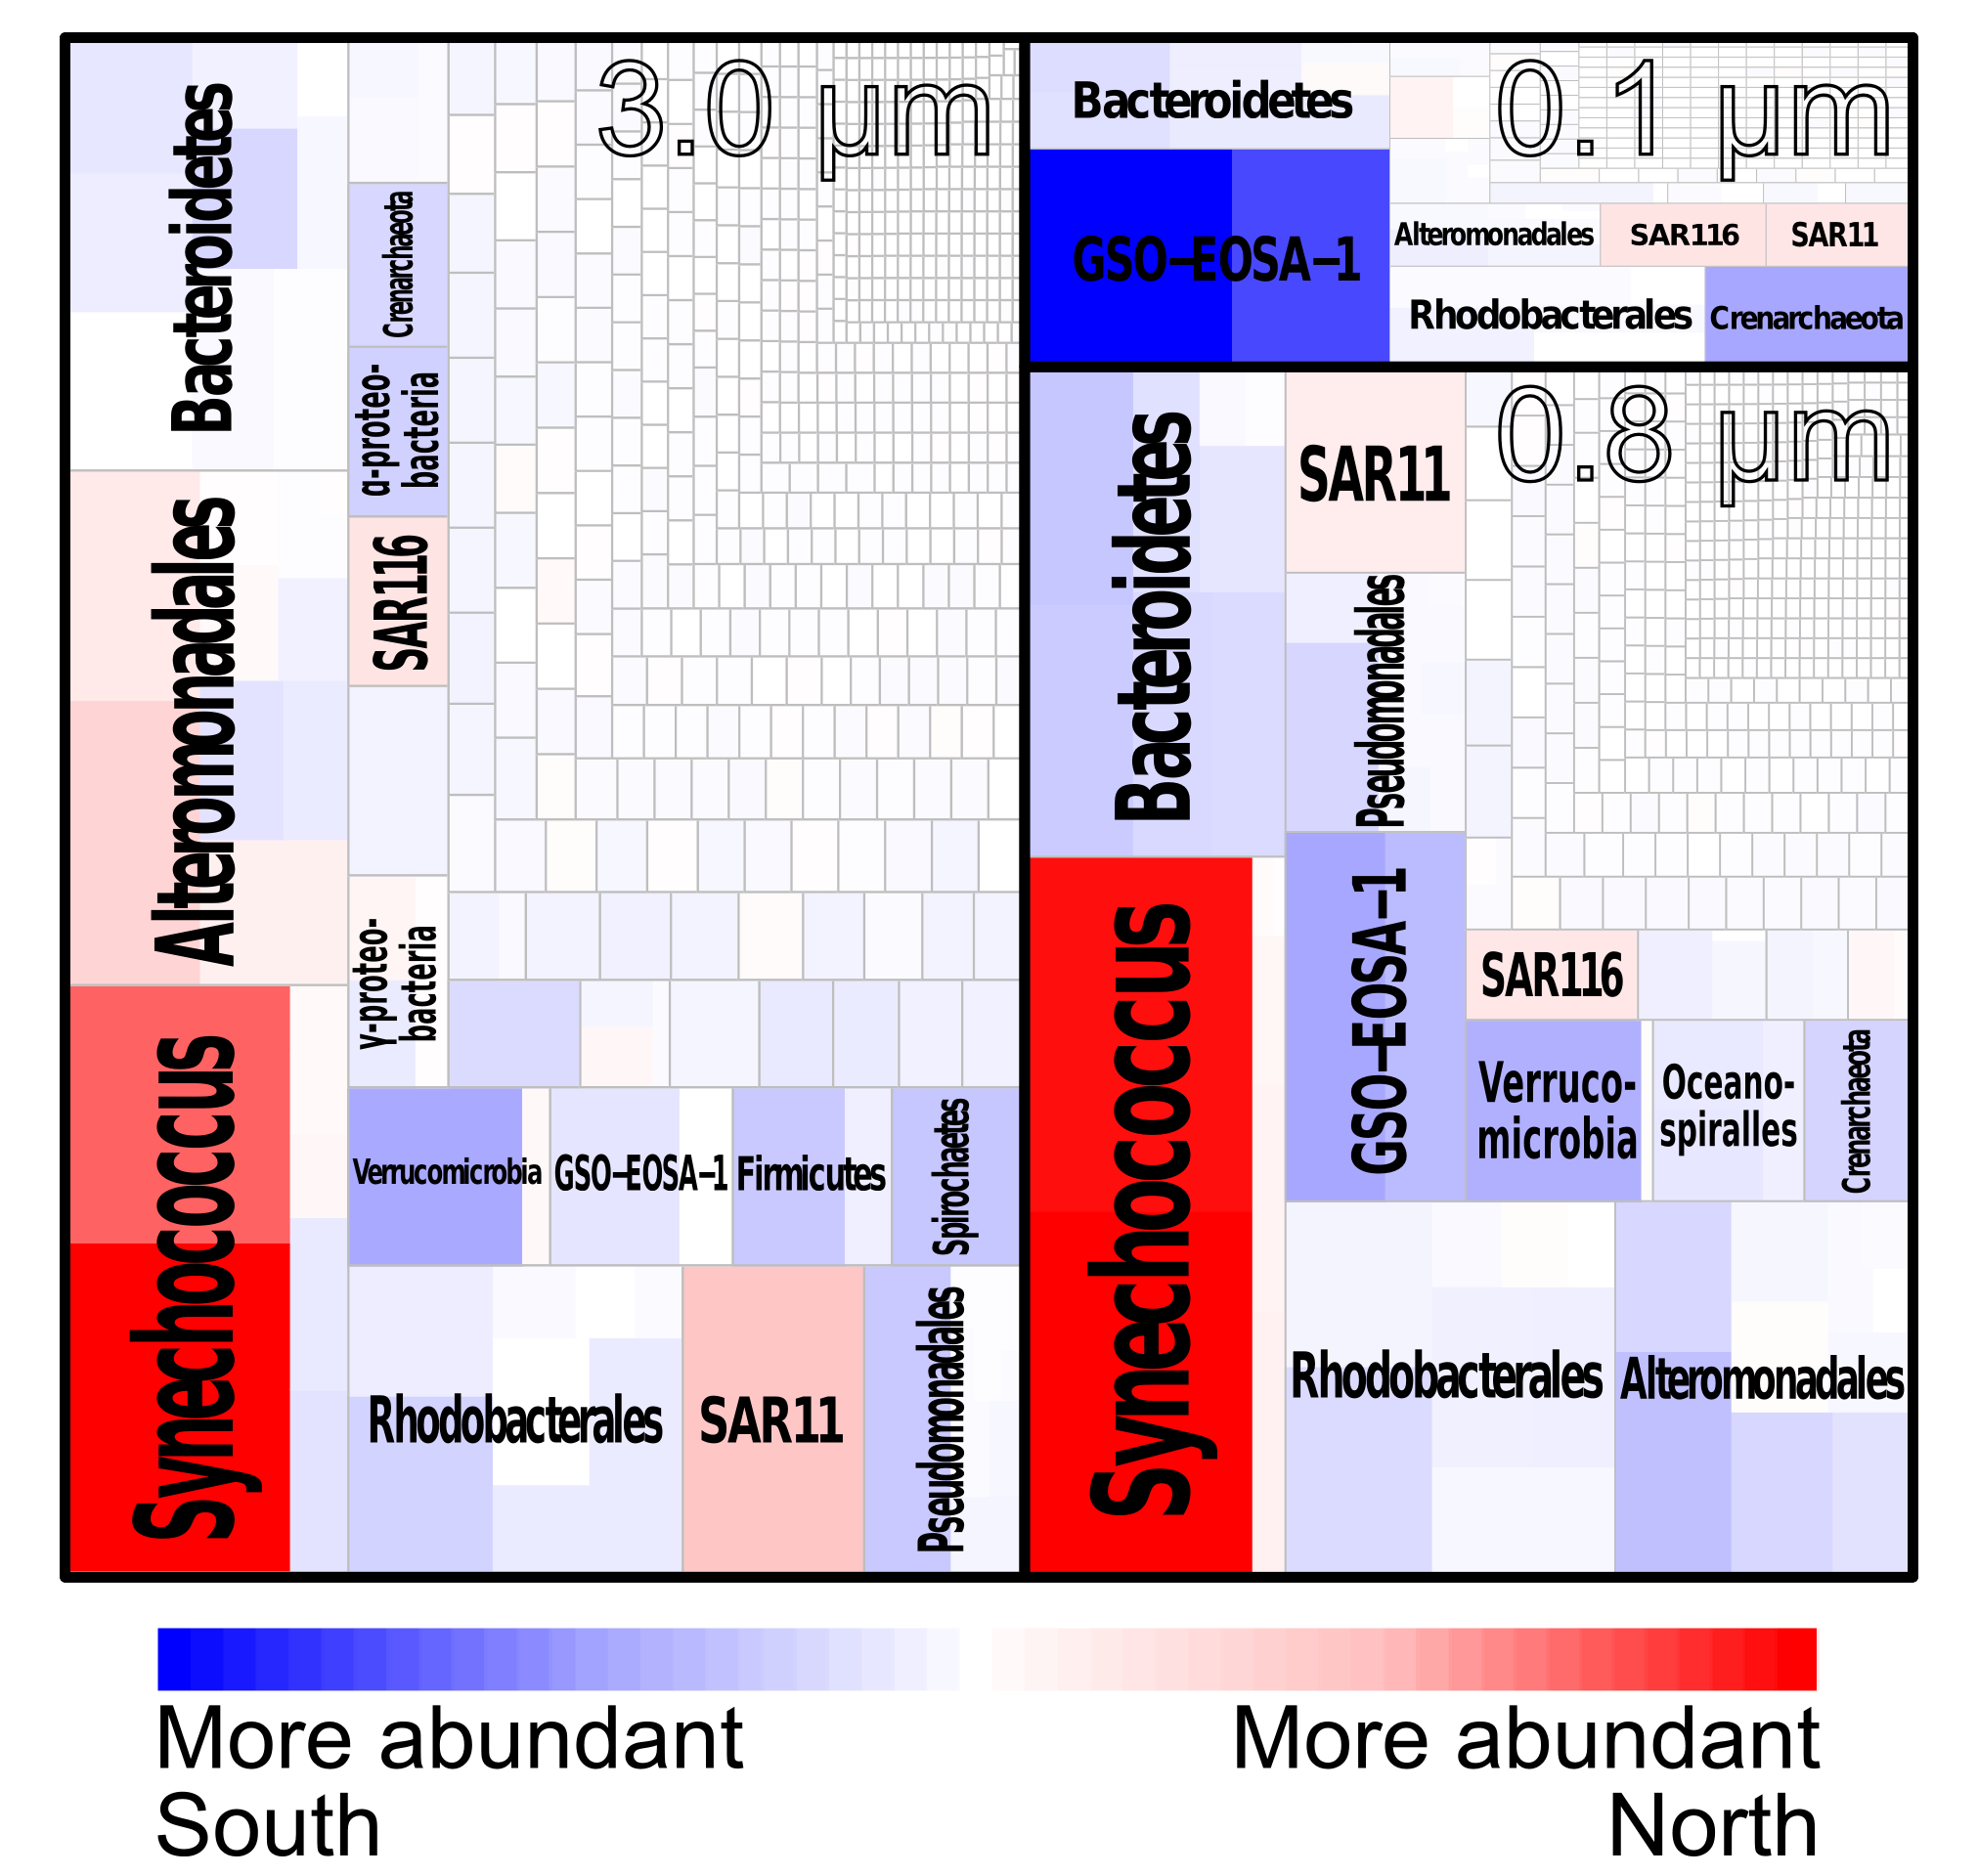
\includegraphics[width=\textwidth]{../polarfront/taxotreemap.png}
  \caption[Contribution of \acp{OTU} to variance between the North and South zones]{Contribution of \acp{OTU} to variance between the North and South zones, and differential abundance of \acp{OTU} from each size fraction between the two zones.
Each coloured (red or blue) rectangle represents an OTU identified through analysis of BLAST matches between SO metagenome data and the RefSeq database.
The area of each rectangle as a proportion of the total plot area corresponds to that \ac{OTU}'s contribution to the total variance between the two zones.
The colour of each rectangle corresponds to difference in relative abundance of that OTU between the zones, with blue indicating a higher relative abundance south of the PF, and red a higher abundance north of the PF.
\acp{OTU} from clades or taxonomic ranks of interest have been grouped, with labels in bold and groups separated by gray lines. 
Groups and \acp{OTU} with a low contribution to variance which were not grouped are unlabeled.
\acp{OTU} from each size fraction have also been grouped, with labels in black outline and size fractions separated by thick black lines. 
The data used to generate this figure are given in the supplementary material \suppfile{PF-OTUs-SIMPER.csv}.
  }
  \label{fig:taxotreemap}
\end{figure}


\ac{SIMPER} analysis found that no single \ac{OTU} contributed more than 2.9\% of variance, and 74\% of variance was contributed by \acp{OTU} with a contribution less than 1\%.
There was also a large difference in the contribution to variance of the three size fractions, with approximately 52\% of all variance contributed by \acp{OTU} from the 3.0 \micron{} fraction, 37\% by the 0.8 \micron{} fraction, and 9\% by the 0.1 \micron{} fraction.
Notably, \acp{OTU} within several taxonomic groups that had high contribution to variance covaried in their relative representation in the \ac{NZ} and \ac{SZ}.
For example, Bacteroidetes and GSO-EOSA-1 representatives were on average more abundant in the \ac{SZ}; while \genus{Prochlorococcus} and \genus{Synechococcus} species, SAR11 and SAR116 were on average more abundant in the \ac{NZ} \figref{fig:taxotreemap}.
Some groups, such as the Alteromonadales, had variable relative representation depending on size fraction.

\subsection{Fragment recruitment to verify \ac{OTU} identification}

As predicted, read recruitment to reference genomes produced fairly even coverage, especially in the high-abundance \acp{OTU}.
This indicates that \ac{OTU} identification was accurate and unlikely to be confounded by small regions of genomic identity.
\figreft{fig:frps} gives examples of read recruitment plots to three high-abundance and three low-abundance \acp{OTU}.

\afterpage{
  \centering
  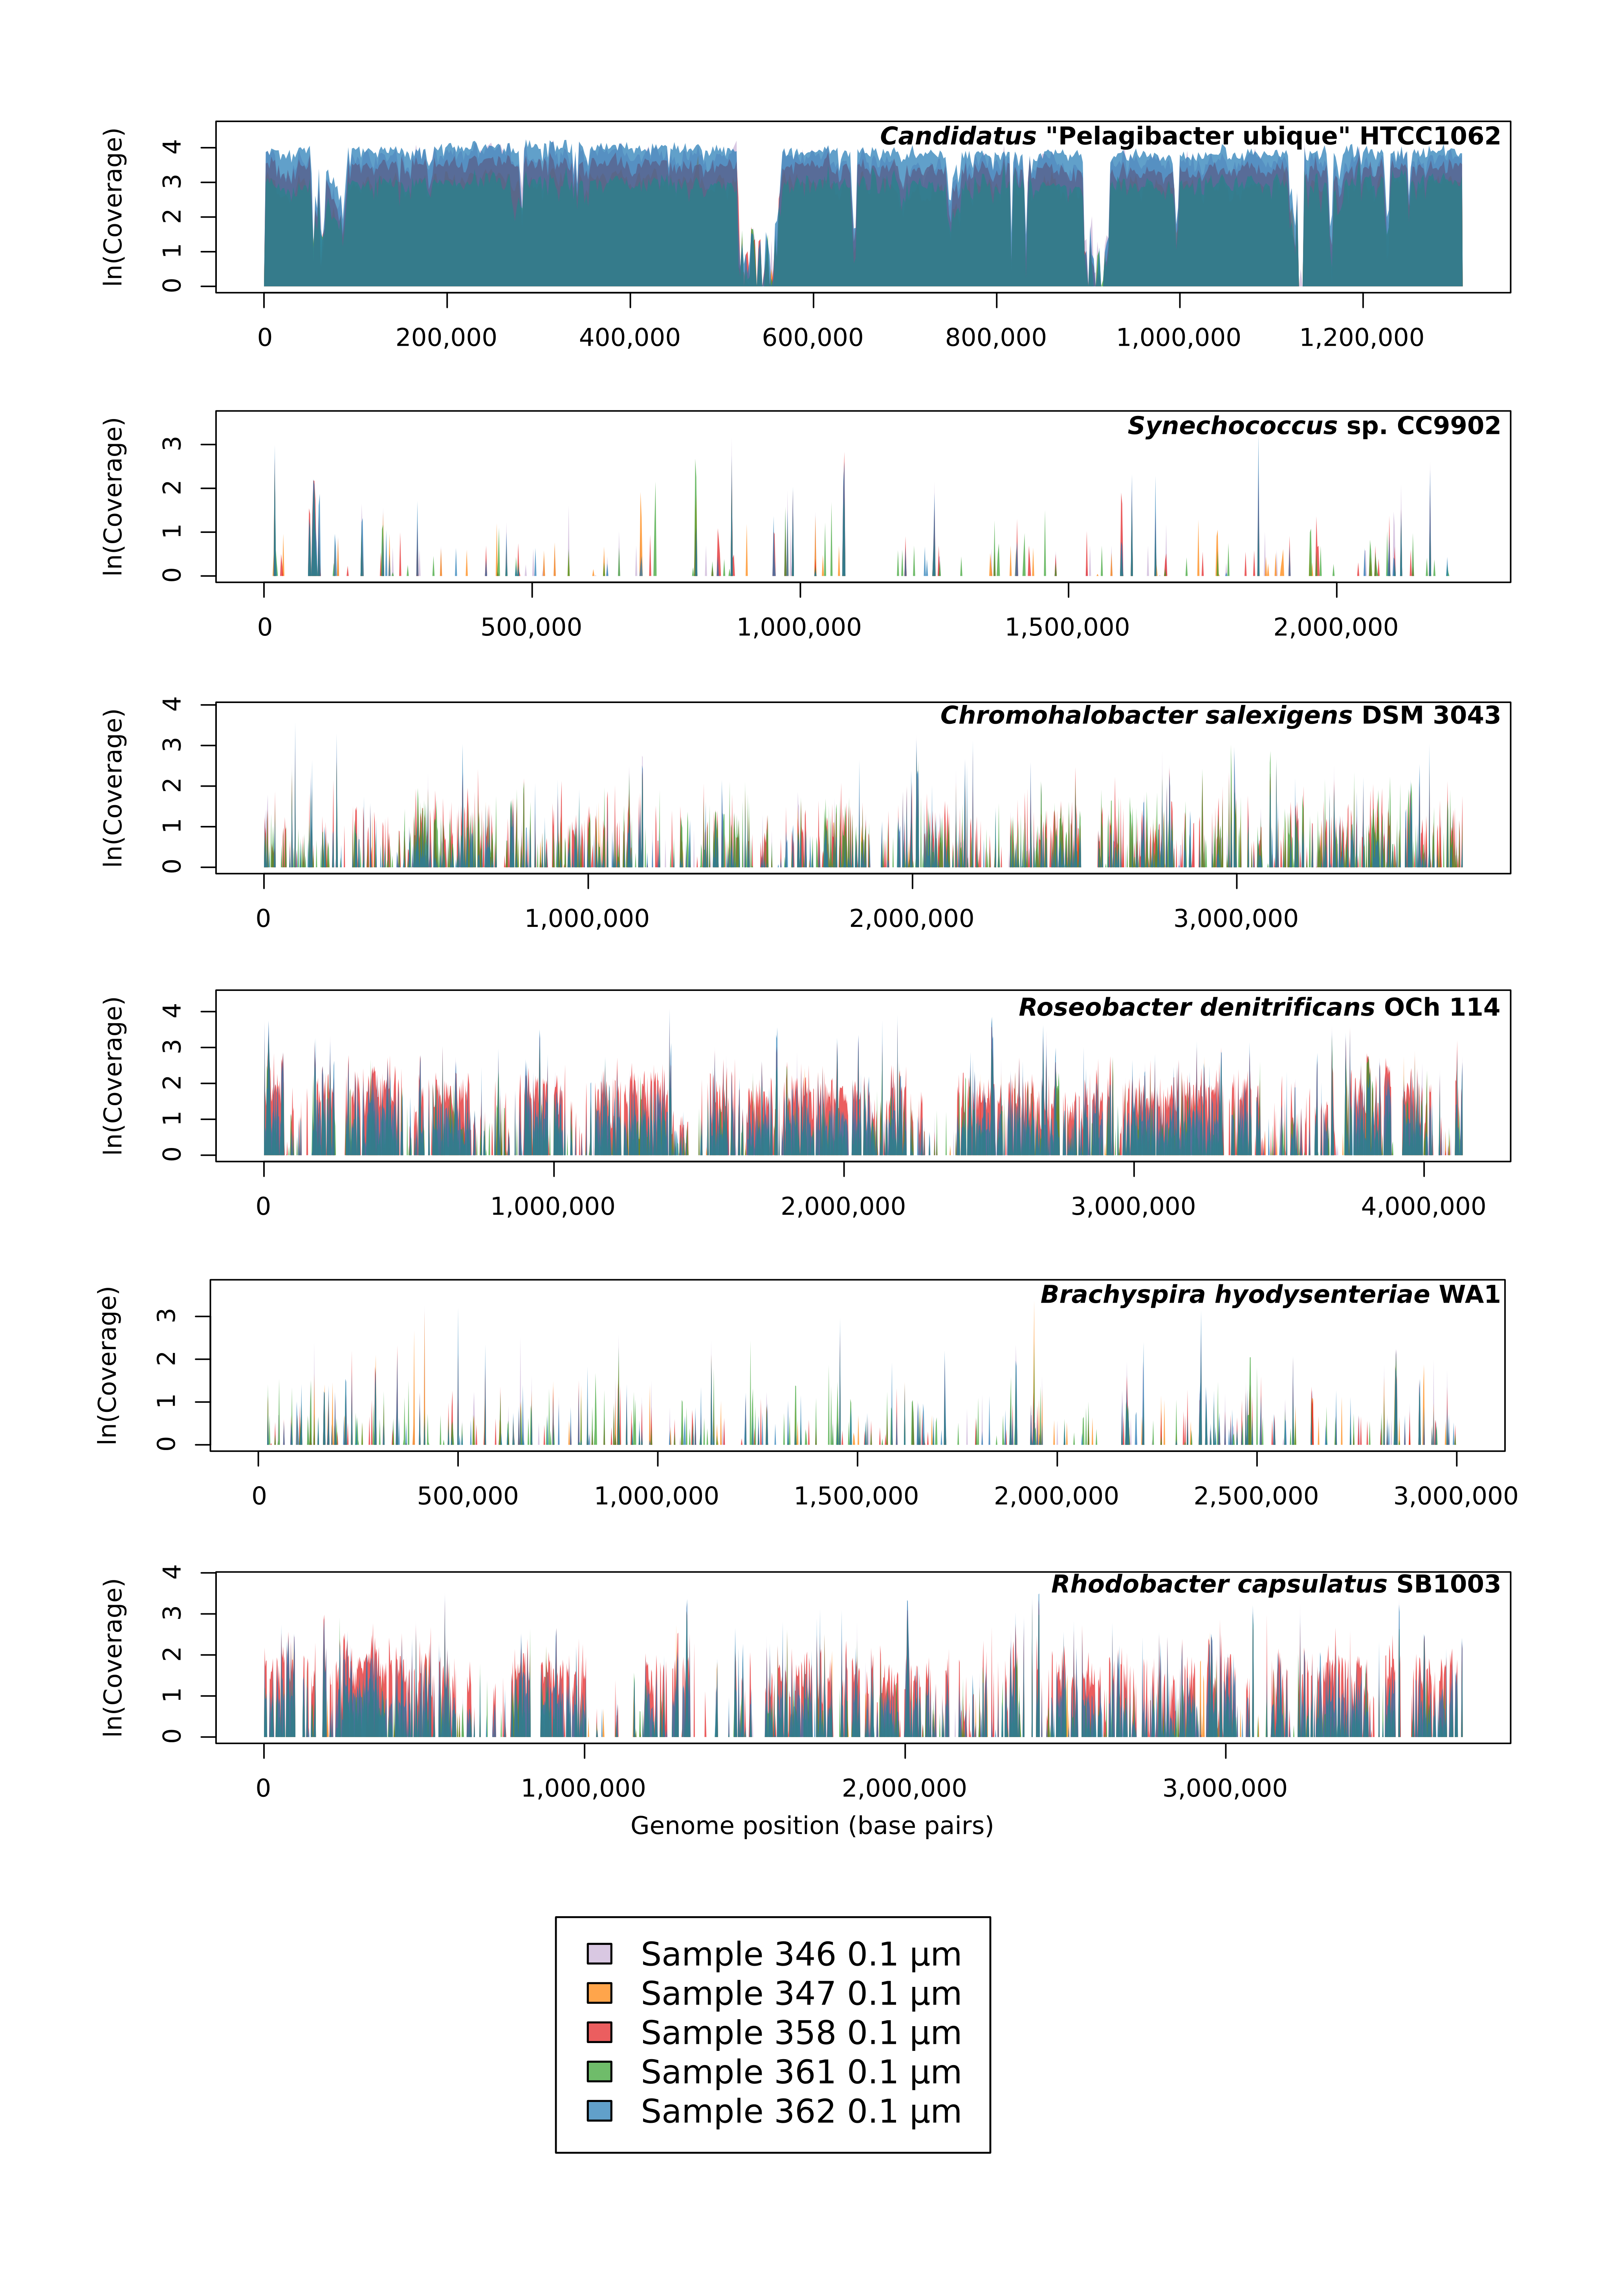
\includegraphics[height=\textheight]{../polarfront/frps.png}
  \captionof{figure}[Read recruitment to reference genomes]{\sffamily{}Examples of read recruitment (fragment recruitment) plots of metagenomic reads to reference genomes.
  The even distribution of recruitment sites across the genome suggests that \acp{OTU} identifications are relatively accurate; an \ac{OTU} identification resulting from a small region of genomic identity would generate a plot with read recruitment concentrated in small islands.
  \\
  \rule[1ex]{2cm}{0.5pt}
  }
  \label{fig:frps}
}


\subsection{Additional samples to test alternative ``polynya hypothesis''}
The \ac{ANOSIM} analysis strongly supported the ``\ac{PF} hypothesis'' (R = 0.44, p = 0.002), i.e.\ that the \ac{PF} was primarily responsible for the difference observed between the \ac{NZ} and \ac{SZ}, over the ``polynya hypothesis'' (R = 0.29, p = 0.005) that the influence of the Mertz Glacier polynya was responsible.
This also provides evidence that the \ac{PF} effect is robust over a longitudinal range and over time.

\subsection{Functional analysis of metagenomic data}

\ac{ANOSIM} analysis of the samples' \ac{KEGG} ortholog group and module profiles revealed that the zones had significantly different functional potential (ortholog group: R = 0.64, p = 0.001; module: R = 0.87, p = 0.001). 
\ac{SIMPER} was performed on the profiles in order to identify the specific functional differences between the zones. 
The highest-contributing modules are given in \tabreft{tab:modulessimper}, and a complete list in the supplementary material \suppfile{PF-modules-SIMPER.csv}.
The highest-contributing ortholog groups are given in \tabreft{tab:orthologsimper}, and a complete list in the supplementary material \suppfile{PF-ortholog-groups-SIMPER.csv}.
No single ortholog group or module contributed more than 2.2\% of the variance. 
There was a strong trend for ortholog groups and modules with higher contributions to variance to be overrepresented in the \ac{NZ} in the 3.0 \micron{} fraction but the \ac{SZ} in the smaller fractions, indicating that the functional diversity of each zone was strongly segregated by size fraction.

\begin{sidewaystable}
\sffamily
\begin{center}
\caption[Contributions of KEGG modules to variance between the North and South zones]{\sffamily{}The thirty \ac{KEGG} modules with the highest contributions to the difference between the \ac{NZ} and \ac{SZ}.
Abundances are zonal averages and have been standardised and log-transformed.
}
\label{tab:modulessimper}
\smallskip
\begin{tabularx}{\textwidth}{Xlll}
\toprule
\textbf{\ac{KEGG} module} & \textbf{Abundance} & \textbf{Abundance} & \textbf{Contribution to}\\
& \textbf{South} & \textbf{North} & \textbf{variance (\%)}\\
\midrule
Photosystem II & 0.42 & 0.57 & 2.21\\
Complex I (NADH dehydrogenase), NADH dehydrogenase I/diaphorase subunit of the bidirectional hydrogenase & 0.01 & 0.24 & 1.80\\
Photosystem I & 0.43 & 0.34 & 1.70\\
Pyrimidine deoxyribonucleotide biosynthesis, CDP/CTP \textrightarrow{} dCDP/dCTP,dTDP/dTTP & 0.51 & 0.66 & 1.16\\
Histidine degradation, histidine \textrightarrow{} N-formiminoglutamate \textrightarrow{} glutamate & 0.42 & 0.31 & 1.14\\
Methionine salvage pathway & 0.29 & 0.43 & 1.14\\
sn-Glycerol 3-phosphate transport system & 0.29 & 0.16 & 1.11\\
Complex I (NADH dehydrogenase), NADH dehydrogenase I & 1.08 & 1.05 & 1.06\\
Branched-chain amino acid transport system & 0.79 & 0.83 & 0.96\\
Dipeptide transport system & 0.14 & 0.02 & 0.95\\
Adenine nucleotide biosynthesis, IMP \textrightarrow{} ADP/dADP,ATP/dATP & 0.62 & 0.74 & 0.95\\
Glycine betaine/proline transport system & 0.66 & 0.56 & 0.94\\
Sulfur reduction, sulfate \textrightarrow{} H2S & 0.54 & 0.44 & 0.91\\
Simple sugar transport system & 0.46 & 0.39 & 0.90\\
Peptides/nickel transport system & 0.99 & 0.98 & 0.89\\
Ribosome, eukaryotes & 0.26 & 0.27 & 0.89\\
Multiple sugar transport system & 0.55 & 0.55 & 0.86\\
Type II general secretion system & 0.21 & 0.21 & 0.82\\
Sulfonate/nitrate/taurine transport system & 0.45 & 0.37 & 0.82\\
Guanine nucleotide biosynthesis, IMP \textrightarrow{} GDP/dGDP,GTP/dGTP & 0.72 & 0.82 & 0.81\\
RNA polymerase II, eukaryotes & 0.11 & 0.20 & 0.76\\
Histidine biosynthesis, PRPP \textrightarrow{} histidine & 0.94 & 0.86 & 0.76\\
Putrescine transport system & 0.18 & 0.09 & 0.72\\
Leucine biosynthesis, pyruvate \textrightarrow{} 2-oxoisovalerate \textrightarrow{} leucine & 1.29 & 1.37 & 0.71\\
C5 isoprenoid biosynthesis, non-mevalonate pathway & 0.70 & 0.77 & 0.71\\
Leucine degradation, leucine \textrightarrow{} acetoacetate + acetyl-CoA & 0.64 & 0.59 & 0.71\\
Thiamine transport system & 0.13 & 0.05 & 0.69\\
Spliceosome, 35S U5-snRNP & 0.18 & 0.20 & 0.68\\
Cytochrome b6f complex & 0.14 & 0.12 & 0.67\\
Menaquinone biosynthesis, chorismate \textrightarrow{} menaquinone & 0.25 & 0.27 & 0.66\\
\bottomrule
\end{tabularx}
\end{center}
\end{sidewaystable}

\begin{landscape}
\begin{table}
\sffamily
\begin{center}
\caption[Contributions of KEGG ortholog groups to variance between the North and South zones]{\sffamily{}
The thirty \ac{KEGG} ortholog groups with the highest contribution to the difference between the \ac{NZ} and \ac{SZ}.
Abundances are zonal averages and have been standardised and log-transformed.
As each ortholog group on each size fraction was encoded as a separate variable in the \ac{SIMPER} analysis, the size fraction is given after each ortholog group name.
}
\label{tab:orthologsimper}
\smallskip
\begin{tabularx}{\linewidth}{Xlll}
\toprule
\textbf{KEGG ortholog group} & \textbf{Abundance} & \textbf{Abundance} & \textbf{Contribution to}\\
& \textbf{South} & \textbf{North} & \textbf{variance (\%)}\\
\midrule
Hypothetical protein 3.0 \micron & 0.11 & 0.24 & 0.26\\
Hypothetical protein 0.8 \micron & 0.68 & 0.57 & 0.24\\
Ribonucleoside-diphosphate reductase alpha chain [EC:1.17.4.1] 0.8 \micron & 0.17 & 0.24 & 0.15\\
DNA polymerase III subunit alpha [EC:2.7.7.7] 0.8 \micron & 0.25 & 0.19 & 0.14\\
Hypothetical protein 0.1 \micron & 0.26 & 0.24 & 0.12\\
Proline dehydrogenase / delta 1-pyrroline-5-carboxylate 0.8 \micron & 0.10 & 0.04 & 0.12\\
Aminomethyltransferase [EC:2.1.2.10] 0.8 \micron & 0.25 & 0.19 & 0.12\\
Ribonucleoside-diphosphate reductase alpha chain [EC:1.17.4.1] 3.0 \micron & 0.02 & 0.08 & 0.12\\
Sarcosine oxidase, subunit alpha [EC:1.5.3.1] 0.8 \micron & 0.22 & 0.17 & 0.12\\
Integrator complex subunit 6 3.0 \micron & 0.07 & 0.05 & 0.11\\
Multicomponent Na$^{+}$:H$^{+}$ antiporter subunit D 0.8 \micron & 0.11 & 0.05 & 0.11\\
Glutamine synthetase [EC:6.3.1.2] 0.8 \micron & 0.24 & 0.19 & 0.11\\
Pyruvate dehydrogenase E1 component [EC:1.2.4.1] 0.8 \micron & 0.15 & 0.10 & 0.11\\
Cobaltochelatase CobN [EC:6.6.1.2] 0.8 \micron & 0.11 & 0.06 & 0.11\\
Formate dehydrogenase, alpha subunit [EC:1.2.1.2] 0.8 \micron & 0.15 & 0.10 & 0.11\\
DNA-directed RNA polymerase subunit beta [EC:2.7.7.6] 3.0 \micron & 0.03 & 0.08 & 0.11\\
Glutamate synthase (NADPH/NADH) large chain [EC:1.4.1.13 1.4.1.14] 0.8 \micron & 0.25 & 0.22 & 0.11\\
Dimethylglycine dehydrogenase [EC:1.5.99.2] 0.8 \micron & 0.17 & 0.14 & 0.11\\
Flagellin 0.8 \micron & 0.06 & 0.10 & 0.10\\
DNA-directed RNA polymerase subunit beta [EC:2.7.7.6] 3.0 \micron{}\footnote{Due to an error in the \ac{KEGG} database, this module is encoded twice.} & 0.03 & 0.08 & 0.10\\
Photosystem II PsbA protein 0.8 \micron & 0.01 & 0.06 & 0.09\\
Aldehyde dehydrogenase (NAD+) [EC:1.2.1.3] 0.8 \micron & 0.17 & 0.13 & 0.09\\
Glutamate synthase (NADPH/NADH) large chain [EC:1.4.1.13 1.4.1.14] 3.0 \micron & 0.02 & 0.07 & 0.09\\
Thymidylate synthase (FAD) [EC:2.1.1.148] 0.8 \micron & 0.02 & 0.06 & 0.09\\
Topoisomerase IV subunit A [EC:5.99.1.-] 0.8 \micron & 0.11 & 0.07 & 0.09\\
DNA mismatch repair protein MutS 0.8 \micron & 0.13 & 0.08 & 0.09\\
Glutamate dehydrogenase [EC:1.4.1.2] 0.8 \micron & 0.07 & 0.03 & 0.09\\
DNA polymerase I [EC:2.7.7.7] 0.1 \micron & 0.12 & 0.11 & 0.09\\
GTP-binding protein 0.8 \micron & 0.26 & 0.21 & 0.09\\
GTP-binding protein 3.0 \micron & 0.03 & 0.07 & 0.09\\
\bottomrule
\end{tabularx}
\end{center}
\end{table}
\end{landscape}


\section{Discussion}

\subsection{Taxonomic groups differentiating the zones}

\subsubsection{GSO-EOSA-1}

The Gammaproteobacterial Sulfur Oxidizer-EOSA-1 (GSO-EOSA-1) cluster, represented in RefSeq by the \acp{OTU} \candidatus{Vesicomyosocius okutanii} strain HA and \candidatus{Ruthia magnifica} strain Cm. (\species{Calyptogena magnifica}) \cite{Walsh:2009fja}, made a large contribution to variance between the \ac{NZ} and \ac{SZ}, with higher abundance in the \ac{SZ}: relative abundances of GSO-EOSA-1 in the \ac{SZ} were 5.2\%, 3.4\% and 0.25\% in the 0.1, 0.8 and 3.0 \micron{} size fractions respectively, compared to 1.1\%, 0.84\% and 0.30\% in the \ac{NZ} \tabref{tab:topotus}.
The contribution to variance of this group was highest in the 0.1 \micron{} size fraction, followed by 0.8 \micron{} and 3.0 \micron{} \tabref{tab:otussimper}.
This pattern most likely represents a small cell size and lack of association with particulate matter.

\candidatus{Ruthia magnifica} and \candidatus{Vesicomyosocius okutanii} are chemoautotrophic endosymbionts of deep-sea bivalves \cite{Kuwahara:2007gf,Newton:2007fu} and are thus unlikely to be present in open ocean surface waters. 
However, GSO-EOSA-1 representative ARCTIC96BD-19 has recently been reported at high abundance in Antarctic coastal waters \cite{Ghiglione:2011ee,Grzymski:2012ej}.
The majority of 16S rRNA genes from this metagenome with best \softwarename{blastn} hits to \candidatus{Ruthia magnifica} and \candidatus{Vesicomyosocius okutanii} clustered with ARTIC96BD-19 in a neighbour-joining phylogenetic tree \figref{fig:GSO-EOSA-1tree}, indicating this is the dominant GSO-EOSA-1 representative. 

\begin{figure}[!ht]
  \centering
  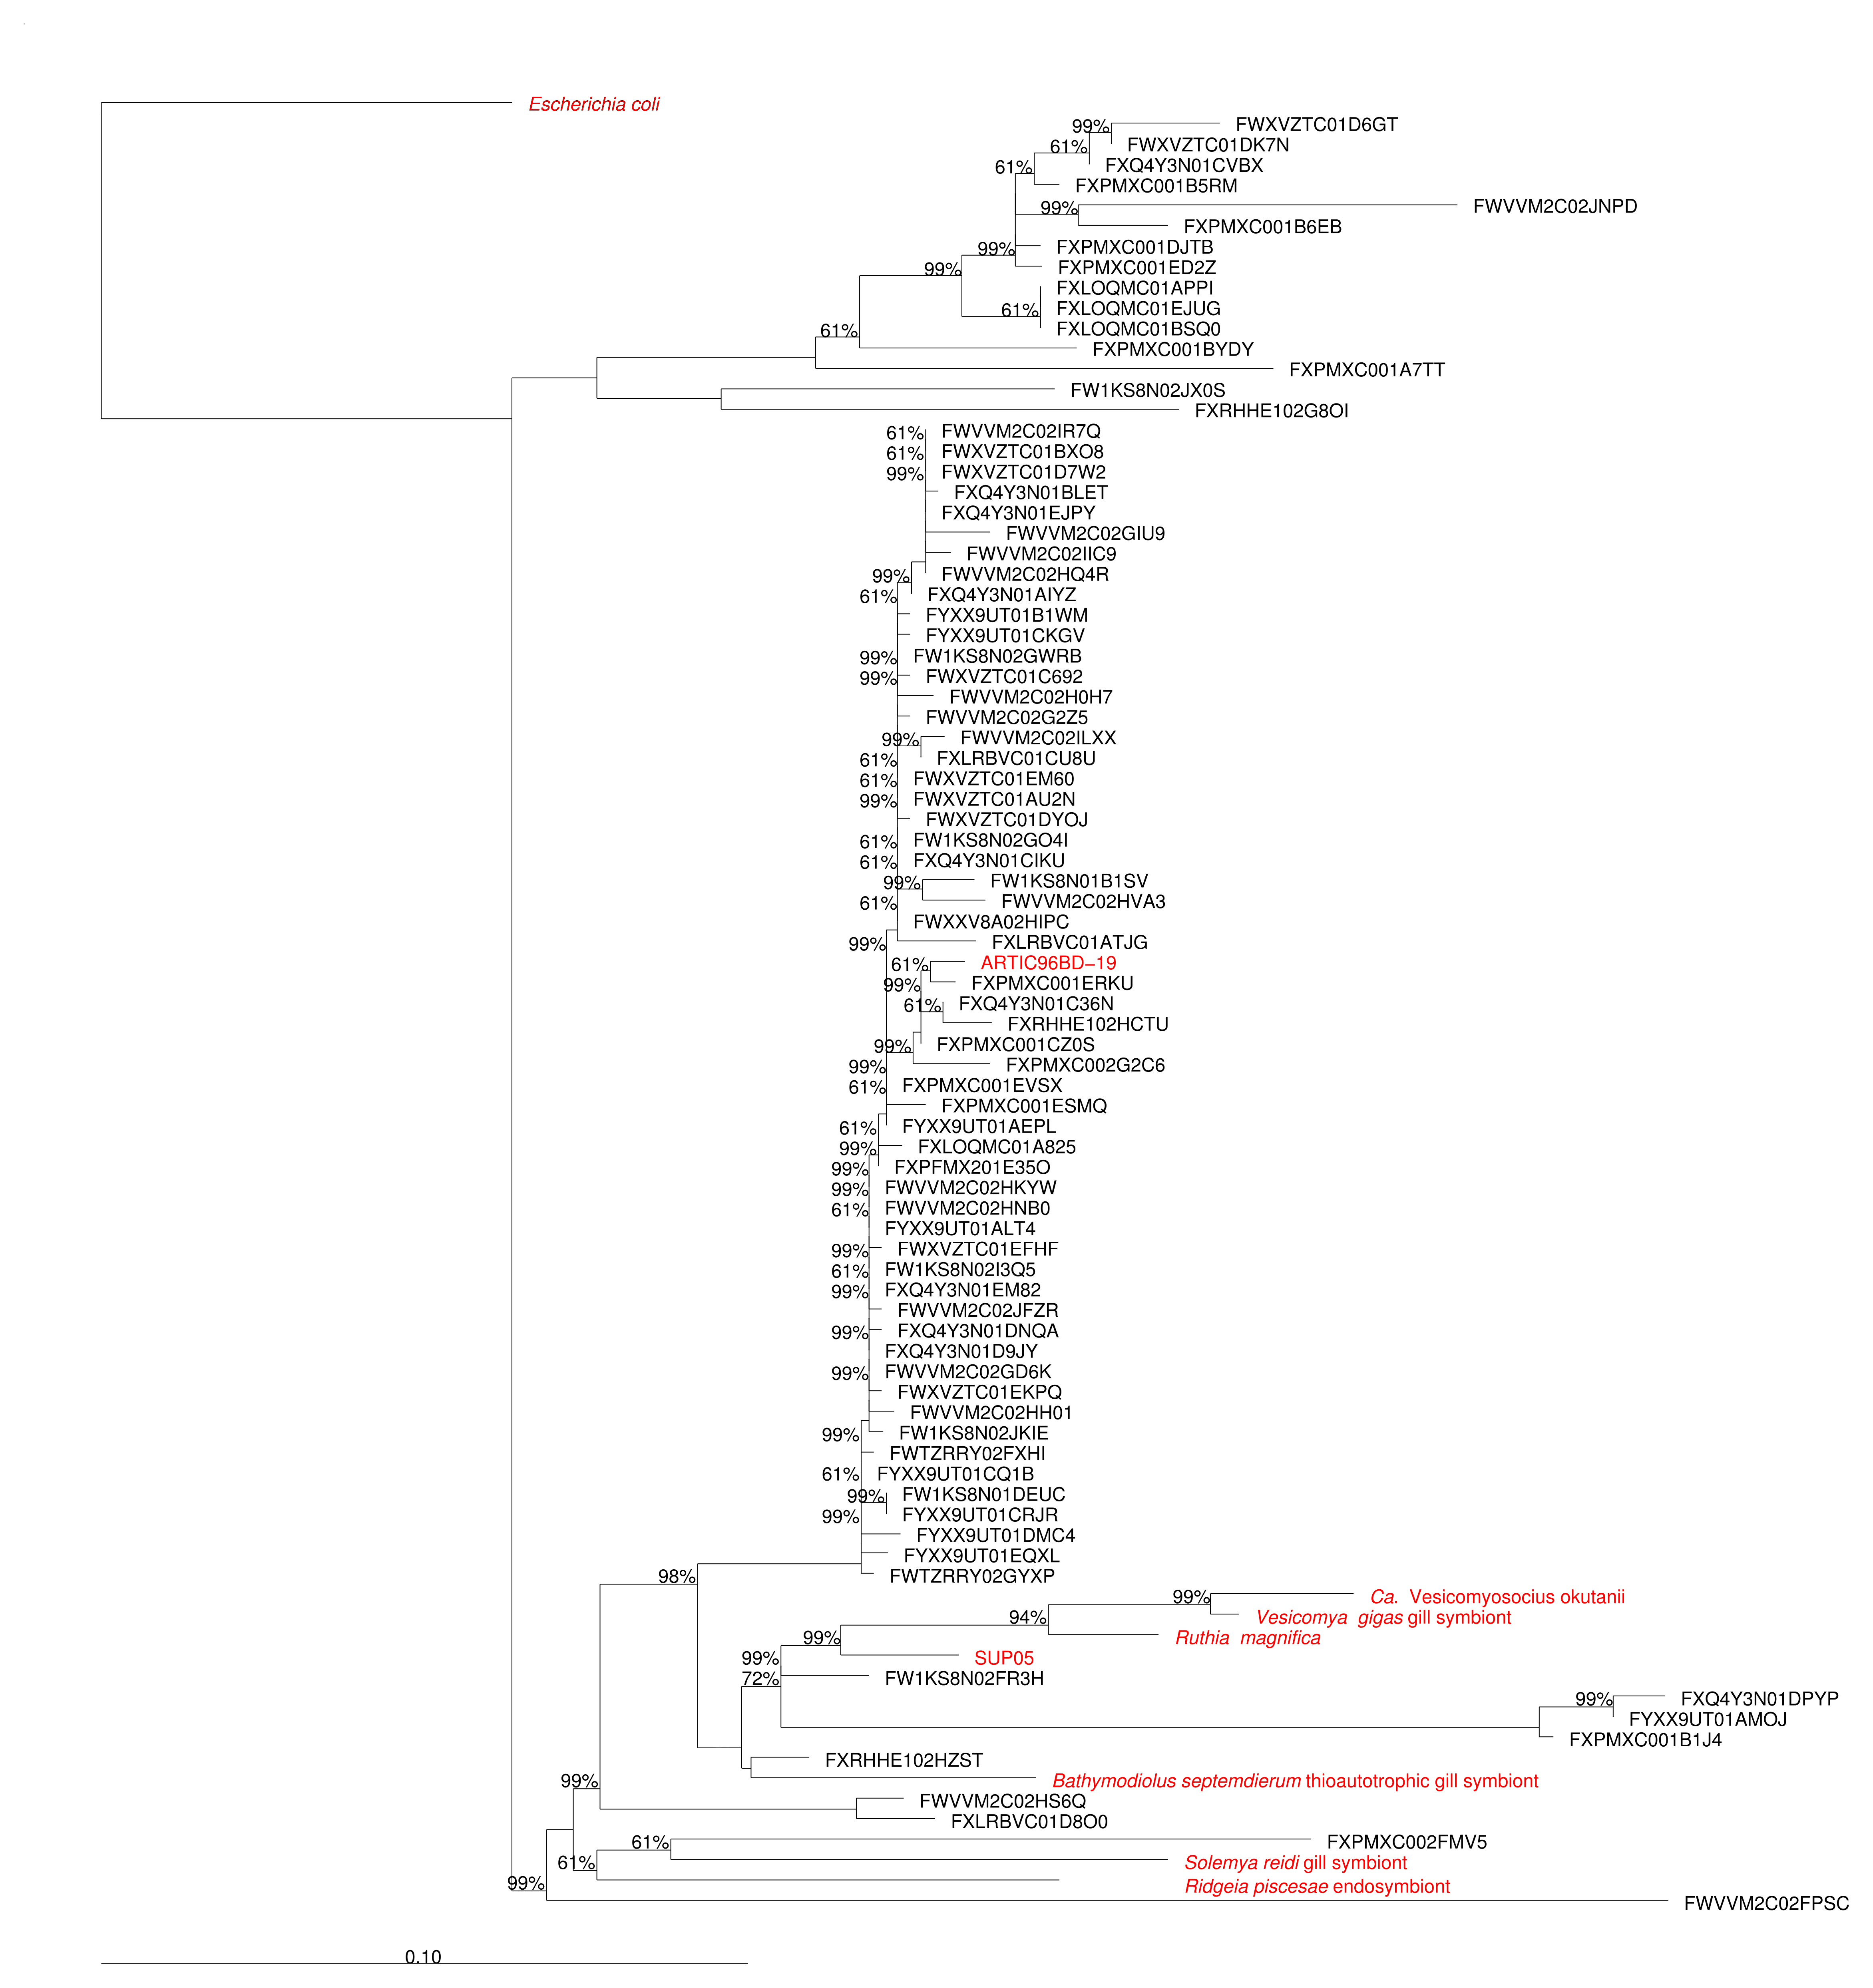
\includegraphics[width=\textwidth]{../polarfront/GSO-EOSA-1tree.png}
  \caption[Tree of GSO-EOSA-1 related 16S rRNA genes]{
  Neighbour-joining tree of GSO-EOSA-1-like 16S rRNA gene sequences from the metagenomes in this study.
  Sequences labeled in black text are reads from the metagenomes.
  Red labels are 16S rRNA gene sequences from Gammaproteobacterial Sulfur Oxidizers (GSO) and other Gammaproteobacteria.
  Bootstrap values for each node are indicated as percentages.
  The tree was constructed using \softwarename{arb} \cite{Ludwig:2004dg}.
  }
  \label{fig:GSO-EOSA-1tree}
\end{figure}
\clearpage

Single-cell genomic analysis of ARCTIC96BD-19 from global mesopelagic waters indicates the lineage is probably mixotrophic, able to couple carbon fixation to oxidation of reduced sulphur compounds as well as assimilate organic carbon \cite{Swan:2011hb}.
GSO-EOSA-1 cytochrome C oxidase (CoxII) has been identified in a winter metaproteome of Antarctic Peninsula coastal waters, suggesting the capacity for aerobic respiration \cite{Williams:2012bs}.
Taken together, this evidence suggests the GSO-EOSA-1 representative in Antarctic coastal waters is a versatile chemolithoautotroph capable of aerobic respiration.

It has been proposed that during the winter months, chemolithoautotrophy is dominant over photoautotrophy as the major carbon fixation process in \ac{AZ} waters due to the lack of available light, both from seasonal darkness and ice shading \cite{Grzymski:2012ej}.
The high relative abundance of GSO-EOSA-1 in \ac{SZ} compared to \ac{NZ} waters may therefore represent the remnants of an annual winter increase in population in the marginal ice zone which does not occur in the open ocean.

\subsubsection{Ammonia-oxidizing Crenarchaeota}

\species{Nitrosopumilus maritimus} SCM1 and \species{Cenarchaeum symbiosum} are chemolithoautotrophic, nitrifying members of the \ac{MGI} \cite{Preston:1996vi,Walker:2010ww} and are the only representatives in the reference database of the \ac{AOA}.
The contribution of \acp{OTU} of \species{Cenarchaeum symbiosum} to the \ac{AOA} signature was low.
As \species{Cenarchaeum symbiosum} is a sponge symbiont \cite{Preston:1996vi} and given the poor representation of \ac{AOA} in RefSeq, it is likely this \ac{OTU} has attracted sequences originating from planktonic \ac{AOA} and \species{Cenarchaeum symbiosum} itself is not present.
\ac{AOA} were moderate contributors to variance between the \ac{NZ} and \ac{SZ}, and were overrepresented in the \ac{SZ} in all size fractions \figref{fig:taxotreemap}.
As with the GSO-EOSA-1 cluster, \ac{MGI} have been proposed to be abundant chemolithoautotrophs and therefore major drivers of winter carbon fixation in Antarctic coastal waters \cite{Grzymski:2012ej,Williams:2012bs}.

Sample 353 had a particularly high relative abundance of \species{Nitrosopumilus maritimus} \acp{OTU} (7.5\% of the 0.1 \micron{} fraction; 0.8 \micron: 11\%; 3.0 \micron: 12\%).
This sample was taken closer to the Antarctic continent (3.7 km) than any other, in relatively shallow (180 m) waters 17.6 km from the Mertz Glacier.
The high abundance of ammonia oxidizers may reflect an input of ammonia from terrestrial sources (e.g.\ penguin guano), or resuspension of benthic sediments in which \ac{MGI} are abundant \cite{Bowman:2003fa} by near-shore turbulence and iceberg scouring.
Breakdown of water column stratification has been previously suggested as a cause of increased \ac{AOA} abundance in Antarctic coastal surface waters \cite{Kalanetra:2009bv}.

\subsubsection{Cyanobacteria}

\acp{OTU} of the cyanobacterial genera \genus{Prochlorococcus} and \genus{Synechococcus} were overrepresented in the \ac{NZ} in all size fractions \figref{fig:taxotreemap}.
The mean relative abundance of cyanobacteria in samples 367 and 368, the two northernmost samples, was strikingly higher than the mean abundance across all other samples in the \ac{NZ}.
\genus{Synechococcus} sp. CC9902 alone composed greater than 22\% of the 0.8 \micron{} fraction in these samples, consistent with \genus{Synechococcus} species' average cell diameter of approximately 0.9 \micron.
The high abundance of both cyanobacterial genera on the 3.0 \micron{} fraction has previously been reported \cite{Lauro:2010jna} and may be attributable to aggregation \cite{Lomas:2011bp}.

Samples 367 and 368 were separated from the other samples north of the \ac{PF} by the \ac{STF}.
While the \ac{STF} was not a significant boundary on the assemblage level, it may mark a significant biogeographic boundary for these cyanobacteria.
\genus{Synechococcus} and \genus{Prochlorococcus} together represent a large proportion of both phytoplankton abundance and carbon fixation in temperate and tropical waters, in many regions contributing more than half of total primary production \cite{Liu:1997ub,Liu:1998tk,Andre:1999uh}.
The role of the \ac{STF} in determining the latitudinal range of \genus{Synechococcus} and \genus{Prochlorococcus} is therefore important, as it will affect models of ocean productivity under changing climactic conditions, and warrants further investigation.
Despite the high abundance of cyanobacteria north of the \ac{STF}, they were also a significant feature of the \ac{SAZ}; for example, \genus{Synechococcus} sp. CC9902 composed 3--5\% of the 0.8 \micron{} fraction in \ac{SAZ} samples.

These results extend the latitudinal distribution of both \genus{Prochlorococcus} and \genus{Synechococcus} to include presence at very low abundance as far south as the Antarctic coast.
\genus{Prochlorococcus} have been reported to be restricted to tropical and subtropical waters within 40\textdegree{} of latitude \cite{Partensky:1999uf}, and to be a negligible \cite{Ghiglione:2011ee} or undetectable \cite{Grzymski:2012ej} component of marine microorganisms in Antarctic waters.
However, these findings are consistent with findings of a logarithmic relationship of cyanobacterial numbers with temperature, where cyanobacteria were found at concentrations of 103--104 cells per litre even in the coldest waters, approximately four orders of magnitude less than in waters around Tasmania \cite{Marchant:1987wv}.
Cyanophage proteins have also been detected in a metaproteomic analysis of Antarctic Peninsula coastal surface waters \cite{Williams:2012bs}.

\subsubsection{SAR11 and SAR116 clades}

\candidatus{Pelagibacter ubique} HTCC1062 is a good representative of total SAR11 abundance in this study, as it is a member of the SAR11 phylotype which is most abundant in \ac{SO} waters \cite{Brown:2012gna}.
\candidatus{Pelagibacter ubique} HTCC1062 was the most abundant \ac{OTU} across all samples and fractions (\ac{NZ} average: 62\%, 25\% and 24\% of the 0.1 \micron{}, 0.8 \micron{} and 3.0 \micron{} fractions respectively; \ac{SZ}: 59\%, 22\% and 18\%) and one of the most significant contributors to variance between the \ac{NZ} and \ac{SZ}.
The high abundance of SAR11 in the 0.1 \micron{} fraction is consistent with the small size of SAR11 cells \cite{Rappe:2002wz}.
The higher representation in the \ac{NZ} may reflect the competitiveness of SAR11 members in regions with low \ac{DOC} concentrations due to low primary productivity \cite{Giovannoni:2005ib,Alonso:2006dj}, such as the \ac{HNLC} \ac{SAZ}.
Overall, these findings are consistent with reports that SAR11 is ubiquitous in the world's oceans \cite{Mary:2006wk,Carlson:2009cc} and more abundant north of the \ac{ACC} \cite{Giebel:2009hr}.

\acp{OTU} of \candidatus{Puniceispirillum marinum} from the SAR116 clade were a moderate contributor to variance between the \ac{NZ} and \ac{SZ} with higher abundance in the \ac{NZ} \figref{fig:taxotreemap}.
A genomic analysis reported \candidatus{Puniceispirillum marinum} IMCC1322 to be a metabolic generalist with genes for aerobic CO fixation, C1 metabolism and a \candidatus{Pelagibacter ubique}-like \ac{DMSP} demethylase, suggesting SAR116 and SAR11 occupy similar ecological niches \cite{Oh:2010di}.
In the Scotia Sea, SAR116 abundance (determined using \ac{FISH}) was reported to be higher in more productive waters where SAR11 numbers were lower \cite{Topping:2006ul}.
However, this analysis across an extended latitudinal transect indicates that overall SAR11 and SAR116 have similar biogeographic distributions.

\subsubsection{Bacteroidetes}

\acp{OTU} of the phylum Bacteroidetes, in particular members of the class Flavobacteria, were found to be abundant (\ac{NZ} average: 1.2\%, 5.0\% and 6.9\% of the 0.1 \micron{}, 0.8 \micron{} and 3.0 \micron{} fractions respectively; SZ: 2.3\%, 9.8\% and 9.1\%) and significant contributors to variance between the \ac{NZ} and \ac{SZ} \figref{fig:taxotreemap}.
Flavobacteria have been previously reported to compose the majority of both Bacteroidetes \cite{Murray:2007db} and total planktonic biomass \cite{Abell:2005ji} in the \ac{SO}, as well as being abundant in sea ice \cite{Brown:2001hh}.
As heterotrophic degraders of \ac{HMW} compounds in the form of both \ac{DOM} and \ac{POM} \cite{Kirchman:2002ub}, marine Flavobacteria are major components of marine aggregates \cite{Rath:1998wm,Crump:1999wo,Zhang:2007fb}.
The higher abundance of Flavobacteria \acp{OTU} on the 0.8 \micron{} and 3.0 \micron{} fractions indicates their association with particulate matter.
Similar size partitioning of \ac{SO} Flavobacteria has previously been reported \cite{Abell:2005ji}.

The higher abundance of \acp{OTU} of Flavobacteria in the \ac{SZ} may reflect an input of cells from melting sea ice \cite{Brown:2001hh}, the higher rates of primary productivity in the south, and the role of the Flavobacteria as degraders of \ac{HMW} \ac{DOM}.
Because deposition of marine snow is a major route for sequestration of fixed carbon in the ocean \citep[e.g.][]{Hessen:2004vq}, the Flavobacteria that associate with this particulate matter represent a remineralising shunt, which would decrease carbon sequestration by this route.

\subsubsection{Rhodobacterales}

Members of the order Rhodobacterales were abundant (\ac{NZ} average: 1.2\%, 10\% and 5.5\% of the 0.1 \micron{}, 0.8 \micron{} and 3.0 \micron{} fractions respectively; \ac{SZ}: 1.6\%, 13\% and 7.9\%) and high contributors to variance, overrepresented in the \ac{SZ} on all size fractions.
As several members of the Roseobacter clade have been shown to have symbiotic relationships with marine eukaryotic algae \cite{Buchan:2005hd,WagnerDobler:2006kb}, and their abundance in the \ac{SO} has previously been linked to phytoplankton blooms \cite{West:2008kc,Obernosterer:2011df}, it is likely that their overrepresentation in the \ac{SZ} is related to the higher density of phytoplankton in the \ac{AZ}.

\acp{OTU} of \species{Roseobacter denitrificans} Och114 and \species{Silicibacter pomeroyi} DSS-3 were consistently the most abundant Roseobacter clade representatives.
\species{Roseobacter denitrificans} and \species{Silicibacter pomeroyi} fall within a subclade of \ac{AAP} members of the Roseobacter clade \cite{Swingley:2007dm}.
These species have diverse mixotrophic metabolisms, with genomic and experimental evidence of photoheterotrophic respiration of organic carbon, fixation of \ce{CO_{2}}, oxidation of CO, oxidation of reduced sulfur compounds, and utilization of the abundant marine osmolyte \ac{DMSP} \cite{King:2003kc,Moran:2004ie,WagnerDobler:2006kb,Swingley:2007dm,Brinkhoff:2008do,Howard:2008hf}.
This metabolic diversity suggests a complex ecological role, particularly with respect to the capture and release of climatically active gases (\ce{CO_{2}}, CO, dimethylsulfide) involved in carbon and sulfur cycling.

\subsubsection{Alteromonadales}

Members of the gammaproteobacterial order Alteromonadales were large contributors to variance.
Most \acp{OTU} were overrepresented in the \ac{SZ} but some were overrepresented in the \ac{NZ} on the 3.0 \micron{} fraction \figref{fig:taxotreemap}.
\species{Colwellia psychrerythraea} 34H was one of the most abundant \acp{OTU} in the Alteromonadales that exhibited this distribution (\ac{NZ} average: 0.14\%, 2.2\% and 16\% of the 0.1 \micron{}, 0.8 \micron{} and 3.0 \micron{} fractions respectively; \ac{SZ}: 0.52\%, 5.1\% and 10\%).
\species{Colwellia psychrerythraea} 34H was isolated from Arctic sediment, grows well at low temperatures and secretes extracellular polysaccharides \cite{Huston:2000jr,Junge:2003kb,Methe:2005uf}.
Similar to other \genus{Colwellia} species grown under laboratory conditions, cells have widths of 0.4--0.8 \micron{} and lengths of 1.5--4.5 \micron{} \cite{Jung:2006fh}.
Growth temperature can have a major impact on cell morphology, enzyme secretion and global gene expression in psychrophiles \citep[e.g.][]{Feller:2003ir,Junge:2003kb,Williams:2011hy,Cavicchioli:2006bl,Campanaro:2011gj}.
Moreover, marine bacteria can alter their cell dimensions in response to nutrient flux \citep[e.g.][]{Kjelleberg:1987wp}.
It is therefore possible that the populations of Alteromonadales captured on the 3.0 \micron{} filters (overrepresented in the \ac{NZ}) had different physiological properties to those on the 0.1 and 0.8 \micron{} filters (overrepresented in the \ac{SZ}).

\subsubsection{Verrucomicrobia}

Two representatives of the phylum Verrucomicrobia, \species{Coraliomargarita akajimensis} and \genus{Akkermansia} sp. Muc-30, were moderate contributors to variance and overrepresented in the \ac{SZ} \figref{fig:taxotreemap}.
Surprisingly given the small cell size of \species{Coraliomargarita akajimensis} \cite{Yoon:2007ic}, its contribution to variance increased with size fraction.
A global survey reported a similar fractionation pattern, and suggested marine Verrucomicrobia may be predominantly particle attached \cite{Freitas:2012jz}.
However, little else is known about the distribution and ecological roles of marine Verrucomicrobia \cite{Freitas:2012jz}.

\subsection{Functional capacities differentiating the zones}

A number of modules with transport functions (sn-glycerol 3-phosphate transport system, dipeptide transport system, peptides/nickel transport system, simple sugar transport system, sulfonate/nitrate/taurine transport system) were overrepresented in the \ac{SZ} \tabref{tab:modulessimper}.
As the genomes of copiotrophic bacteria have evolved to have a higher number of narrow-specificity transporters relative to oligotrophic genomes \cite{Lauro:2009gx}, these differences may reflect the higher nutrient availability and thus a dominance of copiotrophs in the \ac{SZ}.
The taxonomic contributors to these modules were varied, although members of the Rhodobacterales were prominent \figref{fig:moduledecomp}.

\afterpage{
  \centering
  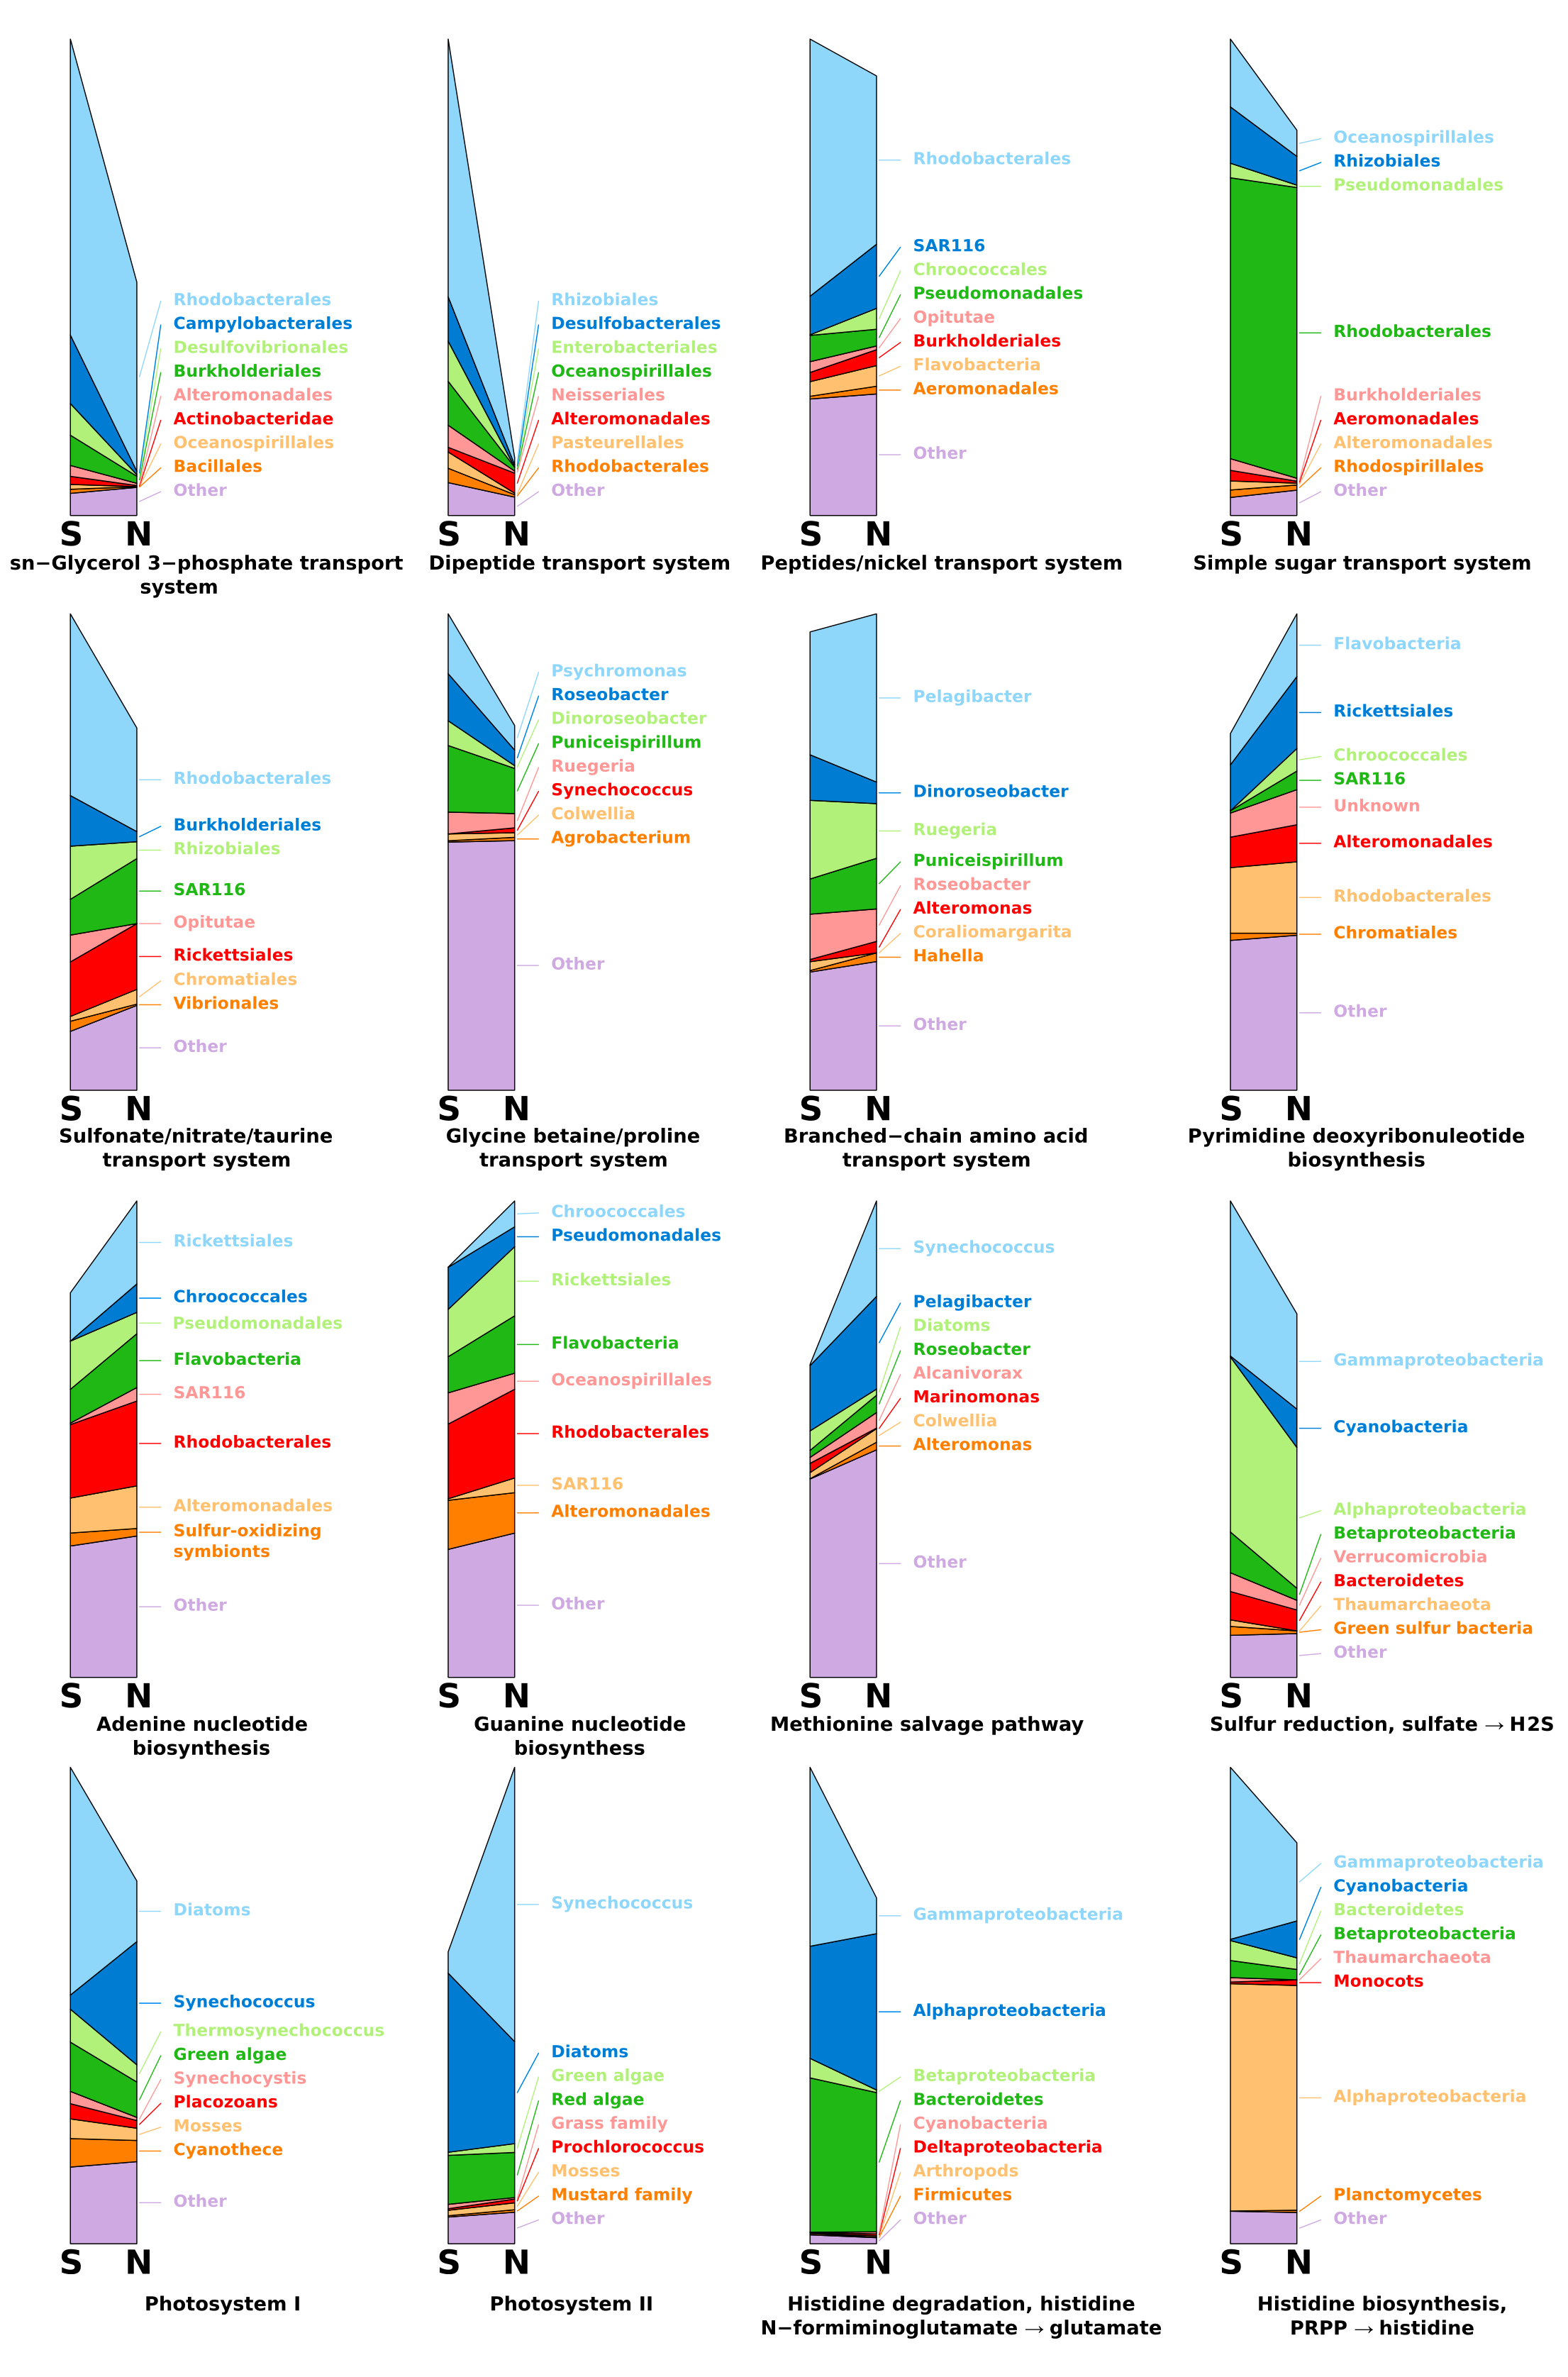
\includegraphics[width=\textwidth]{../polarfront/moduledecomp.png}
  \captionof{figure}[Taxonomic decomposition of KEGG modules]{Decomposition of KEGG modules of interest to contributing classes, orders or genera. The left side of each stack (S) indicates the proportion of the module abundance contributed by each class, order or genus in the South Zone, while the right side (N) represents the North Zone. As the contributions are relative and represent unitless module abundances, no axis is given and proportions are not comparable between modules. Contributing classes, orders or genera are arranged in descending order of the difference in the relative contributions between the zones. Only the eight highest contributors for each module are shown, with the remainder collapsed into the ``Other'' group. The taxonomic ranks to which each module was decomposed are as follows: sn-glycerol 3-phosphate transport, peptide-nickel transport, simple sugar transport and sulfonate/nitrate/taurine transport were decomposed to order; glycine betaine/proline transport and branched-chain amino acid transport to genus; pyrimidine deoxyribonucleotide biosynthesis, adenine nucleotide biosynthesis and guanine nucleotide biosynthesis to order; methionine salvage to genus; sulphur reduction to class; photosystem I and photosystem II to genus; histidine degradation to glutamate and histidine biosynthesis to class.\\
  \rule[1ex]{2cm}{0.5pt}
  }
  \label{fig:moduledecomp}
}


The glycine betaine/proline transport module was also overrepresented in the \ac{SZ}, though this probably reflects glycine betaine's role as an osmo- and cryoprotectant in the colder \ac{SZ} waters.
This is supported by the major taxonomic contributor to this module, genus \genus{Psychromonas}, which includes several psychrophilic species. 

One exception to this pattern was the branched-chain amino acid transport system module, overrepresented in the \ac{NZ}. 
The genera \genus{Pelagibacter} and \genus{Puniceispirillum} were major contributors to this module's overabundance in the \ac{NZ} \figref{fig:moduledecomp}.
As both SAR11 \cite{Giovannoni:2005ib} and SAR116 \cite{Grote:2011dm} representatives encode branched-chain amino acid transporters, the abundance of this module is likely to represent taxonomic differences between the zones.

Biosynthesis pathways for all major nucleic acids (pyrimidine deoxyribonucleotide biosynthesis, adenine nucleotide biosynthesis, guanine nucleotide biosynthesis) were consistently high contributors to variance and overabundant in the \ac{NZ}.
This pattern seems inconsistent with the more oligotrophic nature of the \ac{NZ}, as oligotrophic cells generally have smaller genomes \cite{Lauro:2009gx} and slower growth rates than copiotrophs, and would therefore be expected to require a lower rate of de novo nucleotide biosynthesis.
A possible explanation for this is that \ac{SZ} cells have higher availability of extracellular DNA as a byproduct of decaying phytoplankton \cite{Lomas:2011bp}, which can be imported and salvaged for nucleic acids \cite{Paul:1988wn} thus reducing the requirement for de novo synthesis.
No single taxonomic group contributed a large fraction of the difference in this module \figref{fig:moduledecomp}, suggesting this is a widespread adaptation.

The methionine salvage pathway module had a large contribution to variance between the zones and was overrepresented north of the \ac{PF}.
This may reflect the higher availability of \ac{DMSP} in the \ac{SZ} as a byproduct of blooming eukaryotic algae.
\ac{DMSP} is a major carbon and sulfur source for marine microorganisms, and is commonly assimilated by bacteria through demethylation to \ac{MMPA}, followed by further catabolism to the climatically important compounds dimethylsulfide or methanethiol \citep[review in][]{Curson:2011ic}.
However, when \ac{DMSP} is scarce, \ac{MMPA} may be derived from methionine through the alternative methionine salvage pathway \cite{Reisch:2012bb}.
The genus \genus{Synechococcus}, a noted contributor to marine \ac{DMSP} uptake and assimilation \cite{VilaCosta:2006gt}, was a very high contributor to the abundance of this module in the \ac{NZ} \figref{fig:moduledecomp}, suggesting \genus{Synechococcus} species may use this route when \ac{DMSP} is unavailable.

The sulfur reduction module was overrepresented in the \ac{SZ}, and it is likely that this result is strongly driven by taxonomic differences.
While the taxonomic breakdown indicated a large number of genera contributed to the difference, the Gammaproteobacteria were the highest-contributing class \figref{fig:moduledecomp}.
This module also includes the assimilatory sulfate reduction pathway, which is widespread in marine bacteria, but is absent from SAR11, with known representatives reported to lack genes for assimilatory sulfate reduction (cysDNCHIJ) \cite{Tripp:2008dd}.
The higher relative abundance of SAR11 in the \ac{NZ} may therefore contribute to the lower abundance of genes for assimilatory sulfate reduction in that zone. 

The sulfur reduction module also included adenylylsulfate reductase (APS reductase, encoded by aprAB), an enzyme implicated in sulfite detoxification during heterotrophic growth on organosulfonates \cite{Meyer:2007jd} (N.B. in recent \ac{KEGG} releases, aprA is no longer included in this module).
As the GSO-EOSA-1 representative SUP05 has been found to encode APS reductase, the overabundance of this module may reflect sulfur oxidation through the reverse dissimilatory sulfate reduction pathway \cite{Walsh:2009fja}.
Also, Roseobacter clade bacteria are involved in the decomposition of abundant organic sulfur compounds (e.g.\ \ac{DMSP}, organosulfonates), and hence have been accorded an important role in marine sulfur cycling \cite{Moran:2007fs}.

The photosystem II module was overrepresented in the \ac{NZ}.
Given the underrepresentation of cyanobacterial \acp{OTU} in the \ac{SZ}, this may reflect a dominance of primary production by eukaryotic algae south of the \ac{PF} and cyanobacteria to the north.
Decomposition of the taxonomic affiliations of ortholog groups contributing to this module found \acp{OTU} of \genus{Synechococcus} and \genus{Prochlorococcus} to be major contributors to the difference \figref{fig:moduledecomp}.
Variation in the photosystem I module, which was marginally overrepresented in the \ac{SZ}, could largely be attributed to diatoms and other eukaryotic phytoplankton \figref{fig:moduledecomp}, again supporting a dominance of eukaryotic phytoplankton in \ac{SZ} primary production.
Diatoms have previously been reported at higher abundance south of the \ac{PF}, and their distribution is likely to be linked to the higher concentration of dissolved silica in that region \cite{Trull:2001tg}.
As both eukaryotic phytoplankton and cyanobacteria would be expected to encode both complete photosystems, the differences in module abundance probably reflect the degree of similarity between the photosystem I and II genes in the \ac{KEGG} database and those found in the sampled environments. 

The histidine degradation to glutamate module, which comprises four ortholog groups mediating the degradation of histidine to glutamate via N-formiminoglutamate, was overrepresented in the \ac{SZ}.
The histidine biosynthesis module was also overrepresented in the \ac{SZ}.
While the concentration of dissolved histidine in the \ac{SO} is generally low \cite{Kawahata:2000ur}, blooming eukaryotic phytoplankton (which are more prevalent in the \ac{SZ}) may deplete nitrate while releasing \ac{DFAA}.
As \ac{DFAA} become available, they are used by bacteria to sense the decaying bloom. 
Histidine may therefore act as a proxy for \ac{DFAA} to regulate the expression of bacterial aminopeptidases, which are involved in lysing diatoms \cite{Bidle:2001vi}.
The class Bacteroidetes, while a small contributor to the histidine biosynthesis module in the \ac{SZ}, was a large contributor to histidine degradation \figref{fig:moduledecomp}, supporting an association between Bacteroidetes and phytoplanktonic bloom products. 
It is also possible that uptake and degradation of histidine to glutamate (which generates ammonia as a by-product) may function as a limited nitrogen source.

\subsubsection{Conclusions: Biogeographic role of the Polar Front}

These results show that there are major taxonomic and functional differences across the \ac{PF}.
The differences in functional potential between the \ac{NZ} and \ac{SZ} reflect both their taxonomic profiles and fundamental trophic and ecological differences.
In particular, they provide genomic support that the \ac{NZ} is more oligotrophic than the \ac{SZ} \cite{Pollard:2002vr,Giovannoni:2005ib,Alonso:2006dj,Lauro:2009gx}, and are consistent with the observation that primary production is higher south of the \ac{PF} \cite{Strutton:2000ta,Williams:2010jy}.
Our findings extend previous work in defining the \ac{PF} as a strong biogeographic boundary which shapes not only the composition, but also the functional capacity of microbial communities in the \ac{SO}.

These results do not exclude the possibility that other major \ac{SO} fronts, particularly the \ac{STF} and \ac{SAF}, are also significant biogeographic boundaries, as has been reported in some previous reports for specific taxonomic groups \citep[e.g.][]{Abell:2005ji}.
While the sampling resolution in this study was not sufficient to resolve the effects of other fronts, there are some indications in the data of further structure within the zones.
The two samples north of the \ac{STF} had significantly larger cyanobacterial populations than the remaining \ac{NZ} samples (see discussion of \genus{Prochlorococcus} and \genus{Synechococcus}, above).
Future sampling across these fronts at higher resolution will provide the data necessary to investigate finer biogeographic patterns.

The nature and function of microbial communities in the \ac{SO} are of global significance.
Knowledge of these communities and their biogeographic drivers has relevance for understanding and predicting the long-term effects of climate change.
These findings provide a basis for predicting how climate change-driven shifts in the \ac{SO} may affect microbial communities; in particular, the effects of changes in the nature and location of the \ac{ACC} on the ecosystem functions of \ac{SO} microorganisms.


%reset acronyms
\glsresetall
\chapter[Deep water formation]{Transport of microbial cells during deep water formation}
\label{ch:deepwaterformation}

\section{Abstract}

During sampling for the study presented in \secreft{ch:polarfront}, additional samples were collected of \ac{AABW} on the Antarctic continental shelf and from the sea floor in the vicinity of the mid-ocean ridge.
Metagenomic analysis found that the community composition of the continental shelf samples was surprisingly similar to that of surface samples in the same area, despite the significant differences in environmental factors such as pressure and light availability.
This may have resulted from the rapid advection of cells in the sinking of surface waters to form \ac{AABW} (deep water formation; see \secreft{ch:intro}).
These results led to the study described in \secreft{ch:advection}.

\section{Introduction}

The Mertz Glacier polynya is a region of open ocean (bound by the Antarctic coast, sea ice and the Mertz glacier tongue) west of the Mertz Glacier tongue (approx. 67\textdegree{} S, 145\textdegree{} E).
The polynya has historically been a major site for the formation of \ac{AABW} in the \ac{SO}, although its role in this process has become less clear following the calving of a large section of the glacier tongue in February 2010 \cite{Tamura:2012da}.
Evaporative cooling of the sea surface by katabatic winds from the Antarctic continent, combined with the exclusion of salt from forming sea ice (``brine exclusion'' or ``brine rejection''), results in the rapid formation and sinking of cold, dense water \cite{Williams:2008iu}.
This water forms an abyssal layer in the Ad\'{e}lie depression (a bathymetric feature underlying the polynya), eventually outflowing northwards over the continental sill as part of the \ac{AABW}.

This brief chapter presents an exploratory analysis of two abyssal samples of \ac{AABW} from within the Ad\'{e}lie depression, and one from the South Australian basin further north.
The results from this study led to the investigation of advective transport of microorganisms described in \secreft{ch:advection}.

\section{Methods}

\begin{table}
\sffamily
\footnotesize
\caption[\ac{AABW} samples used in the preliminary analysis]{Sampling time, location and physicochemical properties of \ac{AABW} samples used in this preliminary study.
All data were retrieved from the \ac{CTD} (SeaBird, Bellevue, USA) instrument used to collect the samples.}
\label{tab:deepsamples}
\begin{tabu} to\textwidth{llllIZXX}
\toprule
\textbf{Sample} & \textbf{Date} & \textbf{Latitude} & \textbf{Longitude} & \textbf{Depth (m)} & \textbf{Temperature (\textdegree{}C)} & \textbf{Salinity (PSU)} & \textbf{Volume \linebreak filtered (L)}\\
\midrule
356 & 03/01/2008 & \textminus{}66.76 & 144.41 & 920 & -1.9 & 34.69 & 230\\
361 & 14/01/2008 & \textminus{}66.47 & 140.56 & 1170 & -1.8 & 34.56 & 225\\
365 & 23/01/2008 & \textminus{}56.70 & 141.91 & 3693 & 0.5 & 34.69 & 230\\
\bottomrule
\end{tabu}
\end{table}

% the sample map
\begin{figure}
  \centering
  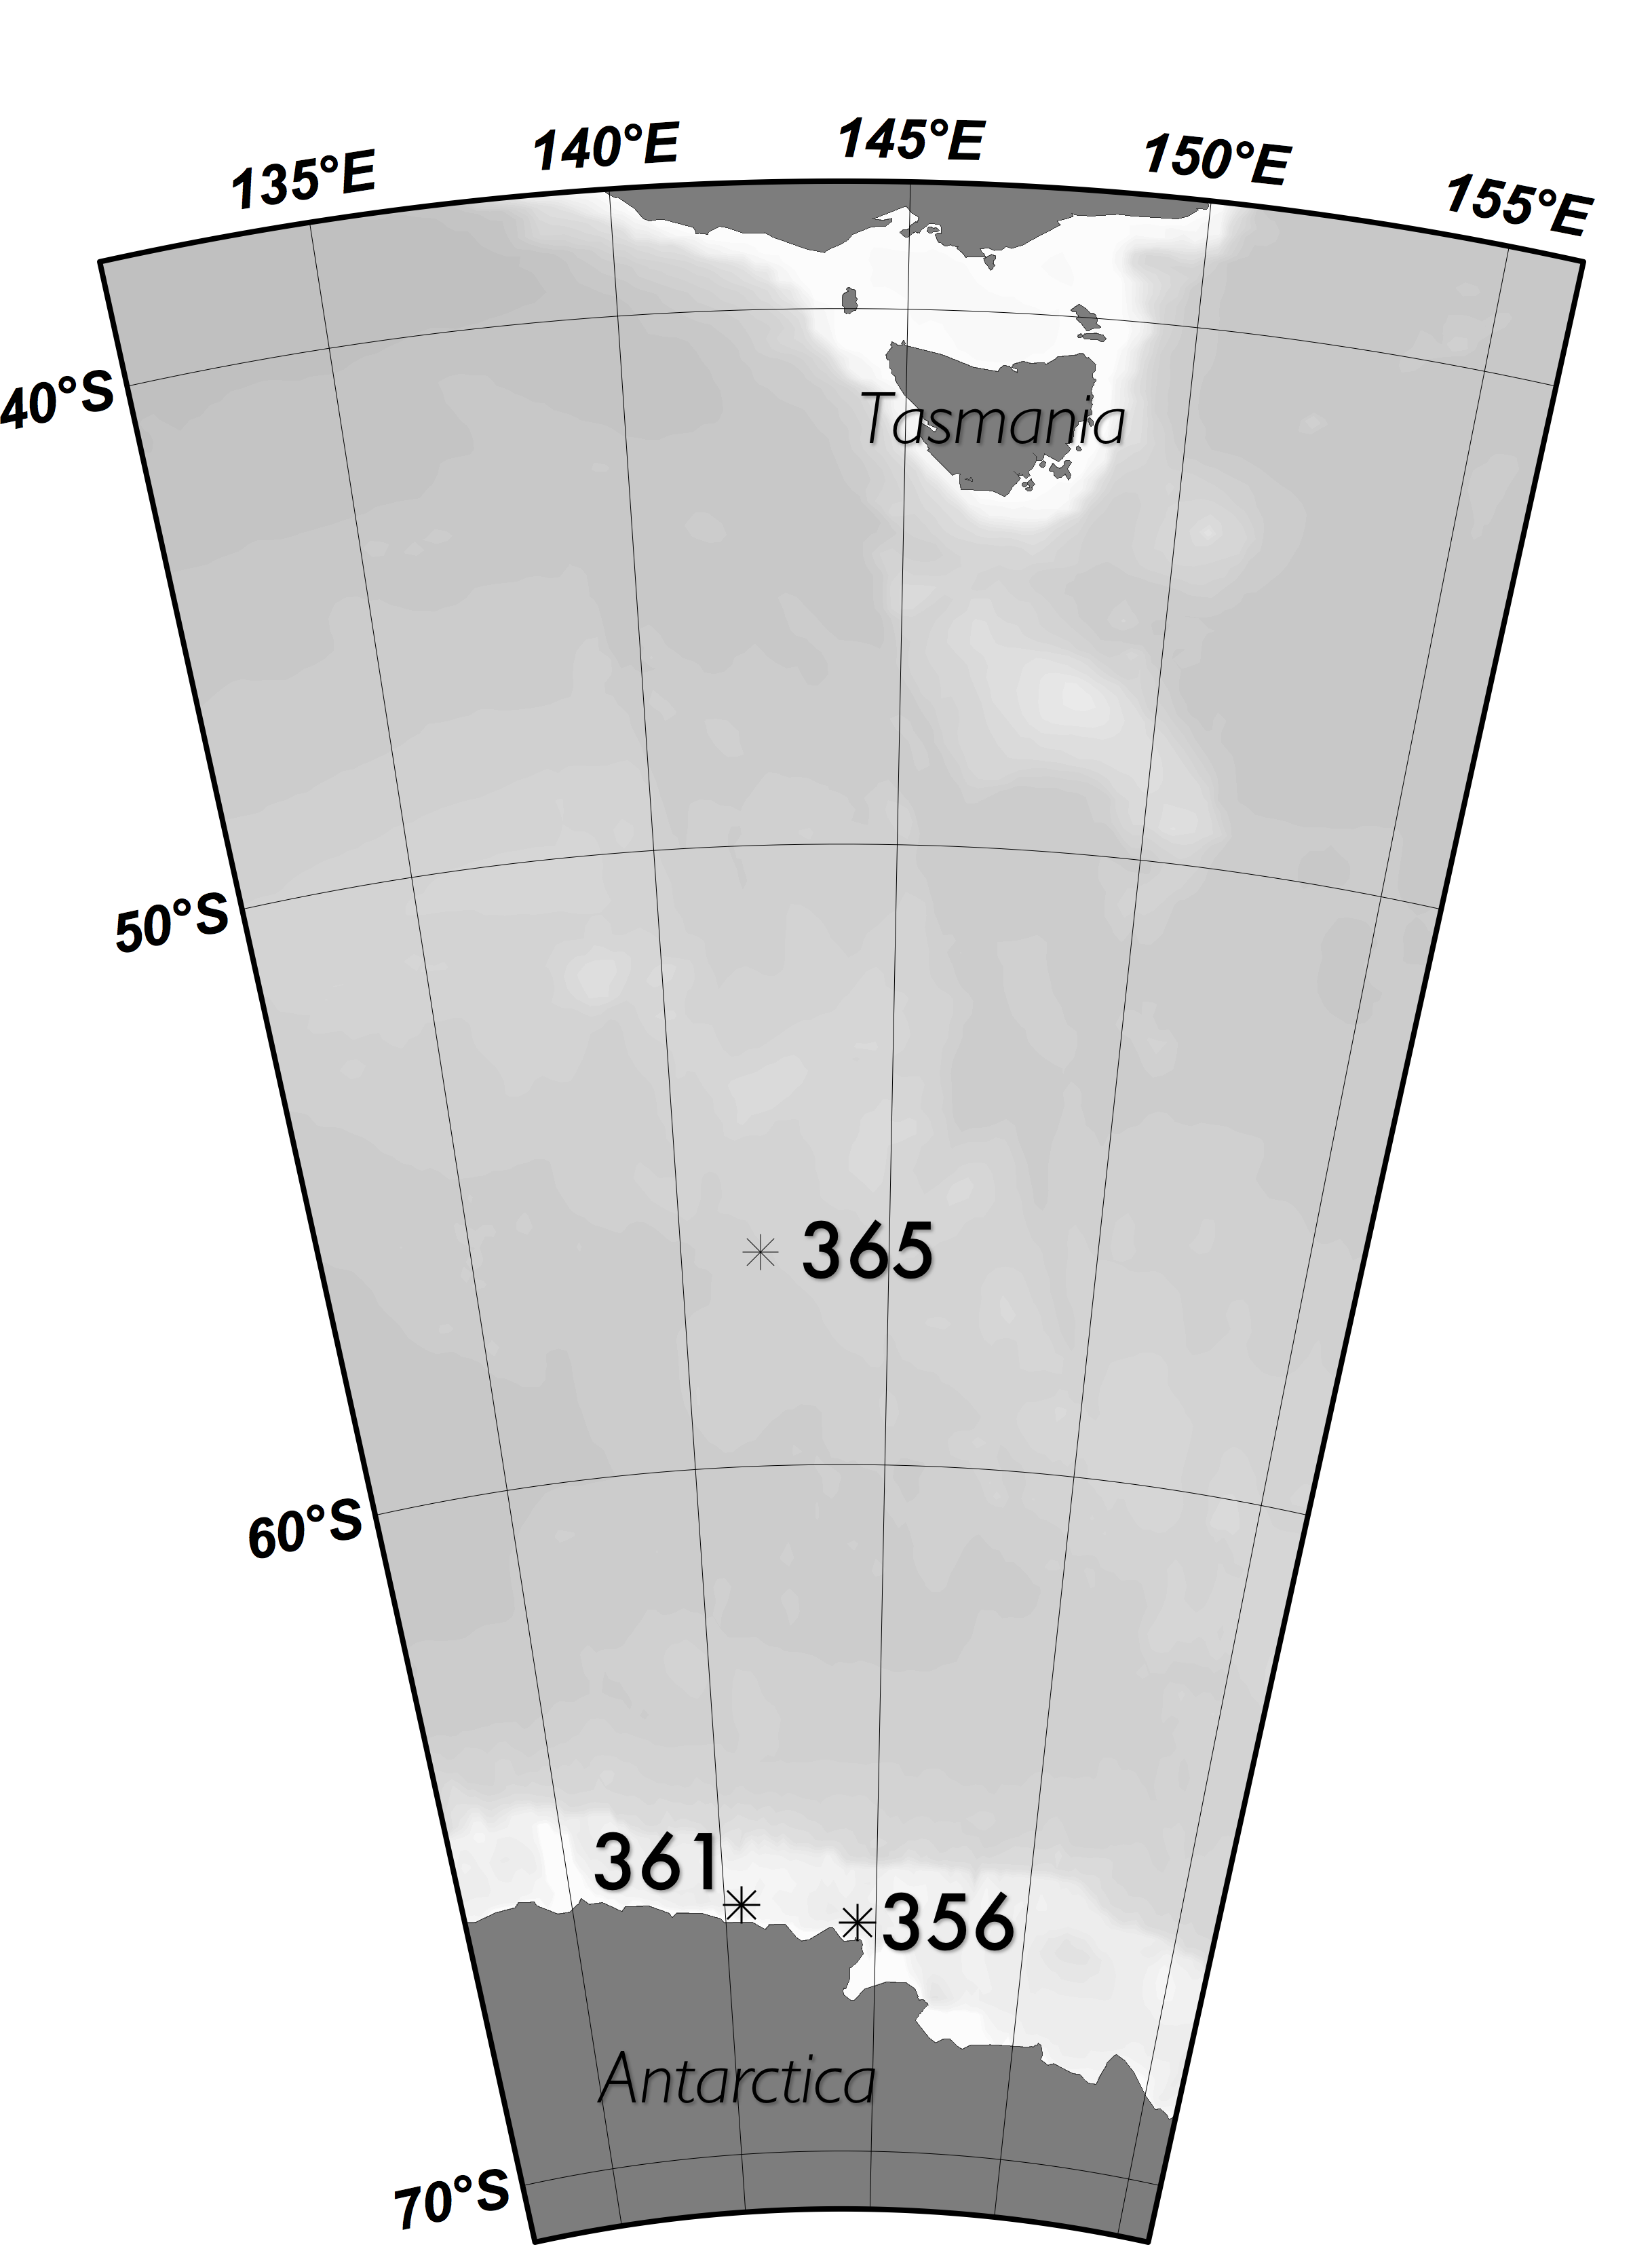
\includegraphics[width=\textwidth]{../deepwaterformation/deepsamplemap.png}
  \caption[Map showing sites of preliminary \ac{AABW} samples]{Sites of preliminary \ac{AABW} samples.}
  \label{fig:deepsamplemap}
\end{figure}


Three samples of \ac{AABW} were opportunistically obtained and analysed during the project described in \secreft{ch:polarfront} \figref{fig:deepsamplemap}.
Two of these samples (356 and 361) were of newly formed \ac{AABW} waters on the Antarctic continental shelf, while one (365) was of abyssal \ac{AABW} from the South Australian basin \tabref{tab:deepsamples}.
DNA extraction, sequencing and construction of a taxonomic profile by \softwarename{blast} comparison to the RefSeq database and processing with \ac{GAAS} were performed using the methods described in \secreft{ch:polarfront}.
A standardised and log-transformed Bray-Curtis resemblance matrix was constructed including the taxonomic profiles of the \ac{AABW} samples as well as the \ac{NZ} and \ac{SZ} samples described in \secreft{ch:polarfront}.
A \ac{nMDS} plot was then constructed from this matrix.
All statistical procedures were performed in \softwarename{PRIMER 6} as described by \citet{Clarke:2001ut}.

\section{Results and Discussion}

Although the three \ac{AABW} samples were taken in deep, cold and aphotic waters \tabref{tab:deepsamples} compared to the surface \ac{AZ} and \ac{SZ} samples, the \ac{nMDS} plot suggested that the two continental shelf \ac{AABW} samples (356 and 361) were surprisingly similar to those of the \ac{AZ}, particularly sample 353 \figref{fig:deepnmds}.
Further, the indicated the presence of several \acp{OTU} which would not be expected to be present at significant abundance in deep, aphotic waters \tabref{tab:topdeepotus}.
For example, \species{Roseobacter denitrificans} OCh 114, a model organism for aerobic anoxygenic photosynthesis, was the fifth most abundant \ac{OTU} of the continental shelf samples.
Numerous \ac{CFB} representatives, typically associated with \ac{POM} and the utilisation of \ac{HMW} phytoplankton products \citep[e.g.][]{Williams:2012gsa}, were also unexpectedly high.

\begin{landscape}
\begin{table}
\centering
\sffamily
\caption[Twenty most abundant \acp{OTU} in preliminary \ac{AABW} samples]{Relative abundances (as percentages) of the twenty most abundant \acp{OTU} identified in the preliminary study of \ac{AABW} samples.}
\label{tab:topdeepotus}
\begin{tabular}{lS[table-format=2.5]S[table-format=2.5]S[table-format=2.5]S[table-format=2.5]S[table-format=2.5]S[table-format=2.5]}
\toprule
\textbf{OTU} & \multicolumn{3}{c}{\textbf{Sample 356}} & \multicolumn{3}{c}{\textbf{Sample 365}}\\
\cmidrule(r){2-4}
\cmidrule(r){5-7}
& {0.1 \micron} & {0.8 \micron} & {3.0 \micron} & {0.1 \micron} & {0.8 \micron} & {3.0 \micron}\\
\midrule
\candidatusfull{Pelagibacter ubique} HTCC1062 & 48.40 & 32.32 & 32.85 & 19.02 & 22.31 & 3.880\\
\speciesfull{Nitrosopumilus maritimus} SCM1 & 11.92 & 9.289 & 13.99 & 30.17 & 7.790 & 22.74\\
\candidatusfull{Ruthia magnifica} str. Cm (\species{Calyptogena magnifica}) & 3.780 & 4.563 & 2.356 & 2.844 & 1.504 & 0.2599\\
\candidatusfull{Vesicomyosocius okutanii} strain HA & 2.349 & 2.757 & 1.396 & 1.859 & 0.8025 & 0.08227\\
\genus{Roseobacter} sp. OCh 114 & 0.1412 & 1.166 & 0.6845 & 0.08564 & 0.6662 & 0.4851\\
\candidatusfull{Puniceispirillum marinum} IMCC1322 & 0.3180 & 1.103 & 0.6403 & 0.4218 & 0.8223 & 0.4202\\
\species{Marinobacter hydrocarbonoclasticus} VT8 & 0.06999 & 0.4091 & 0.3976 & 0.2476 & 1.050 & 2.338\\
\species{Silicibacter pomeroyi} DSS-3 & 0.1081 & 0.8406 & 0.4996 & 0.1290 & 0.4630 & 0.3621\\
\species{Robiginitalea biformata} strain HTCC2501 & 0.2813 & 0.6433 & 0.7417 & 0.1769 & 0.2739 & 0.4978\\
\species{Pseudoalteromonas haloplanktis} strain TAC125 & 0.02530 & 0.4540 & 0.1958 & 0.2836 & 2.817 & 0\\
\species{Alcanivorax borkumensis} strain SK2 & 0.09262 & 0.3163 & 0.4281 & 0.1049 & 0.5674 & 1.985\\
\species{Gramella forsetii} strain KT0803 & 0.3096 & 0.6465 & 0.7405 & 0.1254 & 0.2670 & 0\\
\genus{Colwellia} sp. 34H & 0.04289 & 0.4512 & 1.020 & 0.07200 & 0.4532 & 0.7727\\
\species{Flavobacterium psychrophilum} strain JIP02/86 & 0.2417 & 0.4722 & 0.6353 & 0.07943 & 0.1645 & 0.5072\\
\species{Pirellula staleyi} strain DSM 6068 & 0.003149 & 0.2477 & 0.3093 & 0.08767 & 1.401 & 0.7732\\
\genus{Jannaschia} sp. DFL-12 & 0.07995 & 0.6770 & 0.3841 & 0.03865 & 0.2030 & 0.1025\\
\species{Pseudoalteromonas atlantica} strain T6c & 0.02312 & 0.1653 & 0.1941 & 0.03856 & 0.3235 & 1.728\\
\species{Zunongwangia profunda} strain SM-A87 & 0.1830 & 0.3499 & 0.4826 & 0.1036 & 0.1362 & 0.3825\\
\genus{Silicibacter} sp. TM1040 & 0.09568 & 0.5448 & 0.3455 & 0.03477 & 0.2014 & 0.1740\\
\species{Capnocytophaga ochracea} strain DSM 7271 & 0.1251 & 0.2916 & 0.4491 & 0.03893 & 0.1542 & 0.5332\\
\bottomrule
\end{tabular}
\end{table}
\end{landscape}


A possible explanation for these observations is that the continental shelf samples represent \ac{AABW} recently formed in the D'Urville sea, and the observed assemblage therefore represents advection rather than selection by environmental factors.
The project described in \secreft{ch:advection} was designed to test and explore this hypothesis.

\begin{figure}[!ht]
  \centering
  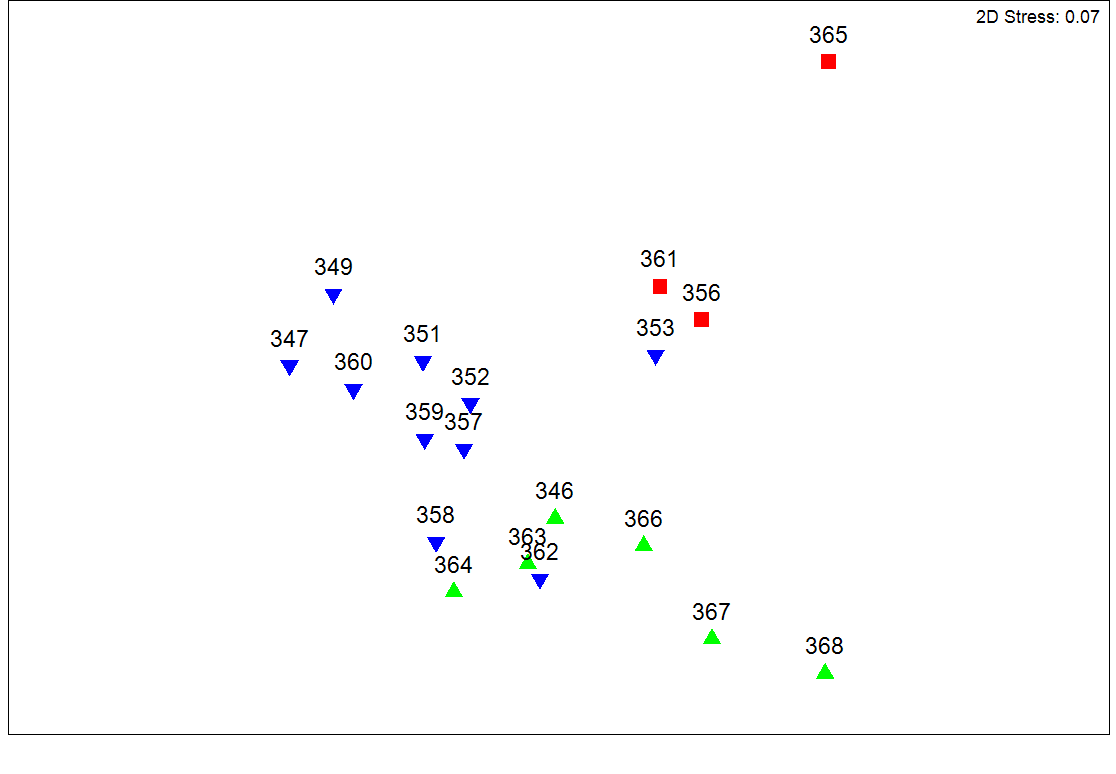
\includegraphics[width=\textwidth]{../deepwaterformation/deepnmds.png}
  \caption[\ac{nMDS} of \ac{AABW}, \ac{NZ} and \ac{SZ} samples]{\ac{nMDS} plot showing distance between \ac{AABW}, \ac{NZ} and \ac{SZ} samples.
  Green triangles represent samples from the \ac{NZ}; blue inverted triangles from the \ac{SZ}; and red squares from \ac{AABW}.}
  \label{fig:deepnmds}
\end{figure}



%reset acronyms
\glsresetall
\chapter[The advection effect]{The advection effect as a driver of microbial biogeography}
\label{ch:advection}

\previouslypublished{Sections of this chapter have been previously published in}

\section{Abstract}

The distribution and abundance of marine microbes are shaped by environmental factors and spatial separation.
The physical transport of cells by ocean currents (advection) is also frequently invoked when describing marine microbial biogeography, but the role of advection has never been directly confirmed or measured.
In this study, the microbial communities at 25 sites in the Southern Ocean were sampled and compared to a model of particle advection between the sites.
Even when environmental factors and spatial separation were controlled for, the ``advection effect'' explained 7\% of variation in community composition.
Further investigation confirmed that this effect was directional, and likely represented an increase in the colonisation of distant sites by small numbers of cells.
This study provides further evidence that microbial dispersal potential is far from total, and supports the role of ocean currents in shaping marine microbial ecosystems.

\section{Introduction}

The central goal of microbial biogeography is to understand how the distribution and abundance of microorganisms are shaped by their physical context.
The Baas Becking hypothesis --- that ``\textit{everything is everywhere}, but, \textit{the environment selects} \cite{Becking:1934um, deWit:2006de}'' --- posits that the rapid dispersal of microorganisms means microbial community structure is determined entirely by environmental selection.
This stands in contrast to macroorganism biogeography, which has long been recognised as being under the control of historical (in addition to contemporary environmental) factors, particularly spatial influences such as barriers to dispersal.
Microbial biogeography studies have begun to show that historical factors may also shape the distribution of microorganisms \cite{Martiny:2006jy}, e.g.\ a correlation between spatial and genetic distance (a ``distance effect'') in fluorescent \genus{Pseudomonas} strains in soils \cite{Cho:2000tn}.
This study, among others \cite{Ramette:2007bb,Storch:2008tq}, also demonstrated the importance of taxonomic resolution in describing such biogeographic patterns.
Other studies have found that dispersal potential varies between microbial species, leading to different or absent distance effects \cite{Bissett:2010wj}.
When combined with contemporary environmental selection (``environment effect''), distance effects explain some but not all variation between microbial communities, and the mechanism(s) by which a distance effect arises are not always clear \cite{Hanson:2012cb}.

In the ocean, several recent studies have found that microbial communities can be endemic to hydrographically distinct water masses.
Surveys in the Arctic \cite{Galand:2009hy} and North Atlantic \cite{Agogue:2011fm} oceans have found that bacterial assemblages within the same water mass can be similar across a range of thousands of kilometres, but assemblages can differ between water masses across a range of hundreds of meters.
Water masses are defined by their distinct physicochemical properties, so such patterns do not directly imply the existence of factors beyond environmental selection.
However, in some cases a water mass-community relationship has been shown to persist even when environment effects are statistically controlled for \cite{Hamilton:2008tp, Hamdan:2013ko}.

During the study on the biogeographic effect of the \ac{PF} described earlier in this volume, it was found that microbial communities in surface waters of the Mertz Glacier region, a site of deep water formation, were very similar to those at the bottom of the water column, despite the very different environmental conditions (see \secreft{ch:deepappendix}).
One hypothesis explaining both this observation and water mass endemicity is that microbial assemblages are influenced by the advection (physical transport) of cells by ocean currents. 
Higher dispersal rates cause the microbial community composition at a given site to increasingly resemble the dispersed colonisers, and less reflect local environmental selection and stochastic effects such as genetic drift \cite{Hanson:2012cb}.
Hence, it would be expected that locations that are closely connected by advection (e.g.\ those within the same water mass, or different levels of the water column at a site of deep water formation) would have more similar compositions than those that are not, even when the environment effect is accounted for.
Indeed, advection is often invoked to explain observations of microbial diversity or abundance which do not seem attributable to environmental selection \citep[e.g.][]{Sul:2013in, Ghiglione:2012ei, Giebel:2009hr, Lauro:2007bf}.
The exchange of very small volumes of water between marine microbial mesocosms has been found to greatly reduce their \textbeta-diversity even under consistent environmental conditions \cite{Declerck:2013cz}.
This suggests that advection of even small numbers of cells could have a large homogenizing effect independent of environmental selection.
However, the existence of a relationship between advection and community composition that is independent of environment and distance effects has not been directly tested.

The \ac{SO} is composed of several water masses, which are physicochemically distinct but linked by circulation (see \secreft{ch:intro} for a full description; see also \figreft{fig:advectionsamplemap}).
This study aimed to determine whether advection shapes the community structure of bacteria and archaea, independent of environment and distance effects.
By sampling each of the \ac{SO} water masses (depths from surface to \textapprox{}6 km), dissimilarity between microbial communities over a large spatial distance (\textapprox{}3000 km) and range of environments could be determined, in order to test whether advection played a role in shaping their composition.

\section{Methods}

\subsection{Sampling}

\begin{figure}
  \centering
  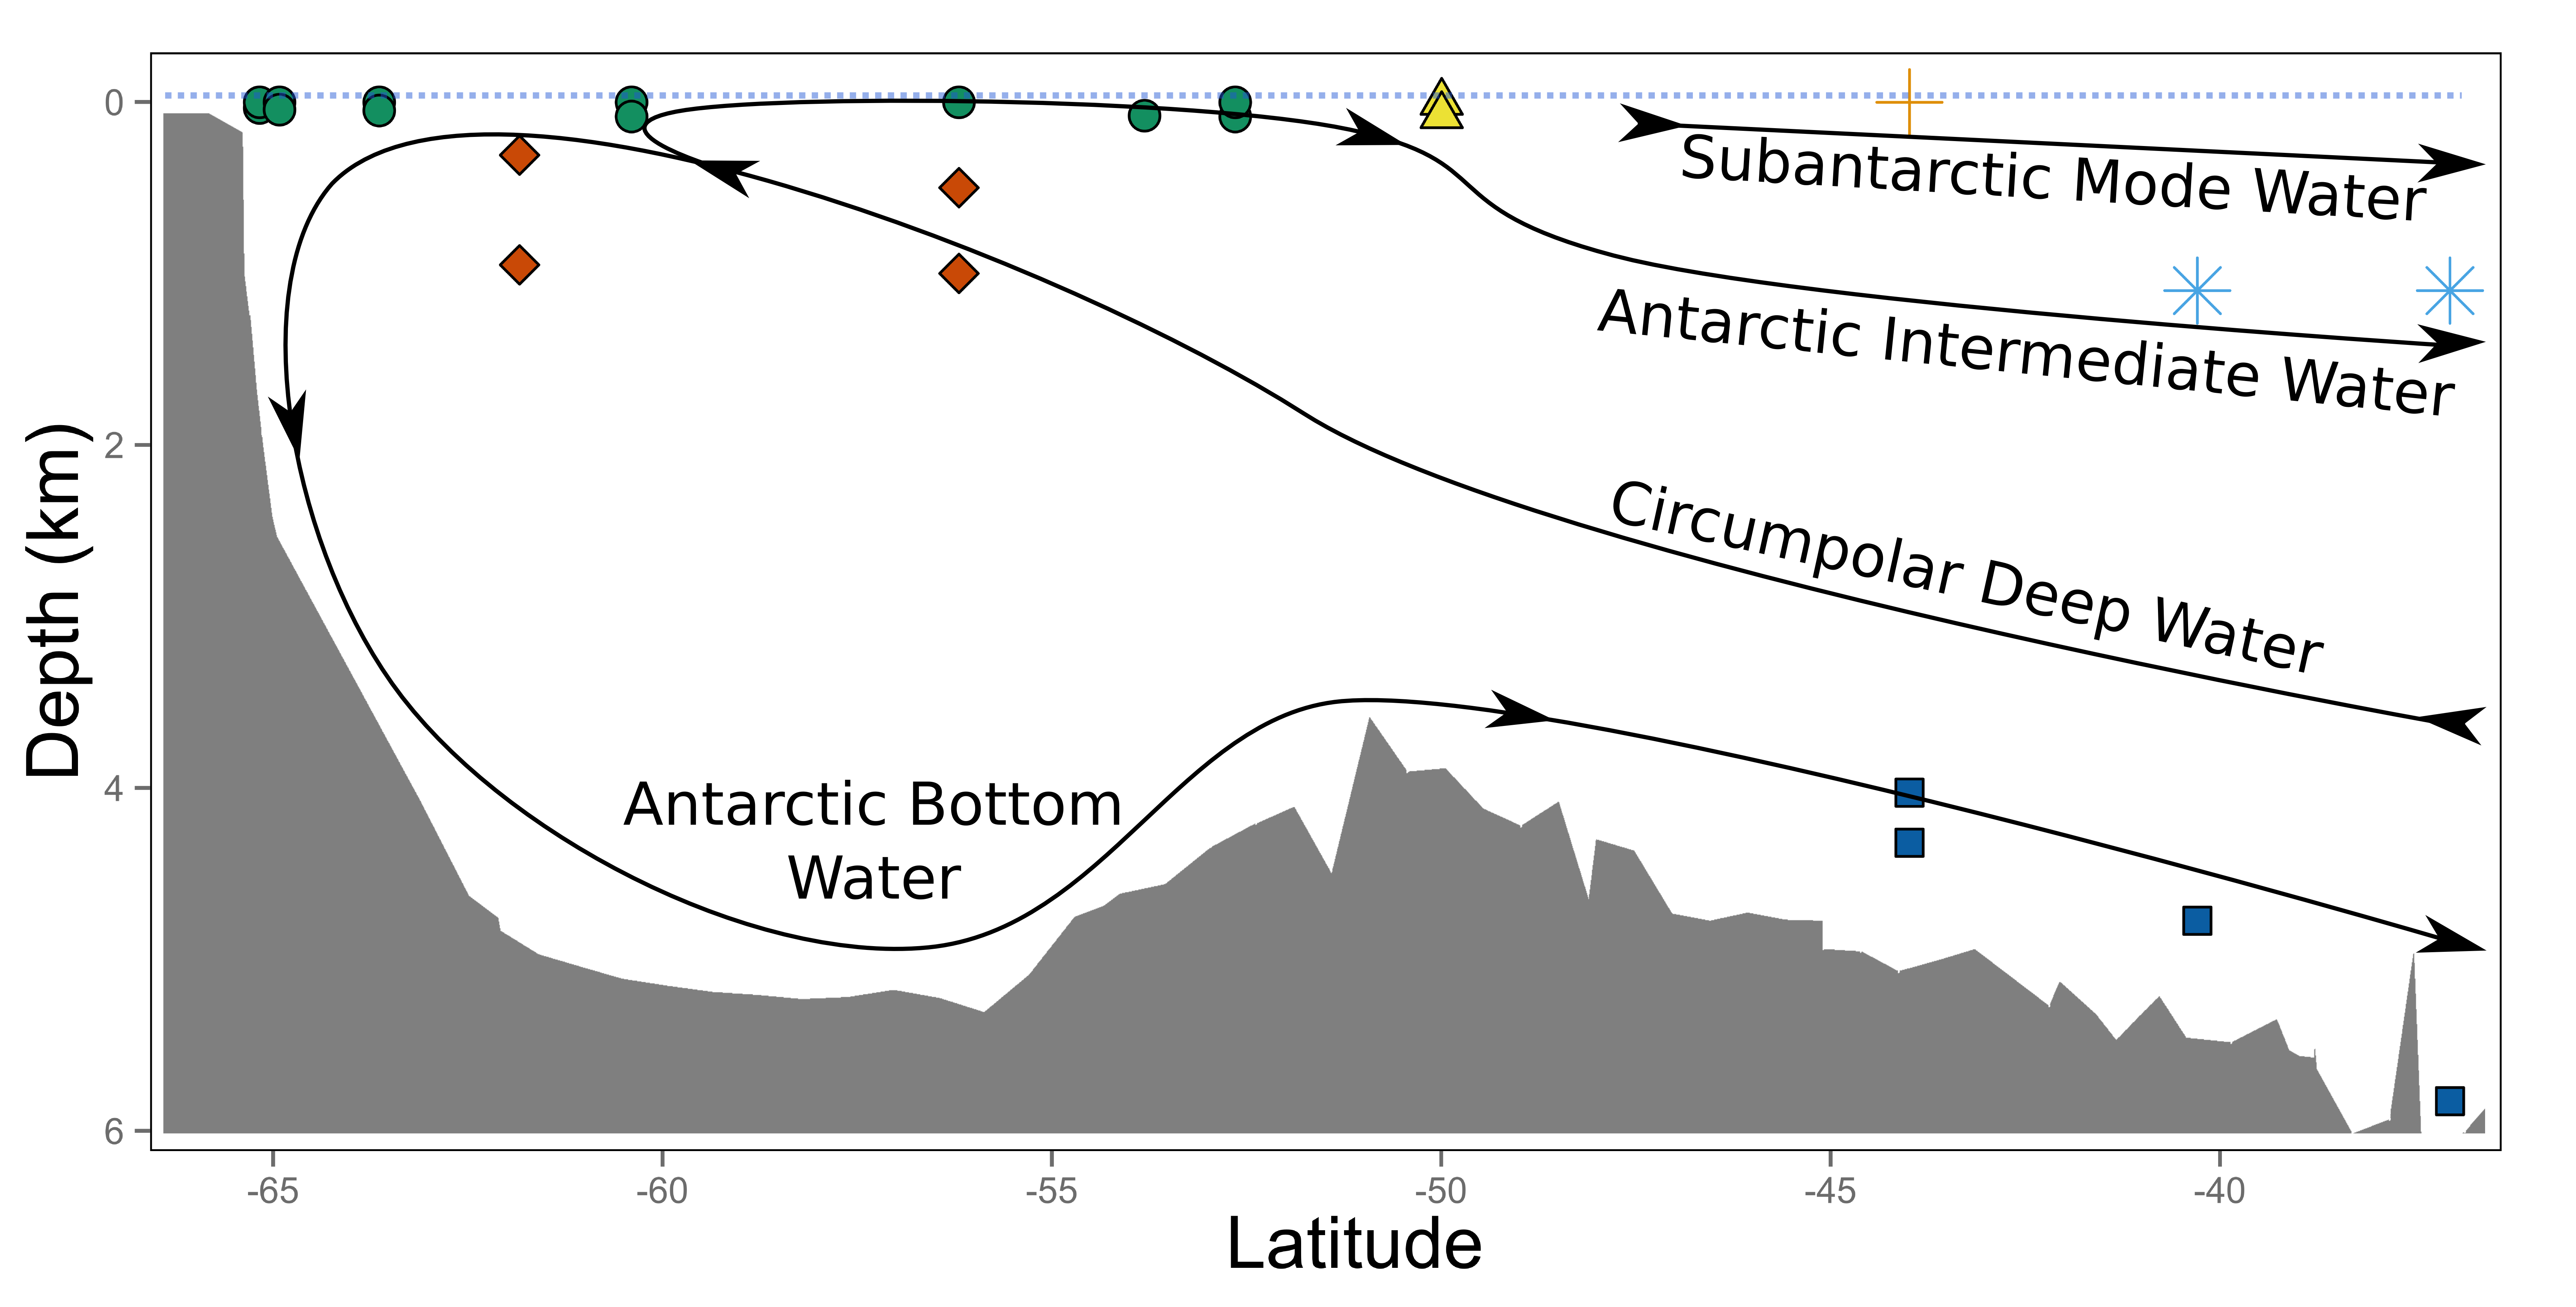
\includegraphics[width=\textwidth]{../advection/advectionsamplemap.png}
  \caption[Map showing sites of samples used in the advection study]{Antarctic Intermediate Waters (AAIW), light blue stars; Subantarctic Mode Water (SAMW), orange crosses; Antarctic Bottom Water (AABW), dark blue squares; Antarctic Zone (AZ), green circles; Polar Frontal Zone (PFZ), yellow triangles; Circumpolar Deep Water (CDW), red diamonds; sea surface, blue dashed horizontal line. Bathymetry is an approximate representation for 115\textdegree{} E, and is indicative only.}
  \label{fig:advectionsamplemap}
\end{figure}

Sampling\footnote{Sampling was performed by David Wilkins, Timothy J.\ Williams and Sheree Yau.} was conducted on board the RSV \textit{Aurora Australis} during cruise V3 from January 20th--February 7th 2012.
This cruise occupied a latitudinal transect from waters north of Cape Poinsett, Antarctica (65\textdegree{} S) to south of Cape Leeuwin, Australia (37\textdegree{} S) within a longitudinal range of 113--115\textdegree{} E.

Sampling was performed as described in \citet{Wilkins:2012wg}, with sites and depths selected to provide coverage of all major \ac{SO} water masses.
At each surface station, \textapprox{}250--560 L of seawater was pumped from \textapprox{}1.5--2.5 m depth.
At some surface stations, an additional sample was taken from the \ac{DCM}, as determined by chlorophyll fluorescence measurements taken from a \ac{CTD} cast at each station.
Samples of mesopelagic and deeper waters (\textapprox{}120--240 L) were also collected at some stations using Niskin bottles attached to the \ac{CTD}.
Sampling depths were selected based on temperature, salinity and dissolved oxygen profiles to capture water from the targeted water masses.
Profiles were generated on the \ac{CTD} descent, and samples collected on the ascent at the selected depths.
Deep water masses were identified by the following criteria: \ac{CDW} = oxygen minimum (\ac{UCD}) or salinity maximum (\ac{LCD}); \ac{AABW} = deep potential temperature minimum; \ac{AAIW} = salinity minimum \cite{Foldvik:1988gp}.
Surface zones were identified relative to the major fronts of the \ac{SO}, which are marked by strong latitudinal gradients in temperature and salinity \cite{Sokolov:2002tc, Orsi:1995va}.
The \ac{AZ} lies south of the \ac{PF} (\textapprox{}51\textdegree{} S at the time of sampling), while the \ac{PFZ} lies between the \ac{PF} and the \ac{SAF}.
\ac{SAMW} overlays \ac{AAIW} north of the \ac{SAF}.
In total, 25 samples from the \ac{AZ}, \ac{PFZ}, \ac{SAMW}, \ac{AAIW}, \ac{CDW} and \ac{AABW} were collected for this study \figref{fig:advectionsamplemap}.

Seawater samples were prefiltered through a 20 \micron{} plankton net, then filtrate was captured on sequential 3.0 \micron{} 0.8 \micron{} and 0.1 \micron{} 293 mm polyethersulfone membrane filters (Pall, Port Washington, USA), and immediately stored at $-20$ $^\circ$C \cite{Rusch:2007ez,Ng:2010cd}.

\subsection{DNA extraction}

DNA extraction was performed using a modified version of the phenol-chloroform method described in \citet{Rusch:2007ez}.
Samples were thawed in a 37 \textdegree{}C water bath.
Half of the storage buffer (\textapprox{}10 mL) was decanted into a clean 50 mL centrifuge tube.
If the volume decanted was less than 10 mL, the difference was made with sterile water (Sigma-Aldrich, St.\ Louis, USA).
An equal volume of 50\% sucrose lysis buffer (50 mM TRIS-HCl, 40 mM EDTA, 0.75 M Sucrose, pH 8) was added such that the final concentration was 25\% sucrose lysis buffer.
A small pinch of lysozyme (Sigma-Aldrich, St.\ Louis, USA) (final concentration \textapprox{}2.5 mg/mL) and 1 mL TRIS-EDTA (10 mM TRIS, 1 mM EDTA, pH 8) was added.

The filter membrane was removed from the storage tube and cut in half aseptically.
One half was returned to the storage tube, which was refrozen at $-80$ \textdegree{}C.
The remaining half was cut in half again, and one quarter-filter placed atop the other such that the biomass (filtrand) on each piece was facing outwards.
Keeping the filters together, they were cut into very fine (\textapprox{}3 mm by 10 mm) strips, which were placed in the 50 mL centrifuge tube containing the buffer and lysozyme mixture.
This tube was mixed by gentle inversion, then tapped such that all filter strips collected at the bottom of the tube and were covered by lysis buffer.
The tube was then incubated in a 37 \textdegree{}C shaking water bath at 275 RPM for 30--60 min.

200 \microlitre{} of 20 mg/mL Proteinase K (Sigma-Aldrich, St.\ Louis, USA) was added to the tube, which was mixed by gentle inversion.
The tube was gently tapped such that all filter strips collected at the bottom covered by lysis buffer.
The tube was then subjected to three freeze-thaw cycles, each cycle consisting of 20--30 min in a $-80$ \textdegree{}C freezer followed by 20--30 min in a 55 \textdegree{}C water bath.
After the final complete thaw, 200 \microlitre{} of 20 mg/mL Proteinase K and 2 mL of 10\% SDS (Sigma-Aldrich, St.\ Louis, USA) were added to the tube.
The tube was mixed by gentle inversion then gently tapped such that all filter strips collected at the bottom covered by lysis buffer.
It was then incubated in a 55 \textdegree{}C shaking water bath at 175 RPM for two hours.

The supernatant was pipetted from the tube using a genomic tip and split evenly into two new 50 mL centrifuge tubes.
An equal volume of buffer-saturated (10 mM TRIS HCl, 1 mM EDTA, pH 8) phenol (Sigma-Aldrich, St.\ Louis, USA) was added to each of the tubes, which were mixed by gentle inversion.
The mixtures were then fractionated in a fixed-angle rotor centrifuge for 15 min at 3700 RPM at room temperature.
The bottom layer of each tube was removed by pipette into a new 50 mL centrifuge tube.
Each of these two tubes was then made to 50 mL with sterile water (Sigma-Aldrich, St.\ Louis, USA).
After mixing by gentle inversion, each 50 mL mixture was then split evenly into two new 50 mL centrifuge tubes, resulting in four tubes each containing 25 mL of mixture.
These tubes were then made to 50 mL with 1-propanol (Sigma-Aldrich, St.\ Louis, USA).
The mixtures were homogenised by gentle inversion and incubated at 4 \textdegree{}C overnight.

Following incubation, the tubes were centrifuged using a fixed-angle rotor for 30 min at 7500 RPM and room temperature.
The majority of the supernatant was removed by decanting, and the tubes left to sit until the remaining supernatant (\textapprox{}1 mL) collected at the bottom over the precipitated pellet.
The pellet was then resuspended by gentle pipetting with a genomic tip, and the suspension placed in a new 1.5 mL microcentrifuge tube (four tubes total).
These tubes were then centrifuged in a microcentrifuge for 10 minutes at 13,000 RPM and room temperature.
The supernatant was removed by pipette and the tubes placed in a 37 \textdegree{}C heat block with the lids opened and covered by a sterile KimWipe (Kimberly-Clark, Irving, USA) for 10 min, or longer if the supernatant did not evaporate completely in that time.
93.75 \microlitre{} of TRIS-EDTA was added to each tube, and the tubes were incubated at 4 \textdegree{}C for one hour to allow the DNA pellet to redissolve.

After this incubation, the pellets were gently pipetted with a genomic tip to ensure complete resuspension.
The suspensions from all four tubes were combined, and an additional 750 \microlitre{} of TRIS-EDTA added.
This was then split evenly into two new 1.5 mL microcentrifuge tubes (\textapprox{}562.5 \microlitre{} per tube).

750 \microlitre{} of buffer-saturated phenol was added to each tube, and the tubes mixed gently by inversion until a visible emulsion formed.
Phase separation was performed by centrifugation for 5 min at 13,000 RPM and room temperature.
The upper (aqueous) phase was removed to a new 1.5 mL microcentrifuge tube using a genomic tip.

750 \microlitre{} of phenol-chloroform-isoamyl alcohol (25:24:1) mixture (Sigma-Aldrich, St.\ Louis, USA) was added to each tube, and the tubes mixed by gentle inversion until a visible emulsion formed.
Phase separation was performed by centrifugation for 5 min at 13,000 RPM and room temperature.
The upper (aqueous) phase was removed to a new 1.5 mL microcentrifuge tube using a genomic tip.

75 \microlitre{} of 3 M sodium acetate (pH 8) and 750 \microlitre{} of 1-propanol was added to each tube.
The tubes were centrifuged at 13,000 RPM and room temperature for 30 min to precipitate the DNA.
The supernatant was removed by pipetting, and 100 \microlitre{} of 70\% ethanol added.
The tubes were centrifuged again at 13,000 RPM and room temperature for 5 min.
The supernatant was removed by pipetting and the DNA pellet dried in a 37 \textdegree{}C heat block.
The DNA was dissolved overnight in 40--200 \microlitre{} of TRIS-EDTA, depending on the expected yield.

\subsection{Sequencing}

Tag pyrosequencing was performed by Research and Testing Laboratory (Lubbock, USA) on a GS FLX+ platform (Roche, Branford, USA), using a modification of the standard 926F/1392R primers targeting the V6--V8 hypervariable regions of bacterial and archaeal 16S rRNA genes (926wF: \nsequence{AAA-CTY-AAA-KGA-ATT-GRC-GG}, 1392R: \nsequence{ACG-GGC-GGT-GTG-TRC}).
The additional wobble bases have been found to amplify a greater range of environmental bacteria and archaea, particularly Euryarchaeota, than the standard primers (Federico M.\ Lauro, personal communication).
Denoising, chimera removal and trimming of poor quality read ends were performed by the sequencing facility.

\subsection{Taxonomic assignment}

Using \ac{QIIME} 1.6.0 \cite{Caporaso:2010ts}, tag pyrosequencing reads were clustered at the 97\% sequence similarity level against the SILVA database of rRNA sequences (release 108, eukaryote and chloroplast sequences removed) \cite{Quast:2013hk}, with non-clustering reads discarded.
\ac{QIIME} was used to assign to each \ac{OTU} cluster a description representing the most detailed lineage common to at least 90\% of the clustered reads, with ranks labelled ``uncultured'' or ``other'' ignored.
To generate a taxonomic profile for each sample, the relative abundances of reads assigned to each \ac{OTU} in each size fraction were encoded as variables.
To account for the reads discarded during clustering, abundances in each size fraction were standardised by the proportion of reads retained from that fraction.
The abundances were square root transformed and Bray-Curtis dissimilarity indices between samples calculated in \softwarename{PRIMER 6} (PRIMER-E, Lutton, UK).)

\subsection{Physicochemical and spatial distances}

Environmental data were collected from \ac{CTD} casts at each sample site.
Pressure, dissolved oxygen concentration and water temperature measurements were collected with \ac{CTD} instruments.
Salinity and concentrations of dissolved phosphate, nitrate and silicate were obtained from hydrochemical analysis of seawater samples collected in Niskin bottles during \ac{CTD} casts \cite{Rosenberg:2012vs}.
These samples were collected at discrete depths, and the hydrochemical sample closest to the depth of the relevant biological sample was selected.
The exceptions were samples 32 and 33 (49.5\textdegree{} S, 115\textdegree{} E), for which nitrate concentrations were not available, and sample 29 (53.2\textdegree{} S, 115\textdegree{} E) for which phosphate concentration was not available.
In these cases, a reading from the appropriate depth was substituted from the nearest available cast (50.0\textdegree{} S, 115\textdegree{} E for samples 32 and 33; 53.8\textdegree{} S, 115\textdegree{} E for sample 29).
Pressure values were $log(x+1)$ transformed to reduce right-skew \cite{Clarke:2011tn} and the combined instrument and hydrochemical data were used to create environmental profiles for each sample.
The variables were normalised and a Euclidean distance matrix generated in \softwarename{PRIMER 6}.

\ac{distLM} multivariate analysis \cite{Legendre:1999tj} was performed to confirm the selection of physicochemical variables and explore their relationship with taxonomic composition.
In \softwarename{PRIMER 6}, all possible combinations of variables (``BEST selection'') were explored by \ac{distLM}, and the models (sets of variables) that best fit the taxonomic dissimilarity matrix (adjusted R\textsuperscript{2} as the fitness measure) were selected.
The relationship between the resulting model and the taxonomic dissimilarity between samples was visualised by \ac{dbRDA} ordination.

To generate a spatial distance matrix, pairwise ellipsoidal distances between samples (including difference in depth) were calculated using \softwarename{INVERS3D} (National Oceanic and Atmospheric Administration, Silver Springs, USA).

\subsection{Generation of advection distance matrix}

\previouslypublished{Erik van Sebille contributed to writing the following paragraph.}\smallskip\\
Advection distances between the sites were computed using three-dimensional velocity data from a hydrodynamic numerical ocean model in combination with a Lagrangian trajectory toolset\footnote{Modelling was performed by Erik van Sebille.}.
The ocean model used was the \ac{SOSE} \cite{Mazloff:2010et}, a numerical model of the \ac{SO} based on the \ac{ECCO} machinery \cite{Wunsch:2007iq} and constrained by a large set of in situ and remote-sensed observations.
\ac{SOSE} has been validated in the \ac{SO} \cite{Cerovecki:hu, Firing:2011dp}. 
Here, the five-day averaged three-dimensional velocity fields for the period January 2005--December 2007 were used, on a \nicefrac{1}{6}\textdegree{} horizontal resolution and with 42 vertical levels.
The \ac{CMS} \cite{Paris:2013fs} 1.1 was used to integrate virtual Lagrangian particles within the \ac{SOSE} velocity fields.
For each site, 100 particles were released every 5 days (total of 2.2 \texttimes{} 10\textsuperscript{4} per site).
The particles were released at the latitude and depth of the site, evenly spaced in a 1\textdegree{} longitudinal line centred at the site longitudes.
The particles were then advected for 100 years, looping through the 3 years of available velocity fields as described in \citet{vanSebille:2012hh}.
Three-dimensional locations of the particles were saved every 5 days.

The trajectory of each particle was analysed to detect encounters between particles and sample sites.
An encounter was defined as the vector between any two consecutive 5 day particle locations intersecting a box bounded by \textpm0.2\textdegree{} of latitude, \textpm0.5\textdegree{} of longitude and \textpm50 m of depth from a sample site.
Only the first encounter between any particle and sample was counted. Four pairs of samples (10/11; 12/13; 16/17; 21/22), where a \ac{DCM} sample was taken directly below a surface sample within the mixed layer, were too close to act as separate particle release sites.
For these samples, simulated particle releases were performed for only one of the pair, and the generated encounters were attributed to both. 
For all samples, the mean time in seconds between a particle being released from one sample and encountering another was calculated.
Pairwise advective distance between samples was defined as the mean of the two directional mean times between each sample in the pair.
This metric was selected to ensure advective flows which may be of high biological relevance, such as a small number of particles quickly transported between sites, were appropriately weighted when paired with flows of lower biological relevance, such as a large number of particles transported between sites over decades.
To ensure the results were robust to the choice of metric, subsequent statistical tests were repeated with pairwise advective distance redefined as the mean time for all pairwise encounters.
The pairwise distance between the surface/\ac{DCM} samples discussed above was set to zero.
For pairs of samples that did not yield mutual encounters (47 pairs, all including at least one \ac{AABW} sample; see Results), this was set to the maximum run time of the simulation (100 years).
Subsequent statistical tests were rerun with the \ac{DCM} and \ac{AABW} samples excluded to ensure these constraints were not unduly influencing the results (see ``Testing of advection effect'', below).

\subsection{Ordination of distance matrices and comparison to water masses}

Ordinations of the taxonomic, environmental and advection distance matrices were produced by \ac{nMDS} in \softwarename{PRIMER 6}.
\ac{ANOSIM} was also performed in \softwarename{PRIMER 6} to test for statistically significant differences between water masses in each of these three factors.
Right-tailed p-values for each test were computed using 999 random label permutations of one of the test matrices.

\subsection{Testing of advection effect}

Mantel tests were performed using \ac{PASSaGE 2} \cite{Rosenberg:2011uz}.
To test for and quantify distance and environment effects, partial Mantel tests were performed comparing the taxonomic matrix to the spatial then environmental matrices, with the remaining matrix held constant.
To test the hypothesis that advection shapes \ac{SO} microbial assemblages independent of distance and environment effects, a partial Mantel test was performed comparing the taxonomic and advection matrices, with both the spatial and environmental matrices held constant.
Right-tailed p-values for all tests were calculated using 999 random label permutations of one the test matrices.

To ensure that the result was not unduly influenced by the samples to which the 100 year ceiling was applied (all \ac{AABW}, see Results) and those for which particle releases were not simulated (samples 11, 13, 17 and 22), the test was repeated with these samples removed.

To confirm that the advection effect was directional, i.e.\ that ``upstream'' sites were acting as sources of diversity to ``downstream'' sites, \softwarename{SourceTracker} \cite{Knights:2011in} was used to identify sources of \acp{OTU} in each sample.
Each sample was sequentially designated a sink, with the remaining samples as potential sources, and the most probable proportion of \acp{OTU} originating from each potential source determined over 100 randomised trials per sample.
Spearman's rank correlation was then calculated between the \softwarename{SourceTracker} predicted source proportions and particle encounter source proportions for each sample pairwise, with right-tailed p-value determined by permutation.

\section{Results}

\subsection{Sequencing and taxonomic assignment}

After trimming, denoising and chimera removal, the 25 samples (each with three separately sequenced size fractions) yielded 1,008,963 pyrosequencing reads of length 251--561 bp (mean 426 bp).
Individual fractions yielded 3,687--52,192 reads (mean 13,453).
After clustering against the SILVA database, 2,295--30,760 (mean 9,618) reads per fraction were retained for taxonomic assignment.

1417 unique \acp{OTU} were identified across all fractions of all samples.
The Chao 1 statistic was calculated, and estimated \ac{OTU} were under-sequenced by 0--50\% across all samples (mean 26\%) \tabref{tab:advectionfullsampledata}.
In all water masses, decreasing numbers of reads yielded \ac{OTU} assignments as size fraction increased \figref{fig:taxonomicbarplot}.
This probably reflects an increasing number of eukaryotic cells (which were excluded from \ac{OTU} assignment) on the higher fractions.

{\footnotesize \sffamily
\begin{landscape}
\begin{longtable}{llllllllllllllll}
\caption[Full sample data for advection study]{\sffamily{}Full location, summary of taxonomic assignments and full physicochemical data for each of the 25 samples in this study. Units are given in column headers. Water mass abbreviations are Antarctic Intermediate Waters (AAIW); Subantarctic Mode Water (SAMW); Antarctic Bottom Water (AABW); Antarctic Zone (AZ); Polar Frontal Zone (PFZ); Circumpolar Deep Water (CDW).} 
\\
\toprule
\textbf{Sample} & \textbf{Fraction} & \textbf{Date} & \textbf{Lat.} & \textbf{Lon.} & \textbf{Depth} & \textbf{Water} & \textbf{OTU} & \textbf{Chao 1} & \textbf{Pressure} & \textbf{Oxygen} & \textbf{Temperature} & \textbf{Phosphate} & \textbf{Nitrate} & \textbf{Silicate} & \textbf{Salinity}\\
& \textbf{(\micron)} & & (\textdegree{}) & (\textdegree{}) & \textbf{(m)} & \textbf{mass} & \textbf{count} & & \textbf{(dbar)} & \textbf{(\textmu{}mol/L)} & \textbf{(\textdegree{}C)} & \textbf{(\textmu{}mol/L)} & \textbf{(\textmu{}mol/L)} & \textbf{(\textmu{}mol/L)} & \textbf{(PSU)}\\
\midrule \endfirsthead
\caption{(cont.) Full sample data for advection study.}
\\
\toprule
\textbf{Sample} & \textbf{Fraction} & \textbf{Date} & \textbf{Lat.} & \textbf{Lon.} & \textbf{Depth} & \textbf{Water} & \textbf{OTU} & \textbf{Chao 1} & \textbf{Pressure} & \textbf{Oxygen} & \textbf{Temperature} & \textbf{Phosphate} & \textbf{Nitrate} & \textbf{Silicate} & \textbf{Salinity}\\
& \textbf{(\micron)} & & (\textdegree{}) & (\textdegree{}) & \textbf{(m)} & \textbf{mass} & \textbf{count} & & \textbf{(dbar)} & \textbf{(\textmu{}mol/L)} & \textbf{(\textdegree{}C)} & \textbf{(\textmu{}mol/L)} & \textbf{(\textmu{}mol/L)} & \textbf{(\textmu{}mol/L)} & \textbf{(PSU)}\\
\midrule \endhead
\bottomrule 
\multicolumn{16}{l}{\textbf{\scriptsize{Continued on following page.}}}\\
\endfoot \endlastfoot
10 & 0.1 & 20/01/2012 & \textminus{}65.17 & 113.1 & 35 & AZ & 431 & 570 & 36 & 348.1 & \textminus{}1.125 & 1.82 & 26.73 & 60.6 & 33.6\\
10 & 0.8 & 20/01/2012 & \textminus{}65.17 & 113.1 & 35 & AZ & 444 & 593 & 36 & 348.1 & \textminus{}1.125 & 1.82 & 26.73 & 60.6 & 33.6\\
10 & 3.0 & 20/01/2012 & \textminus{}65.17 & 113.1 & 35 & AZ & 148 & 293 & 36 & 348.1 & \textminus{}1.125 & 1.82 & 26.73 & 60.6 & 33.6\\
11 & 0.1 & 20/01/2012 & \textminus{}65.17 & 113.1 & 2 & AZ & 433 & 655 & 2 & 365.7 & \textminus{}0.798 & 1.66 & 25.13 & 57.8 & 33.4\\
11 & 0.8 & 20/01/2012 & \textminus{}65.17 & 113.1 & 2 & AZ & 241 & 422 & 2 & 365.7 & \textminus{}0.798 & 1.66 & 25.13 & 57.8 & 33.4\\
11 & 3.0 & 20/01/2012 & \textminus{}65.17 & 113.1 & 2 & AZ & 145 & 202 & 2 & 365.7 & \textminus{}0.798 & 1.66 & 25.13 & 57.8 & 33.4\\
12 & 0.1 & 21/01/2012 & \textminus{}64.92 & 113.3 & 2 & AZ & 294 & 387 & 2 & 356.4 & \textminus{}0.358 & 1.70 & 25.87 & 55.0 & 33.7\\
12 & 0.8 & 21/01/2012 & \textminus{}64.92 & 113.3 & 2 & AZ & 68 & 79 & 2 & 356.4 & \textminus{}0.358 & 1.70 & 25.87 & 55.0 & 33.7\\
12 & 3.0 & 21/01/2012 & \textminus{}64.92 & 113.3 & 2 & AZ & 158 & 232 & 2 & 356.4 & \textminus{}0.358 & 1.70 & 25.87 & 55.0 & 33.7\\
13 & 0.1 & 21/01/2012 & \textminus{}64.92 & 113.3 & 45 & AZ & 259 & 363 & 46 & 314.9 & \textminus{}1.604 & 2.05 & 30.17 & 65.8 & 34.2\\
13 & 0.8 & 21/01/2012 & \textminus{}64.92 & 113.3 & 45 & AZ & 299 & 418 & 46 & 314.9 & \textminus{}1.604 & 2.05 & 30.17 & 65.8 & 34.2\\
13 & 3.0 & 21/01/2012 & \textminus{}64.92 & 113.3 & 45 & AZ & 115 & 160 & 46 & 314.9 & \textminus{}1.604 & 2.05 & 30.17 & 65.8 & 34.2\\
16 & 0.1 & 22/01/2012 & \textminus{}63.64 & 113.3 & 2 & AZ & 245 & 338 & 2 & 355.9 & 0.500 & 1.62 & 24.60 & 47.1 & 33.8\\
16 & 0.8 & 22/01/2012 & \textminus{}63.64 & 113.3 & 2 & AZ & 210 & 307 & 2 & 355.9 & 0.500 & 1.62 & 24.60 & 47.1 & 33.8\\
16 & 3.0 & 22/01/2012 & \textminus{}63.64 & 113.3 & 2 & AZ & 135 & 222 & 2 & 355.9 & 0.500 & 1.62 & 24.60 & 47.1 & 33.8\\
17 & 0.1 & 22/01/2012 & \textminus{}63.64 & 113.3 & 50 & AZ & 169 & 219 & 50 & 319.1 & \textminus{}1.352 & 2.06 & 29.69 & 63.3 & 34.2\\
17 & 0.8 & 22/01/2012 & \textminus{}63.64 & 113.3 & 50 & AZ & 227 & 315 & 50 & 319.1 & \textminus{}1.352 & 2.06 & 29.69 & 63.3 & 34.2\\
17 & 3.0 & 22/01/2012 & \textminus{}63.64 & 113.3 & 50 & AZ & 199 & 290 & 50 & 319.1 & \textminus{}1.352 & 2.06 & 29.69 & 63.3 & 34.2\\
18 & 0.1 & 24/01/2012 & \textminus{}61.84 & 113.5 & 310 & CDW & 474 & 666 & 314 & 186.8 & 1.909 & 2.35 & 34.09 & 83.2 & 34.6\\
18 & 0.8 & 24/01/2012 & \textminus{}61.84 & 113.5 & 310 & CDW & 466 & 676 & 314 & 186.8 & 1.909 & 2.35 & 34.09 & 83.2 & 34.6\\
18 & 3.0 & 24/01/2012 & \textminus{}61.84 & 113.5 & 310 & CDW & 136 & 172 & 314 & 186.8 & 1.909 & 2.35 & 34.09 & 83.2 & 34.6\\
19 & 0.1 & 24/01/2012 & \textminus{}61.84 & 113.5 & 950 & CDW & 138 & 205 & 962 & 202.4 & 1.624 & 2.18 & 31.59 & 95.1 & 34.7\\
19 & 0.8 & 24/01/2012 & \textminus{}61.84 & 113.5 & 950 & CDW & 124 & 153 & 962 & 202.4 & 1.624 & 2.18 & 31.59 & 95.1 & 34.7\\
19 & 3.0 & 24/01/2012 & \textminus{}61.84 & 113.5 & 950 & CDW & 214 & 315 & 962 & 202.4 & 1.624 & 2.18 & 31.59 & 95.1 & 34.7\\
21 & 0.1 & 25/01/2012 & \textminus{}60.40 & 115.0 & 2 & AZ & 287 & 385 & 2 & 335.8 & 2.462 & 1.75 & 26.62 & 16.2 & 33.9\\
21 & 0.8 & 25/01/2012 & \textminus{}60.40 & 115.0 & 2 & AZ & 217 & 296 & 2 & 335.8 & 2.462 & 1.75 & 26.62 & 16.2 & 33.9\\
21 & 3.0 & 25/01/2012 & \textminus{}60.40 & 115.0 & 2 & AZ & 153 & 240 & 2 & 335.8 & 2.462 & 1.75 & 26.62 & 16.2 & 33.9\\
22 & 0.1 & 25/01/2012 & \textminus{}60.40 & 115.0 & 85 & AZ & 318 & 458 & 86 & 336.4 & 1.724 & 1.96 & 28.52 & 24.7 & 33.9\\
22 & 0.8 & 25/01/2012 & \textminus{}60.40 & 115.0 & 85 & AZ & 298 & 418 & 86 & 336.4 & 1.724 & 1.96 & 28.52 & 24.7 & 33.9\\
22 & 3.0 & 25/01/2012 & \textminus{}60.40 & 115.0 & 85 & AZ & 323 & 420 & 86 & 336.4 & 1.724 & 1.96 & 28.52 & 24.7 & 33.9\\
25 & 0.1 & 27/01/2012 & \textminus{}56.19 & 115.0 & 500 & CDW & 297 & 423 & 506 & 187.7 & 2.296 & 2.39 & 35.09 & 72.9 & 34.5\\
25 & 0.8 & 27/01/2012 & \textminus{}56.19 & 115.0 & 500 & CDW & 595 & 736 & 506 & 187.7 & 2.296 & 2.39 & 35.09 & 72.9 & 34.5\\
25 & 3.0 & 27/01/2012 & \textminus{}56.19 & 115.0 & 500 & CDW & 307 & 396 & 506 & 187.7 & 2.296 & 2.39 & 35.09 & 72.9 & 34.5\\
26 & 0.1 & 27/01/2012 & \textminus{}56.19 & 115.0 & 1000 & CDW & 257 & 316 & 1012 & 190.1 & 2.107 & 2.23 & 32.90 & 80.7 & 34.7\\
26 & 0.8 & 27/01/2012 & \textminus{}56.19 & 115.0 & 1000 & CDW & 438 & 510 & 1012 & 190.1 & 2.107 & 2.23 & 32.90 & 80.7 & 34.7\\
26 & 3.0 & 27/01/2012 & \textminus{}56.19 & 115.0 & 1000 & CDW & 380 & 584 & 1012 & 190.1 & 2.107 & 2.23 & 32.90 & 80.7 & 34.7\\
27 & 0.1 & 27/01/2012 & \textminus{}56.19 & 115.0 & 2 & AZ & 368 & 491 & 2 & 324.8 & 4.159 & 1.64 & 25.32 & 9.60 & 33.8\\
27 & 0.8 & 27/01/2012 & \textminus{}56.19 & 115.0 & 2 & AZ & 318 & 454 & 2 & 324.8 & 4.159 & 1.64 & 25.32 & 9.60 & 33.8\\
27 & 3.0 & 27/01/2012 & \textminus{}56.19 & 115.0 & 2 & AZ & 288 & 394 & 2 & 324.8 & 4.159 & 1.64 & 25.32 & 9.60 & 33.8\\
29 & 0.1 & 28/01/2012 & \textminus{}53.81 & 115.0 & 80 & AZ & 281 & 394 & 80 & 324.4 & 4.399 & 1.66 & 24.78 & 7.80 & 33.8\\
29 & 0.8 & 28/01/2012 & \textminus{}53.81 & 115.0 & 80 & AZ & 261 & 377 & 80 & 324.4 & 4.399 & 1.66 & 24.78 & 7.80 & 33.8\\
29 & 3.0 & 28/01/2012 & \textminus{}53.81 & 115.0 & 80 & AZ & 271 & 403 & 80 & 324.4 & 4.399 & 1.66 & 24.78 & 7.80 & 33.8\\
30 & 0.1 & 29/01/2012 & \textminus{}52.65 & 115.0 & 85 & AZ & 217 & 341 & 86 & 330.8 & 3.517 & 1.73 & 26.27 & 15.7 & 33.8\\
30 & 0.8 & 29/01/2012 & \textminus{}52.65 & 115.0 & 85 & AZ & 244 & 358 & 86 & 330.8 & 3.517 & 1.73 & 26.27 & 15.7 & 33.8\\
30 & 3.0 & 29/01/2012 & \textminus{}52.65 & 115.0 & 85 & AZ & 269 & 393 & 86 & 330.8 & 3.517 & 1.73 & 26.27 & 15.7 & 33.8\\
31 & 0.1 & 29/01/2012 & \textminus{}52.65 & 115.0 & 2 & AZ & 392 & 486 & 2 & 332.2 & 3.941 & 1.70 & 26.15 & 15.4 & 33.8\\
31 & 0.8 & 29/01/2012 & \textminus{}52.65 & 115.0 & 2 & AZ & 317 & 470 & 2 & 332.2 & 3.941 & 1.70 & 26.15 & 15.4 & 33.8\\
31 & 3.0 & 29/01/2012 & \textminus{}52.65 & 115.0 & 2 & AZ & 332 & 425 & 2 & 332.2 & 3.941 & 1.70 & 26.15 & 15.4 & 33.8\\
32 & 0.1 & 30/01/2012 & \textminus{}49.99 & 115.0 & 2 & PFZ & 297 & 407 & 2 & 306.9 & 7.412 & 1.40 & 22.74 & 4.00 & 33.9\\
32 & 0.8 & 30/01/2012 & \textminus{}49.99 & 115.0 & 2 & PFZ & 269 & 337 & 2 & 306.9 & 7.412 & 1.40 & 22.74 & 4.00 & 33.9\\
32 & 3.0 & 30/01/2012 & \textminus{}49.99 & 115.0 & 2 & PFZ & 225 & 304 & 2 & 306.9 & 7.412 & 1.40 & 22.74 & 4.00 & 33.9\\
33 & 0.1 & 30/01/2012 & \textminus{}49.99 & 115.0 & 80 & PFZ & 325 & 422 & 80 & 300.3 & 7.061 & 1.39 & 23.02 & 4.20 & 34.0\\
33 & 0.8 & 30/01/2012 & \textminus{}49.99 & 115.0 & 80 & PFZ & 352 & 547 & 80 & 300.3 & 7.061 & 1.39 & 23.02 & 4.20 & 34.0\\
33 & 3.0 & 30/01/2012 & \textminus{}49.99 & 115.0 & 80 & PFZ & 326 & 473 & 80 & 300.3 & 7.061 & 1.39 & 23.02 & 4.20 & 34.0\\
38 & 0.1 & 03/02/2012 & \textminus{}43.99 & 115.0 & 2 & SAMW & 383 & 494 & 2 & 279.1 & 13.02 & 0.59 & 4.540 & 1.40 & 34.7\\
38 & 0.8 & 03/02/2012 & \textminus{}43.99 & 115.0 & 2 & SAMW & 215 & 220 & 2 & 279.1 & 13.02 & 0.59 & 4.540 & 1.40 & 34.7\\
38 & 3.0 & 03/02/2012 & \textminus{}43.99 & 115.0 & 2 & SAMW & 177 & 181 & 2 & 279.1 & 13.02 & 0.59 & 4.540 & 1.40 & 34.7\\
39 & 0.1 & 03/02/2012 & \textminus{}43.99 & 115.0 & 4320 & AABW & 520 & 682 & 4400 & 217.5 & 0.8497 & 2.30 & 32.92 & 127 & 34.7\\
39 & 0.8 & 03/02/2012 & \textminus{}43.99 & 115.0 & 4320 & AABW & 158 & 215 & 4400 & 217.5 & 0.8497 & 2.30 & 32.92 & 127 & 34.7\\
39 & 3.0 & 03/02/2012 & \textminus{}43.99 & 115.0 & 4320 & AABW & 129 & 152 & 4400 & 217.5 & 0.8497 & 2.30 & 32.92 & 127 & 34.7\\
40 & 0.1 & 03/02/2012 & \textminus{}43.99 & 115.0 & 4028 & AABW & 77 & 102 & 4100 & 216.9 & 0.8503 & 2.29 & 32.94 & 126 & 34.7\\
40 & 0.8 & 03/02/2012 & \textminus{}43.99 & 115.0 & 4028 & AABW & 156 & 203 & 4100 & 216.9 & 0.8503 & 2.29 & 32.94 & 126 & 34.7\\
40 & 3.0 & 03/02/2012 & \textminus{}43.99 & 115.0 & 4028 & AABW & 42 & 48 & 4100 & 216.9 & 0.8503 & 2.29 & 32.94 & 126 & 34.7\\
44 & 0.1 & 05/02/2012 & \textminus{}40.29 & 115.0 & 4775 & AABW & 248 & 303 & 4866 & 217.9 & 0.8716 & 2.28 & 33.15 & 130 & 34.7\\
44 & 0.8 & 05/02/2012 & \textminus{}40.29 & 115.0 & 4775 & AABW & 405 & 497 & 4866 & 217.9 & 0.8716 & 2.28 & 33.15 & 130 & 34.7\\
44 & 3.0 & 05/02/2012 & \textminus{}40.29 & 115.0 & 4775 & AABW & 370 & 442 & 4866 & 217.9 & 0.8716 & 2.28 & 33.15 & 130 & 34.7\\
45 & 0.1 & 05/02/2012 & \textminus{}40.29 & 115.0 & 1100 & AAIW & 601 & 779 & 1112 & 199.4 & 4.321 & 2.12 & 31.29 & 33.9 & 34.4\\
45 & 0.8 & 05/02/2012 & \textminus{}40.29 & 115.0 & 1100 & AAIW & 150 & 151 & 1112 & 199.4 & 4.321 & 2.12 & 31.29 & 33.9 & 34.4\\
45 & 3.0 & 05/02/2012 & \textminus{}40.29 & 115.0 & 1100 & AAIW & 118 & 124 & 1112 & 199.4 & 4.321 & 2.12 & 31.29 & 33.9 & 34.4\\
46 & 0.1 & 07/02/2012 & \textminus{}37.05 & 115.0 & 1100 & AAIW & 166 & 176 & 1112 & 201.7 & 5.233 & 2.20 & 32.12 & 39.5 & 34.4\\
46 & 0.8 & 07/02/2012 & \textminus{}37.05 & 115.0 & 1100 & AAIW & 227 & 312 & 1112 & 201.7 & 5.233 & 2.20 & 32.12 & 39.5 & 34.4\\
46 & 3.0 & 07/02/2012 & \textminus{}37.05 & 115.0 & 1100 & AAIW & 251 & 360 & 1112 & 201.7 & 5.233 & 2.20 & 32.12 & 39.5 & 34.4\\
47 & 0.1 & 07/02/2012 & \textminus{}37.05 & 115.0 & 5827 & AABW & 138 & 248 & 5952 & 217.2 & 1.030 & 2.29 & 33.00 & 129 & 34.7\\
47 & 0.8 & 07/02/2012 & \textminus{}37.05 & 115.0 & 5827 & AABW & 379 & 509 & 5952 & 217.2 & 1.030 & 2.29 & 33.00 & 129 & 34.7\\
47 & 3.0 & 07/02/2012 & \textminus{}37.05 & 115.0 & 5827 & AABW & 106 & 123 & 5952 & 217.2 & 1.030 & 2.29 & 33.00 & 129 & 34.7\\
\bottomrule
\label{tab:advectionfullsampledata}
\end{longtable}
\end{landscape}
}

\begin{figure}[!ht]
  \centering
  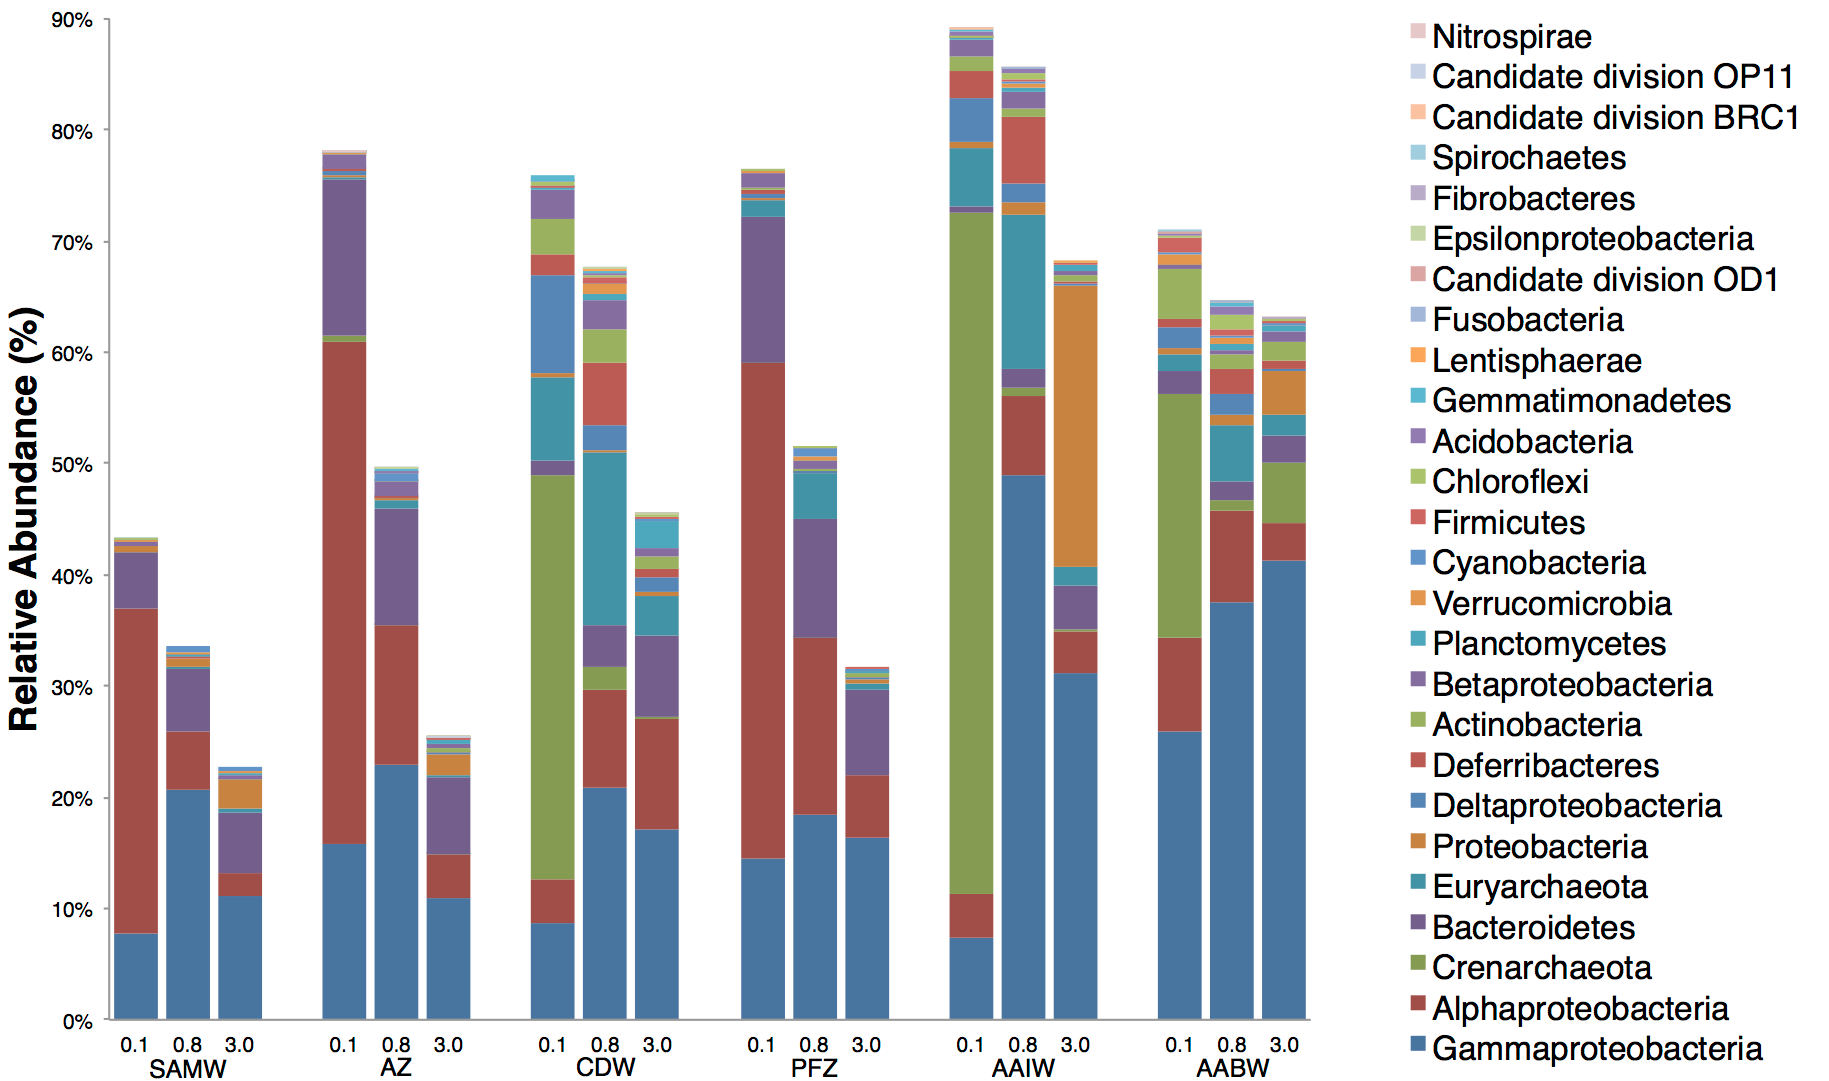
\includegraphics[width=\textwidth]{../advection/taxonomicbarplot.png}
  \caption[OTU assignments in the advection study.]{Taxonomic assignments for each sampled water mass. Water masses (x-axis): Subantarctic Mode Water (SAMW); Antarctic Zone (AZ); Circumpolar Deep Water (CDW); Polar Frontal Zone (PFZ); Antarctic Intermediate Water (AAIW); Antarctic Bottom Water (AABW). Size fractions are given in \micron{}. All \acp{OTU} aggregated to phylum, except for members of the Proteobacteria which were aggregated to class when known. Relative abundance is percentage of all reads assigned to a given taxonomic group and has been scaled to account for unassigned reads.}
  \label{fig:taxonomicbarplot}
\end{figure}


\ac{nMDS} ordination showed that the sampled water masses could be distinguished on the basis of taxonomic distance \figref{fig:nMDStaxonomic}.
This was supported by \ac{ANOSIM} analysis (R = 0.77, p = 0.001).
While each water mass had a distinct taxonomic profile, some broad differences between surface and deep masses were observed \figref{fig:taxonomicbarplot}.
Surface waters (\ac{AZ}, \ac{PFZ}, \ac{SAMW}) were dominated by representatives of the Alphaproteobacteria, Bacteroidetes and Gammaproteobacteria.
The high abundance of Bacteroidetes at the surface reflects their association with phytoplankton, as many species in this lineage specialise in the degradation of high molecular weight products of primary production \cite{Williams:2012gsa}.
Alphaproteobacteria were represented primarily by the SAR11 clade, abundant in ocean surface communities \cite{Morris:2002bn} including the \ac{SO} \cite{Brown:2012gna}, and Roseobacter clades, which have also been associated with degradation of phytoplankton products \cite{Williams:2012gsa, Giebel:2009hr}.
The dominant Gammaproteobacterial orders were the Alteromonadales and Oceanospirillales, typical of \ac{SO} surface waters \cite{Wilkins:2012ii}.
Few archaeal \acp{OTU} were detected, consistent with their well-described decline in abundance during summer \cite{Murray:1998wy, Grzymski:2012ej}.
The deep water masses (\ac{CDW}, \ac{AAIW}, \ac{AABW}) were dominated by Crenarchaeota, Euryarchaeota and Gammaproteobacteria, again consistent with previous findings \cite{LopezGarcia:2001vp}.

\begin{figure}[!ht]
  \centering
  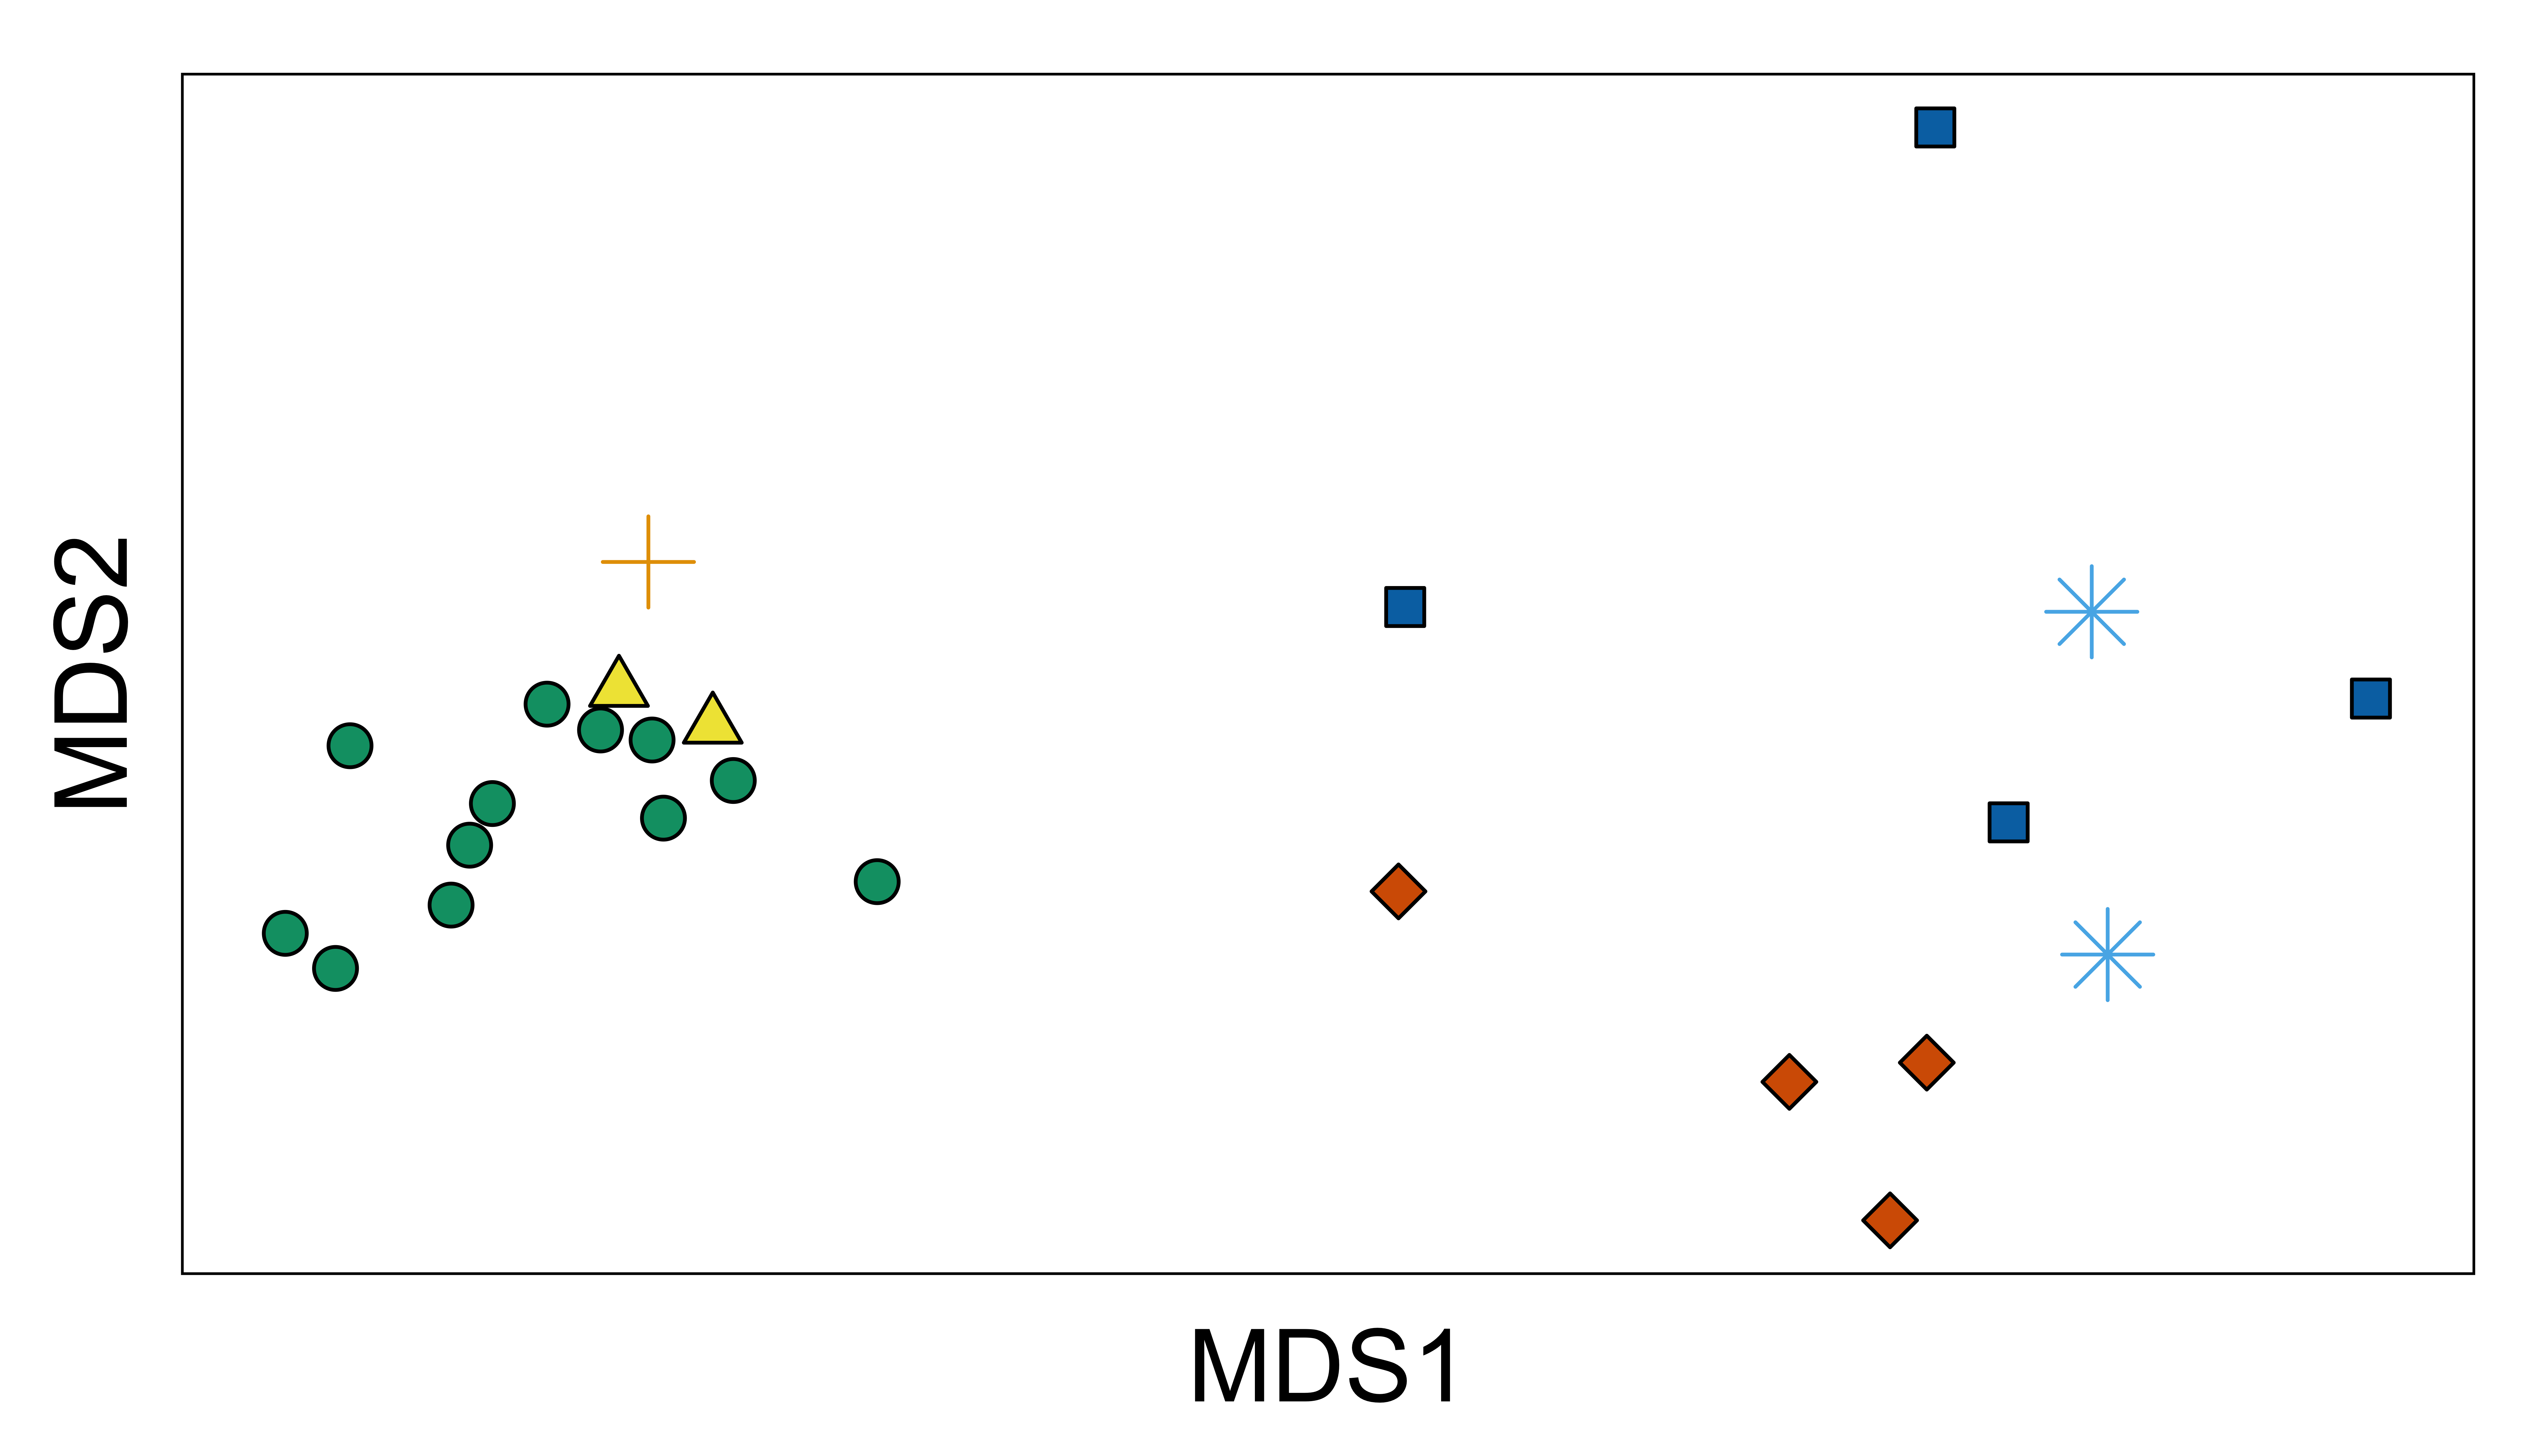
\includegraphics[width=\textwidth]{../advection/nMDStaxonomic.png}
  \caption[nMDS of advective distances between samples.]{nMDS ordination of the taxonomic distance matrix (2D stress = 0.08). Antarctic Intermediate Waters (AAIW), light blue stars; Subantarctic Mode Water (SAMW), orange crosses; Antarctic Bottom Water (AABW), dark blue squares; Antarctic Zone (AZ), green circles; Polar Frontal Zone (PFZ), yellow triangles; Circumpolar Deep Water (CDW), red diamonds.}
  \label{fig:nMDStaxonomic}
\end{figure}


\subsection{Environment and distance effects}
\ac{nMDS} ordination showed that the sampled water masses clustered well on the basis of environmental distance \figref{fig:nMDSenvironmental}.
This was supported by \ac{ANOSIM} (R = 0.84, p = 0.001). 
A partial Mantel test, comparing the taxonomic to environmental matrices with the spatial matrix held constant, found a correlation of r = 0.48 (p = 0.001), indicating a strong environment effect.

\begin{figure}[!ht]
  \centering
  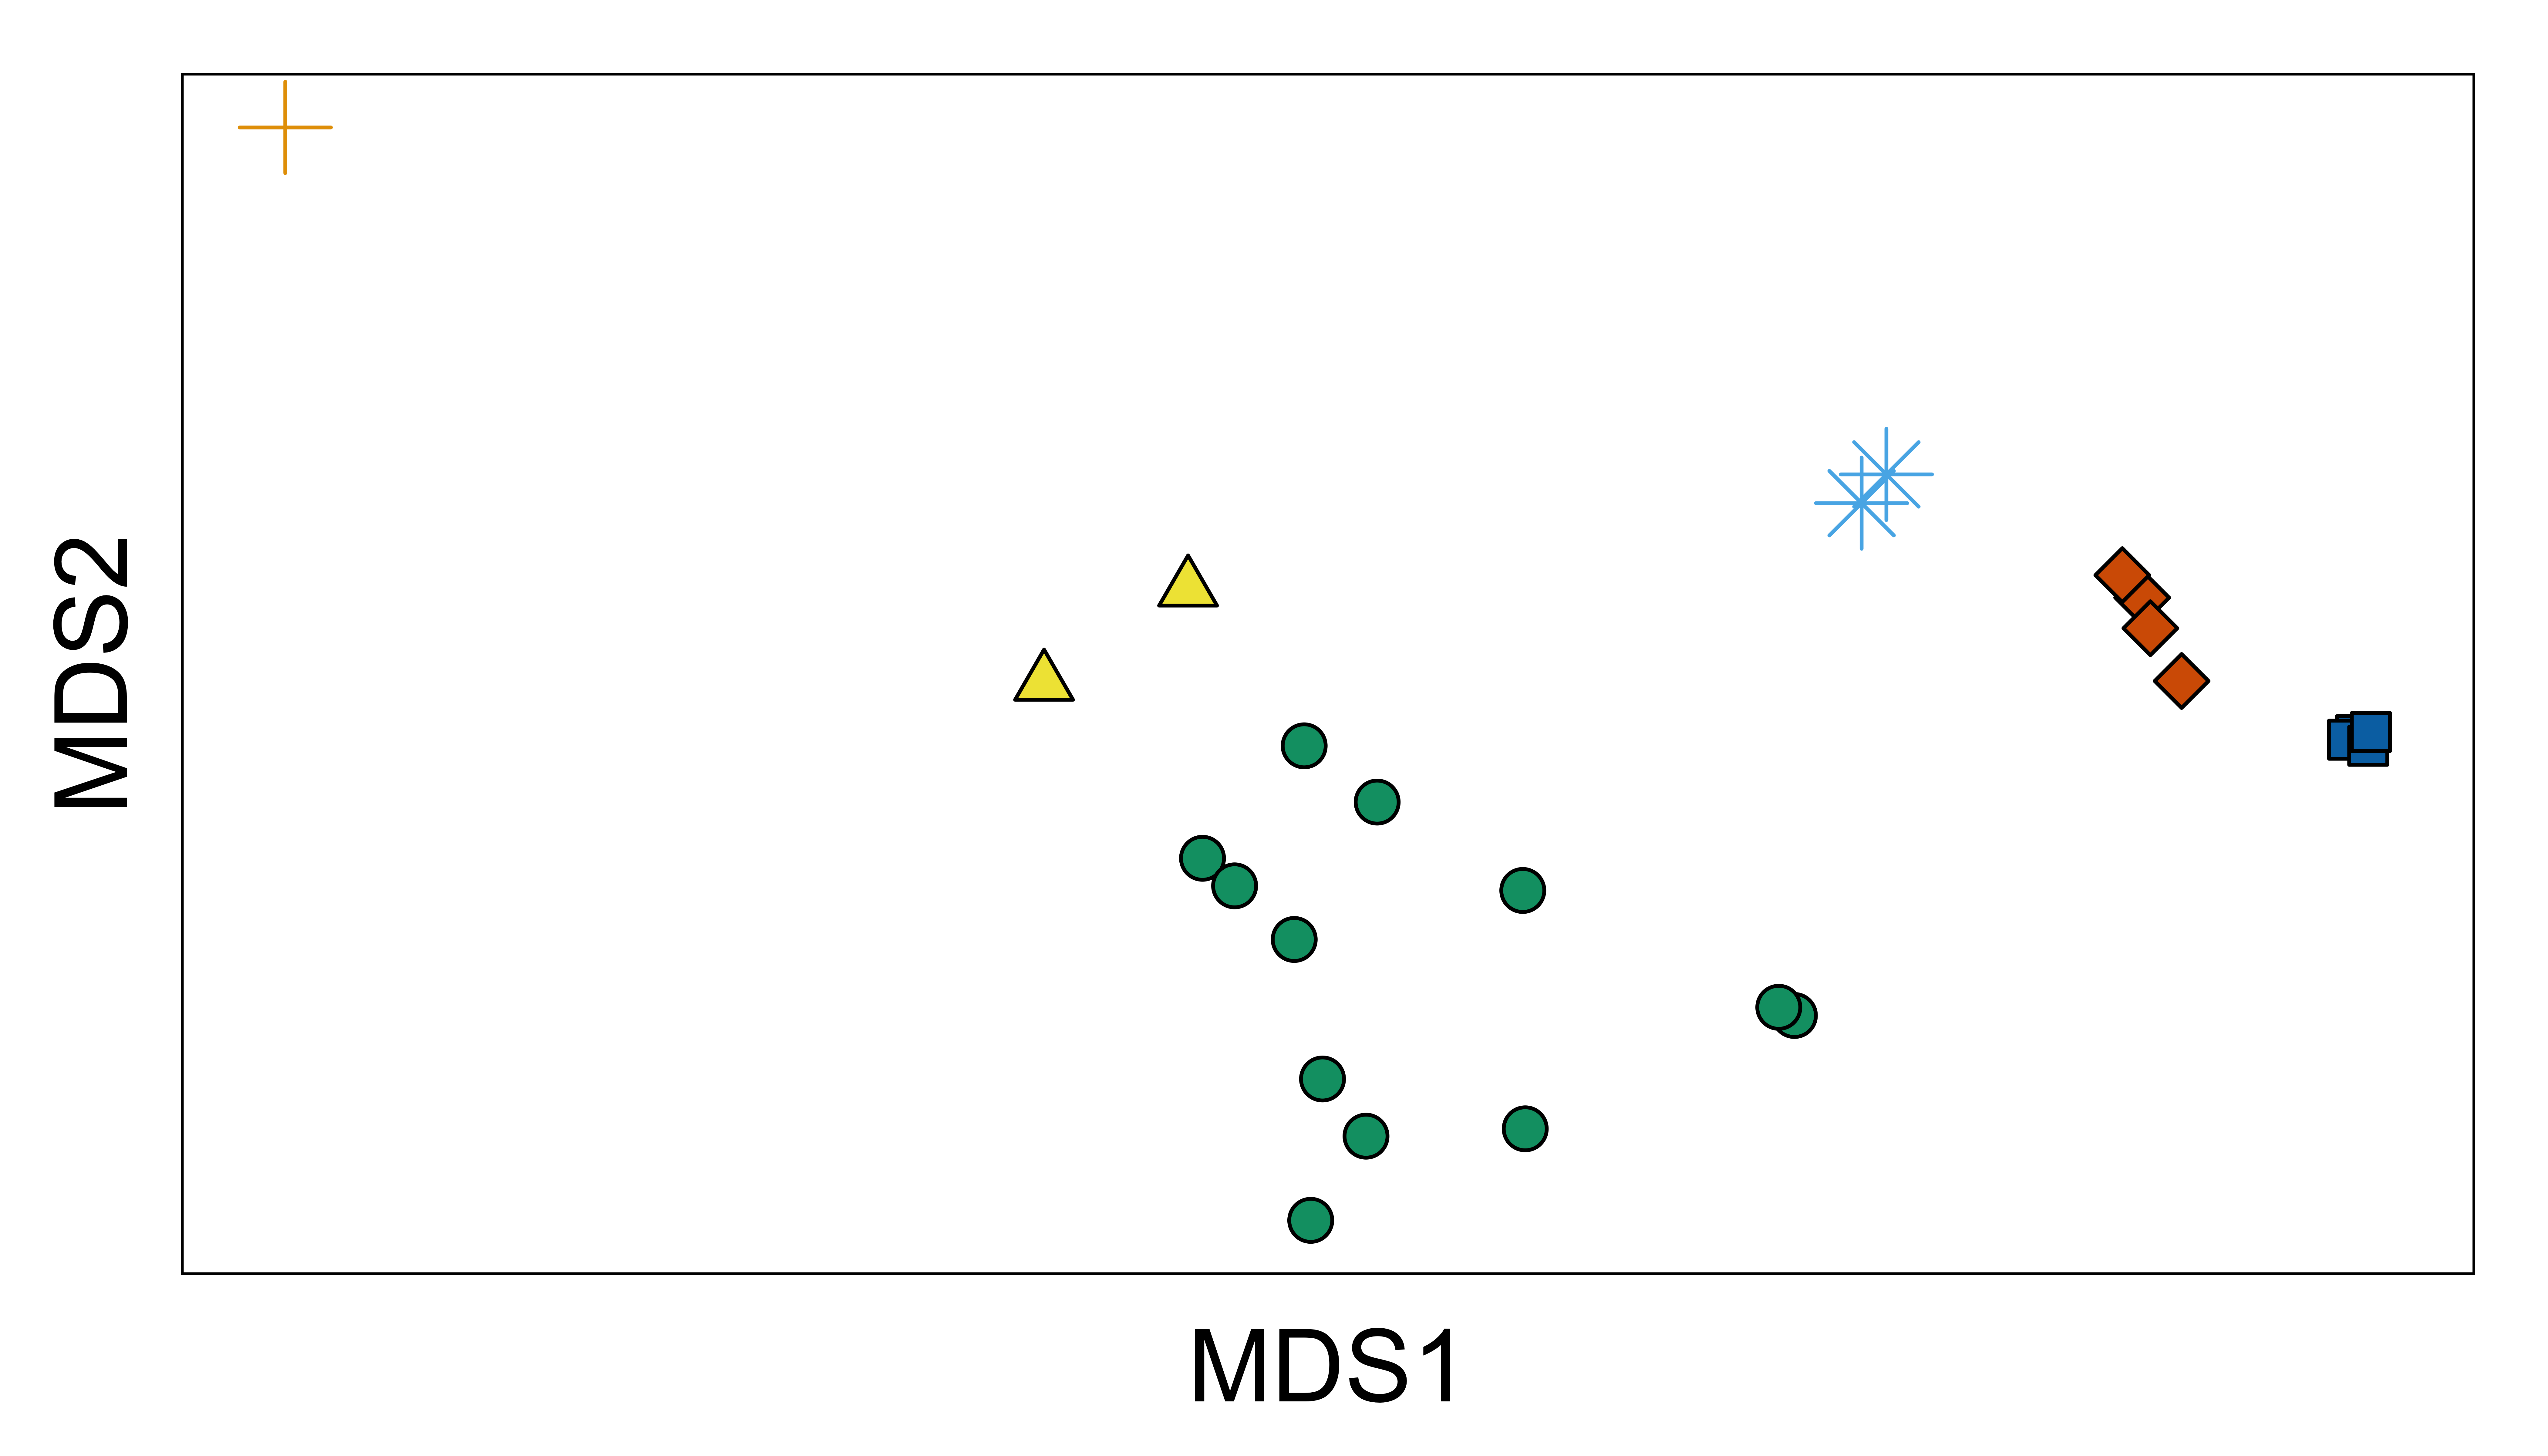
\includegraphics[width=\textwidth]{../advection/nMDSenvironmental.png}
  \caption[nMDS of advective distances between samples.]{nMDS ordination of the environmental distance matrix (2D stress = 0.02). Antarctic Intermediate Waters (AAIW), light blue stars; Subantarctic Mode Water (SAMW), orange crosses; Antarctic Bottom Water (AABW), dark blue squares; Antarctic Zone (AZ), green circles; Polar Frontal Zone (PFZ), yellow triangles; Circumpolar Deep Water (CDW), red diamonds.}
  \label{fig:nMDSenvironmental}
\end{figure}


\ac{distLM} analysis of the individual physicochemical variables found that considered separately, each of phosphate, silicate, nitrate, oxygen, salinity and pressure explained 17--35\% of the taxonomic variance between samples (p = 0.001).
Temperature had no significant effect on taxonomic composition when considered separately (p \textgreater{} 0.05).
When all combinations of variables were considered (BEST modelling), the best model consisted of all variables with the exception of phosphate (adjusted R\textsuperscript{2} = 0.44), with the full set of variables only marginally worse (adjusted R\textsuperscript{2} = 0.43).
The rejection of phosphate may reflect a redundancy in the measurement of both phosphate and nitrate; these are often held to be constant throughout the ocean at the Redfield ratio of N:P \textapprox{}16:1 \cite{Anderson:1994vb}.
However, deviation from this ratio has been observed in the \ac{SO} and related to iron concentration (which was not measured in this study) and to phytoplankton abundance \cite{Weber:2010fi}.
For these reasons, and because of the marginal effect of discarding phosphate from the variable selection, it was retained when generating the environmental distance matrix.

The \ac{dbRDA} plot showed the six variables retained by the \ac{distLM} model (i.e.\ all except phosphate) structured the samples first along an axis separating surface and deep samples (dbRDA1), strongly related to dissolved oxygen (r = 0.79) \figref{fig:dbRDA}.
The second axis was best correlated with temperature (r = \textminus{}0.75).
All six retained variables had a moderate correlation with at least one of the first two axes \tabref{tab:dbRDAcorrs}.
As with the \ac{nMDS} ordinations \figref{fig:nMDStaxonomic,fig:nMDSenvironmental,fig:nMDSadvection}, the water masses were generally well separated by the first two \ac{dbRDA} axes.
Samples from the \ac{AABW} and \ac{AAIW}, which were not separated by the first two axes, were clearly separated along the third \tabref{tab:dbRDAcorrs}, which was best correlated with pressure (r = \textminus{}0.79).
This suggests that these two masses had similar physicochemical properties, and were mainly distinguished by depth, consistent with their common origin in sinking Antarctic Surface Waters \cite{Foldvik:1988gp}.

\begin{figure}[!ht]
  \centering
  \includegraphics[width=\textwidth]{../advection/dbRDA.png}
  \caption[dbRDA ordination of relationship between environment and community.]{dbRDA ordination of the distLM model describing the relationship between the BEST-selected set of predictor physicochemical variables (pressure, oxygen, temperature, salinity, silicate, and nitrate) and the taxonomic dissimilarity between samples. Vectors represent the effect of each predictor variable on the two visualised axes. Vector length corresponds to the relative size of the effect, while direction represents the correlations to the two displayed axes. The first axis (dbRDA1) captures 64\% of fitted and 37\% of total variation between the samples' taxonomic profiles; the second (dbRDA2) captures 14\% of fitted and 8\% of total variation. Antarctic Intermediate Waters (AAIW), light blue stars; Subantarctic Mode Water (SAMW), orange crosses; Antarctic Bottom Water (AABW), dark blue squares; Antarctic Zone (AZ), green circles; Polar Frontal Zone (PFZ), yellow triangles; Circumpolar Deep Water (CDW), red diamonds.}
  \label{fig:dbRDA}
\end{figure}

\begin{table}[!ht]
\centering
\sffamily
\caption[Correlations between dbRDA axes and physicochemical variables]{Correlations between dbRDA coordinate axes and physicochemical variables (multiple partial correlations).}
\label{tab:dbRDAcorrs}
\begin{tabular}{lllllll}
\toprule
\textbf{Variable} & \textbf{dbRDA1} & \textbf{dbRDA2} & \textbf{dbRDA3} & \textbf{dbRDA4} & \textbf{dbRDA5} & \textbf{dbRDA6}\\
\midrule
Pressure & \textminus{}0.316 & \textminus{}0.485 & \textminus{}0.787 & \textminus{}0.148 & \textminus{}0.144 & \textminus{}0.048\\
Oxygen & 0.792 & \textminus{}0.171 & \textminus{}0.125 & 0.069 & \textminus{}0.567 & 0.050\\
Temperature & \textminus{}0.025 & \textminus{}0.750 & 0.366 & 0.236 & 0.180 & 0.463\\
Nitrate & \textminus{}0.311 & 0.007 & 0.325 & \textminus{}0.636 & \textminus{}0.561 & 0.281\\
Silicate & \textminus{}0.303 & 0.341 & \textminus{}0.166 & 0.615 & \textminus{}0.371 & 0.498\\
Salinity & \textminus{}0.290 & \textminus{}0.239 & 0.311 & 0.368 & \textminus{}0.417 & \textminus{}0.673\\
\bottomrule
\end{tabular}
\end{table}


A distance effect was detected by comparing the taxonomic and spatial matrices with the environmental matrix held constant (partial Mantel; r = 0.38, p = 0.003).
This indicated that a process other than contemporary environmental selection was appreciably affecting variation in microbial community composition.

\subsection{Testing the advection effect}

244,000 encounters were recorded between particles and sample sites during the 100 year advection simulation.
Encounter times spanned the full range of the simulation (5 days--100 years), with a median of 30 days and mean of 3018 days.
47 pairs of samples did not yield mutual encounters (i.e.\ at least one particle from one sample encountering the other).
Of these, every pair included at least one AABW sample.

\ac{nMDS} ordination showed that the sampled water masses could be broadly distinguished on the basis of their mutual advection distances \figref{fig:nMDSadvection}.
This was supported by \ac{ANOSIM} (R = 0.41, p = 0.002).

\begin{figure}[!ht]
  \centering
  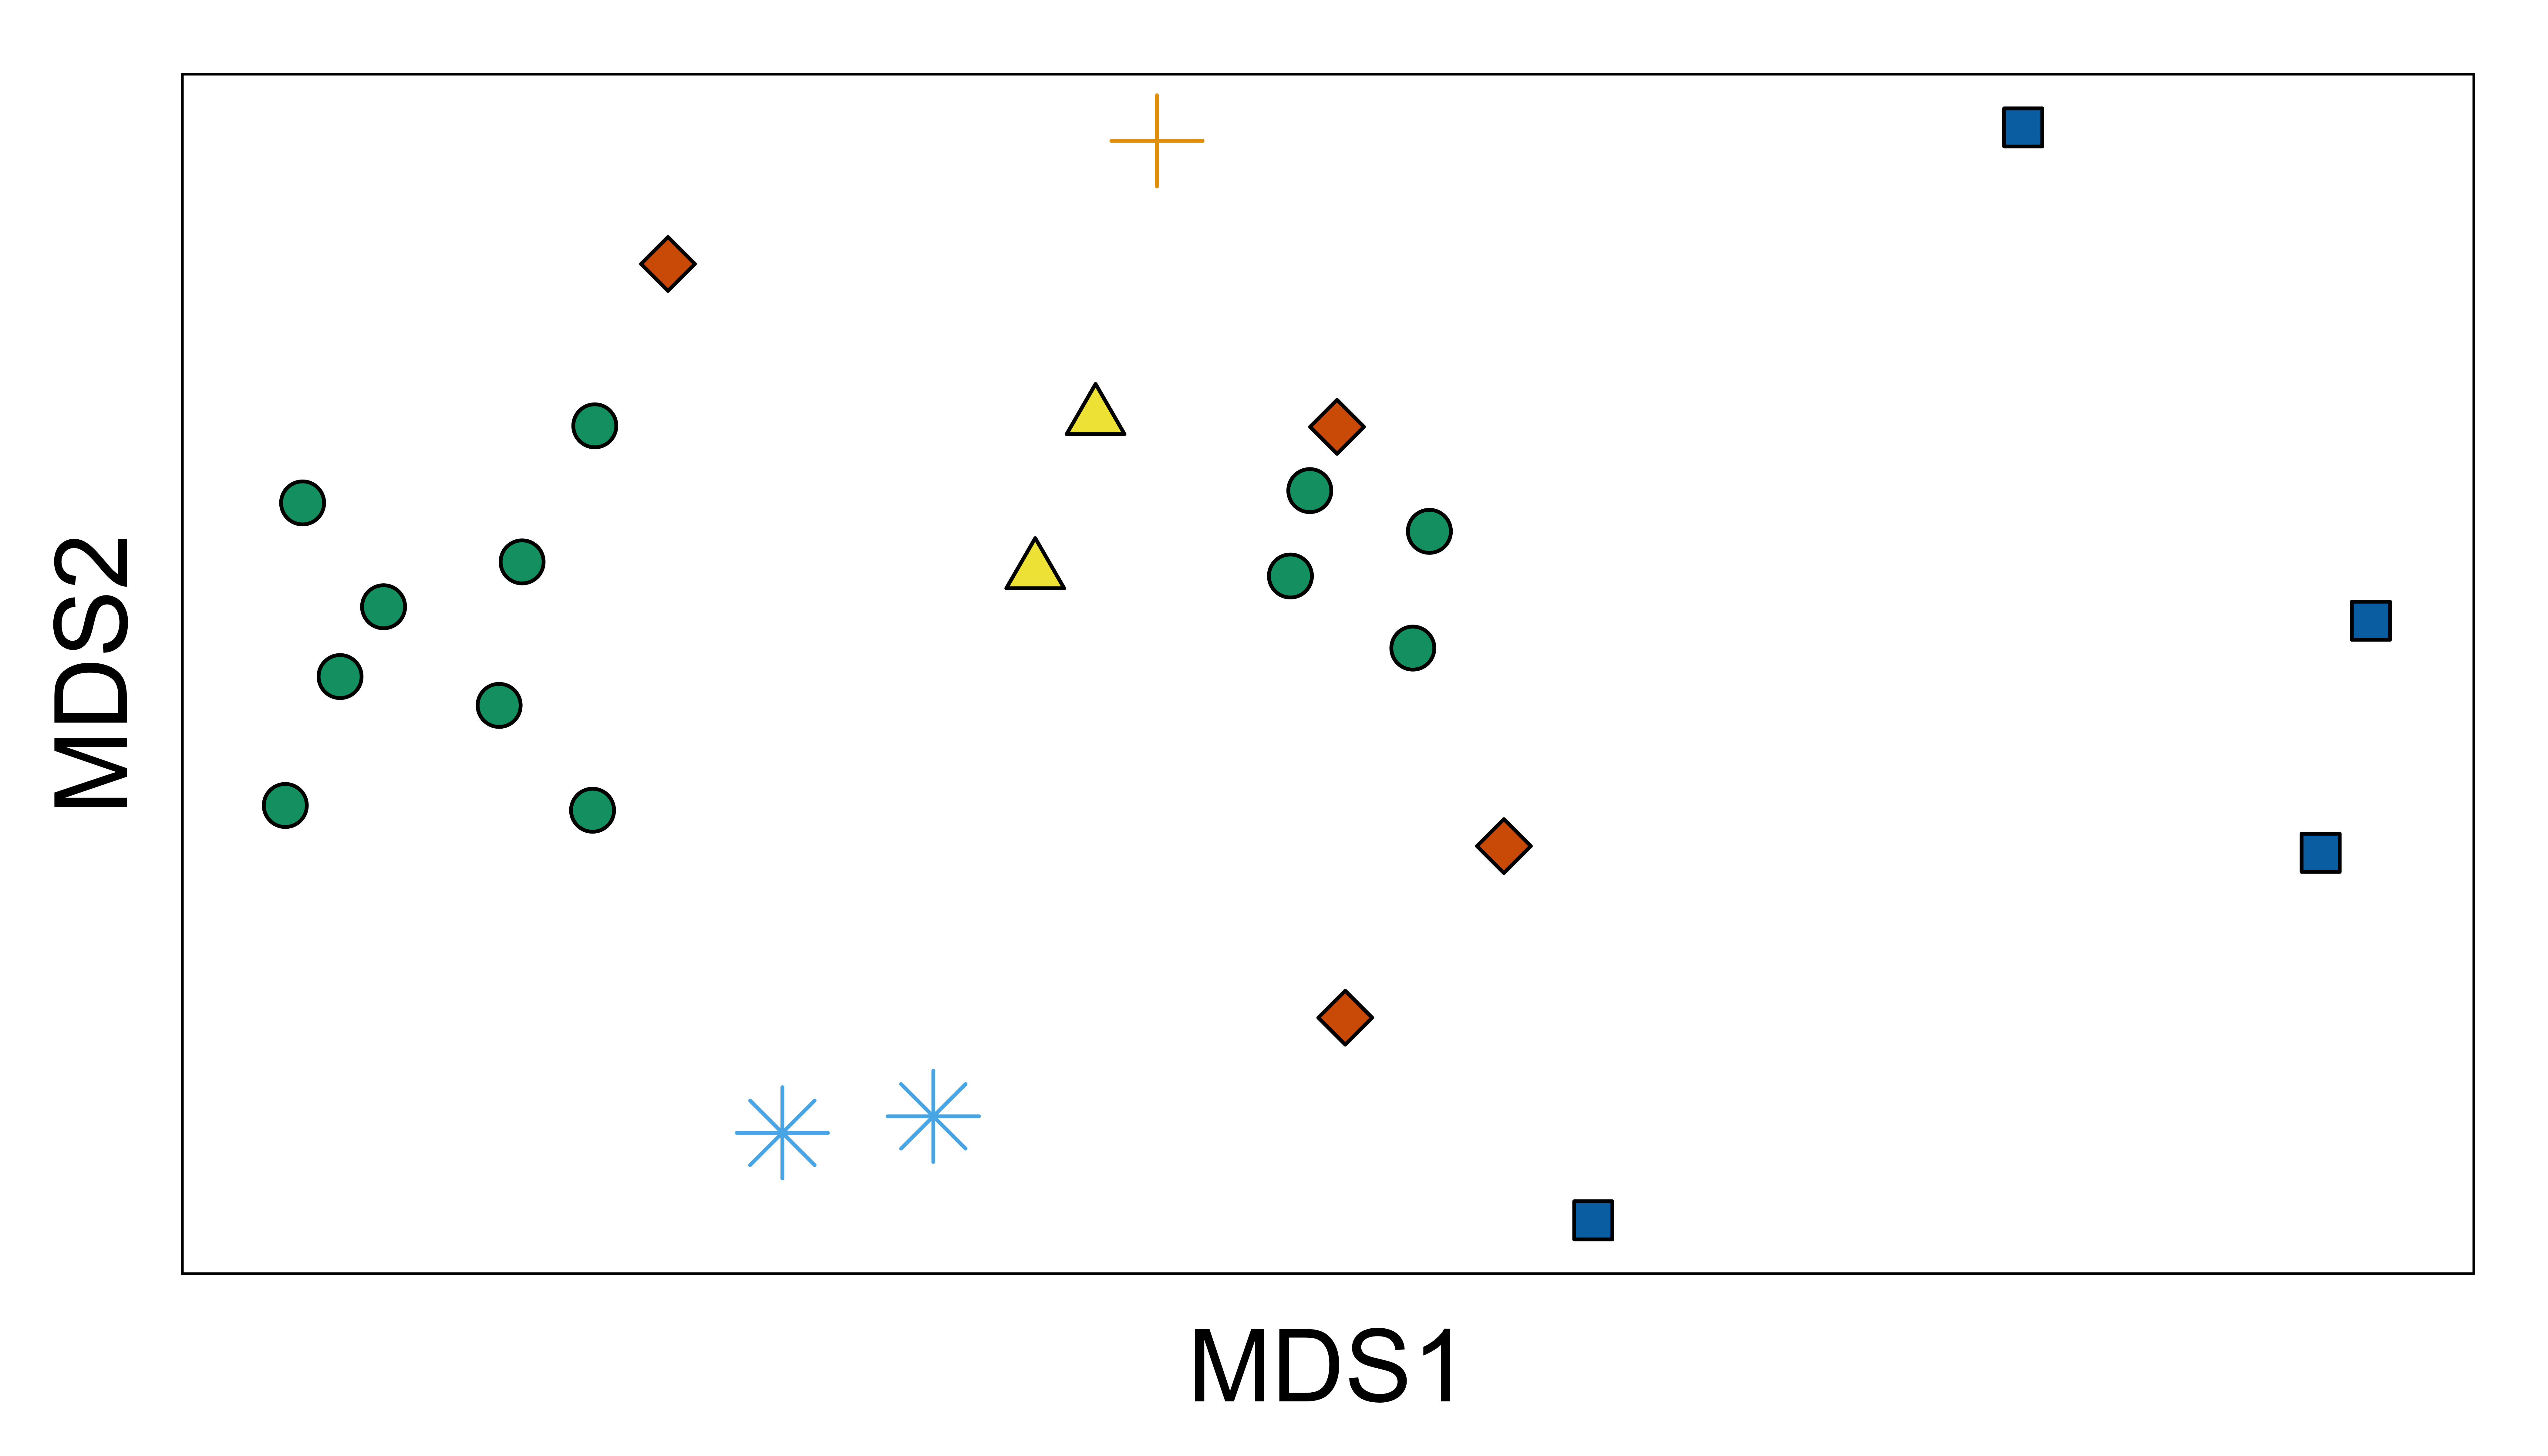
\includegraphics[width=\textwidth]{../advection/nMDSadvection.png}
  \caption[nMDS of advective distances between samples.]{nMDS ordination of the advection distance matrix (2D stress = 0.19). Antarctic Intermediate Waters (AAIW), light blue stars; Subantarctic Mode Water (SAMW), orange crosses; Antarctic Bottom Water (AABW), dark blue squares; Antarctic Zone (AZ), green circles; Polar Frontal Zone (PFZ), yellow triangles; Circumpolar Deep Water (CDW), red diamonds.}
  \label{fig:nMDSadvection}
\end{figure}


A partial Mantel test, comparing the taxonomic and advection matrices with the spatial and environmental matrices held constant, showed that advection has a moderate (r = 0.28) and significant (p = 0.010) correlation with taxonomic composition independent of spatial and environmental factors.
To ensure this result was not unduly influenced by the samples on which the 100 year ceiling was imposed (\ac{AABW}) and those for which particle releases were not simulated (samples 11, 13, 17 and 22), the test was repeated with these samples removed.
The correlation was stronger and remained significant despite the smaller sample size (r = 0.36, p = 0.025).
To ensure the result was robust to the choice of advection distance metric, correlations were recalculated for both the full set of samples and the subset (excluding \ac{AABW} and samples 11, 13, 17 and 22) with pairwise advection distance defined as the mean time for all particle encounters between samples.
The observed correlation was higher using this metric for both the full set (r = 0.40, p = 0.0090) and subset (r = 0.52, p = 0.0070).
\softwarename{SourceTracker} analysis confirmed that the effect was moderately directional, with the proportion of \acp{OTU} contributed from a given ``source'' sample to a ``sink'' sample correlated with the proportion of particle encounters it generates (Spearman's \textrho{} = 0.15, p = 0.0015). 

To explore the role of taxonomic resolution in the detection of an advection effect, partial Mantel tests were repeated as above with \acp{OTU} aggregated to each of the seven standard taxonomic ranks.
Aggregation to genus resulted in a higher correlation (r = 0.29, p = 0.02) than to species, but with this exception a pattern of decreasing correlation with coarser rank was observed \figref{fig:taxonomicresolution}.

\begin{figure}[!ht]
  \centering
  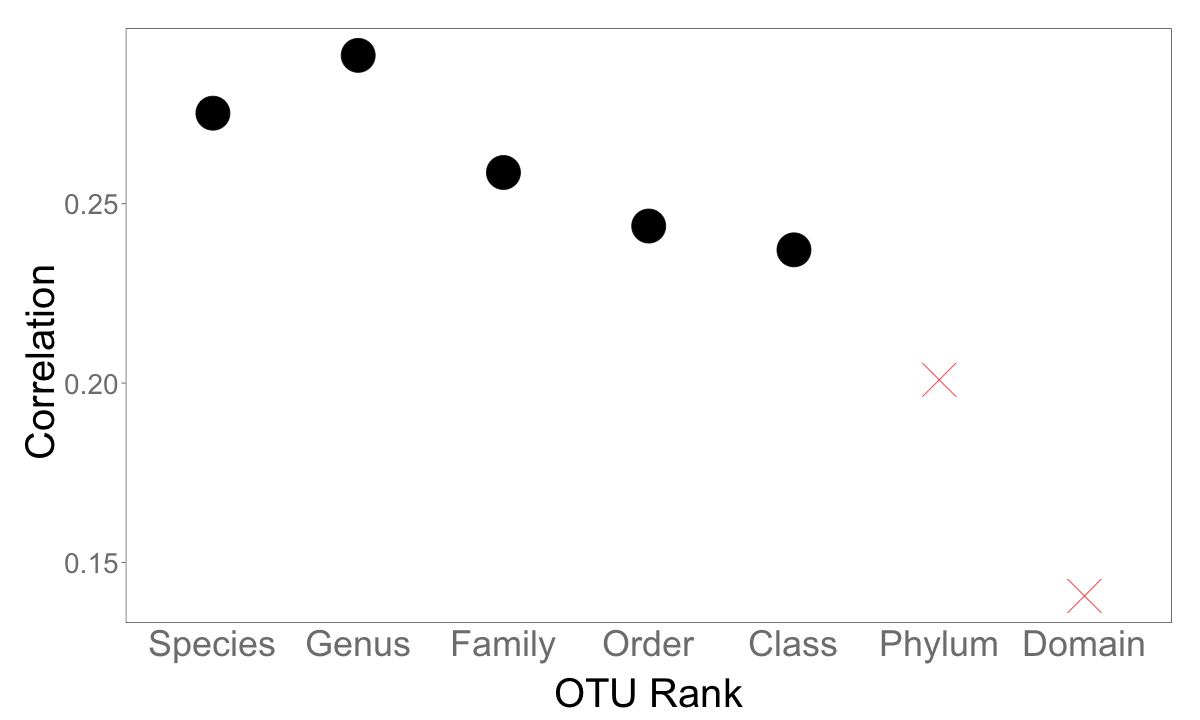
\includegraphics[width=\textwidth]{../advection/taxonomicresolution.png}
  \caption[Advection effect at different taxonomic resolutions]{Effect of taxonomic resolution on partial Mantel correlation between advection and taxonomic distances, with environmental and spatial distances held constant.
  Significant correlations (right-tailed p-value after 999 random permutations \textgreater{} 0.05), black circles; not significant correlations (\textlessthanorequal{} 0.05), red crosses.}
  \label{fig:taxonomicresolution}
\end{figure}


\subsection{Testing advection effect mechanisms}

Two explanations can be proposed for the relationship between advection and community composition.
The first is that advection increases microbial dispersal by increasing the probability that \acp{OTU} from one site will encounter and colonise another (the ``dispersal mechanism'').
This assumes microbial dispersal is less than perfect; i.e.\ that ``everything is not everywhere''.
The second is that advection transports a large numbers of cells at a rate measurably outpacing environmental selection, regardless of whether or not those cells are able to successfully colonise (i.e.\ grow and reproduce in) downstream sites: that ``the environment selects, but not fast enough'' (the ``bulk transport mechanism'').
Considering the long advection times between sites in this study, the relatively rapid growth of marine microorganisms, and the ability of small numbers of cells to rapidly reduce \textbeta{}-diversity between isolated marine sites \cite{Declerck:2013cz}, the dispersal mechanism seems the more plausible.

Two tests were performed to distinguish between these hypotheses.
Firstly, the advection distance matrix was reconstructed using the absolute pairwise number of particle encounters as the distance metric between samples (distance metric for given sample pair = maximum number of encounters across all sample pairs \textminus{} encounters for given pair + 1).
There was no significant correlation between this matrix and the taxonomic distance matrix when the environmental and spatial matrices were held constant (p \textgreater{} 0.05).
This suggests that advection time, not the absolute number of transported cells, is the relevant factor, supporting the dispersal mechanism.

Secondly, it was reasoned that under the dispersal mechanism, advection would have a large effect on the presence and diversity of taxa and a smaller effect on their abundances; while if the bulk transport hypothesis held, the effect would largely be on the relative abundances.
To test this, the taxonomic profiles were transformed to a presence/absence measure (\ac{OTU} present = 1, absent = 0), and a matrix of S\o{}rensen dissimilarities generated.
The advection effect was stronger (r = 0.33, p = 0.004) than when abundances were considered, again supporting the dispersal hypothesis. 

\section{Discussion}

This study found good support for the hypothesis that advection shapes microbial assemblages independent of an environment or distance effect.
Communities that are more closely connected by advection are more similar, and this effect exists even when environment and distance effects are controlled for.
The results also indicate that advection primarily shapes microbial community structure by increasing opportunities for colonisation, rather than transporting large numbers of cells to downstream sites. 

The major alternative hypothesis for the observed correlation is that there exists an unmeasured environmental variable (e.g.\ iron concentration, pH) which correlates well with both advection and community composition.
As in all studies of historical influences on microbial biogeography, it is impossible to eliminate all potential confounding variables.
However, a rigourous confirmation of the advection effect will require future work to measure physicochemical paramaters as comprehensively as possible.

The amount of variance in taxonomic composition explained by the advection effect can be estimated as the square of the correlation coefficient (r\textsuperscript{2}).
This value, 7\%, is likely to be a conservative estimate, as this study only captured advective pathways from one sample to another; it is possible that some samples with a large mutual advective distance shared a common advective source outside the study area.
A recent review of studies partitioning variance in microbial community composition found that the mean reported variance explained by a distance effect was 10\%, and by an environment effect 27\% \cite{Hanson:2012cb}.
The estimated proportions of variance in this study, 14\% (p = 0.001) for distance and 23\% (p = 0.001) for environment, were close to these values.
While there are no comparative data for the advection effect in other systems, the value of at least 7\% for the \ac{SO} indicates that advection is important relative to both distance and environment effects. 

Taxonomic resolution (i.e.\ the level of genetic difference at which \acp{OTU} are discriminated) often determines whether or not a pattern is detected in studies of microbial distance effects, with finer resolutions generally leading to an increased likelihood of detecting a significant effect \cite{Hanson:2012cb}.
Surprisingly, aggregation to genus resulted in a higher correlation than to species \figref{fig:taxonomicresolution}.
This may be because of the selection of the V6--V8 hypervariable regions as the sequencing target.
Amplification of the V6 region alone has been shown to underestimate species richness, while targeting the V7--V8 region overestimates it \cite{Youssef:2009un}.
It is possible that due to this choice of target, the ``species''-level aggregation represents a much finer taxonomic resolution at which intra-species variability begins to overwhelm the advection effect.
With this exception, the pattern of a decreasing effect with coarser taxonomic resolution was confirmed, with no statistically significant effect for aggregation to phylum or domain.

\subsection{Future work}

To obtain a better understanding of the advection effect, it would be useful to determine whether particular taxonomic or physiological groups are more amenable to dispersal by advection; e.g.\ through the formation of dormant spores \cite{Sul:2013in, Bissett:2010wj}.
As it is possible that an unmeasured environmental variable (e.g.\ iron concentration, see Discussion) also correlates with both advection and community composition, future studies should address this.
Finally, further mesocosm experiments like those reported by \citet{Declerck:2013cz} will be useful to confirm the effect of small-scale exchange of cells between sites on colonisation and community structure.


%reset acronyms
\glsresetall
\chapter{General discussion}
\label{ch:generaldiscussion}

\section{Contributions of this thesis}

This thesis aimed to investigate the microbial ecology and biogeography of the \ac{SO}.
To achieve this, two factors that structure the biogeographic distribution of microorganisms in the \ac{SO} were selected for study: the \ac{PF}, a major biogeographic barrier, and advection, a potentially major biogeographic force.

\subsection{The Polar Front}

This project found good evidence that the \ac{PF} is a major biogeographic barrier in the \ac{SO}, by demonstrating that the bacterial and archaeal communities in the waters to the south (the \ac{AZ}) are significantly different from the waters to the north (the \ac{SAZ} and subtropical waters north of the \ac{STF}, primarily representing \ac{SAMW}) (\secreft{ch:polarfront}).

This is not the first study on the effect of the \ac{PF} on the distribution of \ac{SO} microbiota.
Variation in the position of the \ac{ACC}, which determines the location of the \ac{PF}, has been shown to influence zooplankton composition \citep[e.g.][]{Chiba:2001un,Hunt:2001vp}, including dinoflagellates \cite{Esper:2002ui}\footnote{Interestingly, one study described the biogeographic effect of \ac{ACC}-associated fronts on zooplankton as being only weakly related to environmental parameters \cite{Ward:2003db}, suggesting the effect of advection (\secreft{ch:advection}) on zooplankton as a potential avenue for future research}.
The \ac{ACC} and/or \ac{PF} have similarly been shown to influence the distribution of Roseobacter phylotypes \cite{Selje:2004ka,Giebel:2009hr}, Flavobacteria \cite{Abell:2005ji}, and SAR11 phylotypes \cite{Giebel:2009hr}.
However, this thesis provides a significant contribution, presenting the first community-level (metagenomic) survey of \ac{SO} bacterial and archaeal plankton performed over a latitudinal transect occupying all major \ac{SO} surface water masses to give an integrated snapshot of the microbial ecology and biogeography of the \ac{SO}.

As well as the confirming previous findings on the level of individual taxonomic groups, this study found that the effect of the \ac{PF} extends to the whole community, and even to the distribution of genomically encoded functional potential.
The higher abundance south of the \ac{PF} of Bacteroidetes and Rhodobacterales, associated with the degradation of phytoplanktonic byproducts \citep[e.g.][]{Buchan:2005hd,Williams:2012gsa}, reflect the higher concentrations of (primarily eukaryotic) phytoplankton in this region. 
This was also reflected in the functional analysis, with an overrepresentation of high-specificity transporters, suggestive of copiotrophic taxa in a ``feast'' phase \cite{Lauro:2009gx}.
In general, waters south of the \ac{PF} reflected the upwelling of nutrient-rich \ac{NADW} and higher supply of light during the austral summer, which make the region significantly more active and productive than \ac{SAZ} and even subtropical waters to the north.

These northern waters were characterised by a higher relative abundance of slow-growing, nutrient-scavenging oligotrophs such as SAR11 and SAR116.
Functionally, this was reflected in the higher abundance of genes encoding branched-chain amino acid transporters, which both SAR11 and SAR116 possess.
The other significant feature of region north of the \ac{PF} was the higher abundance of the cyanobacterial genera \genus{Prochlorococcus} and \genus{Synechococcus}, and concurrently the photosynthesis functions they encode.
This was most likely due to the sensitivity of these genera to temperature.

\subsubsection{Biogeographic role of the Polar Front}

Having shown that the \ac{PF} is a major biogeographic barrier, and in light of the advection study also presented in this thesis (\secreft{ch:advection}), it is worth considering the mechanism(s) by which the \ac{PF} shapes microbial biogeography.
It is likely that three main forces are at work.

The first is the role of the \ac{PF} as a ``biogeographic barrier'' in the classical sense in which the term is applied to macroorganisms.
In other words, it physically prevents or slows the migration of cells between the regions it divides, leading if not to allopatric speciation, at least to some degree of genetic divergence, which is amplified by the differences in environmental properties.
\citet{Selje:2004ka}, who first reported that \ac{RCA} phylotypes differed across the \ac{PF}, offered this mechanism as a likely explanation, an idea corroborated by further reports on RCA \cite{Giebel:2009hr} and Flavobacteria \cite{Abell:2005ji}.
The advection effect (\secreft{ch:advection}) supports such a mechanism, by showing that oceanic regions poorly connected by advection (i.e.\ poorly mixed) have less similar microbial communities.

The second mechanism, complementary to the first, is the difference in physicochemical properties resulting from the same oceanographic forces that create the \ac{PF}: in particular, the advective distribution of nutrients.
The ratio of biological N/P export in \ac{SO} surface waters increases northwards from the region of upwelling \ac{CDW} in the \ac{AZ} (N/P\textsubscript{exp} \textless{} 16) to the \ac{SAZ} (N/P\textsubscript{exp} \textgreater{} 16) \cite{Weber:2010fi}.
This directly contradicts the standard assumption that \ce{PO4^3-} is exported to the deep ocean in a fixed proportion of \textapprox{}16:1 available \ce{NO3^-} to \ce{PO4^3-} (the Redfield ratio).
\citet{Weber:2010fi} convincingly showed that this is largely a result of the biogeographic distribution of low cellular N/P diatoms relative to other high cellular N/P plankton.
The distribution of diatoms in the \ac{SO} is in turn controlled by the concentration of silicic acid \cite{MFranck:2000kt}, which supplied in abundance south of the \ac{PF} by upwelling \ac{CDW} but is limiting further north \citep[widely held, but well summarised by][]{Coale:2004to}, explaining the observed difference in N/P\textsubscript{exp}.
Further, \citet{Weber:2010fi} showed that advective mixing of organic N and P exported to the deep ocean by sinking organic matter and remineralised in the aphotic zone was sufficient to counterbalance the differential export of N and P by diatoms and other plankton, leading to an equilibrium approximately equivalent to the Redfield ratio of 16:1 N:P.
Advective transport of nutrients and the distribution of plankton are thus intimately connected in the \ac{SO}, with the \ac{PF} acting as a key barrier between the nutrient-rich \ac{AZ} upwelling and the comparatively oligotrophic \ac{SAZ}.
As well as the distribution of these major nutrients (N, P and Si), the waters to the north and south of the \ac{PF} differ in temperature and salinity due to their different circulatory origins \cite{Foldvik:1988gp}.

The third mechanism by which the \ac{PF} may act as a biogeographic boundary is more mundane.
Being a polar ocean, the \ac{SO} is subject to strong latitudinal gradients in air temperature and sunlight unrelated to its oceanographic structure.
The Antarctic Circle, the latitude at which continuous 24-hour periods of sunlight (and of darkness) become possible, is considerably south of the \ac{PF} (\textapprox{}66.5\textdegree{} S, although this varies due to slow changes in the Earth's axial tilt).
However, the existence of large environmental gradients means that longitudinal features (fronts, currents, divergences and convergences in both the ocean and atmosphere) are almost certain to be associated with biological discontinuities simply by virtue of lying on a particular latitude, without necessarily having any causal relationship.
It is likely that latitudinal gradients not directly related to the \ac{PF} (particularly sunlight) make some contribution to the biogeographic pattern.

\subsubsection{The Polar Front and climate change}

Global climate change is already having a large effect on the \ac{SO}.
The \ac{ACC} is largely driven by the strong westerly winds that are characteristic of sub-polar Ferrel cells in atmospheric circulation.
The \ac{SAM} (also known as the Antarctic Oscillation) is a complex, low-frequency oscillation in the latitude and speed of this westerly wind belt between ``positive'' (further south, stronger flow) and ''negative'' (further north, weaker flow) phases.
As a result of climate change, the long-term trend of the \ac{SAM} may be towards the positive phase \cite{Thompson:2002ic}.
Along with an increase in the temperature of \ac{ACC} waters (also due to climate change \cite{Aoki:2003fo,Boning:2008il}), this may be responsible for the observed southward migration of the mean position of the \ac{ACC} by \textapprox{}50 km since the 1950s \cite{Gille:2002fr}.
Even with optimistic assumptions about future anthropogenic greenhouse gas emissions, it has been predicted to move a further \textapprox{}1.4\textdegree{} south (\textapprox{}150 km) by the year 2100 \cite{Fyfe:2005vp}.

The effects of climate change on marine ecology are often thought of in terms of changes in physicochemical properties such as temperature, salinity, pH, and atmospheric \ce{CO_{2}}.
However, changes to the location of biogeographic barriers such as the \ac{PF} may also be significant.
Southward migration of the \ac{PF} will displace a large surface area of \ac{AZ} waters enriched by upwelling nutrients, increasing the relative area of the comparatively oligotrophic \ac{SAZ}.
This may result in a net decrease in primary production, although concurrent changes in temperature and other physicochemical properties make this difficult to predict.
As the \ac{SO} is a major site for sequestration of anthropogenic \ce{CO_2} through the biological pump \cite{Thomalla:2011hi}, this raises the possibility of creating a negative feedback loop \cite{Cox:2000ko} which would further accelerate global climate change.

\subsubsection{Future work}

One of the limitations of the \ac{PF} study was the latitudinal coverage provided by the sample sites.
While this was sufficient to investigate the biogeographic role of the \ac{PF}, it was not fine-scaled enough to conclusively resolve the effects of other fronts.
Moreover, the study only examined surface waters.
A large-scale gridded (latitude, longitude and depth) survey would be of enormous value in linking \ac{SO} microbial communities to their oceanographic context.
Regular samples from the same stations over an annual cycle would also be useful in establishing seasonal changes.

The expense and logistical difficulty of sampling in the \ac{SO}, especially in higher latitudes and during winter months, are a major challenge for future metagenomic surveys.
Current progress on autonomous \textit{in situ} microbial sampling and analysis instruments \cite{CSIRO:2012uw} has the potential to reduce these limitations and provide a robust platform for future work.
These platforms aim to replicate the enormous success of the global Argo network of autonomous oceanographic floats, by combining instrumentation for simple abiotic measurements with the automatic filter collection and storage of seawater biomass for later retrieval and metagenomic analysis.
\textit{In situ} community analysis, for example with onboard microfluidics and a DNA microarray system such as PhyloChip (Berkeley Lab, Berkeley, USA) are also under consideration \cite{CSIRO:2012uw}.
A network of even a small number of these probes could quickly exceed shipboard sampling efforts at a lower cost, and provide better coverage of logistically difficult regions and times of year in the \ac{SO}.

An advantage of the shotgun metagenomic approach as employed in the \ac{PF} study is the ability to identify the functional potential of sampled microorganisms, as revealed by their encoded genes.
However, genomic potential is only a window into the actual ecological function of microbes: it does not take into account levels of transcription and translation, nor differences in these levels between cells in a clonal population.
In biofilms, even genomically identical bacteria can ``differentiate'' in a way analogous to cells in a multicellular organism when those bacteria form environmental consortia \cite{Sauer:2002ux}.
The size fractionation approach provides an excellent opportunity to compare the expression profiles of planktonic and particle-attached \citep[i.e.\ potentially biofilm-forming; see][]{Grossart:2003uv} phases in the marine context.
Future work integrating metagenomic and metaproteomic analyses with size fractionation would be of great value in expanding our understanding of the ecosystem processes performed by \ac{SO} microorganisms.

\subsection{The advection effect}

The second major focus of this thesis was the role of advection in shaping the biogeography of microorganisms in the \ac{SO}, and by extension the ocean in general.
This question is highly topical, given the recent discovery that geographic distance often controls microbial biogeography in contradiction with the Baas Becking hypothesis (key studies: \citet{Cho:2000tn,Whitaker:2003dz}; reviews: \citet{Martiny:2006jy,Hanson:2012cb}), and the frequent invocation of circulation to explain observed distributions of marine microbes \citep[e.g.][]{Lauro:2007bf,Giebel:2009hr,Ghiglione:2012ei,Sul:2013in}.

Previous work addressing this question has focused on water mass endemicity and qualitative descriptions of circulation.
\citet{Galand:2009hy} and \citet{Agogue:2011fm} presented evidence of the specificity of microbial communities to water masses in the Arctic and North Atlantic oceans, even across small geographic distances, suggesting boundaries between water masses act as biogeographic barriers, although these observations do not exclude simple environmental selection.
\citet{Hamilton:2008tp}, also describing the Arctic and North Atlantic oceans, found picoeukaryotic communities clustered by circulatory origin as determined by qualitative analysis of hydrographic properties.
The authors noted that quantitative modelling of circulation would be necessary to directly test the role of circulation.
Recently, \citet{Hamdan:2013ko} demonstrated a similar clustering of bacteria and archaea in Arctic marine sediments with their circulatory origins.
Both studies controlled for environmental factors to various degrees.

This thesis (and the associated publication) present the first quantitative test of the effect of advection on microbial biogeography.
By employing a high-resolution computational model of \ac{SO} circulation to determine advective distances between samples, the standard ecological tools of distance matrices and partitioning of variance with the partial Mantel test could be used to isolate the effect of advection from environmental selection and spatial separation.
This thesis thus also contributes a replicable method for future studies to evaluate the advection effect in other marine environments and directly compare it to other biogeographic forces.

\begin{figure}
  \centering
  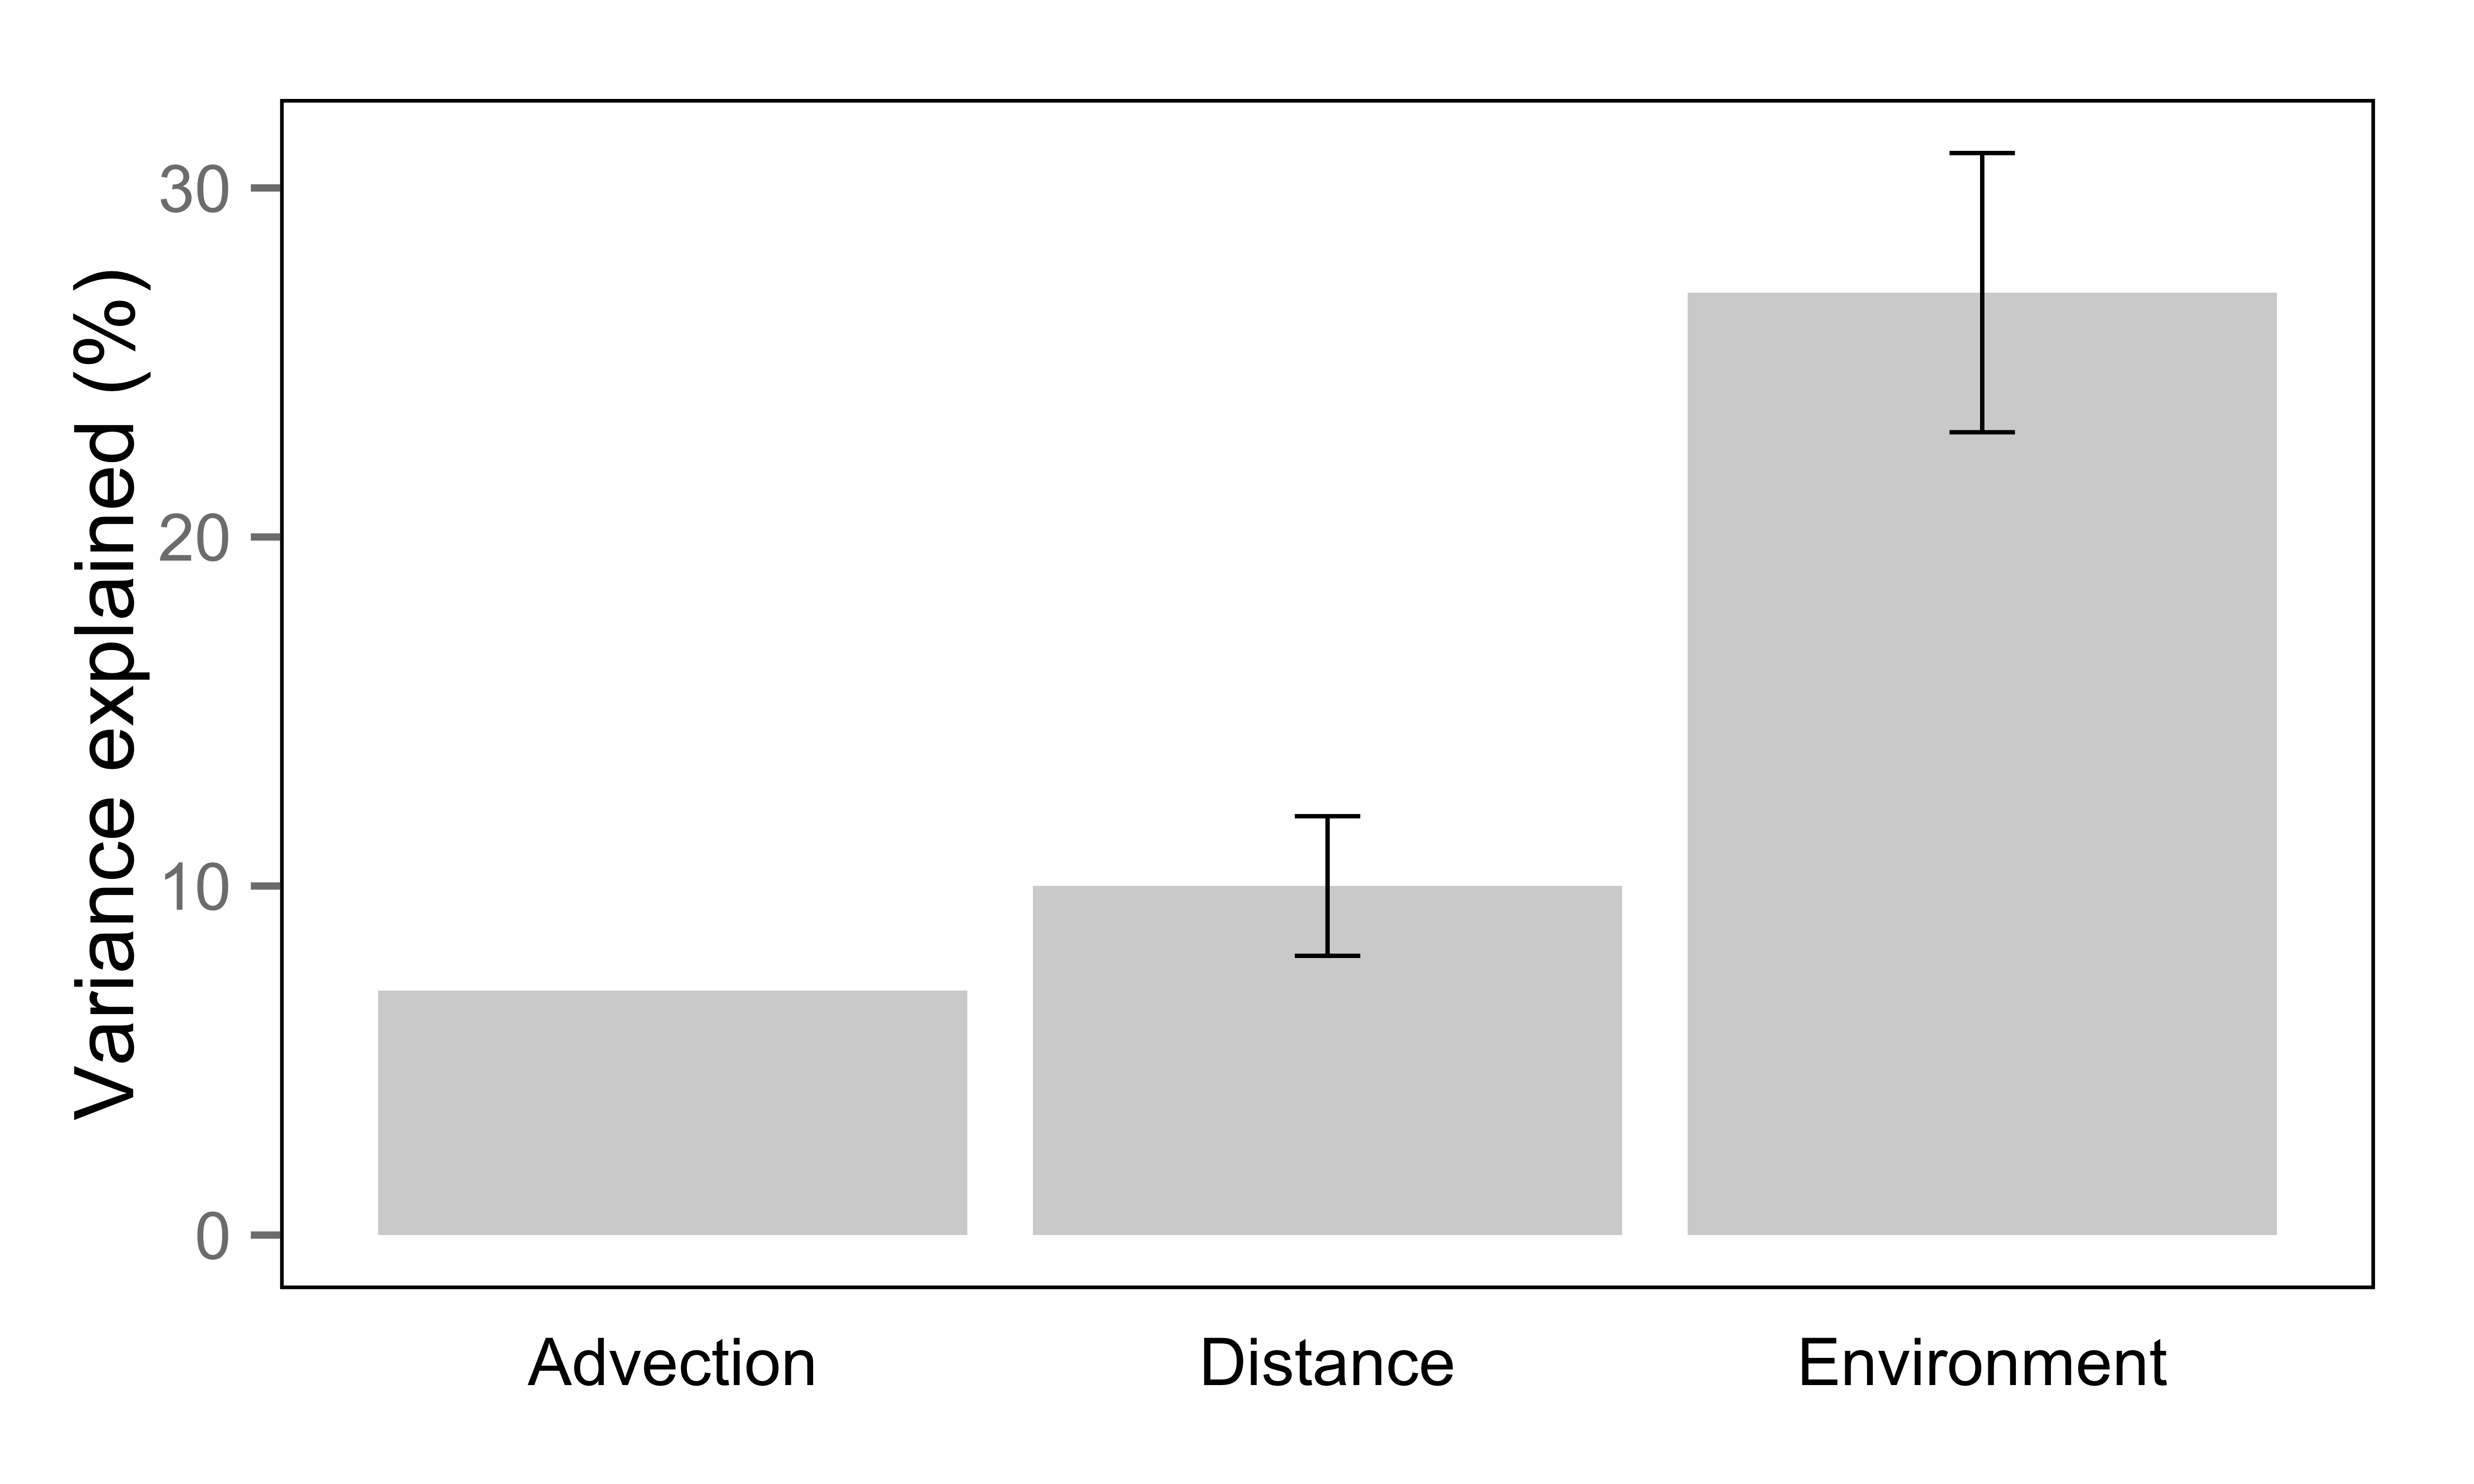
\includegraphics[width=\textwidth]{../generaldiscussion/biogeographybarchart.png}
  \caption[Biogeographic effect sizes]{Variation in microbial community composition explained by environment and distance effects (data from review of 19 studies by \citet{Hanson:2012cb}; error bars represent standard error) and by the advection effect (this study).}
  \label{fig:biogeographybarchart}
\end{figure}


Together, contemporary environmental selection and geographic distance explain \textapprox{} 50\% of variation in microbial community composition \cite{Hanson:2012cb}.
In this study, advection was estimated to explain 7\% of variation \figref{fig:biogeographybarchart}.
This is a conservative estimate, as higher values were found when alternative distance metrics were considered and poorly connected (i.e.\ very deep) samples excluded.
Additionally, it is possible that some samples that were not well connected by advection shared a mutual close advective source \figref{fig:mutualadvectionsource}.

\subsubsection{Future work}

The immediate need for future work on the advection effect is replication, to confirm its existence and measure its magnitude in other oceanic regions.
It is also important that potential alternative explanations for the results, such as the existence of a hidden physicochemical variable (e.g.\ pH, iron concentration) are eliminated by experiments which include measurement of these potential confounds.

Following this, there are several interesting open questions regarding the effect.
In the study described in this thesis, an attempt was made to identify a subset of \acp{OTU} which were more strongly affected by advection than the full set, potentially due to increased resistance to environmental stress and an ability to remain viable over longer distances and times \cite{Bissett:2010wj}.
While such subsets were indeed identified, their biological significance remained ambiguous.
Future work could address this question either by refinement of the statistical methods or with \textit{in vitro} studies of candidate organisms.
While \textit{in situ} cell tracking experiments using the addition of tracer radioisotopes (e.g.\ \ce{^{13}C}) are probably not feasible, it may be possible to use natural radionuclides (e.g.\ \ce{^{234}Th} \cite{Savoye:2005ck} or atmospheric \ce{^{7}Be} \cite{Feng:1999ww}) to the same effect for at least some cell types.

Only bacteria and archaea were included in the community profiles constructed for this study.
This was due to the 0.1--20 \micron{} size range of the sampling method, as well as the complexity of generating reliably commensurate relative abundance estimates using tag pyrosequencing.
However, the addition of unicellular eukaryotes to future studies of the advection effect would be valuable.
Even more interesting would be the effect of advection on marine viruses: bacteriophage have been described as major reservoirs of genetic diversity in the ocean \cite{Suttle:2005bs}, and exchange of genes between phage and host populations may be very common and responsible for the enormous geographic range of identical phage genes \citep[reviewed in][]{Hambly:2005cm}.
However, many virions are labile in the ocean, particularly in surface waters where they are exposed to ultraviolet light, raising the possibility that advection of lysogens may be a vehicle for dispersal of viruses or virus genes across long distances.
Understanding the role of advection in spreading microbial diversity therefore require integrating models of physical transport with gene flow.

\subsection{\softwarename{minspec}}

This thesis also presents a novel software tool, \softwarename{minspec}, which contributes to improving the accuracy of \ac{OTU} assignment and calculation of relative abundances in metagenomic studies.

The number of publicly available full genome sequences for microbial species is growing exponentially: over the course of this project, the number of microbial genomes in the RefSeq database increased from 5,500 (May 2010) to 15,000 (March 2013) (\url{http://www.ncbi.nlm.nih.gov/refseq/statistics/}, accessed 12 April 2013).
As more genomes become available, the number of potential high-quality matches to a given metagenomic read will increase as a natural result of genomic identity between related organisms.
\softwarename{minspec} reduces the need to rely on nucleotide identity as the sole objective standard for assigning metagenomic reads to \acp{OTU}, making use of the contextual information provided by the full set of reads to inform the assignment of each individual read.
While assembly of metagenomic reads can to some extent perform the same function \cite{Temperton:2012fj}, \softwarename{minspec} does not require long or overlapping reads, making it well-suited to the short read lengths of current next-generation sequencing methods and to environments such as the open ocean that have a long tail of low-abundance taxa.

In the long term, single-cell genomic sequencing is the most promising approach for accurate and reliable environmental genomics \cite{Blainey:2013dp} and will likely supplant shotgun sequencing.
Until then, \softwarename{minspec} may be of use in improving the quality of metagenomic results.

\section{The microbial species concept in the ``omics'' age}

In some fortunate disciplines, the intuitive ontologies by which humans ``carve up'' the observed world into conceptual units map well onto the underlying phenomena.
In medicine, for example, the object of study (the human body) is physically divided into easily recognised and discrete units (organs) which have likewise discrete and well-defined functions.
A physician's mental model of the human body has familiar and tangible components, and allows them to understand diseases as systematic divergences from those components' normal form and function.
In physics, on the other hand, such ontologies frequently fail and even mislead.
The vision of electrons as solid spheres orbiting a nucleus like planets around a star holds a strong intuitive appeal, but is contradicted by wave-particle duality, and any physicist who succumbed to this tempting but incorrect view would be more likely to make errors in reasoning.
Physicists, unlike physicians, must either work in new and unfamiliar modes of thinking, or abandon a conceptual grasp of their objects of study altogether and instead investigate them indirectly through mathematical surrogates.

In microbiology, the intuitive unit of study is the cell, and the intuitive category for cells is the species.
Although defining microbial species is not quite as straightforward as for sexually reproducing macroorganisms, the usual standards of 16S and genomic similarity are sufficient for laboratory experiments involving clonal or simple mixed populations in culture.
Environmental microbiologists, in need of a similar unit of categorisation but faced with the diversity and depth of environmental populations, frequently use the \ac{OTU} as a practical method of categorising cells with properties similar enough for the purposes of the scientific question at hand.

The rapidly emerging ``omics'' approaches to environmental microbiology have begun to strain the limits of these categories.
Enormous population sizes, short generation times and the high rate of horizontal gene transfer mean that rather than discrete numbers of distinct \acp{OTU}, microbial assemblages may be better described as ``a continuum of genomic possibilities'' \cite{Goldenfeld:2007im}.
The discovery that many bacterial ``species'' possess ``pan-genomes'', with a conserved ``core'' and dynamic ``variable'' set of genes \cite{Tettelin:2005jg} supports this description.
For example, \citet{Coleman:2010jj} reported large and functionally important differences in the complement of phosphorus acquisition genes within the variable genomes of \genus{Pelagibacter} and \genus{Prochlorococcus} strains in the Atlantic and Pacific oceans.
The traditional species or \ac{OTU} definitions do not map well onto populations of pan-genomic cells, let alone environmental populations with intra- and inter-``species'' fluxes of gene transfer and rapid microevolution.

It may be the case that these new perspectives granted by ``omics'' approaches do not invalidate the species concept, but simply allow systematicists to refine the definition.
\citet{CaroQuintero:2011jv} argue that the cohesive forces on genetic diversity in bacterial populations (periodic selection, suppression of neutral mutations through recombination) are strong enough that cells meaningfully cluster by genomic similarity.
They assert that the species concept remains valid, and is indeed supported by the cohesiveness of these populations when observed with metagenomic analysis; the concept needs only to be adjusted to reduce the emphasis on marker genes (e.g.\ 16S rRNA) and focus more on naturally clustering ``sequence-discrete populations''.
However, when the differences between these ``sequence-discrete'' populations can be described in terms of specific and adaptive gene complements within the variable genome \citep[as in][]{Coleman:2010jj}, the value of forcing these populations into the conceptual box of ``species'', with its attendant historical assumptions and connotations, is questionable.
Should all possible configurations of phosphorous acquisition genes within the variable genome of \genus{Prochlorococcus} --- and if at least two different configurations exist in the tropical Atlantic and Pacific, many more undoubtedly exist elsewhere --- be defined as distinct ``species'' and assigned Latinate binomials?

This is not to argue that the species concept no longer has any merit.
Being able to quickly communicate the relevant features of a cell or population of cells with a simple label will always have great pragmatic value.
The mistake lies in assuming these labels perfectly reflect natural categories, and imposing this assumption on experimental design and analysis.
This is particularly important in the age of ``omics''.
Computers, unlike humans, are not hamstrung by small working memories, and as such have no need to collapse large datasets into simple categories in order to analyse them.
Thus, there are few limits on the accuracy or detail with which microbial populations can be represented \textit{in silico}. 
Given metagenomic or similar environmental data, it is in principle quite possible to model in software a population of dynamic microbial genomes, the gene exchange between these genomes and their relationship to environmental and geographic factors without needing an internal representation of ``species'' or even a cognate such as ``\ac{OTU}''.
To meaningfully investigate (for example) biogeographic patterns in the variable gene complements of pan-genomic microorganisms, imposing the species concept would only be a hindrance.
This is suggested even in some of the results described in this thesis that relied upon the \ac{OTU} as the unit by which cells (or more accurately, genomes) are categorised.
The advection effect (\secreft{ch:advection}) was statistically detectable in 16S-based \ac{OTU} profiles, but attempts to tease out a biologically interesting subset of taxa which were best associated with the effect proved futile.
Given that the effect is likely driven by the dispersal of genomic diversity though small numbers of cells, could it be better modelled as a flux of variable genes through metapopulations of genomically similar cells, of which the changes in \ac{OTU} profiles were only an imperfect reflection?

The recent renewal of activity in microbial biogeography \cite{Ramette:2006jo}, the urgency of environmental change and rapid progress in sequencing technology all create a need to develop better ways to meaningfully describe, categorise and draw conclusions from environmental data \cite{Goldenfeld:2007im}.
As in physics, this may require the reluctant abandonment of intuitive and straightforward conceptual models for a less familiar but more accurate ontology.
Mathematics has benefited in the last four decades from the advent of ``computer-assisted proofs'', which are frequently incomprehensible to human workers but are nevertheless valid and allow progress in otherwise moribund lines of enquiry.
The rapidly increasing volume and complexity of environmental genomic data may mean microbiologists may have to accept a similar trade-off: relinquishing the familiar species concept in exchange for more accurate models of microbial ecosystems.

\section{Conclusions}
This project has demonstrated the role of the \ac{PF} as a major biogeographic barrier in the \ac{SO}.
It has also provided the first direct evidence that the advection of marine microbes influences their community composition.
As well as these results, this thesis contributes methodological advances with the metagenomic tool \softwarename{minspec} and a replicable method for assessing the advection effect in marine systems.
Increased knowledge about fundamental patterns in microbial ecology and biogeography, as well as the specific ecosystem of the \ac{SO}, will be valuable to shaping our response to ecological challenges such as climate change and expanding our understanding of microbial life on Earth.


%bibliography
\singlespacing
\addcontentsline{toc}{chapter}{References}
\bibliographystyle{mybibstyle}
\bibliography{thesis}

\end{document}
